\subsection{Analisi dai dati digitali}
Si è usato il campione preso con il digitizer per fare un confronto tra le misure prese con l'apparato analogico e quelle prese digitalmente.\\
Per prima cosa è stato ricavato un segnale medio per canale, ottenendo così tempo di salita, di discesa e ampiezza media. I due grafici ottenuti sono mostrati in Fig. \ref{gr:mean_signal_0} e Fig. \ref{gr:mean_signal_1}

\begin{tikzpicture}
\pgfdeclareplotmark{cross} {
\pgfpathmoveto{\pgfpoint{-0.3\pgfplotmarksize}{\pgfplotmarksize}}
\pgfpathlineto{\pgfpoint{+0.3\pgfplotmarksize}{\pgfplotmarksize}}
\pgfpathlineto{\pgfpoint{+0.3\pgfplotmarksize}{0.3\pgfplotmarksize}}
\pgfpathlineto{\pgfpoint{+1\pgfplotmarksize}{0.3\pgfplotmarksize}}
\pgfpathlineto{\pgfpoint{+1\pgfplotmarksize}{-0.3\pgfplotmarksize}}
\pgfpathlineto{\pgfpoint{+0.3\pgfplotmarksize}{-0.3\pgfplotmarksize}}
\pgfpathlineto{\pgfpoint{+0.3\pgfplotmarksize}{-1.\pgfplotmarksize}}
\pgfpathlineto{\pgfpoint{-0.3\pgfplotmarksize}{-1.\pgfplotmarksize}}
\pgfpathlineto{\pgfpoint{-0.3\pgfplotmarksize}{-0.3\pgfplotmarksize}}
\pgfpathlineto{\pgfpoint{-1.\pgfplotmarksize}{-0.3\pgfplotmarksize}}
\pgfpathlineto{\pgfpoint{-1.\pgfplotmarksize}{0.3\pgfplotmarksize}}
\pgfpathlineto{\pgfpoint{-0.3\pgfplotmarksize}{0.3\pgfplotmarksize}}
\pgfpathclose
\pgfusepathqstroke
}
\pgfdeclareplotmark{cross*} {
\pgfpathmoveto{\pgfpoint{-0.3\pgfplotmarksize}{\pgfplotmarksize}}
\pgfpathlineto{\pgfpoint{+0.3\pgfplotmarksize}{\pgfplotmarksize}}
\pgfpathlineto{\pgfpoint{+0.3\pgfplotmarksize}{0.3\pgfplotmarksize}}
\pgfpathlineto{\pgfpoint{+1\pgfplotmarksize}{0.3\pgfplotmarksize}}
\pgfpathlineto{\pgfpoint{+1\pgfplotmarksize}{-0.3\pgfplotmarksize}}
\pgfpathlineto{\pgfpoint{+0.3\pgfplotmarksize}{-0.3\pgfplotmarksize}}
\pgfpathlineto{\pgfpoint{+0.3\pgfplotmarksize}{-1.\pgfplotmarksize}}
\pgfpathlineto{\pgfpoint{-0.3\pgfplotmarksize}{-1.\pgfplotmarksize}}
\pgfpathlineto{\pgfpoint{-0.3\pgfplotmarksize}{-0.3\pgfplotmarksize}}
\pgfpathlineto{\pgfpoint{-1.\pgfplotmarksize}{-0.3\pgfplotmarksize}}
\pgfpathlineto{\pgfpoint{-1.\pgfplotmarksize}{0.3\pgfplotmarksize}}
\pgfpathlineto{\pgfpoint{-0.3\pgfplotmarksize}{0.3\pgfplotmarksize}}
\pgfpathclose
\pgfusepathqfillstroke
}
\pgfdeclareplotmark{newstar} {
\pgfpathmoveto{\pgfqpoint{0pt}{\pgfplotmarksize}}
\pgfpathlineto{\pgfqpointpolar{44}{0.5\pgfplotmarksize}}
\pgfpathlineto{\pgfqpointpolar{18}{\pgfplotmarksize}}
\pgfpathlineto{\pgfqpointpolar{-20}{0.5\pgfplotmarksize}}
\pgfpathlineto{\pgfqpointpolar{-54}{\pgfplotmarksize}}
\pgfpathlineto{\pgfqpointpolar{-90}{0.5\pgfplotmarksize}}
\pgfpathlineto{\pgfqpointpolar{234}{\pgfplotmarksize}}
\pgfpathlineto{\pgfqpointpolar{198}{0.5\pgfplotmarksize}}
\pgfpathlineto{\pgfqpointpolar{162}{\pgfplotmarksize}}
\pgfpathlineto{\pgfqpointpolar{134}{0.5\pgfplotmarksize}}
\pgfpathclose
\pgfusepathqstroke
}
\pgfdeclareplotmark{newstar*} {
\pgfpathmoveto{\pgfqpoint{0pt}{\pgfplotmarksize}}
\pgfpathlineto{\pgfqpointpolar{44}{0.5\pgfplotmarksize}}
\pgfpathlineto{\pgfqpointpolar{18}{\pgfplotmarksize}}
\pgfpathlineto{\pgfqpointpolar{-20}{0.5\pgfplotmarksize}}
\pgfpathlineto{\pgfqpointpolar{-54}{\pgfplotmarksize}}
\pgfpathlineto{\pgfqpointpolar{-90}{0.5\pgfplotmarksize}}
\pgfpathlineto{\pgfqpointpolar{234}{\pgfplotmarksize}}
\pgfpathlineto{\pgfqpointpolar{198}{0.5\pgfplotmarksize}}
\pgfpathlineto{\pgfqpointpolar{162}{\pgfplotmarksize}}
\pgfpathlineto{\pgfqpointpolar{134}{0.5\pgfplotmarksize}}
\pgfpathclose
\pgfusepathqfillstroke
}
\definecolor{c}{rgb}{1,1,1};
\draw [color=c, fill=c] (0,0) rectangle (20,11.0085);
\draw [color=c, fill=c] (2,1.10085) rectangle (18,9.90762);
\definecolor{c}{rgb}{0,0,0};
\draw [c,line width=0.9] (2,1.10085) -- (2,9.90762) -- (18,9.90762) -- (18,1.10085) -- (2,1.10085);
\definecolor{c}{rgb}{1,1,1};
\draw [color=c, fill=c] (2,1.10085) rectangle (18,9.90762);
\definecolor{c}{rgb}{0,0,0};
\draw [c,line width=0.9] (2,1.10085) -- (2,9.90762) -- (18,9.90762) -- (18,1.10085) -- (2,1.10085);
\definecolor{c}{rgb}{0,0,0.6};
\draw [c,line width=0.9] (2,9.48742) -- (2.2,9.48742) -- (2.2,9.48742) -- (2.4,9.48742) -- (2.4,9.48742) -- (2.6,9.48742) -- (2.6,9.48742) -- (2.8,9.48742) -- (2.8,9.48742) -- (3,9.48742) -- (3,9.48743) -- (3.2,9.48743) -- (3.2,9.48741) --
 (3.4,9.48741) -- (3.4,9.48743) -- (3.6,9.48743) -- (3.6,9.48742) -- (3.8,9.48742) -- (3.8,9.48743) -- (4,9.48743) -- (4,9.48742) -- (4.2,9.48742) -- (4.2,9.48732) -- (4.4,9.48732) -- (4.4,9.48717) -- (4.6,9.48717) -- (4.6,9.48701) -- (4.8,9.48701)
 -- (4.8,9.4871) -- (5,9.4871) -- (5,9.4872) -- (5.2,9.4872) -- (5.2,9.48722) -- (5.4,9.48722) -- (5.4,9.48686) -- (5.6,9.48686) -- (5.6,9.4866) -- (5.8,9.4866) -- (5.8,9.48634) -- (6,9.48634) -- (6,9.4867) -- (6.2,9.4867) -- (6.2,9.48692) --
 (6.4,9.48692) -- (6.4,9.48716) -- (6.6,9.48716) -- (6.6,9.48721) -- (6.8,9.48721) -- (6.8,9.48726) -- (7,9.48726) -- (7,9.48728) -- (7.2,9.48728) -- (7.2,9.48728) -- (7.4,9.48728) -- (7.4,9.48739) -- (7.6,9.48739) -- (7.6,9.48825) -- (7.8,9.48825)
 -- (7.8,9.42433) -- (8,9.42433) -- (8,6.88473) -- (8.2,6.88473) -- (8.2,1.50025) -- (8.4,1.50025) -- (8.4,3.40203) -- (8.6,3.40203) -- (8.6,5.6249) -- (8.8,5.6249) -- (8.8,7.58763) -- (9,7.58763) -- (9,8.10377) -- (9.2,8.10377) -- (9.2,8.46759) --
 (9.4,8.46759) -- (9.4,8.54405) -- (9.6,8.54405) -- (9.6,8.79529) -- (9.8,8.79529) -- (9.8,9.09477) -- (10,9.09477) -- (10,9.29986) -- (10.2,9.29986) -- (10.2,9.44859) -- (10.4,9.44859) -- (10.4,9.30421) -- (10.6,9.30421) -- (10.6,9.26738) --
 (10.8,9.26738) -- (10.8,9.14727) -- (11,9.14727) -- (11,9.311) -- (11.2,9.311) -- (11.2,9.37002) -- (11.4,9.37002) -- (11.4,9.42704) -- (11.6,9.42704) -- (11.6,9.34394) -- (11.8,9.34394) -- (11.8,9.26105) -- (12,9.26105) -- (12,9.29597) --
 (12.2,9.29597) -- (12.2,9.33515) -- (12.4,9.33515) -- (12.4,9.43142) -- (12.6,9.43142) -- (12.6,9.37374) -- (12.8,9.37374) -- (12.8,9.35255) -- (13,9.35255) -- (13,9.29638) -- (13.2,9.29638) -- (13.2,9.34779) -- (13.4,9.34779) -- (13.4,9.39479) --
 (13.6,9.39479) -- (13.6,9.4125) -- (13.8,9.4125) -- (13.8,9.39562) -- (14,9.39562) -- (14,9.34477) -- (14.2,9.34477) -- (14.2,9.36443) -- (14.4,9.36443) -- (14.4,9.37936) -- (14.6,9.37936) -- (14.6,9.43012) -- (14.8,9.43012) -- (14.8,9.41434) --
 (15,9.41434) -- (15,9.40024) -- (15.2,9.40024) -- (15.2,9.37867) -- (15.4,9.37867) -- (15.4,9.39071) -- (15.6,9.39071) -- (15.6,9.42145) -- (15.8,9.42145) -- (15.8,9.42789) -- (16,9.42789) -- (16,9.42811) -- (16.2,9.42811) -- (16.2,9.40171) --
 (16.4,9.40171) -- (16.4,9.40894) -- (16.6,9.40894) -- (16.6,9.41635) -- (16.8,9.41635) -- (16.8,9.43939) -- (17,9.43939) -- (17,9.43886) -- (17.2,9.43886) -- (17.2,9.42956) -- (17.4,9.42956) -- (17.4,9.42241) -- (17.6,9.42241) -- (17.6,9.42278) --
 (17.8,9.42278) -- (17.8,9.43929) -- (18,9.43929);
\definecolor{c}{rgb}{0,0,0};
\draw [c,line width=0.9] (2,1.10085) -- (18,1.10085);
\draw [anchor= east] (18,0.484373) node[scale=0.854877, color=c, rotate=0]{t [ns]};
\draw [c,line width=0.9] (2,1.36505) -- (2,1.10085);
\draw [c,line width=0.9] (2.5,1.23295) -- (2.5,1.10085);
\draw [c,line width=0.9] (3,1.23295) -- (3,1.10085);
\draw [c,line width=0.9] (3.5,1.23295) -- (3.5,1.10085);
\draw [c,line width=0.9] (4,1.23295) -- (4,1.10085);
\draw [c,line width=0.9] (4.5,1.36505) -- (4.5,1.10085);
\draw [c,line width=0.9] (5,1.23295) -- (5,1.10085);
\draw [c,line width=0.9] (5.5,1.23295) -- (5.5,1.10085);
\draw [c,line width=0.9] (6,1.23295) -- (6,1.10085);
\draw [c,line width=0.9] (6.5,1.23295) -- (6.5,1.10085);
\draw [c,line width=0.9] (7,1.36505) -- (7,1.10085);
\draw [c,line width=0.9] (7.5,1.23295) -- (7.5,1.10085);
\draw [c,line width=0.9] (8,1.23295) -- (8,1.10085);
\draw [c,line width=0.9] (8.5,1.23295) -- (8.5,1.10085);
\draw [c,line width=0.9] (9,1.23295) -- (9,1.10085);
\draw [c,line width=0.9] (9.5,1.36505) -- (9.5,1.10085);
\draw [c,line width=0.9] (10,1.23295) -- (10,1.10085);
\draw [c,line width=0.9] (10.5,1.23295) -- (10.5,1.10085);
\draw [c,line width=0.9] (11,1.23295) -- (11,1.10085);
\draw [c,line width=0.9] (11.5,1.23295) -- (11.5,1.10085);
\draw [c,line width=0.9] (12,1.36505) -- (12,1.10085);
\draw [c,line width=0.9] (12.5,1.23295) -- (12.5,1.10085);
\draw [c,line width=0.9] (13,1.23295) -- (13,1.10085);
\draw [c,line width=0.9] (13.5,1.23295) -- (13.5,1.10085);
\draw [c,line width=0.9] (14,1.23295) -- (14,1.10085);
\draw [c,line width=0.9] (14.5,1.36505) -- (14.5,1.10085);
\draw [c,line width=0.9] (15,1.23295) -- (15,1.10085);
\draw [c,line width=0.9] (15.5,1.23295) -- (15.5,1.10085);
\draw [c,line width=0.9] (16,1.23295) -- (16,1.10085);
\draw [c,line width=0.9] (16.5,1.23295) -- (16.5,1.10085);
\draw [c,line width=0.9] (17,1.36505) -- (17,1.10085);
\draw [c,line width=0.9] (17,1.36505) -- (17,1.10085);
\draw [c,line width=0.9] (17.5,1.23295) -- (17.5,1.10085);
\draw [c,line width=0.9] (18,1.23295) -- (18,1.10085);
\draw [anchor=base] (2,0.737567) node[scale=0.854877, color=c, rotate=0]{0};
\draw [anchor=base] (4.5,0.737567) node[scale=0.854877, color=c, rotate=0]{50};
\draw [anchor=base] (7,0.737567) node[scale=0.854877, color=c, rotate=0]{100};
\draw [anchor=base] (9.5,0.737567) node[scale=0.854877, color=c, rotate=0]{150};
\draw [anchor=base] (12,0.737567) node[scale=0.854877, color=c, rotate=0]{200};
\draw [anchor=base] (14.5,0.737567) node[scale=0.854877, color=c, rotate=0]{250};
\draw [anchor=base] (17,0.737567) node[scale=0.854877, color=c, rotate=0]{300};
\draw [c,line width=0.9] (2,1.10085) -- (2,9.90762);
\draw [anchor= east] (0.88,9.90762) node[scale=0.854877, color=c, rotate=90]{Signal [a.u.]};
\draw [c,line width=0.9] (2.48,1.79993) -- (2,1.79993);
\draw [c,line width=0.9] (2.24,2.01837) -- (2,2.01837);
\draw [c,line width=0.9] (2.24,2.23681) -- (2,2.23681);
\draw [c,line width=0.9] (2.24,2.45525) -- (2,2.45525);
\draw [c,line width=0.9] (2.24,2.67369) -- (2,2.67369);
\draw [c,line width=0.9] (2.48,2.89213) -- (2,2.89213);
\draw [c,line width=0.9] (2.24,3.11056) -- (2,3.11056);
\draw [c,line width=0.9] (2.24,3.329) -- (2,3.329);
\draw [c,line width=0.9] (2.24,3.54744) -- (2,3.54744);
\draw [c,line width=0.9] (2.24,3.76588) -- (2,3.76588);
\draw [c,line width=0.9] (2.48,3.98432) -- (2,3.98432);
\draw [c,line width=0.9] (2.24,4.20276) -- (2,4.20276);
\draw [c,line width=0.9] (2.24,4.42119) -- (2,4.42119);
\draw [c,line width=0.9] (2.24,4.63963) -- (2,4.63963);
\draw [c,line width=0.9] (2.24,4.85807) -- (2,4.85807);
\draw [c,line width=0.9] (2.48,5.07651) -- (2,5.07651);
\draw [c,line width=0.9] (2.24,5.29495) -- (2,5.29495);
\draw [c,line width=0.9] (2.24,5.51339) -- (2,5.51339);
\draw [c,line width=0.9] (2.24,5.73182) -- (2,5.73182);
\draw [c,line width=0.9] (2.24,5.95026) -- (2,5.95026);
\draw [c,line width=0.9] (2.48,6.1687) -- (2,6.1687);
\draw [c,line width=0.9] (2.24,6.38714) -- (2,6.38714);
\draw [c,line width=0.9] (2.24,6.60558) -- (2,6.60558);
\draw [c,line width=0.9] (2.24,6.82402) -- (2,6.82402);
\draw [c,line width=0.9] (2.24,7.04245) -- (2,7.04245);
\draw [c,line width=0.9] (2.48,7.26089) -- (2,7.26089);
\draw [c,line width=0.9] (2.24,7.47933) -- (2,7.47933);
\draw [c,line width=0.9] (2.24,7.69777) -- (2,7.69777);
\draw [c,line width=0.9] (2.24,7.91621) -- (2,7.91621);
\draw [c,line width=0.9] (2.24,8.13464) -- (2,8.13464);
\draw [c,line width=0.9] (2.48,8.35308) -- (2,8.35308);
\draw [c,line width=0.9] (2.24,8.57152) -- (2,8.57152);
\draw [c,line width=0.9] (2.24,8.78996) -- (2,8.78996);
\draw [c,line width=0.9] (2.24,9.0084) -- (2,9.0084);
\draw [c,line width=0.9] (2.24,9.22684) -- (2,9.22684);
\draw [c,line width=0.9] (2.48,9.44528) -- (2,9.44528);
\draw [c,line width=0.9] (2.48,1.79993) -- (2,1.79993);
\draw [c,line width=0.9] (2.24,1.5815) -- (2,1.5815);
\draw [c,line width=0.9] (2.24,1.36306) -- (2,1.36306);
\draw [c,line width=0.9] (2.24,1.14462) -- (2,1.14462);
\draw [c,line width=0.9] (2.48,9.44528) -- (2,9.44528);
\draw [c,line width=0.9] (2.24,9.66371) -- (2,9.66371);
\draw [c,line width=0.9] (2.24,9.88215) -- (2,9.88215);
\draw [anchor= east] (1.9,1.79993) node[scale=0.854877, color=c, rotate=0]{2900};
\draw [anchor= east] (1.9,2.89213) node[scale=0.854877, color=c, rotate=0]{3000};
\draw [anchor= east] (1.9,3.98432) node[scale=0.854877, color=c, rotate=0]{3100};
\draw [anchor= east] (1.9,5.07651) node[scale=0.854877, color=c, rotate=0]{3200};
\draw [anchor= east] (1.9,6.1687) node[scale=0.854877, color=c, rotate=0]{3300};
\draw [anchor= east] (1.9,7.26089) node[scale=0.854877, color=c, rotate=0]{3400};
\draw [anchor= east] (1.9,8.35308) node[scale=0.854877, color=c, rotate=0]{3500};
\draw [anchor= east] (1.9,9.44528) node[scale=0.854877, color=c, rotate=0]{3600};
\end{tikzpicture}

\begin{tikzpicture}
\pgfdeclareplotmark{cross} {
\pgfpathmoveto{\pgfpoint{-0.3\pgfplotmarksize}{\pgfplotmarksize}}
\pgfpathlineto{\pgfpoint{+0.3\pgfplotmarksize}{\pgfplotmarksize}}
\pgfpathlineto{\pgfpoint{+0.3\pgfplotmarksize}{0.3\pgfplotmarksize}}
\pgfpathlineto{\pgfpoint{+1\pgfplotmarksize}{0.3\pgfplotmarksize}}
\pgfpathlineto{\pgfpoint{+1\pgfplotmarksize}{-0.3\pgfplotmarksize}}
\pgfpathlineto{\pgfpoint{+0.3\pgfplotmarksize}{-0.3\pgfplotmarksize}}
\pgfpathlineto{\pgfpoint{+0.3\pgfplotmarksize}{-1.\pgfplotmarksize}}
\pgfpathlineto{\pgfpoint{-0.3\pgfplotmarksize}{-1.\pgfplotmarksize}}
\pgfpathlineto{\pgfpoint{-0.3\pgfplotmarksize}{-0.3\pgfplotmarksize}}
\pgfpathlineto{\pgfpoint{-1.\pgfplotmarksize}{-0.3\pgfplotmarksize}}
\pgfpathlineto{\pgfpoint{-1.\pgfplotmarksize}{0.3\pgfplotmarksize}}
\pgfpathlineto{\pgfpoint{-0.3\pgfplotmarksize}{0.3\pgfplotmarksize}}
\pgfpathclose
\pgfusepathqstroke
}
\pgfdeclareplotmark{cross*} {
\pgfpathmoveto{\pgfpoint{-0.3\pgfplotmarksize}{\pgfplotmarksize}}
\pgfpathlineto{\pgfpoint{+0.3\pgfplotmarksize}{\pgfplotmarksize}}
\pgfpathlineto{\pgfpoint{+0.3\pgfplotmarksize}{0.3\pgfplotmarksize}}
\pgfpathlineto{\pgfpoint{+1\pgfplotmarksize}{0.3\pgfplotmarksize}}
\pgfpathlineto{\pgfpoint{+1\pgfplotmarksize}{-0.3\pgfplotmarksize}}
\pgfpathlineto{\pgfpoint{+0.3\pgfplotmarksize}{-0.3\pgfplotmarksize}}
\pgfpathlineto{\pgfpoint{+0.3\pgfplotmarksize}{-1.\pgfplotmarksize}}
\pgfpathlineto{\pgfpoint{-0.3\pgfplotmarksize}{-1.\pgfplotmarksize}}
\pgfpathlineto{\pgfpoint{-0.3\pgfplotmarksize}{-0.3\pgfplotmarksize}}
\pgfpathlineto{\pgfpoint{-1.\pgfplotmarksize}{-0.3\pgfplotmarksize}}
\pgfpathlineto{\pgfpoint{-1.\pgfplotmarksize}{0.3\pgfplotmarksize}}
\pgfpathlineto{\pgfpoint{-0.3\pgfplotmarksize}{0.3\pgfplotmarksize}}
\pgfpathclose
\pgfusepathqfillstroke
}
\pgfdeclareplotmark{newstar} {
\pgfpathmoveto{\pgfqpoint{0pt}{\pgfplotmarksize}}
\pgfpathlineto{\pgfqpointpolar{44}{0.5\pgfplotmarksize}}
\pgfpathlineto{\pgfqpointpolar{18}{\pgfplotmarksize}}
\pgfpathlineto{\pgfqpointpolar{-20}{0.5\pgfplotmarksize}}
\pgfpathlineto{\pgfqpointpolar{-54}{\pgfplotmarksize}}
\pgfpathlineto{\pgfqpointpolar{-90}{0.5\pgfplotmarksize}}
\pgfpathlineto{\pgfqpointpolar{234}{\pgfplotmarksize}}
\pgfpathlineto{\pgfqpointpolar{198}{0.5\pgfplotmarksize}}
\pgfpathlineto{\pgfqpointpolar{162}{\pgfplotmarksize}}
\pgfpathlineto{\pgfqpointpolar{134}{0.5\pgfplotmarksize}}
\pgfpathclose
\pgfusepathqstroke
}
\pgfdeclareplotmark{newstar*} {
\pgfpathmoveto{\pgfqpoint{0pt}{\pgfplotmarksize}}
\pgfpathlineto{\pgfqpointpolar{44}{0.5\pgfplotmarksize}}
\pgfpathlineto{\pgfqpointpolar{18}{\pgfplotmarksize}}
\pgfpathlineto{\pgfqpointpolar{-20}{0.5\pgfplotmarksize}}
\pgfpathlineto{\pgfqpointpolar{-54}{\pgfplotmarksize}}
\pgfpathlineto{\pgfqpointpolar{-90}{0.5\pgfplotmarksize}}
\pgfpathlineto{\pgfqpointpolar{234}{\pgfplotmarksize}}
\pgfpathlineto{\pgfqpointpolar{198}{0.5\pgfplotmarksize}}
\pgfpathlineto{\pgfqpointpolar{162}{\pgfplotmarksize}}
\pgfpathlineto{\pgfqpointpolar{134}{0.5\pgfplotmarksize}}
\pgfpathclose
\pgfusepathqfillstroke
}
\definecolor{c}{rgb}{1,1,1};
\draw [color=c, fill=c] (0,0) rectangle (20,11.0085);
\draw [color=c, fill=c] (2,1.10085) rectangle (18,9.90762);
\definecolor{c}{rgb}{0,0,0};
\draw [c,line width=0.9] (2,1.10085) -- (2,9.90762) -- (18,9.90762) -- (18,1.10085) -- (2,1.10085);
\definecolor{c}{rgb}{1,1,1};
\draw [color=c, fill=c] (2,1.10085) rectangle (18,9.90762);
\definecolor{c}{rgb}{0,0,0};
\draw [c,line width=0.9] (2,1.10085) -- (2,9.90762) -- (18,9.90762) -- (18,1.10085) -- (2,1.10085);
\definecolor{c}{rgb}{0,0,0.6};
\draw [c,line width=0.9] (2,9.48718) -- (2.2,9.48718) -- (2.2,9.48719) -- (2.4,9.48719) -- (2.4,9.48718) -- (2.6,9.48718) -- (2.6,9.48719) -- (2.8,9.48719) -- (2.8,9.4872) -- (3,9.4872) -- (3,9.48718) -- (3.2,9.48718) -- (3.2,9.48719) --
 (3.4,9.48719) -- (3.4,9.48719) -- (3.6,9.48719) -- (3.6,9.48719) -- (3.8,9.48719) -- (3.8,9.48719) -- (4,9.48719) -- (4,9.48719) -- (4.2,9.48719) -- (4.2,9.48717) -- (4.4,9.48717) -- (4.4,9.48696) -- (4.6,9.48696) -- (4.6,9.4868) -- (4.8,9.4868) --
 (4.8,9.48686) -- (5,9.48686) -- (5,9.48699) -- (5.2,9.48699) -- (5.2,9.48708) -- (5.4,9.48708) -- (5.4,9.48691) -- (5.6,9.48691) -- (5.6,9.48656) -- (5.8,9.48656) -- (5.8,9.48627) -- (6,9.48627) -- (6,9.48657) -- (6.2,9.48657) -- (6.2,9.4868) --
 (6.4,9.4868) -- (6.4,9.487) -- (6.6,9.487) -- (6.6,9.48703) -- (6.8,9.48703) -- (6.8,9.48703) -- (7,9.48703) -- (7,9.48704) -- (7.2,9.48704) -- (7.2,9.48705) -- (7.4,9.48705) -- (7.4,9.48715) -- (7.6,9.48715) -- (7.6,9.48825) -- (7.8,9.48825) --
 (7.8,9.41639) -- (8,9.41639) -- (8,6.64755) -- (8.2,6.64755) -- (8.2,1.50025) -- (8.4,1.50025) -- (8.4,3.6606) -- (8.6,3.6606) -- (8.6,5.81757) -- (8.8,5.81757) -- (8.8,7.7531) -- (9,7.7531) -- (9,8.51018) -- (9.2,8.51018) -- (9.2,8.91869) --
 (9.4,8.91869) -- (9.4,8.91475) -- (9.6,8.91475) -- (9.6,8.84305) -- (9.8,8.84305) -- (9.8,9.15593) -- (10,9.15593) -- (10,9.34825) -- (10.2,9.34825) -- (10.2,9.46495) -- (10.4,9.46495) -- (10.4,9.29036) -- (10.6,9.29036) -- (10.6,9.17963) --
 (10.8,9.17963) -- (10.8,9.19589) -- (11,9.19589) -- (11,9.31088) -- (11.2,9.31088) -- (11.2,9.43531) -- (11.4,9.43531) -- (11.4,9.34894) -- (11.6,9.34894) -- (11.6,9.28068) -- (11.8,9.28068) -- (11.8,9.22939) -- (12,9.22939) -- (12,9.3142) --
 (12.2,9.3142) -- (12.2,9.40517) -- (12.4,9.40517) -- (12.4,9.38847) -- (12.6,9.38847) -- (12.6,9.34441) -- (12.8,9.34441) -- (12.8,9.27973) -- (13,9.27973) -- (13,9.32617) -- (13.2,9.32617) -- (13.2,9.38578) -- (13.4,9.38578) -- (13.4,9.40897) --
 (13.6,9.40897) -- (13.6,9.38084) -- (13.8,9.38084) -- (13.8,9.32885) -- (14,9.32885) -- (14,9.34356) -- (14.2,9.34356) -- (14.2,9.37859) -- (14.4,9.37859) -- (14.4,9.41625) -- (14.6,9.41625) -- (14.6,9.40285) -- (14.8,9.40285) -- (14.8,9.37059) --
 (15,9.37059) -- (15,9.36481) -- (15.2,9.36481) -- (15.2,9.3841) -- (15.4,9.3841) -- (15.4,9.41908) -- (15.6,9.41908) -- (15.6,9.41745) -- (15.8,9.41745) -- (15.8,9.40115) -- (16,9.40115) -- (16,9.38652) -- (16.2,9.38652) -- (16.2,9.39608) --
 (16.4,9.39608) -- (16.4,9.42071) -- (16.6,9.42071) -- (16.6,9.42814) -- (16.8,9.42814) -- (16.8,9.42178) -- (17,9.42178) -- (17,9.40772) -- (17.2,9.40772) -- (17.2,9.41047) -- (17.4,9.41047) -- (17.4,9.42549) -- (17.6,9.42549) -- (17.6,9.43648) --
 (17.8,9.43648) -- (17.8,9.4356) -- (18,9.4356);
\definecolor{c}{rgb}{0,0,0};
\draw [c,line width=0.9] (2,1.10085) -- (18,1.10085);
\draw [anchor= east] (18,0.484373) node[scale=0.854877, color=c, rotate=0]{t [ns]};
\draw [c,line width=0.9] (2,1.36505) -- (2,1.10085);
\draw [c,line width=0.9] (2.5,1.23295) -- (2.5,1.10085);
\draw [c,line width=0.9] (3,1.23295) -- (3,1.10085);
\draw [c,line width=0.9] (3.5,1.23295) -- (3.5,1.10085);
\draw [c,line width=0.9] (4,1.23295) -- (4,1.10085);
\draw [c,line width=0.9] (4.5,1.36505) -- (4.5,1.10085);
\draw [c,line width=0.9] (5,1.23295) -- (5,1.10085);
\draw [c,line width=0.9] (5.5,1.23295) -- (5.5,1.10085);
\draw [c,line width=0.9] (6,1.23295) -- (6,1.10085);
\draw [c,line width=0.9] (6.5,1.23295) -- (6.5,1.10085);
\draw [c,line width=0.9] (7,1.36505) -- (7,1.10085);
\draw [c,line width=0.9] (7.5,1.23295) -- (7.5,1.10085);
\draw [c,line width=0.9] (8,1.23295) -- (8,1.10085);
\draw [c,line width=0.9] (8.5,1.23295) -- (8.5,1.10085);
\draw [c,line width=0.9] (9,1.23295) -- (9,1.10085);
\draw [c,line width=0.9] (9.5,1.36505) -- (9.5,1.10085);
\draw [c,line width=0.9] (10,1.23295) -- (10,1.10085);
\draw [c,line width=0.9] (10.5,1.23295) -- (10.5,1.10085);
\draw [c,line width=0.9] (11,1.23295) -- (11,1.10085);
\draw [c,line width=0.9] (11.5,1.23295) -- (11.5,1.10085);
\draw [c,line width=0.9] (12,1.36505) -- (12,1.10085);
\draw [c,line width=0.9] (12.5,1.23295) -- (12.5,1.10085);
\draw [c,line width=0.9] (13,1.23295) -- (13,1.10085);
\draw [c,line width=0.9] (13.5,1.23295) -- (13.5,1.10085);
\draw [c,line width=0.9] (14,1.23295) -- (14,1.10085);
\draw [c,line width=0.9] (14.5,1.36505) -- (14.5,1.10085);
\draw [c,line width=0.9] (15,1.23295) -- (15,1.10085);
\draw [c,line width=0.9] (15.5,1.23295) -- (15.5,1.10085);
\draw [c,line width=0.9] (16,1.23295) -- (16,1.10085);
\draw [c,line width=0.9] (16.5,1.23295) -- (16.5,1.10085);
\draw [c,line width=0.9] (17,1.36505) -- (17,1.10085);
\draw [c,line width=0.9] (17,1.36505) -- (17,1.10085);
\draw [c,line width=0.9] (17.5,1.23295) -- (17.5,1.10085);
\draw [c,line width=0.9] (18,1.23295) -- (18,1.10085);
\draw [anchor=base] (2,0.737567) node[scale=0.854877, color=c, rotate=0]{0};
\draw [anchor=base] (4.5,0.737567) node[scale=0.854877, color=c, rotate=0]{50};
\draw [anchor=base] (7,0.737567) node[scale=0.854877, color=c, rotate=0]{100};
\draw [anchor=base] (9.5,0.737567) node[scale=0.854877, color=c, rotate=0]{150};
\draw [anchor=base] (12,0.737567) node[scale=0.854877, color=c, rotate=0]{200};
\draw [anchor=base] (14.5,0.737567) node[scale=0.854877, color=c, rotate=0]{250};
\draw [anchor=base] (17,0.737567) node[scale=0.854877, color=c, rotate=0]{300};
\draw [c,line width=0.9] (2,1.10085) -- (2,9.90762);
\draw [anchor= east] (0.88,9.90762) node[scale=0.854877, color=c, rotate=90]{Signal [a.u.]};
\draw [c,line width=0.9] (2.48,1.1948) -- (2,1.1948);
\draw [c,line width=0.9] (2.24,1.44684) -- (2,1.44684);
\draw [c,line width=0.9] (2.24,1.69889) -- (2,1.69889);
\draw [c,line width=0.9] (2.24,1.95093) -- (2,1.95093);
\draw [c,line width=0.9] (2.24,2.20298) -- (2,2.20298);
\draw [c,line width=0.9] (2.48,2.45502) -- (2,2.45502);
\draw [c,line width=0.9] (2.24,2.70707) -- (2,2.70707);
\draw [c,line width=0.9] (2.24,2.95912) -- (2,2.95912);
\draw [c,line width=0.9] (2.24,3.21116) -- (2,3.21116);
\draw [c,line width=0.9] (2.24,3.46321) -- (2,3.46321);
\draw [c,line width=0.9] (2.48,3.71525) -- (2,3.71525);
\draw [c,line width=0.9] (2.24,3.9673) -- (2,3.9673);
\draw [c,line width=0.9] (2.24,4.21934) -- (2,4.21934);
\draw [c,line width=0.9] (2.24,4.47139) -- (2,4.47139);
\draw [c,line width=0.9] (2.24,4.72344) -- (2,4.72344);
\draw [c,line width=0.9] (2.48,4.97548) -- (2,4.97548);
\draw [c,line width=0.9] (2.24,5.22753) -- (2,5.22753);
\draw [c,line width=0.9] (2.24,5.47957) -- (2,5.47957);
\draw [c,line width=0.9] (2.24,5.73162) -- (2,5.73162);
\draw [c,line width=0.9] (2.24,5.98366) -- (2,5.98366);
\draw [c,line width=0.9] (2.48,6.23571) -- (2,6.23571);
\draw [c,line width=0.9] (2.24,6.48775) -- (2,6.48775);
\draw [c,line width=0.9] (2.24,6.7398) -- (2,6.7398);
\draw [c,line width=0.9] (2.24,6.99185) -- (2,6.99185);
\draw [c,line width=0.9] (2.24,7.24389) -- (2,7.24389);
\draw [c,line width=0.9] (2.48,7.49594) -- (2,7.49594);
\draw [c,line width=0.9] (2.24,7.74798) -- (2,7.74798);
\draw [c,line width=0.9] (2.24,8.00003) -- (2,8.00003);
\draw [c,line width=0.9] (2.24,8.25207) -- (2,8.25207);
\draw [c,line width=0.9] (2.24,8.50412) -- (2,8.50412);
\draw [c,line width=0.9] (2.48,8.75617) -- (2,8.75617);
\draw [c,line width=0.9] (2.48,1.1948) -- (2,1.1948);
\draw [c,line width=0.9] (2.48,8.75617) -- (2,8.75617);
\draw [c,line width=0.9] (2.24,9.00821) -- (2,9.00821);
\draw [c,line width=0.9] (2.24,9.26026) -- (2,9.26026);
\draw [c,line width=0.9] (2.24,9.5123) -- (2,9.5123);
\draw [c,line width=0.9] (2.24,9.76435) -- (2,9.76435);
\draw [anchor= east] (1.9,1.1948) node[scale=0.854877, color=c, rotate=0]{3100};
\draw [anchor= east] (1.9,2.45502) node[scale=0.854877, color=c, rotate=0]{3200};
\draw [anchor= east] (1.9,3.71525) node[scale=0.854877, color=c, rotate=0]{3300};
\draw [anchor= east] (1.9,4.97548) node[scale=0.854877, color=c, rotate=0]{3400};
\draw [anchor= east] (1.9,6.23571) node[scale=0.854877, color=c, rotate=0]{3500};
\draw [anchor= east] (1.9,7.49594) node[scale=0.854877, color=c, rotate=0]{3600};
\draw [anchor= east] (1.9,8.75617) node[scale=0.854877, color=c, rotate=0]{3700};
\definecolor{c}{rgb}{1,1,1};
\draw [color=c, fill=c] (15.6,8.53156) rectangle (19.6,10.2929);
\definecolor{c}{rgb}{0,0,0};
\draw [c,line width=0.9] (15.6,8.53156) -- (19.6,8.53156);
\draw [c,line width=0.9] (19.6,8.53156) -- (19.6,10.2929);
\draw [c,line width=0.9] (19.6,10.2929) -- (15.6,10.2929);
\draw [c,line width=0.9] (15.6,10.2929) -- (15.6,8.53156);
\draw (17.6,10.0727) node[scale=0.889072, color=c, rotate=0]{MeanSignalCh1};
\draw [c,line width=0.9] (15.6,9.85258) -- (19.6,9.85258);
\draw [anchor= west] (15.8,9.63241) node[scale=0.889072, color=c, rotate=0]{Entries };
\draw [anchor= east] (19.4,9.63241) node[scale=0.889072, color=c, rotate=0]{ 0};
\draw [anchor= west] (15.8,9.19207) node[scale=0.889072, color=c, rotate=0]{Mean  };
\draw [anchor= east] (19.4,9.19207) node[scale=0.889072, color=c, rotate=0]{      0};
\draw [anchor= west] (15.8,8.75173) node[scale=0.889072, color=c, rotate=0]{Std Dev   };
\draw [anchor= east] (19.4,8.75173) node[scale=0.889072, color=c, rotate=0]{      0};
\end{tikzpicture}


Tabella bella

Filtrando dal campione solo gli eventi in coincidenza (presa contando gli eventi il cui time tag differisse meno di 100 ns), si è poi fatta un analisi della risoluzione temporale dell'apparato digitale. Per le misure di tempo si è usato un algoritmo simile al CFTD analogico, facendo variare il ritardo tra i 4 e i 12 ns e l'attenuazione tra lo 0.2 e lo 0.8. Per la ricerca del punto di zero cressing si è fatta un interpolazione con una cubica tra i punti di massimo e minimo del segnale di ``CF monitor'', dato che l'interpolazione suggerita con una retta aveva diversi problemi dovuti alla bassa frequenza di campionamento (vedi Fig. \ref{gr:fail_retta_interp}) che davano una distribuzione temporale distorta.
Le distribuzioni ottenute al variare dei parametri sono state sovrapposte in Fig. \ref{hist:confronto_ris_temp_digi}, mostrando che la risoluzione migliore si ha quando il ritardo è di 4 ns e l'attenuazione è a 0.3. Dato però che questa distribuzione risulta essere leggermente deformata, si è preferito usare l'attenuazione a 0.4, la seconda migliore.

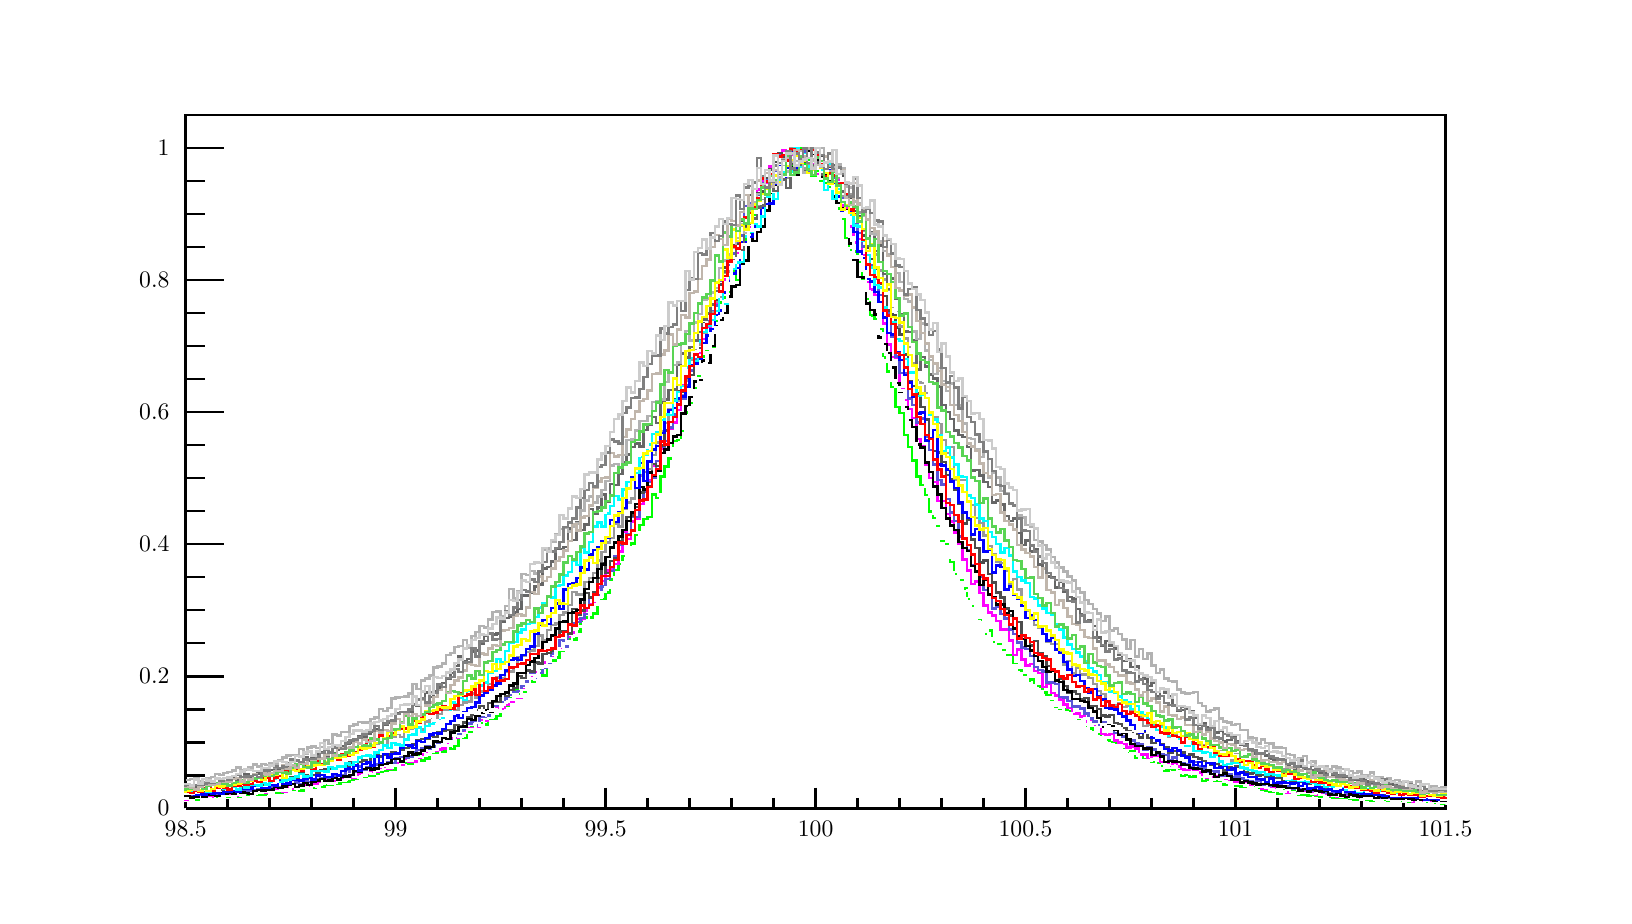
\begin{tikzpicture}
\pgfdeclareplotmark{cross} {
\pgfpathmoveto{\pgfpoint{-0.3\pgfplotmarksize}{\pgfplotmarksize}}
\pgfpathlineto{\pgfpoint{+0.3\pgfplotmarksize}{\pgfplotmarksize}}
\pgfpathlineto{\pgfpoint{+0.3\pgfplotmarksize}{0.3\pgfplotmarksize}}
\pgfpathlineto{\pgfpoint{+1\pgfplotmarksize}{0.3\pgfplotmarksize}}
\pgfpathlineto{\pgfpoint{+1\pgfplotmarksize}{-0.3\pgfplotmarksize}}
\pgfpathlineto{\pgfpoint{+0.3\pgfplotmarksize}{-0.3\pgfplotmarksize}}
\pgfpathlineto{\pgfpoint{+0.3\pgfplotmarksize}{-1.\pgfplotmarksize}}
\pgfpathlineto{\pgfpoint{-0.3\pgfplotmarksize}{-1.\pgfplotmarksize}}
\pgfpathlineto{\pgfpoint{-0.3\pgfplotmarksize}{-0.3\pgfplotmarksize}}
\pgfpathlineto{\pgfpoint{-1.\pgfplotmarksize}{-0.3\pgfplotmarksize}}
\pgfpathlineto{\pgfpoint{-1.\pgfplotmarksize}{0.3\pgfplotmarksize}}
\pgfpathlineto{\pgfpoint{-0.3\pgfplotmarksize}{0.3\pgfplotmarksize}}
\pgfpathclose
\pgfusepathqstroke
}
\pgfdeclareplotmark{cross*} {
\pgfpathmoveto{\pgfpoint{-0.3\pgfplotmarksize}{\pgfplotmarksize}}
\pgfpathlineto{\pgfpoint{+0.3\pgfplotmarksize}{\pgfplotmarksize}}
\pgfpathlineto{\pgfpoint{+0.3\pgfplotmarksize}{0.3\pgfplotmarksize}}
\pgfpathlineto{\pgfpoint{+1\pgfplotmarksize}{0.3\pgfplotmarksize}}
\pgfpathlineto{\pgfpoint{+1\pgfplotmarksize}{-0.3\pgfplotmarksize}}
\pgfpathlineto{\pgfpoint{+0.3\pgfplotmarksize}{-0.3\pgfplotmarksize}}
\pgfpathlineto{\pgfpoint{+0.3\pgfplotmarksize}{-1.\pgfplotmarksize}}
\pgfpathlineto{\pgfpoint{-0.3\pgfplotmarksize}{-1.\pgfplotmarksize}}
\pgfpathlineto{\pgfpoint{-0.3\pgfplotmarksize}{-0.3\pgfplotmarksize}}
\pgfpathlineto{\pgfpoint{-1.\pgfplotmarksize}{-0.3\pgfplotmarksize}}
\pgfpathlineto{\pgfpoint{-1.\pgfplotmarksize}{0.3\pgfplotmarksize}}
\pgfpathlineto{\pgfpoint{-0.3\pgfplotmarksize}{0.3\pgfplotmarksize}}
\pgfpathclose
\pgfusepathqfillstroke
}
\pgfdeclareplotmark{newstar} {
\pgfpathmoveto{\pgfqpoint{0pt}{\pgfplotmarksize}}
\pgfpathlineto{\pgfqpointpolar{44}{0.5\pgfplotmarksize}}
\pgfpathlineto{\pgfqpointpolar{18}{\pgfplotmarksize}}
\pgfpathlineto{\pgfqpointpolar{-20}{0.5\pgfplotmarksize}}
\pgfpathlineto{\pgfqpointpolar{-54}{\pgfplotmarksize}}
\pgfpathlineto{\pgfqpointpolar{-90}{0.5\pgfplotmarksize}}
\pgfpathlineto{\pgfqpointpolar{234}{\pgfplotmarksize}}
\pgfpathlineto{\pgfqpointpolar{198}{0.5\pgfplotmarksize}}
\pgfpathlineto{\pgfqpointpolar{162}{\pgfplotmarksize}}
\pgfpathlineto{\pgfqpointpolar{134}{0.5\pgfplotmarksize}}
\pgfpathclose
\pgfusepathqstroke
}
\pgfdeclareplotmark{newstar*} {
\pgfpathmoveto{\pgfqpoint{0pt}{\pgfplotmarksize}}
\pgfpathlineto{\pgfqpointpolar{44}{0.5\pgfplotmarksize}}
\pgfpathlineto{\pgfqpointpolar{18}{\pgfplotmarksize}}
\pgfpathlineto{\pgfqpointpolar{-20}{0.5\pgfplotmarksize}}
\pgfpathlineto{\pgfqpointpolar{-54}{\pgfplotmarksize}}
\pgfpathlineto{\pgfqpointpolar{-90}{0.5\pgfplotmarksize}}
\pgfpathlineto{\pgfqpointpolar{234}{\pgfplotmarksize}}
\pgfpathlineto{\pgfqpointpolar{198}{0.5\pgfplotmarksize}}
\pgfpathlineto{\pgfqpointpolar{162}{\pgfplotmarksize}}
\pgfpathlineto{\pgfqpointpolar{134}{0.5\pgfplotmarksize}}
\pgfpathclose
\pgfusepathqfillstroke
}
\definecolor{c}{rgb}{1,1,1};
\draw [color=c, fill=c] (0,0) rectangle (20,11.0085);
\draw [color=c, fill=c] (2,1.10085) rectangle (18,9.90762);
\definecolor{c}{rgb}{0,0,0};
\draw [c,line width=0.9] (2,1.10085) -- (2,9.90762) -- (18,9.90762) -- (18,1.10085) -- (2,1.10085);
\definecolor{c}{rgb}{1,1,1};
\draw [color=c, fill=c] (2,1.10085) rectangle (18,9.90762);
\definecolor{c}{rgb}{0,0,0};
\draw [c,line width=0.9] (2,1.10085) -- (2,9.90762) -- (18,9.90762) -- (18,1.10085) -- (2,1.10085);
\definecolor{c}{rgb}{1,1,1};
\draw [c,line width=0.9] (2,1.21589) -- (2.05333,1.21589) -- (2.05333,1.20866) -- (2.10667,1.20866) -- (2.10667,1.21589) -- (2.16,1.21589) -- (2.16,1.23543) -- (2.21333,1.23543) -- (2.21333,1.23036) -- (2.26667,1.23036) -- (2.26667,1.23181) --
 (2.32,1.23181) -- (2.32,1.24773) -- (2.37333,1.24773) -- (2.37333,1.2347) -- (2.42667,1.2347) -- (2.42667,1.24194) -- (2.48,1.24194) -- (2.48,1.26871) -- (2.53333,1.26871) -- (2.53333,1.26726) -- (2.58667,1.26726) -- (2.58667,1.25062) --
 (2.64,1.25062) -- (2.64,1.2622) -- (2.69333,1.2622) -- (2.69333,1.27667) -- (2.74667,1.27667) -- (2.74667,1.27667) -- (2.8,1.27667) -- (2.8,1.27812) -- (2.85333,1.27812) -- (2.85333,1.30127) -- (2.90667,1.30127) -- (2.90667,1.32081) --
 (2.96,1.32081) -- (2.96,1.31502) -- (3.01333,1.31502) -- (3.01333,1.29042) -- (3.06667,1.29042) -- (3.06667,1.29331) -- (3.12,1.29331) -- (3.12,1.30923) -- (3.17333,1.30923) -- (3.17333,1.34758) -- (3.22667,1.34758) -- (3.22667,1.33817) --
 (3.28,1.33817) -- (3.28,1.33311) -- (3.33333,1.33311) -- (3.33333,1.35771) -- (3.38667,1.35771) -- (3.38667,1.37363) -- (3.44,1.37363) -- (3.44,1.35481) -- (3.49333,1.35481) -- (3.49333,1.35988) -- (3.54667,1.35988) -- (3.54667,1.38303) --
 (3.6,1.38303) -- (3.6,1.40619) -- (3.65333,1.40619) -- (3.65333,1.40329) -- (3.70667,1.40329) -- (3.70667,1.40257) -- (3.76,1.40257) -- (3.76,1.44815) -- (3.81333,1.44815) -- (3.81333,1.45322) -- (3.86667,1.45322) -- (3.86667,1.45973) --
 (3.92,1.45973) -- (3.92,1.49518) -- (3.97333,1.49518) -- (3.97333,1.47348) -- (4.02667,1.47348) -- (4.02667,1.47709) -- (4.08,1.47709) -- (4.08,1.49374) -- (4.13333,1.49374) -- (4.13333,1.53787) -- (4.18667,1.53787) -- (4.18667,1.548) --
 (4.24,1.548) -- (4.24,1.58635) -- (4.29333,1.58635) -- (4.29333,1.55017) -- (4.34667,1.55017) -- (4.34667,1.63193) -- (4.4,1.63193) -- (4.4,1.64423) -- (4.45333,1.64423) -- (4.45333,1.63627) -- (4.50667,1.63627) -- (4.50667,1.61457) --
 (4.56,1.61457) -- (4.56,1.69705) -- (4.61333,1.69705) -- (4.61333,1.68765) -- (4.66667,1.68765) -- (4.66667,1.69561) -- (4.72,1.69561) -- (4.72,1.74481) -- (4.77333,1.74481) -- (4.77333,1.76651) -- (4.82667,1.76651) -- (4.82667,1.81499) --
 (4.88,1.81499) -- (4.88,1.8584) -- (4.93333,1.8584) -- (4.93333,1.85696) -- (4.98667,1.85696) -- (4.98667,1.84393) -- (5.04,1.84393) -- (5.04,1.88735) -- (5.09333,1.88735) -- (5.09333,1.91267) -- (5.14667,1.91267) -- (5.14667,1.93582) --
 (5.2,1.93582) -- (5.2,1.97851) -- (5.25333,1.97851) -- (5.25333,1.99371) -- (5.30667,1.99371) -- (5.30667,1.98213) -- (5.36,1.98213) -- (5.36,2.02772) -- (5.41333,2.02772) -- (5.41333,2.05304) -- (5.46667,2.05304) -- (5.46667,2.061) -- (5.52,2.061)
 -- (5.52,2.0979) -- (5.57333,2.0979) -- (5.57333,2.08632) -- (5.62667,2.08632) -- (5.62667,2.11816) -- (5.68,2.11816) -- (5.68,2.15361) -- (5.73333,2.15361) -- (5.73333,2.1471) -- (5.78667,2.1471) -- (5.78667,2.13118) -- (5.84,2.13118) --
 (5.84,2.14927) -- (5.89333,2.14927) -- (5.89333,2.23899) -- (5.94667,2.23899) -- (5.94667,2.12684) -- (6,2.12684) -- (6,2.18328) -- (6.05333,2.18328) -- (6.05333,2.16302) -- (6.10667,2.16302) -- (6.10667,2.12757) -- (6.16,2.12757) -- (6.16,2.17098)
 -- (6.21333,2.17098) -- (6.21333,2.15217) -- (6.26667,2.15217) -- (6.26667,2.1746) -- (6.32,2.1746) -- (6.32,2.18979) -- (6.37333,2.18979) -- (6.37333,2.18039) -- (6.42667,2.18039) -- (6.42667,2.20571) -- (6.48,2.20571) -- (6.48,2.2578) --
 (6.53333,2.2578) -- (6.53333,2.28385) -- (6.58667,2.28385) -- (6.58667,2.28819) -- (6.64,2.28819) -- (6.64,2.34897) -- (6.69333,2.34897) -- (6.69333,2.41482) -- (6.74667,2.41482) -- (6.74667,2.49802) -- (6.8,2.49802) -- (6.8,2.49947) --
 (6.85333,2.49947) -- (6.85333,2.49296) -- (6.90667,2.49296) -- (6.90667,2.60149) -- (6.96,2.60149) -- (6.96,2.62609) -- (7.01333,2.62609) -- (7.01333,2.73463) -- (7.06667,2.73463) -- (7.06667,2.8844) -- (7.12,2.8844) -- (7.12,2.87789) --
 (7.17333,2.87789) -- (7.17333,2.99655) -- (7.22667,2.99655) -- (7.22667,3.0226) -- (7.28,3.0226) -- (7.28,3.06239) -- (7.33333,3.06239) -- (7.33333,3.244) -- (7.38667,3.244) -- (7.38667,3.26861) -- (7.44,3.26861) -- (7.44,3.40246) --
 (7.49333,3.40246) -- (7.49333,3.50955) -- (7.54667,3.50955) -- (7.54667,3.62242) -- (7.6,3.62242) -- (7.6,3.71287) -- (7.65333,3.71287) -- (7.65333,3.79246) -- (7.70667,3.79246) -- (7.70667,3.98782) -- (7.76,3.98782) -- (7.76,4.00229) --
 (7.81333,4.00229) -- (7.81333,4.16798) -- (7.86667,4.16798) -- (7.86667,4.30763) -- (7.92,4.30763) -- (7.92,4.43714) -- (7.97333,4.43714) -- (7.97333,4.4451) -- (8.02667,4.4451) -- (8.02667,4.68966) -- (8.08,4.68966) -- (8.08,4.7555) --
 (8.13333,4.7555) -- (8.13333,5.05433) -- (8.18667,5.05433) -- (8.18667,5.1672) -- (8.24,5.1672) -- (8.24,5.21206) -- (8.29333,5.21206) -- (8.29333,5.49353) -- (8.34667,5.49353) -- (8.34667,5.64981) -- (8.4,5.64981) -- (8.4,5.75183) --
 (8.45333,5.75183) -- (8.45333,6.10276) -- (8.50667,6.10276) -- (8.50667,6.09624) -- (8.56,6.09624) -- (8.56,6.22286) -- (8.61333,6.22286) -- (8.61333,6.58826) -- (8.66667,6.58826) -- (8.66667,6.64831) -- (8.72,6.64831) -- (8.72,6.89504) --
 (8.77333,6.89504) -- (8.77333,6.96885) -- (8.82667,6.96885) -- (8.82667,7.11356) -- (8.88,7.11356) -- (8.88,7.32917) -- (8.93333,7.32917) -- (8.93333,7.72496) -- (8.98667,7.72496) -- (8.98667,7.82481) -- (9.04,7.82481) -- (9.04,7.94998) --
 (9.09333,7.94998) -- (9.09333,8.052) -- (9.14667,8.052) -- (9.14667,8.12219) -- (9.2,8.12219) -- (9.2,8.3132) -- (9.25333,8.3132) -- (9.25333,8.49409) -- (9.30667,8.49409) -- (9.30667,8.4514) -- (9.36,8.4514) -- (9.36,8.61999) -- (9.41333,8.61999)
 -- (9.41333,8.96585) -- (9.46667,8.96585) -- (9.46667,8.91086) -- (9.52,8.91086) -- (9.52,9.03748) -- (9.57333,9.03748) -- (9.57333,9.15759) -- (9.62667,9.15759) -- (9.62667,9.15325) -- (9.68,9.15325) -- (9.68,9.30809) -- (9.73333,9.30809) --
 (9.73333,9.48825) -- (9.78667,9.48825) -- (9.78667,9.25093) -- (9.84,9.25093) -- (9.84,9.46003) -- (9.89333,9.46003) -- (9.89333,9.32835) -- (9.94667,9.32835) -- (9.94667,9.15035) -- (10,9.15035) -- (10,9.04327) -- (10.0533,9.04327) --
 (10.0533,8.9398) -- (10.1067,8.9398) -- (10.1067,8.96657) -- (10.16,8.96657) -- (10.16,8.75457) -- (10.2133,8.75457) -- (10.2133,8.57296) -- (10.2667,8.57296) -- (10.2667,8.31972) -- (10.32,8.31972) -- (10.32,8.24157) -- (10.3733,8.24157) --
 (10.3733,8.1041) -- (10.4267,8.1041) -- (10.4267,7.80961) -- (10.48,7.80961) -- (10.48,7.64754) -- (10.5333,7.64754) -- (10.5333,7.31543) -- (10.5867,7.31543) -- (10.5867,7.11283) -- (10.64,7.11283) -- (10.64,6.94207) -- (10.6933,6.94207) --
 (10.6933,6.74454) -- (10.7467,6.74454) -- (10.7467,6.57017) -- (10.8,6.57017) -- (10.8,6.19899) -- (10.8533,6.19899) -- (10.8533,6.16643) -- (10.9067,6.16643) -- (10.9067,5.91319) -- (10.96,5.91319) -- (10.96,5.71421) -- (11.0133,5.71421) --
 (11.0133,5.47037) -- (11.0667,5.47037) -- (11.0667,5.3452) -- (11.12,5.3452) -- (11.12,5.19036) -- (11.1733,5.19036) -- (11.1733,5.08906) -- (11.2267,5.08906) -- (11.2267,4.82496) -- (11.28,4.82496) -- (11.28,4.72367) -- (11.3333,4.72367) --
 (11.3333,4.57462) -- (11.3867,4.57462) -- (11.3867,4.46464) -- (11.44,4.46464) -- (11.44,4.33295) -- (11.4933,4.33295) -- (11.4933,4.19982) -- (11.5467,4.19982) -- (11.5467,3.97624) -- (11.6,3.97624) -- (11.6,3.82068) -- (11.6533,3.82068) --
 (11.6533,3.67814) -- (11.7067,3.67814) -- (11.7067,3.62459) -- (11.76,3.62459) -- (11.76,3.50665) -- (11.8133,3.50665) -- (11.8133,3.39016) -- (11.8667,3.39016) -- (11.8667,3.23532) -- (11.92,3.23532) -- (11.92,3.11666) -- (11.9733,3.11666) --
 (11.9733,3.03345) -- (12.0267,3.03345) -- (12.0267,3.05009) -- (12.08,3.05009) -- (12.08,2.88368) -- (12.1333,2.88368) -- (12.1333,2.81783) -- (12.1867,2.81783) -- (12.1867,2.7339) -- (12.24,2.7339) -- (12.24,2.6355) -- (12.2933,2.6355) --
 (12.2933,2.55518) -- (12.3467,2.55518) -- (12.3467,2.50888) -- (12.4,2.50888) -- (12.4,2.39745) -- (12.4533,2.39745) -- (12.4533,2.38298) -- (12.5067,2.38298) -- (12.5067,2.36706) -- (12.56,2.36706) -- (12.56,2.26866) -- (12.6133,2.26866) --
 (12.6133,2.20571) -- (12.6667,2.20571) -- (12.6667,2.18256) -- (12.72,2.18256) -- (12.72,2.08922) -- (12.7733,2.08922) -- (12.7733,2.10152) -- (12.8267,2.10152) -- (12.8267,1.98864) -- (12.88,1.98864) -- (12.88,2.02048) -- (12.9333,2.02048) --
 (12.9333,1.95319) -- (12.9867,1.95319) -- (12.9867,1.89024) -- (13.04,1.89024) -- (13.04,1.90182) -- (13.0933,1.90182) -- (13.0933,1.87432) -- (13.1467,1.87432) -- (13.1467,1.88807) -- (13.2,1.88807) -- (13.2,1.78171) -- (13.2533,1.78171) --
 (13.2533,1.76362) -- (13.3067,1.76362) -- (13.3067,1.75711) -- (13.36,1.75711) -- (13.36,1.75855) -- (13.4133,1.75855) -- (13.4133,1.71369) -- (13.4667,1.71369) -- (13.4667,1.7477) -- (13.52,1.7477) -- (13.52,1.70139) -- (13.5733,1.70139) --
 (13.5733,1.67028) -- (13.6267,1.67028) -- (13.6267,1.68909) -- (13.68,1.68909) -- (13.68,1.70429) -- (13.7333,1.70429) -- (13.7333,1.67535) -- (13.7867,1.67535) -- (13.7867,1.70501) -- (13.84,1.70501) -- (13.84,1.68403) -- (13.8933,1.68403) --
 (13.8933,1.69054) -- (13.9467,1.69054) -- (13.9467,1.68041) -- (14,1.68041) -- (14,1.70067) -- (14.0533,1.70067) -- (14.0533,1.6616) -- (14.1067,1.6616) -- (14.1067,1.71587) -- (14.16,1.71587) -- (14.16,1.72672) -- (14.2133,1.72672) --
 (14.2133,1.69126) -- (14.2667,1.69126) -- (14.2667,1.67535) -- (14.32,1.67535) -- (14.32,1.63338) -- (14.3733,1.63338) -- (14.3733,1.66883) -- (14.4267,1.66883) -- (14.4267,1.60299) -- (14.48,1.60299) -- (14.48,1.64713) -- (14.5333,1.64713) --
 (14.5333,1.6218) -- (14.5867,1.6218) -- (14.5867,1.58707) -- (14.64,1.58707) -- (14.64,1.59793) -- (14.6933,1.59793) -- (14.6933,1.55596) -- (14.7467,1.55596) -- (14.7467,1.55524) -- (14.8,1.55524) -- (14.8,1.52557) -- (14.8533,1.52557) --
 (14.8533,1.49663) -- (14.9067,1.49663) -- (14.9067,1.48216) -- (14.96,1.48216) -- (14.96,1.4865) -- (15.0133,1.4865) -- (15.0133,1.47492) -- (15.0667,1.47492) -- (15.0667,1.45756) -- (15.12,1.45756) -- (15.12,1.4742) -- (15.1733,1.4742) --
 (15.1733,1.45466) -- (15.2267,1.45466) -- (15.2267,1.42862) -- (15.28,1.42862) -- (15.28,1.3758) -- (15.3333,1.3758) -- (15.3333,1.39099) -- (15.3867,1.39099) -- (15.3867,1.39027) -- (15.44,1.39027) -- (15.44,1.36711) -- (15.4933,1.36711) --
 (15.4933,1.36422) -- (15.5467,1.36422) -- (15.5467,1.3606) -- (15.6,1.3606) -- (15.6,1.36639) -- (15.6533,1.36639) -- (15.6533,1.32008) -- (15.7067,1.32008) -- (15.7067,1.33238) -- (15.76,1.33238) -- (15.76,1.32877) -- (15.8133,1.32877) --
 (15.8133,1.31357) -- (15.8667,1.31357) -- (15.8667,1.31285) -- (15.92,1.31285) -- (15.92,1.30127) -- (15.9733,1.30127) -- (15.9733,1.27812) -- (16.0267,1.27812) -- (16.0267,1.28825) -- (16.08,1.28825) -- (16.08,1.27233) -- (16.1333,1.27233) --
 (16.1333,1.27378) -- (16.1867,1.27378) -- (16.1867,1.27739) -- (16.24,1.27739) -- (16.24,1.26582) -- (16.2933,1.26582) -- (16.2933,1.27812) -- (16.3467,1.27812) -- (16.3467,1.24049) -- (16.4,1.24049) -- (16.4,1.24556) -- (16.4533,1.24556) --
 (16.4533,1.2376) -- (16.5067,1.2376) -- (16.5067,1.24411) -- (16.56,1.24411) -- (16.56,1.23326) -- (16.6133,1.23326) -- (16.6133,1.2347) -- (16.6667,1.2347) -- (16.6667,1.22747) -- (16.72,1.22747) -- (16.72,1.21734) -- (16.7733,1.21734) --
 (16.7733,1.20431) -- (16.8267,1.20431) -- (16.8267,1.22096) -- (16.88,1.22096) -- (16.88,1.21951) -- (16.9333,1.21951) -- (16.9333,1.1978) -- (16.9867,1.1978) -- (16.9867,1.21661) -- (17.04,1.21661) -- (17.04,1.20359) -- (17.0933,1.20359) --
 (17.0933,1.1978) -- (17.1467,1.1978) -- (17.1467,1.20504) -- (17.2,1.20504) -- (17.2,1.19563) -- (17.2533,1.19563) -- (17.2533,1.19201) -- (17.3067,1.19201) -- (17.3067,1.18767) -- (17.36,1.18767) -- (17.36,1.19708) -- (17.4133,1.19708) --
 (17.4133,1.1855) -- (17.4667,1.1855) -- (17.4667,1.1855) -- (17.52,1.1855) -- (17.52,1.17827) -- (17.5733,1.17827) -- (17.5733,1.18333) -- (17.6267,1.18333) -- (17.6267,1.18044) -- (17.68,1.18044) -- (17.68,1.19129) -- (17.7333,1.19129) --
 (17.7333,1.18116) -- (17.7867,1.18116) -- (17.7867,1.1732) -- (17.84,1.1732) -- (17.84,1.17754) -- (17.8933,1.17754) -- (17.8933,1.17393) -- (17.9467,1.17393) -- (17.9467,1.16669) -- (18,1.16669);
\definecolor{c}{rgb}{0,0,0};
\draw [c,line width=0.9] (2,1.10085) -- (18,1.10085);
\draw [c,line width=0.9] (2,1.36505) -- (2,1.10085);
\draw [c,line width=0.9] (2.53333,1.23295) -- (2.53333,1.10085);
\draw [c,line width=0.9] (3.06667,1.23295) -- (3.06667,1.10085);
\draw [c,line width=0.9] (3.6,1.23295) -- (3.6,1.10085);
\draw [c,line width=0.9] (4.13333,1.23295) -- (4.13333,1.10085);
\draw [c,line width=0.9] (4.66667,1.36505) -- (4.66667,1.10085);
\draw [c,line width=0.9] (5.2,1.23295) -- (5.2,1.10085);
\draw [c,line width=0.9] (5.73333,1.23295) -- (5.73333,1.10085);
\draw [c,line width=0.9] (6.26667,1.23295) -- (6.26667,1.10085);
\draw [c,line width=0.9] (6.8,1.23295) -- (6.8,1.10085);
\draw [c,line width=0.9] (7.33333,1.36505) -- (7.33333,1.10085);
\draw [c,line width=0.9] (7.86667,1.23295) -- (7.86667,1.10085);
\draw [c,line width=0.9] (8.4,1.23295) -- (8.4,1.10085);
\draw [c,line width=0.9] (8.93333,1.23295) -- (8.93333,1.10085);
\draw [c,line width=0.9] (9.46667,1.23295) -- (9.46667,1.10085);
\draw [c,line width=0.9] (10,1.36505) -- (10,1.10085);
\draw [c,line width=0.9] (10.5333,1.23295) -- (10.5333,1.10085);
\draw [c,line width=0.9] (11.0667,1.23295) -- (11.0667,1.10085);
\draw [c,line width=0.9] (11.6,1.23295) -- (11.6,1.10085);
\draw [c,line width=0.9] (12.1333,1.23295) -- (12.1333,1.10085);
\draw [c,line width=0.9] (12.6667,1.36505) -- (12.6667,1.10085);
\draw [c,line width=0.9] (13.2,1.23295) -- (13.2,1.10085);
\draw [c,line width=0.9] (13.7333,1.23295) -- (13.7333,1.10085);
\draw [c,line width=0.9] (14.2667,1.23295) -- (14.2667,1.10085);
\draw [c,line width=0.9] (14.8,1.23295) -- (14.8,1.10085);
\draw [c,line width=0.9] (15.3333,1.36505) -- (15.3333,1.10085);
\draw [c,line width=0.9] (15.8667,1.23295) -- (15.8667,1.10085);
\draw [c,line width=0.9] (16.4,1.23295) -- (16.4,1.10085);
\draw [c,line width=0.9] (16.9333,1.23295) -- (16.9333,1.10085);
\draw [c,line width=0.9] (17.4667,1.23295) -- (17.4667,1.10085);
\draw [c,line width=0.9] (18,1.36505) -- (18,1.10085);
\draw [c,line width=0.9] (18,1.36505) -- (18,1.10085);
\draw [anchor=base] (2,0.737567) node[scale=0.854877, color=c, rotate=0]{98.5};
\draw [anchor=base] (4.66667,0.737567) node[scale=0.854877, color=c, rotate=0]{99};
\draw [anchor=base] (7.33333,0.737567) node[scale=0.854877, color=c, rotate=0]{99.5};
\draw [anchor=base] (10,0.737567) node[scale=0.854877, color=c, rotate=0]{100};
\draw [anchor=base] (12.6667,0.737567) node[scale=0.854877, color=c, rotate=0]{100.5};
\draw [anchor=base] (15.3333,0.737567) node[scale=0.854877, color=c, rotate=0]{101};
\draw [anchor=base] (18,0.737567) node[scale=0.854877, color=c, rotate=0]{101.5};
\draw [c,line width=0.9] (2,1.10085) -- (2,9.90762);
\draw [c,line width=0.9] (2.48,1.10085) -- (2,1.10085);
\draw [c,line width=0.9] (2.24,1.52022) -- (2,1.52022);
\draw [c,line width=0.9] (2.24,1.93959) -- (2,1.93959);
\draw [c,line width=0.9] (2.24,2.35896) -- (2,2.35896);
\draw [c,line width=0.9] (2.48,2.77833) -- (2,2.77833);
\draw [c,line width=0.9] (2.24,3.1977) -- (2,3.1977);
\draw [c,line width=0.9] (2.24,3.61707) -- (2,3.61707);
\draw [c,line width=0.9] (2.24,4.03644) -- (2,4.03644);
\draw [c,line width=0.9] (2.48,4.45581) -- (2,4.45581);
\draw [c,line width=0.9] (2.24,4.87518) -- (2,4.87518);
\draw [c,line width=0.9] (2.24,5.29455) -- (2,5.29455);
\draw [c,line width=0.9] (2.24,5.71392) -- (2,5.71392);
\draw [c,line width=0.9] (2.48,6.13329) -- (2,6.13329);
\draw [c,line width=0.9] (2.24,6.55266) -- (2,6.55266);
\draw [c,line width=0.9] (2.24,6.97203) -- (2,6.97203);
\draw [c,line width=0.9] (2.24,7.3914) -- (2,7.3914);
\draw [c,line width=0.9] (2.48,7.81077) -- (2,7.81077);
\draw [c,line width=0.9] (2.24,8.23014) -- (2,8.23014);
\draw [c,line width=0.9] (2.24,8.64951) -- (2,8.64951);
\draw [c,line width=0.9] (2.24,9.06888) -- (2,9.06888);
\draw [c,line width=0.9] (2.48,9.48825) -- (2,9.48825);
\draw [c,line width=0.9] (2.48,9.48825) -- (2,9.48825);
\draw [anchor= east] (1.9,1.10085) node[scale=0.854877, color=c, rotate=0]{0};
\draw [anchor= east] (1.9,2.77833) node[scale=0.854877, color=c, rotate=0]{0.2};
\draw [anchor= east] (1.9,4.45581) node[scale=0.854877, color=c, rotate=0]{0.4};
\draw [anchor= east] (1.9,6.13329) node[scale=0.854877, color=c, rotate=0]{0.6};
\draw [anchor= east] (1.9,7.81077) node[scale=0.854877, color=c, rotate=0]{0.8};
\draw [anchor= east] (1.9,9.48825) node[scale=0.854877, color=c, rotate=0]{1};
\definecolor{c}{rgb}{1,1,1};
\draw [c,line width=0.9] (2,1.20762) -- (2,1.20762) -- (2,1.20224) -- (2.05333,1.20224) -- (2.05333,1.21069) -- (2.10667,1.21069) -- (2.10667,1.22298) -- (2.16,1.22298) -- (2.16,1.22298) -- (2.21333,1.22298) -- (2.21333,1.22452) -- (2.26667,1.22452)
 -- (2.26667,1.24679) -- (2.32,1.24679) -- (2.32,1.23835) -- (2.37333,1.23835) -- (2.37333,1.23527) -- (2.42667,1.23527) -- (2.42667,1.23374) -- (2.48,1.23374) -- (2.48,1.25371) -- (2.53333,1.25371) -- (2.53333,1.23835) -- (2.58667,1.23835) --
 (2.58667,1.27138) -- (2.64,1.27138) -- (2.64,1.266) -- (2.69333,1.266) -- (2.69333,1.24833) -- (2.74667,1.24833) -- (2.74667,1.27138) -- (2.8,1.27138) -- (2.8,1.28443) -- (2.85333,1.28443) -- (2.85333,1.2829) -- (2.90667,1.2829) -- (2.90667,1.26062)
 -- (2.96,1.26062) -- (2.96,1.29596) -- (3.01333,1.29596) -- (3.01333,1.31055) -- (3.06667,1.31055) -- (3.06667,1.30825) -- (3.12,1.30825) -- (3.12,1.29365) -- (3.17333,1.29365) -- (3.17333,1.32515) -- (3.22667,1.32515) -- (3.22667,1.32284) --
 (3.28,1.32284) -- (3.28,1.31439) -- (3.33333,1.31439) -- (3.33333,1.32515) -- (3.38667,1.32515) -- (3.38667,1.35434) -- (3.44,1.35434) -- (3.44,1.37047) -- (3.49333,1.37047) -- (3.49333,1.32515) -- (3.54667,1.32515) -- (3.54667,1.34358) --
 (3.6,1.34358) -- (3.6,1.36663) -- (3.65333,1.36663) -- (3.65333,1.38813) -- (3.70667,1.38813) -- (3.70667,1.39044) -- (3.76,1.39044) -- (3.76,1.41579) -- (3.81333,1.41579) -- (3.81333,1.44575) -- (3.86667,1.44575) -- (3.86667,1.41656) --
 (3.92,1.41656) -- (3.92,1.43653) -- (3.97333,1.43653) -- (3.97333,1.45727) -- (4.02667,1.45727) -- (4.02667,1.46264) -- (4.08,1.46264) -- (4.08,1.51411) -- (4.13333,1.51411) -- (4.13333,1.49798) -- (4.18667,1.49798) -- (4.18667,1.49875) --
 (4.24,1.49875) -- (4.24,1.50797) -- (4.29333,1.50797) -- (4.29333,1.54253) -- (4.34667,1.54253) -- (4.34667,1.54714) -- (4.4,1.54714) -- (4.4,1.56942) -- (4.45333,1.56942) -- (4.45333,1.57326) -- (4.50667,1.57326) -- (4.50667,1.60475) --
 (4.56,1.60475) -- (4.56,1.60629) -- (4.61333,1.60629) -- (4.61333,1.64777) -- (4.66667,1.64777) -- (4.66667,1.67081) -- (4.72,1.67081) -- (4.72,1.67388) -- (4.77333,1.67388) -- (4.77333,1.69923) -- (4.82667,1.69923) -- (4.82667,1.71844) --
 (4.88,1.71844) -- (4.88,1.74686) -- (4.93333,1.74686) -- (4.93333,1.73841) -- (4.98667,1.73841) -- (4.98667,1.72996) -- (5.04,1.72996) -- (5.04,1.81138) -- (5.09333,1.81138) -- (5.09333,1.8375) -- (5.14667,1.8375) -- (5.14667,1.82214) --
 (5.2,1.82214) -- (5.2,1.8905) -- (5.25333,1.8905) -- (5.25333,1.91969) -- (5.30667,1.91969) -- (5.30667,1.9389) -- (5.36,1.9389) -- (5.36,1.96809) -- (5.41333,1.96809) -- (5.41333,2.0111) -- (5.46667,2.0111) -- (5.46667,2.05258) -- (5.52,2.05258) --
 (5.52,2.06564) -- (5.57333,2.06564) -- (5.57333,2.09637) -- (5.62667,2.09637) -- (5.62667,2.1678) -- (5.68,2.1678) -- (5.68,2.18931) -- (5.73333,2.18931) -- (5.73333,2.25307) -- (5.78667,2.25307) -- (5.78667,2.27381) -- (5.84,2.27381) --
 (5.84,2.28149) -- (5.89333,2.28149) -- (5.89333,2.33449) -- (5.94667,2.33449) -- (5.94667,2.27611) -- (6,2.27611) -- (6,2.36445) -- (6.05333,2.36445) -- (6.05333,2.40439) -- (6.10667,2.40439) -- (6.10667,2.50886) -- (6.16,2.50886) -- (6.16,2.48274)
 -- (6.21333,2.48274) -- (6.21333,2.51193) -- (6.26667,2.51193) -- (6.26667,2.5972) -- (6.32,2.5972) -- (6.32,2.55341) -- (6.37333,2.55341) -- (6.37333,2.69859) -- (6.42667,2.69859) -- (6.42667,2.64406) -- (6.48,2.64406) -- (6.48,2.67555) --
 (6.53333,2.67555) -- (6.53333,2.68246) -- (6.58667,2.68246) -- (6.58667,2.77925) -- (6.64,2.77925) -- (6.64,2.75928) -- (6.69333,2.75928) -- (6.69333,2.88986) -- (6.74667,2.88986) -- (6.74667,2.87373) -- (6.8,2.87373) -- (6.8,2.86221) --
 (6.85333,2.86221) -- (6.85333,2.93979) -- (6.90667,2.93979) -- (6.90667,3.01353) -- (6.96,3.01353) -- (6.96,3.04733) -- (7.01333,3.04733) -- (7.01333,3.11416) -- (7.06667,3.11416) -- (7.06667,3.14105) -- (7.12,3.14105) -- (7.12,3.28085) --
 (7.17333,3.28085) -- (7.17333,3.29084) -- (7.22667,3.29084) -- (7.22667,3.26165) -- (7.28,3.26165) -- (7.28,3.37533) -- (7.33333,3.37533) -- (7.33333,3.54893) -- (7.38667,3.54893) -- (7.38667,3.51821) -- (7.44,3.51821) -- (7.44,3.60424) --
 (7.49333,3.60424) -- (7.49333,3.72561) -- (7.54667,3.72561) -- (7.54667,3.80934) -- (7.6,3.80934) -- (7.6,3.996) -- (7.65333,3.996) -- (7.65333,4.07972) -- (7.70667,4.07972) -- (7.70667,4.1527) -- (7.76,4.1527) -- (7.76,4.32476) -- (7.81333,4.32476)
 -- (7.81333,4.35779) -- (7.86667,4.35779) -- (7.86667,4.45996) -- (7.92,4.45996) -- (7.92,4.78796) -- (7.97333,4.78796) -- (7.97333,4.7603) -- (8.02667,4.7603) -- (8.02667,4.89089) -- (8.08,4.89089) -- (8.08,5.05911) -- (8.13333,5.05911) --
 (8.13333,5.33104) -- (8.18667,5.33104) -- (8.18667,5.31798) -- (8.24,5.31798) -- (8.24,5.66672) -- (8.29333,5.66672) -- (8.29333,5.64828) -- (8.34667,5.64828) -- (8.34667,5.7804) -- (8.4,5.7804) -- (8.4,5.94018) -- (8.45333,5.94018) --
 (8.45333,6.12146) -- (8.50667,6.12146) -- (8.50667,6.41412) -- (8.56,6.41412) -- (8.56,6.50323) -- (8.61333,6.50323) -- (8.61333,6.62844) -- (8.66667,6.62844) -- (8.66667,6.86887) -- (8.72,6.86887) -- (8.72,7.19303) -- (8.77333,7.19303) --
 (8.77333,7.1646) -- (8.82667,7.1646) -- (8.82667,7.45496) -- (8.88,7.45496) -- (8.88,7.54023) -- (8.93333,7.54023) -- (8.93333,7.72842) -- (8.98667,7.72842) -- (8.98667,7.87975) -- (9.04,7.87975) -- (9.04,8.17472) -- (9.09333,8.17472) --
 (9.09333,8.17241) -- (9.14667,8.17241) -- (9.14667,8.44357) -- (9.2,8.44357) -- (9.2,8.60334) -- (9.25333,8.60334) -- (9.25333,8.67094) -- (9.30667,8.67094) -- (9.30667,8.82457) -- (9.36,8.82457) -- (9.36,9.02429) -- (9.41333,9.02429) --
 (9.41333,9.19866) -- (9.46667,9.19866) -- (9.46667,9.11877) -- (9.52,9.11877) -- (9.52,9.19866) -- (9.57333,9.19866) -- (9.57333,9.35229) -- (9.62667,9.35229) -- (9.62667,9.34998) -- (9.68,9.34998) -- (9.68,9.45138) -- (9.73333,9.45138) --
 (9.73333,9.45752) -- (9.78667,9.45752) -- (9.78667,9.42603) -- (9.84,9.42603) -- (9.84,9.48825) -- (9.89333,9.48825) -- (9.89333,9.33309) -- (9.94667,9.33309) -- (9.94667,9.29314) -- (10,9.29314) -- (10,9.28469) -- (10.0533,9.28469) --
 (10.0533,9.09419) -- (10.1067,9.09419) -- (10.1067,9.17024) -- (10.16,9.17024) -- (10.16,8.91368) -- (10.2133,8.91368) -- (10.2133,8.79385) -- (10.2667,8.79385) -- (10.2667,8.68938) -- (10.32,8.68938) -- (10.32,8.42437) -- (10.3733,8.42437) --
 (10.3733,8.52115) -- (10.4267,8.52115) -- (10.4267,8.20852) -- (10.48,8.20852) -- (10.48,7.84979) -- (10.5333,7.84979) -- (10.5333,7.69002) -- (10.5867,7.69002) -- (10.5867,7.55482) -- (10.64,7.55482) -- (10.64,7.34896) -- (10.6933,7.34896) --
 (10.6933,7.33052) -- (10.7467,7.33052) -- (10.7467,6.91803) -- (10.8,6.91803) -- (10.8,6.65993) -- (10.8533,6.65993) -- (10.8533,6.44639) -- (10.9067,6.44639) -- (10.9067,6.40644) -- (10.96,6.40644) -- (10.96,6.16294) -- (11.0133,6.16294) --
 (11.0133,6.02083) -- (11.0667,6.02083) -- (11.0667,5.67593) -- (11.12,5.67593) -- (11.12,5.573) -- (11.1733,5.573) -- (11.1733,5.34256) -- (11.2267,5.34256) -- (11.2267,5.18662) -- (11.28,5.18662) -- (11.28,5.06218) -- (11.3333,5.06218) --
 (11.3333,5.01994) -- (11.3867,5.01994) -- (11.3867,4.69424) -- (11.44,4.69424) -- (11.44,4.44229) -- (11.4933,4.44229) -- (11.4933,4.4154) -- (11.5467,4.4154) -- (11.5467,4.27867) -- (11.6,4.27867) -- (11.6,4.11275) -- (11.6533,4.11275) --
 (11.6533,4.0874) -- (11.7067,4.0874) -- (11.7067,3.86695) -- (11.76,3.86695) -- (11.76,3.78706) -- (11.8133,3.78706) -- (11.8133,3.60808) -- (11.8667,3.60808) -- (11.8667,3.49286) -- (11.92,3.49286) -- (11.92,3.41604) -- (11.9733,3.41604) --
 (11.9733,3.31772) -- (12.0267,3.31772) -- (12.0267,3.24628) -- (12.08,3.24628) -- (12.08,3.17561) -- (12.1333,3.17561) -- (12.1333,3.06884) -- (12.1867,3.06884) -- (12.1867,2.91982) -- (12.24,2.91982) -- (12.24,2.83686) -- (12.2933,2.83686) --
 (12.2933,2.7877) -- (12.3467,2.7877) -- (12.3467,2.76465) -- (12.4,2.76465) -- (12.4,2.61871) -- (12.4533,2.61871) -- (12.4533,2.59336) -- (12.5067,2.59336) -- (12.5067,2.50195) -- (12.56,2.50195) -- (12.56,2.46969) -- (12.6133,2.46969) --
 (12.6133,2.4574) -- (12.6667,2.4574) -- (12.6667,2.37904) -- (12.72,2.37904) -- (12.72,2.38212) -- (12.7733,2.38212) -- (12.7733,2.31682) -- (12.8267,2.31682) -- (12.8267,2.29762) -- (12.88,2.29762) -- (12.88,2.24078) -- (12.9333,2.24078) --
 (12.9333,2.23002) -- (12.9867,2.23002) -- (12.9867,2.16166) -- (13.04,2.16166) -- (13.04,2.20391) -- (13.0933,2.20391) -- (13.0933,2.16089) -- (13.1467,2.16089) -- (13.1467,2.15551) -- (13.2,2.15551) -- (13.2,2.10328) -- (13.2533,2.10328) --
 (13.2533,2.09329) -- (13.3067,2.09329) -- (13.3067,2.07179) -- (13.36,2.07179) -- (13.36,2.01802) -- (13.4133,2.01802) -- (13.4133,2.03107) -- (13.4667,2.03107) -- (13.4667,2.01033) -- (13.52,2.01033) -- (13.52,1.92814) -- (13.5733,1.92814) --
 (13.5733,1.95964) -- (13.6267,1.95964) -- (13.6267,1.91432) -- (13.68,1.91432) -- (13.68,1.93198) -- (13.7333,1.93198) -- (13.7333,1.86899) -- (13.7867,1.86899) -- (13.7867,1.92507) -- (13.84,1.92507) -- (13.84,1.9435) -- (13.8933,1.9435) --
 (13.8933,1.83212) -- (13.9467,1.83212) -- (13.9467,1.80524) -- (14,1.80524) -- (14,1.78988) -- (14.0533,1.78988) -- (14.0533,1.75992) -- (14.1067,1.75992) -- (14.1067,1.77528) -- (14.16,1.77528) -- (14.16,1.71997) -- (14.2133,1.71997) --
 (14.2133,1.7) -- (14.2667,1.7) -- (14.2667,1.68694) -- (14.32,1.68694) -- (14.32,1.67619) -- (14.3733,1.67619) -- (14.3733,1.66544) -- (14.4267,1.66544) -- (14.4267,1.63087) -- (14.48,1.63087) -- (14.48,1.61704) -- (14.5333,1.61704) --
 (14.5333,1.59323) -- (14.5867,1.59323) -- (14.5867,1.58094) -- (14.64,1.58094) -- (14.64,1.53639) -- (14.6933,1.53639) -- (14.6933,1.52179) -- (14.7467,1.52179) -- (14.7467,1.51334) -- (14.8,1.51334) -- (14.8,1.49491) -- (14.8533,1.49491) --
 (14.8533,1.51411) -- (14.9067,1.51411) -- (14.9067,1.45343) -- (14.96,1.45343) -- (14.96,1.48799) -- (15.0133,1.48799) -- (15.0133,1.42577) -- (15.0667,1.42577) -- (15.0667,1.43653) -- (15.12,1.43653) -- (15.12,1.42347) -- (15.1733,1.42347) --
 (15.1733,1.41579) -- (15.2267,1.41579) -- (15.2267,1.41579) -- (15.28,1.41579) -- (15.28,1.40734) -- (15.3333,1.40734) -- (15.3333,1.39812) -- (15.3867,1.39812) -- (15.3867,1.36432) -- (15.44,1.36432) -- (15.44,1.36432) -- (15.4933,1.36432) --
 (15.4933,1.35434) -- (15.5467,1.35434) -- (15.5467,1.33974) -- (15.6,1.33974) -- (15.6,1.33974) -- (15.6533,1.33974) -- (15.6533,1.34358) -- (15.7067,1.34358) -- (15.7067,1.33974) -- (15.76,1.33974) -- (15.76,1.31977) -- (15.8133,1.31977) --
 (15.8133,1.3359) -- (15.8667,1.3359) -- (15.8667,1.29749) -- (15.92,1.29749) -- (15.92,1.30364) -- (15.9733,1.30364) -- (15.9733,1.29903) -- (16.0267,1.29903) -- (16.0267,1.28213) -- (16.08,1.28213) -- (16.08,1.28059) -- (16.1333,1.28059) --
 (16.1333,1.26216) -- (16.1867,1.26216) -- (16.1867,1.26446) -- (16.24,1.26446) -- (16.24,1.26677) -- (16.2933,1.26677) -- (16.2933,1.26369) -- (16.3467,1.26369) -- (16.3467,1.24756) -- (16.4,1.24756) -- (16.4,1.23374) -- (16.4533,1.23374) --
 (16.4533,1.24449) -- (16.5067,1.24449) -- (16.5067,1.25294) -- (16.56,1.25294) -- (16.56,1.25217) -- (16.6133,1.25217) -- (16.6133,1.24219) -- (16.6667,1.24219) -- (16.6667,1.25294) -- (16.72,1.25294) -- (16.72,1.23374) -- (16.7733,1.23374) --
 (16.7733,1.22375) -- (16.8267,1.22375) -- (16.8267,1.22529) -- (16.88,1.22529) -- (16.88,1.20992) -- (16.9333,1.20992) -- (16.9333,1.21991) -- (16.9867,1.21991) -- (16.9867,1.21684) -- (17.04,1.21684) -- (17.04,1.20608) -- (17.0933,1.20608) --
 (17.0933,1.21607) -- (17.1467,1.21607) -- (17.1467,1.21069) -- (17.2,1.21069) -- (17.2,1.20147) -- (17.2533,1.20147) -- (17.2533,1.17613) -- (17.3067,1.17613) -- (17.3067,1.19917) -- (17.36,1.19917) -- (17.36,1.18765) -- (17.4133,1.18765) --
 (17.4133,1.18611) -- (17.4667,1.18611) -- (17.4667,1.18611) -- (17.52,1.18611) -- (17.52,1.17689) -- (17.5733,1.17689) -- (17.5733,1.18765) -- (17.6267,1.18765) -- (17.6267,1.18304) -- (17.68,1.18304) -- (17.68,1.19149) -- (17.7333,1.19149) --
 (17.7333,1.18534) -- (17.7867,1.18534) -- (17.7867,1.16307) -- (17.84,1.16307) -- (17.84,1.18227) -- (17.8933,1.18227) -- (17.8933,1.17689) -- (17.9467,1.17689) -- (17.9467,1.15999) -- (18,1.15999) -- (18,1.16614) -- (18,1.16614);
\definecolor{c}{rgb}{0,1,0};
\draw [c,line width=0.9] (2,1.24514) -- (2,1.24514) -- (2,1.22176) -- (2.05333,1.22176) -- (2.05333,1.23224) -- (2.10667,1.23224) -- (2.10667,1.20645) -- (2.16,1.20645) -- (2.16,1.24997) -- (2.21333,1.24997) -- (2.21333,1.22015) -- (2.26667,1.22015)
 -- (2.26667,1.23869) -- (2.32,1.23869) -- (2.32,1.2532) -- (2.37333,1.2532) -- (2.37333,1.24191) -- (2.42667,1.24191) -- (2.42667,1.24594) -- (2.48,1.24594) -- (2.48,1.26287) -- (2.53333,1.26287) -- (2.53333,1.24514) -- (2.58667,1.24514) --
 (2.58667,1.25723) -- (2.64,1.25723) -- (2.64,1.25078) -- (2.69333,1.25078) -- (2.69333,1.26851) -- (2.74667,1.26851) -- (2.74667,1.27416) -- (2.8,1.27416) -- (2.8,1.28383) -- (2.85333,1.28383) -- (2.85333,1.28625) -- (2.90667,1.28625) --
 (2.90667,1.27496) -- (2.96,1.27496) -- (2.96,1.26851) -- (3.01333,1.26851) -- (3.01333,1.28625) -- (3.06667,1.28625) -- (3.06667,1.28302) -- (3.12,1.28302) -- (3.12,1.29431) -- (3.17333,1.29431) -- (3.17333,1.30479) -- (3.22667,1.30479) --
 (3.22667,1.3201) -- (3.28,1.3201) -- (3.28,1.34993) -- (3.33333,1.34993) -- (3.33333,1.33461) -- (3.38667,1.33461) -- (3.38667,1.34912) -- (3.44,1.34912) -- (3.44,1.32575) -- (3.49333,1.32575) -- (3.49333,1.37734) -- (3.54667,1.37734) --
 (3.54667,1.36202) -- (3.6,1.36202) -- (3.6,1.36766) -- (3.65333,1.36766) -- (3.65333,1.42731) -- (3.70667,1.42731) -- (3.70667,1.37331) -- (3.76,1.37331) -- (3.76,1.40152) -- (3.81333,1.40152) -- (3.81333,1.39507) -- (3.86667,1.39507) --
 (3.86667,1.43538) -- (3.92,1.43538) -- (3.92,1.41764) -- (3.97333,1.41764) -- (3.97333,1.44263) -- (4.02667,1.44263) -- (4.02667,1.4386) -- (4.08,1.4386) -- (4.08,1.46923) -- (4.13333,1.46923) -- (4.13333,1.48294) -- (4.18667,1.48294) --
 (4.18667,1.48697) -- (4.24,1.48697) -- (4.24,1.49906) -- (4.29333,1.49906) -- (4.29333,1.5184) -- (4.34667,1.5184) -- (4.34667,1.51437) -- (4.4,1.51437) -- (4.4,1.54017) -- (4.45333,1.54017) -- (4.45333,1.56113) -- (4.50667,1.56113) --
 (4.50667,1.57805) -- (4.56,1.57805) -- (4.56,1.59015) -- (4.61333,1.59015) -- (4.61333,1.58692) -- (4.66667,1.58692) -- (4.66667,1.63851) -- (4.72,1.63851) -- (4.72,1.65221) -- (4.77333,1.65221) -- (4.77333,1.67962) -- (4.82667,1.67962) --
 (4.82667,1.66189) -- (4.88,1.66189) -- (4.88,1.69977) -- (4.93333,1.69977) -- (4.93333,1.77152) -- (4.98667,1.77152) -- (4.98667,1.70864) -- (5.04,1.70864) -- (5.04,1.73444) -- (5.09333,1.73444) -- (5.09333,1.81585) -- (5.14667,1.81585) --
 (5.14667,1.81102) -- (5.2,1.81102) -- (5.2,1.85293) -- (5.25333,1.85293) -- (5.25333,1.82069) -- (5.30667,1.82069) -- (5.30667,1.89566) -- (5.36,1.89566) -- (5.36,1.85454) -- (5.41333,1.85454) -- (5.41333,1.89404) -- (5.46667,1.89404) --
 (5.46667,2.00851) -- (5.52,2.00851) -- (5.52,1.99722) -- (5.57333,1.99722) -- (5.57333,2.06977) -- (5.62667,2.06977) -- (5.62667,2.1262) -- (5.68,2.1262) -- (5.68,2.18101) -- (5.73333,2.18101) -- (5.73333,2.1794) -- (5.78667,2.1794) --
 (5.78667,2.1665) -- (5.84,2.1665) -- (5.84,2.24308) -- (5.89333,2.24308) -- (5.89333,2.23502) -- (5.94667,2.23502) -- (5.94667,2.27371) -- (6,2.27371) -- (6,2.33739) -- (6.05333,2.33739) -- (6.05333,2.40511) -- (6.10667,2.40511) -- (6.10667,2.49619)
 -- (6.16,2.49619) -- (6.16,2.59615) -- (6.21333,2.59615) -- (6.21333,2.55101) -- (6.26667,2.55101) -- (6.26667,2.57761) -- (6.32,2.57761) -- (6.32,2.70014) -- (6.37333,2.70014) -- (6.37333,2.71142) -- (6.42667,2.71142) -- (6.42667,2.74044) --
 (6.48,2.74044) -- (6.48,2.86942) -- (6.53333,2.86942) -- (6.53333,2.78558) -- (6.58667,2.78558) -- (6.58667,2.95244) -- (6.64,2.95244) -- (6.64,2.97824) -- (6.69333,2.97824) -- (6.69333,3.01774) -- (6.74667,3.01774) -- (6.74667,3.10641) --
 (6.8,3.10641) -- (6.8,3.19508) -- (6.85333,3.19508) -- (6.85333,3.2515) -- (6.90667,3.2515) -- (6.90667,3.24344) -- (6.96,3.24344) -- (6.96,3.34582) -- (7.01333,3.34582) -- (7.01333,3.48608) -- (7.06667,3.48608) -- (7.06667,3.52396) --
 (7.12,3.52396) -- (7.12,3.52396) -- (7.17333,3.52396) -- (7.17333,3.57717) -- (7.22667,3.57717) -- (7.22667,3.80448) -- (7.28,3.80448) -- (7.28,3.76015) -- (7.33333,3.76015) -- (7.33333,3.84076) -- (7.38667,3.84076) -- (7.38667,4.01004) --
 (7.44,4.01004) -- (7.44,4.12692) -- (7.49333,4.12692) -- (7.49333,4.20673) -- (7.54667,4.20673) -- (7.54667,4.30426) -- (7.6,4.30426) -- (7.6,4.33248) -- (7.65333,4.33248) -- (7.65333,4.46709) -- (7.70667,4.46709) -- (7.70667,4.57189) --
 (7.76,4.57189) -- (7.76,4.69925) -- (7.81333,4.69925) -- (7.81333,4.77502) -- (7.86667,4.77502) -- (7.86667,4.7984) -- (7.92,4.7984) -- (7.92,5.08779) -- (7.97333,5.08779) -- (7.97333,5.04506) -- (8.02667,5.04506) -- (8.02667,5.3151) --
 (8.08,5.3151) -- (8.08,5.44489) -- (8.13333,5.44489) -- (8.13333,5.54645) -- (8.18667,5.54645) -- (8.18667,5.7649) -- (8.24,5.7649) -- (8.24,5.78183) -- (8.29333,5.78183) -- (8.29333,5.89388) -- (8.34667,5.89388) -- (8.34667,6.12603) --
 (8.4,6.12603) -- (8.4,6.25098) -- (8.45333,6.25098) -- (8.45333,6.44041) -- (8.50667,6.44041) -- (8.50667,6.58873) -- (8.56,6.58873) -- (8.56,6.83781) -- (8.61333,6.83781) -- (8.61333,6.90875) -- (8.66667,6.90875) -- (8.66667,6.96276) --
 (8.72,6.96276) -- (8.72,7.28842) -- (8.77333,7.28842) -- (8.77333,7.5238) -- (8.82667,7.5238) -- (8.82667,7.59151) -- (8.88,7.59151) -- (8.88,7.65842) -- (8.93333,7.65842) -- (8.93333,7.9204) -- (8.98667,7.9204) -- (8.98667,7.81077) --
 (9.04,7.81077) -- (9.04,8.26944) -- (9.09333,8.26944) -- (9.09333,8.32264) -- (9.14667,8.32264) -- (9.14667,8.40486) -- (9.2,8.40486) -- (9.2,8.6354) -- (9.25333,8.6354) -- (9.25333,8.77163) -- (9.30667,8.77163) -- (9.30667,8.90303) --
 (9.36,8.90303) -- (9.36,9.03039) -- (9.41333,9.03039) -- (9.41333,9.13438) -- (9.46667,9.13438) -- (9.46667,9.15372) -- (9.52,9.15372) -- (9.52,9.28109) -- (9.57333,9.28109) -- (9.57333,9.34315) -- (9.62667,9.34315) -- (9.62667,9.25368) --
 (9.68,9.25368) -- (9.68,9.27625) -- (9.73333,9.27625) -- (9.73333,9.2303) -- (9.78667,9.2303) -- (9.78667,9.48825) -- (9.84,9.48825) -- (9.84,9.28995) -- (9.89333,9.28995) -- (9.89333,9.33187) -- (9.94667,9.33187) -- (9.94667,9.13679) --
 (10,9.13679) -- (10,9.19483) -- (10.0533,9.19483) -- (10.0533,9.07472) -- (10.1067,9.07472) -- (10.1067,9.0449) -- (10.16,9.0449) -- (10.16,8.99089) -- (10.2133,8.99089) -- (10.2133,8.9651) -- (10.2667,8.9651) -- (10.2667,8.71601) -- (10.32,8.71601)
 -- (10.32,8.58381) -- (10.3733,8.58381) -- (10.3733,8.3436) -- (10.4267,8.3436) -- (10.4267,8.19366) -- (10.48,8.19366) -- (10.48,8.17512) -- (10.5333,8.17512) -- (10.5333,8.03889) -- (10.5867,8.03889) -- (10.5867,7.82206) -- (10.64,7.82206) --
 (10.64,7.57136) -- (10.6933,7.57136) -- (10.6933,7.35936) -- (10.7467,7.35936) -- (10.7467,7.31825) -- (10.8,7.31825) -- (10.8,7.18766) -- (10.8533,7.18766) -- (10.8533,6.82653) -- (10.9067,6.82653) -- (10.9067,6.64838) -- (10.96,6.64838) --
 (10.96,6.44928) -- (11.0133,6.44928) -- (11.0133,6.19939) -- (11.0667,6.19939) -- (11.0667,6.12281) -- (11.12,6.12281) -- (11.12,5.84229) -- (11.1733,5.84229) -- (11.1733,5.68994) -- (11.2267,5.68994) -- (11.2267,5.51582) -- (11.28,5.51582) --
 (11.28,5.31672) -- (11.3333,5.31672) -- (11.3333,5.20709) -- (11.3867,5.20709) -- (11.3867,5.07811) -- (11.44,5.07811) -- (11.44,4.87336) -- (11.4933,4.87336) -- (11.4933,4.78792) -- (11.5467,4.78792) -- (11.5467,4.69361) -- (11.6,4.69361) --
 (11.6,4.49853) -- (11.6533,4.49853) -- (11.6533,4.46709) -- (11.7067,4.46709) -- (11.7067,4.23252) -- (11.76,4.23252) -- (11.76,4.07694) -- (11.8133,4.07694) -- (11.8133,3.99714) -- (11.8667,3.99714) -- (11.8667,3.89316) -- (11.92,3.89316) --
 (11.92,3.76176) -- (11.9733,3.76176) -- (11.9733,3.66342) -- (12.0267,3.66342) -- (12.0267,3.52799) -- (12.08,3.52799) -- (12.08,3.49172) -- (12.1333,3.49172) -- (12.1333,3.31196) -- (12.1867,3.31196) -- (12.1867,3.36194) -- (12.24,3.36194) --
 (12.24,3.21604) -- (12.2933,3.21604) -- (12.2933,3.1846) -- (12.3467,3.1846) -- (12.3467,3.11366) -- (12.4,3.11366) -- (12.4,3.04918) -- (12.4533,3.04918) -- (12.4533,3.04837) -- (12.5067,3.04837) -- (12.5067,2.93068) -- (12.56,2.93068) --
 (12.56,2.85732) -- (12.6133,2.85732) -- (12.6133,2.79445) -- (12.6667,2.79445) -- (12.6667,2.69208) -- (12.72,2.69208) -- (12.72,2.7348) -- (12.7733,2.7348) -- (12.7733,2.63242) -- (12.8267,2.63242) -- (12.8267,2.65096) -- (12.88,2.65096) --
 (12.88,2.57197) -- (12.9333,2.57197) -- (12.9333,2.54214) -- (12.9867,2.54214) -- (12.9867,2.47524) -- (13.04,2.47524) -- (13.04,2.38818) -- (13.0933,2.38818) -- (13.0933,2.3648) -- (13.1467,2.3648) -- (13.1467,2.35432) -- (13.2,2.35432) --
 (13.2,2.33014) -- (13.2533,2.33014) -- (13.2533,2.2189) -- (13.3067,2.2189) -- (13.3067,2.21648) -- (13.36,2.21648) -- (13.36,2.18665) -- (13.4133,2.18665) -- (13.4133,2.12781) -- (13.4667,2.12781) -- (13.4667,2.11411) -- (13.52,2.11411) --
 (13.52,2.07058) -- (13.5733,2.07058) -- (13.5733,2.04317) -- (13.6267,2.04317) -- (13.6267,1.98029) -- (13.68,1.98029) -- (13.68,1.96901) -- (13.7333,1.96901) -- (13.7333,1.93999) -- (13.7867,1.93999) -- (13.7867,1.93515) -- (13.84,1.93515) --
 (13.84,1.90291) -- (13.8933,1.90291) -- (13.8933,1.85051) -- (13.9467,1.85051) -- (13.9467,1.79812) -- (14,1.79812) -- (14,1.8223) -- (14.0533,1.8223) -- (14.0533,1.74008) -- (14.1067,1.74008) -- (14.1067,1.77555) -- (14.16,1.77555) --
 (14.16,1.72315) -- (14.2133,1.72315) -- (14.2133,1.71831) -- (14.2667,1.71831) -- (14.2667,1.69091) -- (14.32,1.69091) -- (14.32,1.66914) -- (14.3733,1.66914) -- (14.3733,1.63609) -- (14.4267,1.63609) -- (14.4267,1.5845) -- (14.48,1.5845) --
 (14.48,1.59901) -- (14.5333,1.59901) -- (14.5333,1.58692) -- (14.5867,1.58692) -- (14.5867,1.57967) -- (14.64,1.57967) -- (14.64,1.51276) -- (14.6933,1.51276) -- (14.6933,1.52888) -- (14.7467,1.52888) -- (14.7467,1.50067) -- (14.8,1.50067) --
 (14.8,1.50551) -- (14.8533,1.50551) -- (14.8533,1.50067) -- (14.9067,1.50067) -- (14.9067,1.44908) -- (14.96,1.44908) -- (14.96,1.46198) -- (15.0133,1.46198) -- (15.0133,1.47165) -- (15.0667,1.47165) -- (15.0667,1.44747) -- (15.12,1.44747) --
 (15.12,1.45311) -- (15.1733,1.45311) -- (15.1733,1.40474) -- (15.2267,1.40474) -- (15.2267,1.44989) -- (15.28,1.44989) -- (15.28,1.41119) -- (15.3333,1.41119) -- (15.3333,1.39185) -- (15.3867,1.39185) -- (15.3867,1.37976) -- (15.44,1.37976) --
 (15.44,1.37331) -- (15.4933,1.37331) -- (15.4933,1.38459) -- (15.5467,1.38459) -- (15.5467,1.36766) -- (15.6,1.36766) -- (15.6,1.35718) -- (15.6533,1.35718) -- (15.6533,1.33542) -- (15.7067,1.33542) -- (15.7067,1.33058) -- (15.76,1.33058) --
 (15.76,1.30801) -- (15.8133,1.30801) -- (15.8133,1.33139) -- (15.8667,1.33139) -- (15.8667,1.28383) -- (15.92,1.28383) -- (15.92,1.32575) -- (15.9733,1.32575) -- (15.9733,1.30156) -- (16.0267,1.30156) -- (16.0267,1.32494) -- (16.08,1.32494) --
 (16.08,1.30398) -- (16.1333,1.30398) -- (16.1333,1.26771) -- (16.1867,1.26771) -- (16.1867,1.2798) -- (16.24,1.2798) -- (16.24,1.26207) -- (16.2933,1.26207) -- (16.2933,1.27335) -- (16.3467,1.27335) -- (16.3467,1.26207) -- (16.4,1.26207) --
 (16.4,1.24594) -- (16.4533,1.24594) -- (16.4533,1.24836) -- (16.5067,1.24836) -- (16.5067,1.25159) -- (16.56,1.25159) -- (16.56,1.23627) -- (16.6133,1.23627) -- (16.6133,1.23063) -- (16.6667,1.23063) -- (16.6667,1.2403) -- (16.72,1.2403) --
 (16.72,1.23708) -- (16.7733,1.23708) -- (16.7733,1.22902) -- (16.8267,1.22902) -- (16.8267,1.20806) -- (16.88,1.20806) -- (16.88,1.23385) -- (16.9333,1.23385) -- (16.9333,1.24353) -- (16.9867,1.24353) -- (16.9867,1.21531) -- (17.04,1.21531) --
 (17.04,1.20241) -- (17.0933,1.20241) -- (17.0933,1.22499) -- (17.1467,1.22499) -- (17.1467,1.21934) -- (17.2,1.21934) -- (17.2,1.20967) -- (17.2533,1.20967) -- (17.2533,1.19758) -- (17.3067,1.19758) -- (17.3067,1.19435) -- (17.36,1.19435) --
 (17.36,1.19516) -- (17.4133,1.19516) -- (17.4133,1.19355) -- (17.4667,1.19355) -- (17.4667,1.19435) -- (17.52,1.19435) -- (17.52,1.18549) -- (17.5733,1.18549) -- (17.5733,1.18387) -- (17.6267,1.18387) -- (17.6267,1.2) -- (17.68,1.2) --
 (17.68,1.19194) -- (17.7333,1.19194) -- (17.7333,1.18871) -- (17.7867,1.18871) -- (17.7867,1.1871) -- (17.84,1.1871) -- (17.84,1.17098) -- (17.8933,1.17098) -- (17.8933,1.1742) -- (17.9467,1.1742) -- (17.9467,1.16533) -- (18,1.16533) -- (18,1.16453)
 -- (18,1.16453);
\definecolor{c}{rgb}{1,0,1};
\draw [c,line width=0.9] (2,1.22366) -- (2,1.22366) -- (2,1.21343) -- (2.05333,1.21343) -- (2.05333,1.22878) -- (2.10667,1.22878) -- (2.10667,1.24499) -- (2.16,1.24499) -- (2.16,1.24584) -- (2.21333,1.24584) -- (2.21333,1.24072) -- (2.26667,1.24072)
 -- (2.26667,1.25693) -- (2.32,1.25693) -- (2.32,1.24243) -- (2.37333,1.24243) -- (2.37333,1.25522) -- (2.42667,1.25522) -- (2.42667,1.27399) -- (2.48,1.27399) -- (2.48,1.2629) -- (2.53333,1.2629) -- (2.53333,1.27399) -- (2.58667,1.27399) --
 (2.58667,1.27996) -- (2.64,1.27996) -- (2.64,1.26546) -- (2.69333,1.26546) -- (2.69333,1.28081) -- (2.74667,1.28081) -- (2.74667,1.29872) -- (2.8,1.29872) -- (2.8,1.28251) -- (2.85333,1.28251) -- (2.85333,1.31834) -- (2.90667,1.31834) --
 (2.90667,1.29872) -- (2.96,1.29872) -- (2.96,1.32942) -- (3.01333,1.32942) -- (3.01333,1.29787) -- (3.06667,1.29787) -- (3.06667,1.34563) -- (3.12,1.34563) -- (3.12,1.34478) -- (3.17333,1.34478) -- (3.17333,1.32175) -- (3.22667,1.32175) --
 (3.22667,1.31492) -- (3.28,1.31492) -- (3.28,1.3661) -- (3.33333,1.3661) -- (3.33333,1.34989) -- (3.38667,1.34989) -- (3.38667,1.37292) -- (3.44,1.37292) -- (3.44,1.39595) -- (3.49333,1.39595) -- (3.49333,1.40448) -- (3.54667,1.40448) --
 (3.54667,1.38827) -- (3.6,1.38827) -- (3.6,1.40704) -- (3.65333,1.40704) -- (3.65333,1.41813) -- (3.70667,1.41813) -- (3.70667,1.4096) -- (3.76,1.4096) -- (3.76,1.45992) -- (3.81333,1.45992) -- (3.81333,1.44201) -- (3.86667,1.44201) --
 (3.86667,1.44542) -- (3.92,1.44542) -- (3.92,1.47527) -- (3.97333,1.47527) -- (3.97333,1.48465) -- (4.02667,1.48465) -- (4.02667,1.49489) -- (4.08,1.49489) -- (4.08,1.49233) -- (4.13333,1.49233) -- (4.13333,1.48465) -- (4.18667,1.48465) --
 (4.18667,1.53412) -- (4.24,1.53412) -- (4.24,1.52474) -- (4.29333,1.52474) -- (4.29333,1.54521) -- (4.34667,1.54521) -- (4.34667,1.56141) -- (4.4,1.56141) -- (4.4,1.56824) -- (4.45333,1.56824) -- (4.45333,1.59894) -- (4.50667,1.59894) --
 (4.50667,1.62367) -- (4.56,1.62367) -- (4.56,1.60576) -- (4.61333,1.60576) -- (4.61333,1.67485) -- (4.66667,1.67485) -- (4.66667,1.66888) -- (4.72,1.66888) -- (4.72,1.65097) -- (4.77333,1.65097) -- (4.77333,1.71749) -- (4.82667,1.71749) --
 (4.82667,1.69276) -- (4.88,1.69276) -- (4.88,1.69788) -- (4.93333,1.69788) -- (4.93333,1.73967) -- (4.98667,1.73967) -- (4.98667,1.78572) -- (5.04,1.78572) -- (5.04,1.80364) -- (5.09333,1.80364) -- (5.09333,1.82666) -- (5.14667,1.82666) --
 (5.14667,1.83349) -- (5.2,1.83349) -- (5.2,1.84884) -- (5.25333,1.84884) -- (5.25333,1.86163) -- (5.30667,1.86163) -- (5.30667,1.91366) -- (5.36,1.91366) -- (5.36,1.99383) -- (5.41333,1.99383) -- (5.41333,2.00236) -- (5.46667,2.00236) --
 (5.46667,2.02624) -- (5.52,2.02624) -- (5.52,2.06974) -- (5.57333,2.06974) -- (5.57333,2.11238) -- (5.62667,2.11238) -- (5.62667,2.11665) -- (5.68,2.11665) -- (5.68,2.14224) -- (5.73333,2.14224) -- (5.73333,2.22241) -- (5.78667,2.22241) --
 (5.78667,2.219) -- (5.84,2.219) -- (5.84,2.27699) -- (5.89333,2.27699) -- (5.89333,2.29917) -- (5.94667,2.29917) -- (5.94667,2.36655) -- (6,2.36655) -- (6,2.36484) -- (6.05333,2.36484) -- (6.05333,2.41346) -- (6.10667,2.41346) -- (6.10667,2.45099)
 -- (6.16,2.45099) -- (6.16,2.54566) -- (6.21333,2.54566) -- (6.21333,2.51069) -- (6.26667,2.51069) -- (6.26667,2.61389) -- (6.32,2.61389) -- (6.32,2.70515) -- (6.37333,2.70515) -- (6.37333,2.78788) -- (6.42667,2.78788) -- (6.42667,2.83138) --
 (6.48,2.83138) -- (6.48,2.822) -- (6.53333,2.822) -- (6.53333,2.9559) -- (6.58667,2.9559) -- (6.58667,2.95164) -- (6.64,2.95164) -- (6.64,3.01987) -- (6.69333,3.01987) -- (6.69333,3.12307) -- (6.74667,3.12307) -- (6.74667,3.1171) -- (6.8,3.1171) --
 (6.8,3.19983) -- (6.85333,3.19983) -- (6.85333,3.28) -- (6.90667,3.28) -- (6.90667,3.33203) -- (6.96,3.33203) -- (6.96,3.50773) -- (7.01333,3.50773) -- (7.01333,3.49152) -- (7.06667,3.49152) -- (7.06667,3.61263) -- (7.12,3.61263) -- (7.12,3.69707)
 -- (7.17333,3.69707) -- (7.17333,3.70901) -- (7.22667,3.70901) -- (7.22667,3.90603) -- (7.28,3.90603) -- (7.28,3.98961) -- (7.33333,3.98961) -- (7.33333,4.11925) -- (7.38667,4.11925) -- (7.38667,4.14399) -- (7.44,4.14399) -- (7.44,4.20284) --
 (7.49333,4.20284) -- (7.49333,4.36404) -- (7.54667,4.36404) -- (7.54667,4.60967) -- (7.6,4.60967) -- (7.6,4.51841) -- (7.65333,4.51841) -- (7.65333,4.74699) -- (7.70667,4.74699) -- (7.70667,4.78452) -- (7.76,4.78452) -- (7.76,4.96362) --
 (7.81333,4.96362) -- (7.81333,5.15894) -- (7.86667,5.15894) -- (7.86667,5.2664) -- (7.92,5.2664) -- (7.92,5.44807) -- (7.97333,5.44807) -- (7.97333,5.40798) -- (8.02667,5.40798) -- (8.02667,5.66812) -- (8.08,5.66812) -- (8.08,5.66215) --
 (8.13333,5.66215) -- (8.13333,5.91887) -- (8.18667,5.91887) -- (8.18667,6.00075) -- (8.24,6.00075) -- (8.24,6.15939) -- (8.29333,6.15939) -- (8.29333,6.47922) -- (8.34667,6.47922) -- (8.34667,6.56963) -- (8.4,6.56963) -- (8.4,6.72827) --
 (8.45333,6.72827) -- (8.45333,6.77945) -- (8.50667,6.77945) -- (8.50667,6.88265) -- (8.56,6.88265) -- (8.56,7.06261) -- (8.61333,7.06261) -- (8.61333,7.21783) -- (8.66667,7.21783) -- (8.66667,7.37733) -- (8.72,7.37733) -- (8.72,7.50697) --
 (8.77333,7.50697) -- (8.77333,7.66646) -- (8.82667,7.66646) -- (8.82667,7.81572) -- (8.88,7.81572) -- (8.88,7.83192) -- (8.93333,7.83192) -- (8.93333,8.14408) -- (8.98667,8.14408) -- (8.98667,8.16114) -- (9.04,8.16114) -- (9.04,8.51509) --
 (9.09333,8.51509) -- (9.09333,8.74793) -- (9.14667,8.74793) -- (9.14667,8.48354) -- (9.2,8.48354) -- (9.2,8.79229) -- (9.25333,8.79229) -- (9.25333,8.96286) -- (9.30667,8.96286) -- (9.30667,9.06948) -- (9.36,9.06948) -- (9.36,9.03024) --
 (9.41333,9.03024) -- (9.41333,9.2537) -- (9.46667,9.2537) -- (9.46667,9.26479) -- (9.52,9.26479) -- (9.52,9.37311) -- (9.57333,9.37311) -- (9.57333,9.45413) -- (9.62667,9.45413) -- (9.62667,9.32194) -- (9.68,9.32194) -- (9.68,9.38164) --
 (9.73333,9.38164) -- (9.73333,9.45584) -- (9.78667,9.45584) -- (9.78667,9.35349) -- (9.84,9.35349) -- (9.84,9.4149) -- (9.89333,9.4149) -- (9.89333,9.48825) -- (9.94667,9.48825) -- (9.94667,9.27929) -- (10,9.27929) -- (10,9.15477) --
 (10.0533,9.15477) -- (10.0533,9.20509) -- (10.1067,9.20509) -- (10.1067,9.22215) -- (10.16,9.22215) -- (10.16,9.1633) -- (10.2133,9.1633) -- (10.2133,9.06862) -- (10.2667,9.06862) -- (10.2667,9.08057) -- (10.32,9.08057) -- (10.32,8.75817) --
 (10.3733,8.75817) -- (10.3733,8.7232) -- (10.4267,8.7232) -- (10.4267,8.49207) -- (10.48,8.49207) -- (10.48,8.28737) -- (10.5333,8.28737) -- (10.5333,8.33001) -- (10.5867,8.33001) -- (10.5867,8.12617) -- (10.64,8.12617) -- (10.64,7.78672) --
 (10.6933,7.78672) -- (10.6933,7.69034) -- (10.7467,7.69034) -- (10.7467,7.62126) -- (10.8,7.62126) -- (10.8,7.52829) -- (10.8533,7.52829) -- (10.8533,7.25963) -- (10.9067,7.25963) -- (10.9067,6.98926) -- (10.96,6.98926) -- (10.96,6.83403) --
 (11.0133,6.83403) -- (11.0133,6.82977) -- (11.0667,6.82977) -- (11.0667,6.41867) -- (11.12,6.41867) -- (11.12,6.28476) -- (11.1733,6.28476) -- (11.1733,6.17559) -- (11.2267,6.17559) -- (11.2267,6.0613) -- (11.28,6.0613) -- (11.28,5.79435) --
 (11.3333,5.79435) -- (11.3333,5.70138) -- (11.3867,5.70138) -- (11.3867,5.46257) -- (11.44,5.46257) -- (11.44,5.29625) -- (11.4933,5.29625) -- (11.4933,5.24593) -- (11.5467,5.24593) -- (11.5467,5.00542) -- (11.6,5.00542) -- (11.6,5.00286) --
 (11.6533,5.00286) -- (11.6533,4.83825) -- (11.7067,4.83825) -- (11.7067,4.74272) -- (11.76,4.74272) -- (11.76,4.60626) -- (11.8133,4.60626) -- (11.8133,4.46638) -- (11.8667,4.46638) -- (11.8667,4.25913) -- (11.92,4.25913) -- (11.92,4.12011) --
 (11.9733,4.12011) -- (11.9733,3.94782) -- (12.0267,3.94782) -- (12.0267,3.9845) -- (12.08,3.9845) -- (12.08,3.83439) -- (12.1333,3.83439) -- (12.1333,3.67916) -- (12.1867,3.67916) -- (12.1867,3.5896) -- (12.24,3.5896) -- (12.24,3.54781) --
 (12.2933,3.54781) -- (12.2933,3.47958) -- (12.3467,3.47958) -- (12.3467,3.37126) -- (12.4,3.37126) -- (12.4,3.37382) -- (12.4533,3.37382) -- (12.4533,3.2348) -- (12.5067,3.2348) -- (12.5067,3.04972) -- (12.56,3.04972) -- (12.56,3.12136) --
 (12.6133,3.12136) -- (12.6133,2.99087) -- (12.6667,2.99087) -- (12.6667,2.91496) -- (12.72,2.91496) -- (12.72,2.93714) -- (12.7733,2.93714) -- (12.7733,2.84758) -- (12.8267,2.84758) -- (12.8267,2.82285) -- (12.88,2.82285) -- (12.88,2.64118) --
 (12.9333,2.64118) -- (12.9333,2.68809) -- (12.9867,2.68809) -- (12.9867,2.56783) -- (13.04,2.56783) -- (13.04,2.53116) -- (13.0933,2.53116) -- (13.0933,2.4851) -- (13.1467,2.4851) -- (13.1467,2.41687) -- (13.2,2.41687) -- (13.2,2.37849) --
 (13.2533,2.37849) -- (13.2533,2.30173) -- (13.3067,2.30173) -- (13.3067,2.30258) -- (13.36,2.30258) -- (13.36,2.26591) -- (13.4133,2.26591) -- (13.4133,2.20535) -- (13.4667,2.20535) -- (13.4667,2.22241) -- (13.52,2.22241) -- (13.52,2.15929) --
 (13.5733,2.15929) -- (13.5733,2.161) -- (13.6267,2.161) -- (13.6267,2.0433) -- (13.68,2.0433) -- (13.68,2.02965) -- (13.7333,2.02965) -- (13.7333,2.04245) -- (13.7867,2.04245) -- (13.7867,1.96142) -- (13.84,1.96142) -- (13.84,1.93925) --
 (13.8933,1.93925) -- (13.8933,1.91536) -- (13.9467,1.91536) -- (13.9467,1.87187) -- (14,1.87187) -- (14,1.88551) -- (14.0533,1.88551) -- (14.0533,1.85907) -- (14.1067,1.85907) -- (14.1067,1.78743) -- (14.16,1.78743) -- (14.16,1.78743) --
 (14.2133,1.78743) -- (14.2133,1.72773) -- (14.2667,1.72773) -- (14.2667,1.76611) -- (14.32,1.76611) -- (14.32,1.7627) -- (14.3733,1.7627) -- (14.3733,1.68849) -- (14.4267,1.68849) -- (14.4267,1.68849) -- (14.48,1.68849) -- (14.48,1.6177) --
 (14.5333,1.6177) -- (14.5333,1.6757) -- (14.5867,1.6757) -- (14.5867,1.6305) -- (14.64,1.6305) -- (14.64,1.59382) -- (14.6933,1.59382) -- (14.6933,1.5887) -- (14.7467,1.5887) -- (14.7467,1.60406) -- (14.8,1.60406) -- (14.8,1.56909) --
 (14.8533,1.56909) -- (14.8533,1.55459) -- (14.9067,1.55459) -- (14.9067,1.5) -- (14.96,1.5) -- (14.96,1.48977) -- (15.0133,1.48977) -- (15.0133,1.50171) -- (15.0667,1.50171) -- (15.0667,1.50341) -- (15.12,1.50341) -- (15.12,1.46418) --
 (15.1733,1.46418) -- (15.1733,1.46418) -- (15.2267,1.46418) -- (15.2267,1.45054) -- (15.28,1.45054) -- (15.28,1.43092) -- (15.3333,1.43092) -- (15.3333,1.44201) -- (15.3867,1.44201) -- (15.3867,1.4241) -- (15.44,1.4241) -- (15.44,1.43689) --
 (15.4933,1.43689) -- (15.4933,1.39766) -- (15.5467,1.39766) -- (15.5467,1.41301) -- (15.6,1.41301) -- (15.6,1.37207) -- (15.6533,1.37207) -- (15.6533,1.35586) -- (15.7067,1.35586) -- (15.7067,1.35416) -- (15.76,1.35416) -- (15.76,1.37207) --
 (15.8133,1.37207) -- (15.8133,1.36013) -- (15.8667,1.36013) -- (15.8667,1.37036) -- (15.92,1.37036) -- (15.92,1.31407) -- (15.9733,1.31407) -- (15.9733,1.30469) -- (16.0267,1.30469) -- (16.0267,1.30981) -- (16.08,1.30981) -- (16.08,1.29701) --
 (16.1333,1.29701) -- (16.1333,1.31066) -- (16.1867,1.31066) -- (16.1867,1.30384) -- (16.24,1.30384) -- (16.24,1.29701) -- (16.2933,1.29701) -- (16.2933,1.30384) -- (16.3467,1.30384) -- (16.3467,1.27143) -- (16.4,1.27143) -- (16.4,1.28251) --
 (16.4533,1.28251) -- (16.4533,1.28081) -- (16.5067,1.28081) -- (16.5067,1.26631) -- (16.56,1.26631) -- (16.56,1.27484) -- (16.6133,1.27484) -- (16.6133,1.2484) -- (16.6667,1.2484) -- (16.6667,1.27057) -- (16.72,1.27057) -- (16.72,1.26887) --
 (16.7733,1.26887) -- (16.7733,1.2501) -- (16.8267,1.2501) -- (16.8267,1.25096) -- (16.88,1.25096) -- (16.88,1.23816) -- (16.9333,1.23816) -- (16.9333,1.23902) -- (16.9867,1.23902) -- (16.9867,1.21855) -- (17.04,1.21855) -- (17.04,1.22708) --
 (17.0933,1.22708) -- (17.0933,1.21514) -- (17.1467,1.21514) -- (17.1467,1.22878) -- (17.2,1.22878) -- (17.2,1.22452) -- (17.2533,1.22452) -- (17.2533,1.20405) -- (17.3067,1.20405) -- (17.3067,1.21087) -- (17.36,1.21087) -- (17.36,1.20149) --
 (17.4133,1.20149) -- (17.4133,1.20661) -- (17.4667,1.20661) -- (17.4667,1.20064) -- (17.52,1.20064) -- (17.52,1.19893) -- (17.5733,1.19893) -- (17.5733,1.18955) -- (17.6267,1.18955) -- (17.6267,1.20405) -- (17.68,1.20405) -- (17.68,1.18614) --
 (17.7333,1.18614) -- (17.7333,1.20149) -- (17.7867,1.20149) -- (17.7867,1.19978) -- (17.84,1.19978) -- (17.84,1.18784) -- (17.8933,1.18784) -- (17.8933,1.18955) -- (17.9467,1.18955) -- (17.9467,1.19722) -- (18,1.19722) -- (18,1.18528) --
 (18,1.18528);
\definecolor{c}{rgb}{0.35,0.33,0.85};
\draw [c,line width=0.9] (2,1.24765) -- (2,1.24765) -- (2,1.26699) -- (2.05333,1.26699) -- (2.05333,1.27491) -- (2.10667,1.27491) -- (2.10667,1.26436) -- (2.16,1.26436) -- (2.16,1.26963) -- (2.21333,1.26963) -- (2.21333,1.28897) -- (2.26667,1.28897)
 -- (2.26667,1.30392) -- (2.32,1.30392) -- (2.32,1.27579) -- (2.37333,1.27579) -- (2.37333,1.28721) -- (2.42667,1.28721) -- (2.42667,1.29864) -- (2.48,1.29864) -- (2.48,1.30567) -- (2.53333,1.30567) -- (2.53333,1.32062) -- (2.58667,1.32062) --
 (2.58667,1.31271) -- (2.64,1.31271) -- (2.64,1.32501) -- (2.69333,1.32501) -- (2.69333,1.3215) -- (2.74667,1.3215) -- (2.74667,1.32589) -- (2.8,1.32589) -- (2.8,1.32765) -- (2.85333,1.32765) -- (2.85333,1.33205) -- (2.90667,1.33205) --
 (2.90667,1.34611) -- (2.96,1.34611) -- (2.96,1.33468) -- (3.01333,1.33468) -- (3.01333,1.34084) -- (3.06667,1.34084) -- (3.06667,1.37688) -- (3.12,1.37688) -- (3.12,1.38831) -- (3.17333,1.38831) -- (3.17333,1.37336) -- (3.22667,1.37336) --
 (3.22667,1.37864) -- (3.28,1.37864) -- (3.28,1.39534) -- (3.33333,1.39534) -- (3.33333,1.40325) -- (3.38667,1.40325) -- (3.38667,1.42611) -- (3.44,1.42611) -- (3.44,1.41292) -- (3.49333,1.41292) -- (3.49333,1.44633) -- (3.54667,1.44633) --
 (3.54667,1.43666) -- (3.6,1.43666) -- (3.6,1.44457) -- (3.65333,1.44457) -- (3.65333,1.47358) -- (3.70667,1.47358) -- (3.70667,1.47973) -- (3.76,1.47973) -- (3.76,1.48677) -- (3.81333,1.48677) -- (3.81333,1.49028) -- (3.86667,1.49028) --
 (3.86667,1.50874) -- (3.92,1.50874) -- (3.92,1.52457) -- (3.97333,1.52457) -- (3.97333,1.52281) -- (4.02667,1.52281) -- (4.02667,1.58874) -- (4.08,1.58874) -- (4.08,1.51666) -- (4.13333,1.51666) -- (4.13333,1.56589) -- (4.18667,1.56589) --
 (4.18667,1.63182) -- (4.24,1.63182) -- (4.24,1.59138) -- (4.29333,1.59138) -- (4.29333,1.61863) -- (4.34667,1.61863) -- (4.34667,1.62566) -- (4.4,1.62566) -- (4.4,1.65643) -- (4.45333,1.65643) -- (4.45333,1.65292) -- (4.50667,1.65292) --
 (4.50667,1.64149) -- (4.56,1.64149) -- (4.56,1.6916) -- (4.61333,1.6916) -- (4.61333,1.67577) -- (4.66667,1.67577) -- (4.66667,1.73995) -- (4.72,1.73995) -- (4.72,1.75225) -- (4.77333,1.75225) -- (4.77333,1.74874) -- (4.82667,1.74874) --
 (4.82667,1.75841) -- (4.88,1.75841) -- (4.88,1.81291) -- (4.93333,1.81291) -- (4.93333,1.83928) -- (4.98667,1.83928) -- (4.98667,1.8639) -- (5.04,1.8639) -- (5.04,1.89554) -- (5.09333,1.89554) -- (5.09333,1.85423) -- (5.14667,1.85423) --
 (5.14667,1.88587) -- (5.2,1.88587) -- (5.2,1.93686) -- (5.25333,1.93686) -- (5.25333,1.94565) -- (5.30667,1.94565) -- (5.30667,1.98257) -- (5.36,1.98257) -- (5.36,1.96411) -- (5.41333,1.96411) -- (5.41333,2.01158) -- (5.46667,2.01158) --
 (5.46667,2.04235) -- (5.52,2.04235) -- (5.52,2.09422) -- (5.57333,2.09422) -- (5.57333,2.17597) -- (5.62667,2.17597) -- (5.62667,2.20059) -- (5.68,2.20059) -- (5.68,2.15048) -- (5.73333,2.15048) -- (5.73333,2.26213) -- (5.78667,2.26213) --
 (5.78667,2.24103) -- (5.84,2.24103) -- (5.84,2.28234) -- (5.89333,2.28234) -- (5.89333,2.40278) -- (5.94667,2.40278) -- (5.94667,2.39926) -- (6,2.39926) -- (6,2.45377) -- (6.05333,2.45377) -- (6.05333,2.49596) -- (6.10667,2.49596) --
 (6.10667,2.54256) -- (6.16,2.54256) -- (6.16,2.56981) -- (6.21333,2.56981) -- (6.21333,2.59178) -- (6.26667,2.59178) -- (6.26667,2.65244) -- (6.32,2.65244) -- (6.32,2.70958) -- (6.37333,2.70958) -- (6.37333,2.82123) -- (6.42667,2.82123) --
 (6.42667,2.73947) -- (6.48,2.73947) -- (6.48,2.81859) -- (6.53333,2.81859) -- (6.53333,2.8854) -- (6.58667,2.8854) -- (6.58667,2.94957) -- (6.64,2.94957) -- (6.64,3.06825) -- (6.69333,3.06825) -- (6.69333,3.12363) -- (6.74667,3.12363) --
 (6.74667,3.2388) -- (6.8,3.2388) -- (6.8,3.1588) -- (6.85333,3.1588) -- (6.85333,3.43044) -- (6.90667,3.43044) -- (6.90667,3.45681) -- (6.96,3.45681) -- (6.96,3.46472) -- (7.01333,3.46472) -- (7.01333,3.5201) -- (7.06667,3.5201) -- (7.06667,3.57109)
 -- (7.12,3.57109) -- (7.12,3.78119) -- (7.17333,3.78119) -- (7.17333,3.83834) -- (7.22667,3.83834) -- (7.22667,3.81284) -- (7.28,3.81284) -- (7.28,3.91833) -- (7.33333,3.91833) -- (7.33333,4.01152) -- (7.38667,4.01152) -- (7.38667,4.11261) --
 (7.44,4.11261) -- (7.44,4.30074) -- (7.49333,4.30074) -- (7.49333,4.44491) -- (7.54667,4.44491) -- (7.54667,4.46249) -- (7.6,4.46249) -- (7.6,4.58644) -- (7.65333,4.58644) -- (7.65333,4.80094) -- (7.70667,4.80094) -- (7.70667,4.8027) --
 (7.76,4.8027) -- (7.76,5.01983) -- (7.81333,5.01983) -- (7.81333,5.12181) -- (7.86667,5.12181) -- (7.86667,5.24576) -- (7.92,5.24576) -- (7.92,5.29411) -- (7.97333,5.29411) -- (7.97333,5.51124) -- (8.02667,5.51124) -- (8.02667,5.69673) --
 (8.08,5.69673) -- (8.08,5.76794) -- (8.13333,5.76794) -- (8.13333,5.93497) -- (8.18667,5.93497) -- (8.18667,6.10287) -- (8.24,6.10287) -- (8.24,6.27605) -- (8.29333,6.27605) -- (8.29333,6.30418) -- (8.34667,6.30418) -- (8.34667,6.46857) --
 (8.4,6.46857) -- (8.4,6.66461) -- (8.45333,6.66461) -- (8.45333,6.80966) -- (8.50667,6.80966) -- (8.50667,7.0435) -- (8.56,7.0435) -- (8.56,7.14547) -- (8.61333,7.14547) -- (8.61333,7.28349) -- (8.66667,7.28349) -- (8.66667,7.41272) --
 (8.72,7.41272) -- (8.72,7.49008) -- (8.77333,7.49008) -- (8.77333,7.80303) -- (8.82667,7.80303) -- (8.82667,7.86193) -- (8.88,7.86193) -- (8.88,7.99819) -- (8.93333,7.99819) -- (8.93333,8.14588) -- (8.98667,8.14588) -- (8.98667,8.29972) --
 (9.04,8.29972) -- (9.04,8.37356) -- (9.09333,8.37356) -- (9.09333,8.75069) -- (9.14667,8.75069) -- (9.14667,8.79201) -- (9.2,8.79201) -- (9.2,8.74894) -- (9.25333,8.74894) -- (9.25333,8.89311) -- (9.30667,8.89311) -- (9.30667,9.04519) --
 (9.36,9.04519) -- (9.36,9.08123) -- (9.41333,9.08123) -- (9.41333,9.14541) -- (9.46667,9.14541) -- (9.46667,9.19288) -- (9.52,9.19288) -- (9.52,9.40122) -- (9.57333,9.40122) -- (9.57333,9.31155) -- (9.62667,9.31155) -- (9.62667,9.34584) --
 (9.68,9.34584) -- (9.68,9.4232) -- (9.73333,9.4232) -- (9.73333,9.48825) -- (9.78667,9.48825) -- (9.78667,9.35463) -- (9.84,9.35463) -- (9.84,9.4443) -- (9.89333,9.4443) -- (9.89333,9.19376) -- (9.94667,9.19376) -- (9.94667,9.37749) -- (10,9.37749)
 -- (10,9.35287) -- (10.0533,9.35287) -- (10.0533,9.13134) -- (10.1067,9.13134) -- (10.1067,9.15859) -- (10.16,9.15859) -- (10.16,9.2087) -- (10.2133,9.2087) -- (10.2133,9.10321) -- (10.2667,9.10321) -- (10.2667,9.04167) -- (10.32,9.04167) --
 (10.32,8.84739) -- (10.3733,8.84739) -- (10.3733,8.76476) -- (10.4267,8.76476) -- (10.4267,8.69619) -- (10.48,8.69619) -- (10.48,8.5151) -- (10.5333,8.5151) -- (10.5333,8.40785) -- (10.5867,8.40785) -- (10.5867,8.23643) -- (10.64,8.23643) --
 (10.64,8.00698) -- (10.6933,8.00698) -- (10.6933,8.00347) -- (10.7467,8.00347) -- (10.7467,7.82062) -- (10.8,7.82062) -- (10.8,7.62282) -- (10.8533,7.62282) -- (10.8533,7.46283) -- (10.9067,7.46283) -- (10.9067,7.38283) -- (10.96,7.38283) --
 (10.96,7.08658) -- (11.0133,7.08658) -- (11.0133,6.84043) -- (11.0667,6.84043) -- (11.0667,6.63033) -- (11.12,6.63033) -- (11.12,6.63296) -- (11.1733,6.63296) -- (11.1733,6.30506) -- (11.2267,6.30506) -- (11.2267,6.22067) -- (11.28,6.22067) --
 (11.28,6.00354) -- (11.3333,6.00354) -- (11.3333,6.05013) -- (11.3867,6.05013) -- (11.3867,5.81981) -- (11.44,5.81981) -- (11.44,5.64926) -- (11.4933,5.64926) -- (11.4933,5.46817) -- (11.5467,5.46817) -- (11.5467,5.27125) -- (11.6,5.27125) --
 (11.6,5.21411) -- (11.6533,5.21411) -- (11.6533,5.03214) -- (11.7067,5.03214) -- (11.7067,4.85984) -- (11.76,4.85984) -- (11.76,4.75171) -- (11.8133,4.75171) -- (11.8133,4.55392) -- (11.8667,4.55392) -- (11.8667,4.52315) -- (11.92,4.52315) --
 (11.92,4.38073) -- (11.9733,4.38073) -- (11.9733,4.18382) -- (12.0267,4.18382) -- (12.0267,4.11349) -- (12.08,4.11349) -- (12.08,4.04228) -- (12.1333,4.04228) -- (12.1333,3.8735) -- (12.1867,3.8735) -- (12.1867,3.80757) -- (12.24,3.80757) --
 (12.24,3.64054) -- (12.2933,3.64054) -- (12.2933,3.65812) -- (12.3467,3.65812) -- (12.3467,3.57021) -- (12.4,3.57021) -- (12.4,3.51219) -- (12.4533,3.51219) -- (12.4533,3.37066) -- (12.5067,3.37066) -- (12.5067,3.31528) -- (12.56,3.31528) --
 (12.56,3.20627) -- (12.6133,3.20627) -- (12.6133,3.14385) -- (12.6667,3.14385) -- (12.6667,3.12276) -- (12.72,3.12276) -- (12.72,3.03573) -- (12.7733,3.03573) -- (12.7733,2.89859) -- (12.8267,2.89859) -- (12.8267,2.85551) -- (12.88,2.85551) --
 (12.88,2.83705) -- (12.9333,2.83705) -- (12.9333,2.70079) -- (12.9867,2.70079) -- (12.9867,2.70079) -- (13.04,2.70079) -- (13.04,2.68057) -- (13.0933,2.68057) -- (13.0933,2.51794) -- (13.1467,2.51794) -- (13.1467,2.50739) -- (13.2,2.50739) --
 (13.2,2.46256) -- (13.2533,2.46256) -- (13.2533,2.39311) -- (13.3067,2.39311) -- (13.3067,2.39311) -- (13.36,2.39311) -- (13.36,2.3685) -- (13.4133,2.3685) -- (13.4133,2.3052) -- (13.4667,2.3052) -- (13.4667,2.24103) -- (13.52,2.24103) --
 (13.52,2.20235) -- (13.5733,2.20235) -- (13.5733,2.15312) -- (13.6267,2.15312) -- (13.6267,2.19707) -- (13.68,2.19707) -- (13.68,2.13114) -- (13.7333,2.13114) -- (13.7333,2.11708) -- (13.7867,2.11708) -- (13.7867,2.05818) -- (13.84,2.05818) --
 (13.84,2.04147) -- (13.8933,2.04147) -- (13.8933,2.01334) -- (13.9467,2.01334) -- (13.9467,1.9729) -- (14,1.9729) -- (14,1.9606) -- (14.0533,1.9606) -- (14.0533,1.9228) -- (14.1067,1.9228) -- (14.1067,1.91488) -- (14.16,1.91488) -- (14.16,1.84719)
 -- (14.2133,1.84719) -- (14.2133,1.88236) -- (14.2667,1.88236) -- (14.2667,1.85071) -- (14.32,1.85071) -- (14.32,1.79357) -- (14.3733,1.79357) -- (14.3733,1.78742) -- (14.4267,1.78742) -- (14.4267,1.77863) -- (14.48,1.77863) -- (14.48,1.7083) --
 (14.5333,1.7083) -- (14.5333,1.74786) -- (14.5867,1.74786) -- (14.5867,1.68808) -- (14.64,1.68808) -- (14.64,1.67226) -- (14.6933,1.67226) -- (14.6933,1.65555) -- (14.7467,1.65555) -- (14.7467,1.61775) -- (14.8,1.61775) -- (14.8,1.6916) --
 (14.8533,1.6916) -- (14.8533,1.63182) -- (14.9067,1.63182) -- (14.9067,1.60896) -- (14.96,1.60896) -- (14.96,1.56676) -- (15.0133,1.56676) -- (15.0133,1.57292) -- (15.0667,1.57292) -- (15.0667,1.5694) -- (15.12,1.5694) -- (15.12,1.51578) --
 (15.1733,1.51578) -- (15.1733,1.51929) -- (15.2267,1.51929) -- (15.2267,1.52808) -- (15.28,1.52808) -- (15.28,1.4938) -- (15.3333,1.4938) -- (15.3333,1.50787) -- (15.3867,1.50787) -- (15.3867,1.47798) -- (15.44,1.47798) -- (15.44,1.46127) --
 (15.4933,1.46127) -- (15.4933,1.45072) -- (15.5467,1.45072) -- (15.5467,1.43578) -- (15.6,1.43578) -- (15.6,1.45424) -- (15.6533,1.45424) -- (15.6533,1.40501) -- (15.7067,1.40501) -- (15.7067,1.41996) -- (15.76,1.41996) -- (15.76,1.38919) --
 (15.8133,1.38919) -- (15.8133,1.42523) -- (15.8667,1.42523) -- (15.8667,1.40062) -- (15.92,1.40062) -- (15.92,1.38567) -- (15.9733,1.38567) -- (15.9733,1.376) -- (16.0267,1.376) -- (16.0267,1.35227) -- (16.08,1.35227) -- (16.08,1.36194) --
 (16.1333,1.36194) -- (16.1333,1.33732) -- (16.1867,1.33732) -- (16.1867,1.3426) -- (16.24,1.3426) -- (16.24,1.34875) -- (16.2933,1.34875) -- (16.2933,1.32414) -- (16.3467,1.32414) -- (16.3467,1.33029) -- (16.4,1.33029) -- (16.4,1.30919) --
 (16.4533,1.30919) -- (16.4533,1.29864) -- (16.5067,1.29864) -- (16.5067,1.29073) -- (16.56,1.29073) -- (16.56,1.29864) -- (16.6133,1.29864) -- (16.6133,1.28897) -- (16.6667,1.28897) -- (16.6667,1.26787) -- (16.72,1.26787) -- (16.72,1.29073) --
 (16.7733,1.29073) -- (16.7733,1.26524) -- (16.8267,1.26524) -- (16.8267,1.29513) -- (16.88,1.29513) -- (16.88,1.27051) -- (16.9333,1.27051) -- (16.9333,1.26436) -- (16.9867,1.26436) -- (16.9867,1.26436) -- (17.04,1.26436) -- (17.04,1.28458) --
 (17.0933,1.28458) -- (17.0933,1.22656) -- (17.1467,1.22656) -- (17.1467,1.23886) -- (17.2,1.23886) -- (17.2,1.24941) -- (17.2533,1.24941) -- (17.2533,1.22656) -- (17.3067,1.22656) -- (17.3067,1.23095) -- (17.36,1.23095) -- (17.36,1.23183) --
 (17.4133,1.23183) -- (17.4133,1.23447) -- (17.4667,1.23447) -- (17.4667,1.23623) -- (17.52,1.23623) -- (17.52,1.2248) -- (17.5733,1.2248) -- (17.5733,1.2248) -- (17.6267,1.2248) -- (17.6267,1.20282) -- (17.68,1.20282) -- (17.68,1.22216) --
 (17.7333,1.22216) -- (17.7333,1.21689) -- (17.7867,1.21689) -- (17.7867,1.22568) -- (17.84,1.22568) -- (17.84,1.19139) -- (17.8933,1.19139) -- (17.8933,1.21249) -- (17.9467,1.21249) -- (17.9467,1.21425) -- (18,1.21425) -- (18,1.20282) --
 (18,1.20282);
\definecolor{c}{rgb}{0.3,0.3,0.3};
\draw [c,line width=0.9] (2,1.30323) -- (2,1.30323) -- (2,1.29861) -- (2.05333,1.29861) -- (2.05333,1.32264) -- (2.10667,1.32264) -- (2.10667,1.30323) -- (2.16,1.30323) -- (2.16,1.30785) -- (2.21333,1.30785) -- (2.21333,1.31987) -- (2.26667,1.31987)
 -- (2.26667,1.31802) -- (2.32,1.31802) -- (2.32,1.32911) -- (2.37333,1.32911) -- (2.37333,1.35313) -- (2.42667,1.35313) -- (2.42667,1.33927) -- (2.48,1.33927) -- (2.48,1.36145) -- (2.53333,1.36145) -- (2.53333,1.37347) -- (2.58667,1.37347) --
 (2.58667,1.37531) -- (2.64,1.37531) -- (2.64,1.39657) -- (2.69333,1.39657) -- (2.69333,1.36977) -- (2.74667,1.36977) -- (2.74667,1.37254) -- (2.8,1.37254) -- (2.8,1.3938) -- (2.85333,1.3938) -- (2.85333,1.40858) -- (2.90667,1.40858) --
 (2.90667,1.39564) -- (2.96,1.39564) -- (2.96,1.40581) -- (3.01333,1.40581) -- (3.01333,1.40396) -- (3.06667,1.40396) -- (3.06667,1.45294) -- (3.12,1.45294) -- (3.12,1.43631) -- (3.17333,1.43631) -- (3.17333,1.45202) -- (3.22667,1.45202) --
 (3.22667,1.47235) -- (3.28,1.47235) -- (3.28,1.47512) -- (3.33333,1.47512) -- (3.33333,1.49453) -- (3.38667,1.49453) -- (3.38667,1.47512) -- (3.44,1.47512) -- (3.44,1.54258) -- (3.49333,1.54258) -- (3.49333,1.51855) -- (3.54667,1.51855) --
 (3.54667,1.48806) -- (3.6,1.48806) -- (3.6,1.5241) -- (3.65333,1.5241) -- (3.65333,1.55275) -- (3.70667,1.55275) -- (3.70667,1.58047) -- (3.76,1.58047) -- (3.76,1.5971) -- (3.81333,1.5971) -- (3.81333,1.60819) -- (3.86667,1.60819) --
 (3.86667,1.59988) -- (3.92,1.59988) -- (3.92,1.63684) -- (3.97333,1.63684) -- (3.97333,1.63222) -- (4.02667,1.63222) -- (4.02667,1.62945) -- (4.08,1.62945) -- (4.08,1.68305) -- (4.13333,1.68305) -- (4.13333,1.64978) -- (4.18667,1.64978) --
 (4.18667,1.68952) -- (4.24,1.68952) -- (4.24,1.70985) -- (4.29333,1.70985) -- (4.29333,1.67935) -- (4.34667,1.67935) -- (4.34667,1.75328) -- (4.4,1.75328) -- (4.4,1.78285) -- (4.45333,1.78285) -- (4.45333,1.76068) -- (4.50667,1.76068) --
 (4.50667,1.77639) -- (4.56,1.77639) -- (4.56,1.78378) -- (4.61333,1.78378) -- (4.61333,1.81428) -- (4.66667,1.81428) -- (4.66667,1.79579) -- (4.72,1.79579) -- (4.72,1.84385) -- (4.77333,1.84385) -- (4.77333,1.86787) -- (4.82667,1.86787) --
 (4.82667,1.88821) -- (4.88,1.88821) -- (4.88,1.91316) -- (4.93333,1.91316) -- (4.93333,1.96121) -- (4.98667,1.96121) -- (4.98667,1.98154) -- (5.04,1.98154) -- (5.04,1.98986) -- (5.09333,1.98986) -- (5.09333,2.02405) -- (5.14667,2.02405) --
 (5.14667,2.00927) -- (5.2,2.00927) -- (5.2,2.07026) -- (5.25333,2.07026) -- (5.25333,2.08967) -- (5.30667,2.08967) -- (5.30667,2.09798) -- (5.36,2.09798) -- (5.36,2.09706) -- (5.41333,2.09706) -- (5.41333,2.15898) -- (5.46667,2.15898) --
 (5.46667,2.14696) -- (5.52,2.14696) -- (5.52,2.18947) -- (5.57333,2.18947) -- (5.57333,2.26248) -- (5.62667,2.26248) -- (5.62667,2.28466) -- (5.68,2.28466) -- (5.68,2.34842) -- (5.73333,2.34842) -- (5.73333,2.39833) -- (5.78667,2.39833) --
 (5.78667,2.33826) -- (5.84,2.33826) -- (5.84,2.43714) -- (5.89333,2.43714) -- (5.89333,2.45655) -- (5.94667,2.45655) -- (5.94667,2.45377) -- (6,2.45377) -- (6,2.55265) -- (6.05333,2.55265) -- (6.05333,2.52955) -- (6.10667,2.52955) --
 (6.10667,2.60533) -- (6.16,2.60533) -- (6.16,2.62936) -- (6.21333,2.62936) -- (6.21333,2.78092) -- (6.26667,2.78092) -- (6.26667,2.75689) -- (6.32,2.75689) -- (6.32,2.85207) -- (6.37333,2.85207) -- (6.37333,2.83914) -- (6.42667,2.83914) --
 (6.42667,2.95558) -- (6.48,2.95558) -- (6.48,2.94171) -- (6.53333,2.94171) -- (6.53333,3.05815) -- (6.58667,3.05815) -- (6.58667,3.07479) -- (6.64,3.07479) -- (6.64,3.10806) -- (6.69333,3.10806) -- (6.69333,3.2781) -- (6.74667,3.2781) --
 (6.74667,3.34741) -- (6.8,3.34741) -- (6.8,3.35203) -- (6.85333,3.35203) -- (6.85333,3.32338) -- (6.90667,3.32338) -- (6.90667,3.63574) -- (6.96,3.63574) -- (6.96,3.56088) -- (7.01333,3.56088) -- (7.01333,3.61078) -- (7.06667,3.61078) --
 (7.06667,3.83812) -- (7.12,3.83812) -- (7.12,3.77805) -- (7.17333,3.77805) -- (7.17333,3.84736) -- (7.22667,3.84736) -- (7.22667,4.02387) -- (7.28,4.02387) -- (7.28,4.21239) -- (7.33333,4.21239) -- (7.33333,4.09226) -- (7.38667,4.09226) --
 (7.38667,4.24104) -- (7.44,4.24104) -- (7.44,4.28078) -- (7.49333,4.28078) -- (7.49333,4.49148) -- (7.54667,4.49148) -- (7.54667,4.6338) -- (7.6,4.6338) -- (7.6,4.80106) -- (7.65333,4.80106) -- (7.65333,4.82047) -- (7.70667,4.82047) --
 (7.70667,4.92582) -- (7.76,4.92582) -- (7.76,5.10972) -- (7.81333,5.10972) -- (7.81333,5.14484) -- (7.86667,5.14484) -- (7.86667,5.19752) -- (7.92,5.19752) -- (7.92,5.47198) -- (7.97333,5.47198) -- (7.97333,5.4498) -- (8.02667,5.4498) --
 (8.02667,5.71041) -- (8.08,5.71041) -- (8.08,5.89985) -- (8.13333,5.89985) -- (8.13333,6.09485) -- (8.18667,6.09485) -- (8.18667,6.29908) -- (8.24,6.29908) -- (8.24,6.39426) -- (8.29333,6.39426) -- (8.29333,6.39519) -- (8.34667,6.39519) --
 (8.34667,6.54674) -- (8.4,6.54674) -- (8.4,6.60312) -- (8.45333,6.60312) -- (8.45333,6.75837) -- (8.50667,6.75837) -- (8.50667,6.94412) -- (8.56,6.94412) -- (8.56,7.2611) -- (8.61333,7.2611) -- (8.61333,7.23892) -- (8.66667,7.23892) --
 (8.66667,7.63352) -- (8.72,7.63352) -- (8.72,7.55867) -- (8.77333,7.55867) -- (8.77333,7.75643) -- (8.82667,7.75643) -- (8.82667,7.96806) -- (8.88,7.96806) -- (8.88,8.04938) -- (8.93333,8.04938) -- (8.93333,8.25731) -- (8.98667,8.25731) --
 (8.98667,8.26748) -- (9.04,8.26748) -- (9.04,8.56689) -- (9.09333,8.56689) -- (9.09333,8.49851) -- (9.14667,8.49851) -- (9.14667,8.88849) -- (9.2,8.88849) -- (9.2,8.74433) -- (9.25333,8.74433) -- (9.25333,8.90975) -- (9.30667,8.90975) --
 (9.30667,8.93377) -- (9.36,8.93377) -- (9.36,9.10381) -- (9.41333,9.10381) -- (9.41333,9.21563) -- (9.46667,9.21563) -- (9.46667,9.30712) -- (9.52,9.30712) -- (9.52,9.42171) -- (9.57333,9.42171) -- (9.57333,9.37551) -- (9.62667,9.37551) --
 (9.62667,9.41894) -- (9.68,9.41894) -- (9.68,9.28864) -- (9.73333,9.28864) -- (9.73333,9.47993) -- (9.78667,9.47993) -- (9.78667,9.42264) -- (9.84,9.42264) -- (9.84,9.31359) -- (9.89333,9.31359) -- (9.89333,9.42171) -- (9.94667,9.42171) --
 (9.94667,9.48825) -- (10,9.48825) -- (10,9.38844) -- (10.0533,9.38844) -- (10.0533,9.3829) -- (10.1067,9.3829) -- (10.1067,9.29603) -- (10.16,9.29603) -- (10.16,9.25167) -- (10.2133,9.25167) -- (10.2133,9.18698) -- (10.2667,9.18698) --
 (10.2667,9.13154) -- (10.32,9.13154) -- (10.32,9.13616) -- (10.3733,9.13616) -- (10.3733,8.91437) -- (10.4267,8.91437) -- (10.4267,8.83581) -- (10.48,8.83581) -- (10.48,8.67871) -- (10.5333,8.67871) -- (10.5333,8.62604) -- (10.5867,8.62604) --
 (10.5867,8.3756) -- (10.64,8.3756) -- (10.64,8.21757) -- (10.6933,8.21757) -- (10.6933,8.07895) -- (10.7467,8.07895) -- (10.7467,7.95235) -- (10.8,7.95235) -- (10.8,7.7629) -- (10.8533,7.7629) -- (10.8533,7.60949) -- (10.9067,7.60949) --
 (10.9067,7.4219) -- (10.96,7.4219) -- (10.96,7.37569) -- (11.0133,7.37569) -- (11.0133,7.20565) -- (11.0667,7.20565) -- (11.0667,7.11601) -- (11.12,7.11601) -- (11.12,6.86742) -- (11.1733,6.86742) -- (11.1733,6.53011) -- (11.2267,6.53011) --
 (11.2267,6.46542) -- (11.28,6.46542) -- (11.28,6.36746) -- (11.3333,6.36746) -- (11.3333,6.19927) -- (11.3867,6.19927) -- (11.3867,6.0394) -- (11.44,6.0394) -- (11.44,5.80282) -- (11.4933,5.80282) -- (11.4933,5.63648) -- (11.5467,5.63648) --
 (11.5467,5.61707) -- (11.6,5.61707) -- (11.6,5.49878) -- (11.6533,5.49878) -- (11.6533,5.33244) -- (11.7067,5.33244) -- (11.7067,5.27791) -- (11.76,5.27791) -- (11.76,5.14299) -- (11.8133,5.14299) -- (11.8133,4.97018) -- (11.8667,4.97018) --
 (11.8667,4.71697) -- (11.92,4.71697) -- (11.92,4.76502) -- (11.9733,4.76502) -- (11.9733,4.51366) -- (12.0267,4.51366) -- (12.0267,4.40461) -- (12.08,4.40461) -- (12.08,4.22625) -- (12.1333,4.22625) -- (12.1333,4.24566) -- (12.1867,4.24566) --
 (12.1867,4.07655) -- (12.24,4.07655) -- (12.24,3.97119) -- (12.2933,3.97119) -- (12.2933,3.84182) -- (12.3467,3.84182) -- (12.3467,3.77898) -- (12.4,3.77898) -- (12.4,3.63851) -- (12.4533,3.63851) -- (12.4533,3.54887) -- (12.5067,3.54887) --
 (12.5067,3.50821) -- (12.56,3.50821) -- (12.56,3.47032) -- (12.6133,3.47032) -- (12.6133,3.29103) -- (12.6667,3.29103) -- (12.6667,3.26701) -- (12.72,3.26701) -- (12.72,3.16628) -- (12.7733,3.16628) -- (12.7733,3.22635) -- (12.8267,3.22635) --
 (12.8267,3.07664) -- (12.88,3.07664) -- (12.88,3.0332) -- (12.9333,3.0332) -- (12.9333,2.91029) -- (12.9867,2.91029) -- (12.9867,2.85669) -- (13.04,2.85669) -- (13.04,2.83821) -- (13.0933,2.83821) -- (13.0933,2.74765) -- (13.1467,2.74765) --
 (13.1467,2.65154) -- (13.2,2.65154) -- (13.2,2.57483) -- (13.2533,2.57483) -- (13.2533,2.58408) -- (13.3067,2.58408) -- (13.3067,2.55358) -- (13.36,2.55358) -- (13.36,2.48242) -- (13.4133,2.48242) -- (13.4133,2.50275) -- (13.4667,2.50275) --
 (13.4667,2.40202) -- (13.52,2.40202) -- (13.52,2.40017) -- (13.5733,2.40017) -- (13.5733,2.36136) -- (13.6267,2.36136) -- (13.6267,2.28004) -- (13.68,2.28004) -- (13.68,2.26802) -- (13.7333,2.26802) -- (13.7333,2.28651) -- (13.7867,2.28651) --
 (13.7867,2.18578) -- (13.84,2.18578) -- (13.84,2.17376) -- (13.8933,2.17376) -- (13.8933,2.11924) -- (13.9467,2.11924) -- (13.9467,2.07488) -- (14,2.07488) -- (14,2.05455) -- (14.0533,2.05455) -- (14.0533,2.04438) -- (14.1067,2.04438) --
 (14.1067,2.00372) -- (14.16,2.00372) -- (14.16,2.07396) -- (14.2133,2.07396) -- (14.2133,1.9954) -- (14.2667,1.9954) -- (14.2667,1.93349) -- (14.32,1.93349) -- (14.32,1.97507) -- (14.3733,1.97507) -- (14.3733,1.91593) -- (14.4267,1.91593) --
 (14.4267,1.88174) -- (14.48,1.88174) -- (14.48,1.80781) -- (14.5333,1.80781) -- (14.5333,1.83091) -- (14.5867,1.83091) -- (14.5867,1.78008) -- (14.64,1.78008) -- (14.64,1.80965) -- (14.6933,1.80965) -- (14.6933,1.76622) -- (14.7467,1.76622) --
 (14.7467,1.78378) -- (14.8,1.78378) -- (14.8,1.75143) -- (14.8533,1.75143) -- (14.8533,1.73295) -- (14.9067,1.73295) -- (14.9067,1.70338) -- (14.96,1.70338) -- (14.96,1.67843) -- (15.0133,1.67843) -- (15.0133,1.6544) -- (15.0667,1.6544) --
 (15.0667,1.66734) -- (15.12,1.66734) -- (15.12,1.63222) -- (15.1733,1.63222) -- (15.1733,1.58324) -- (15.2267,1.58324) -- (15.2267,1.61836) -- (15.28,1.61836) -- (15.28,1.58971) -- (15.3333,1.58971) -- (15.3333,1.63407) -- (15.3867,1.63407) --
 (15.3867,1.61651) -- (15.44,1.61651) -- (15.44,1.56476) -- (15.4933,1.56476) -- (15.4933,1.54443) -- (15.5467,1.54443) -- (15.5467,1.55644) -- (15.6,1.55644) -- (15.6,1.51763) -- (15.6533,1.51763) -- (15.6533,1.52133) -- (15.7067,1.52133) --
 (15.7067,1.50654) -- (15.76,1.50654) -- (15.76,1.50931) -- (15.8133,1.50931) -- (15.8133,1.48528) -- (15.8667,1.48528) -- (15.8667,1.48713) -- (15.92,1.48713) -- (15.92,1.45109) -- (15.9733,1.45109) -- (15.9733,1.47327) -- (16.0267,1.47327) --
 (16.0267,1.44462) -- (16.08,1.44462) -- (16.08,1.43538) -- (16.1333,1.43538) -- (16.1333,1.43538) -- (16.1867,1.43538) -- (16.1867,1.41413) -- (16.24,1.41413) -- (16.24,1.41043) -- (16.2933,1.41043) -- (16.2933,1.42152) -- (16.3467,1.42152) --
 (16.3467,1.40858) -- (16.4,1.40858) -- (16.4,1.37531) -- (16.4533,1.37531) -- (16.4533,1.367) -- (16.5067,1.367) -- (16.5067,1.40489) -- (16.56,1.40489) -- (16.56,1.37531) -- (16.6133,1.37531) -- (16.6133,1.35868) -- (16.6667,1.35868) --
 (16.6667,1.3365) -- (16.72,1.3365) -- (16.72,1.3097) -- (16.7733,1.3097) -- (16.7733,1.31155) -- (16.8267,1.31155) -- (16.8267,1.32726) -- (16.88,1.32726) -- (16.88,1.32171) -- (16.9333,1.32171) -- (16.9333,1.29584) -- (16.9867,1.29584) --
 (16.9867,1.31247) -- (17.04,1.31247) -- (17.04,1.3097) -- (17.0933,1.3097) -- (17.0933,1.2866) -- (17.1467,1.2866) -- (17.1467,1.30508) -- (17.2,1.30508) -- (17.2,1.28845) -- (17.2533,1.28845) -- (17.2533,1.32171) -- (17.3067,1.32171) --
 (17.3067,1.28382) -- (17.36,1.28382) -- (17.36,1.26442) -- (17.4133,1.26442) -- (17.4133,1.28105) -- (17.4667,1.28105) -- (17.4667,1.26072) -- (17.52,1.26072) -- (17.52,1.26072) -- (17.5733,1.26072) -- (17.5733,1.27089) -- (17.6267,1.27089) --
 (17.6267,1.24224) -- (17.68,1.24224) -- (17.68,1.25425) -- (17.7333,1.25425) -- (17.7333,1.23762) -- (17.7867,1.23762) -- (17.7867,1.24686) -- (17.84,1.24686) -- (17.84,1.23854) -- (17.8933,1.23854) -- (17.8933,1.25702) -- (17.9467,1.25702) --
 (17.9467,1.24316) -- (18,1.24316) -- (18,1.2256) -- (18,1.2256);
\definecolor{c}{rgb}{0.6,0.6,0.6};
\draw [c,line width=0.9] (2,1.34498) -- (2,1.34498) -- (2,1.3341) -- (2.05333,1.3341) -- (2.05333,1.35783) -- (2.10667,1.35783) -- (2.10667,1.37166) -- (2.16,1.37166) -- (2.16,1.40033) -- (2.21333,1.40033) -- (2.21333,1.43097) -- (2.26667,1.43097) --
 (2.26667,1.44085) -- (2.32,1.44085) -- (2.32,1.40922) -- (2.37333,1.40922) -- (2.37333,1.40428) -- (2.42667,1.40428) -- (2.42667,1.43788) -- (2.48,1.43788) -- (2.48,1.43393) -- (2.53333,1.43393) -- (2.53333,1.40626) -- (2.58667,1.40626) --
 (2.58667,1.48829) -- (2.64,1.48829) -- (2.64,1.46754) -- (2.69333,1.46754) -- (2.69333,1.45666) -- (2.74667,1.45666) -- (2.74667,1.49225) -- (2.8,1.49225) -- (2.8,1.48137) -- (2.85333,1.48137) -- (2.85333,1.52486) -- (2.90667,1.52486) --
 (2.90667,1.49225) -- (2.96,1.49225) -- (2.96,1.53277) -- (3.01333,1.53277) -- (3.01333,1.54068) -- (3.06667,1.54068) -- (3.06667,1.54661) -- (3.12,1.54661) -- (3.12,1.59899) -- (3.17333,1.59899) -- (3.17333,1.55847) -- (3.22667,1.55847) --
 (3.22667,1.60097) -- (3.28,1.60097) -- (3.28,1.59207) -- (3.33333,1.59207) -- (3.33333,1.58812) -- (3.38667,1.58812) -- (3.38667,1.62172) -- (3.44,1.62172) -- (3.44,1.63754) -- (3.49333,1.63754) -- (3.49333,1.6751) -- (3.54667,1.6751) --
 (3.54667,1.63457) -- (3.6,1.63457) -- (3.6,1.67015) -- (3.65333,1.67015) -- (3.65333,1.67312) -- (3.70667,1.67312) -- (3.70667,1.68399) -- (3.76,1.68399) -- (3.76,1.73736) -- (3.81333,1.73736) -- (3.81333,1.72748) -- (3.86667,1.72748) --
 (3.86667,1.75318) -- (3.92,1.75318) -- (3.92,1.76306) -- (3.97333,1.76306) -- (3.97333,1.77196) -- (4.02667,1.77196) -- (4.02667,1.81446) -- (4.08,1.81446) -- (4.08,1.85894) -- (4.13333,1.85894) -- (4.13333,1.85498) -- (4.18667,1.85498) --
 (4.18667,1.88068) -- (4.24,1.88068) -- (4.24,1.83917) -- (4.29333,1.83917) -- (4.29333,1.87277) -- (4.34667,1.87277) -- (4.34667,1.91923) -- (4.4,1.91923) -- (4.4,1.92021) -- (4.45333,1.92021) -- (4.45333,1.96469) -- (4.50667,1.96469) --
 (4.50667,1.89056) -- (4.56,1.89056) -- (4.56,2.0062) -- (4.61333,2.0062) -- (4.61333,2.01115) -- (4.66667,2.01115) -- (4.66667,2.04277) -- (4.72,2.04277) -- (4.72,2.00522) -- (4.77333,2.00522) -- (4.77333,2.11591) -- (4.82667,2.11591) --
 (4.82667,2.10998) -- (4.88,2.10998) -- (4.88,2.13074) -- (4.93333,2.13074) -- (4.93333,2.12086) -- (4.98667,2.12086) -- (4.98667,2.10208) -- (5.04,2.10208) -- (5.04,2.20487) -- (5.09333,2.20487) -- (5.09333,2.25132) -- (5.14667,2.25132) --
 (5.14667,2.21376) -- (5.2,2.21376) -- (5.2,2.29679) -- (5.25333,2.29679) -- (5.25333,2.34917) -- (5.30667,2.34917) -- (5.30667,2.34225) -- (5.36,2.34225) -- (5.36,2.36301) -- (5.41333,2.36301) -- (5.41333,2.34917) -- (5.46667,2.34917) --
 (5.46667,2.41342) -- (5.52,2.41342) -- (5.52,2.44505) -- (5.57333,2.44505) -- (5.57333,2.45592) -- (5.62667,2.45592) -- (5.62667,2.5597) -- (5.68,2.5597) -- (5.68,2.50929) -- (5.73333,2.50929) -- (5.73333,2.5854) -- (5.78667,2.5854) --
 (5.78667,2.58638) -- (5.84,2.58638) -- (5.84,2.68325) -- (5.89333,2.68325) -- (5.89333,2.75342) -- (5.94667,2.75342) -- (5.94667,2.76528) -- (6,2.76528) -- (6,2.75836) -- (6.05333,2.75836) -- (6.05333,2.83644) -- (6.10667,2.83644) --
 (6.10667,2.84139) -- (6.16,2.84139) -- (6.16,2.89377) -- (6.21333,2.89377) -- (6.21333,3.01831) -- (6.26667,3.01831) -- (6.26667,3.03807) -- (6.32,3.03807) -- (6.32,3.08749) -- (6.37333,3.08749) -- (6.37333,3.10528) -- (6.42667,3.10528) --
 (6.42667,3.16261) -- (6.48,3.16261) -- (6.48,3.29604) -- (6.53333,3.29604) -- (6.53333,3.24168) -- (6.58667,3.24168) -- (6.58667,3.36523) -- (6.64,3.36523) -- (6.64,3.4275) -- (6.69333,3.4275) -- (6.69333,3.45023) -- (6.74667,3.45023) --
 (6.74667,3.555) -- (6.8,3.555) -- (6.8,3.58564) -- (6.85333,3.58564) -- (6.85333,3.68645) -- (6.90667,3.68645) -- (6.90667,3.84756) -- (6.96,3.84756) -- (6.96,3.81692) -- (7.01333,3.81692) -- (7.01333,3.81593) -- (7.06667,3.81593) --
 (7.06667,3.97704) -- (7.12,3.97704) -- (7.12,4.02744) -- (7.17333,4.02744) -- (7.17333,4.08774) -- (7.22667,4.08774) -- (7.22667,4.24884) -- (7.28,4.24884) -- (7.28,4.35559) -- (7.33333,4.35559) -- (7.33333,4.47518) -- (7.38667,4.47518) --
 (7.38667,4.53547) -- (7.44,4.53547) -- (7.44,4.70943) -- (7.49333,4.70943) -- (7.49333,4.68274) -- (7.54667,4.68274) -- (7.54667,4.90513) -- (7.6,4.90513) -- (7.6,4.98519) -- (7.65333,4.98519) -- (7.65333,5.03362) -- (7.70667,5.03362) --
 (7.70667,5.171) -- (7.76,5.171) -- (7.76,5.32519) -- (7.81333,5.32519) -- (7.81333,5.37461) -- (7.86667,5.37461) -- (7.86667,5.41217) -- (7.92,5.41217) -- (7.92,5.59007) -- (7.97333,5.59007) -- (7.97333,5.74822) -- (8.02667,5.74822) --
 (8.02667,5.89548) -- (8.08,5.89548) -- (8.08,5.99235) -- (8.13333,5.99235) -- (8.13333,6.1752) -- (8.18667,6.1752) -- (8.18667,6.27502) -- (8.24,6.27502) -- (8.24,6.27305) -- (8.29333,6.27305) -- (8.29333,6.3452) -- (8.34667,6.3452) --
 (8.34667,6.532) -- (8.4,6.532) -- (8.4,6.79491) -- (8.45333,6.79491) -- (8.45333,6.91549) -- (8.50667,6.91549) -- (8.50667,6.99061) -- (8.56,6.99061) -- (8.56,7.13788) -- (8.61333,7.13788) -- (8.61333,7.27131) -- (8.66667,7.27131) --
 (8.66667,7.40375) -- (8.72,7.40375) -- (8.72,7.53224) -- (8.77333,7.53224) -- (8.77333,7.59748) -- (8.82667,7.59748) -- (8.82667,7.90388) -- (8.88,7.90388) -- (8.88,7.91574) -- (8.93333,7.91574) -- (8.93333,8.21522) -- (8.98667,8.21522) --
 (8.98667,8.1994) -- (9.04,8.1994) -- (9.04,8.49493) -- (9.09333,8.49493) -- (9.09333,8.47022) -- (9.14667,8.47022) -- (9.14667,8.64121) -- (9.2,8.64121) -- (9.2,8.72819) -- (9.25333,8.72819) -- (9.25333,8.75685) -- (9.30667,8.75685) --
 (9.30667,8.81912) -- (9.36,8.81912) -- (9.36,9.05435) -- (9.41333,9.05435) -- (9.41333,9.06226) -- (9.46667,9.06226) -- (9.46667,8.93772) -- (9.52,8.93772) -- (9.52,9.29156) -- (9.57333,9.29156) -- (9.57333,9.24313) -- (9.62667,9.24313) --
 (9.62667,9.1097) -- (9.68,9.1097) -- (9.68,9.48825) -- (9.73333,9.48825) -- (9.73333,9.22238) -- (9.78667,9.22238) -- (9.78667,9.32517) -- (9.84,9.32517) -- (9.84,9.22732) -- (9.89333,9.22732) -- (9.89333,9.26488) -- (9.94667,9.26488) --
 (9.94667,9.2461) -- (10,9.2461) -- (10,9.39238) -- (10.0533,9.39238) -- (10.0533,9.32319) -- (10.1067,9.32319) -- (10.1067,9.2965) -- (10.16,9.2965) -- (10.16,9.18581) -- (10.2133,9.18581) -- (10.2133,9.07115) -- (10.2667,9.07115) --
 (10.2667,9.10674) -- (10.32,9.10674) -- (10.32,8.8804) -- (10.3733,8.8804) -- (10.3733,8.85668) -- (10.4267,8.85668) -- (10.4267,8.89423) -- (10.48,8.89423) -- (10.48,8.72225) -- (10.5333,8.72225) -- (10.5333,8.67086) -- (10.5867,8.67086) --
 (10.5867,8.43661) -- (10.64,8.43661) -- (10.64,8.15394) -- (10.6933,8.15394) -- (10.6933,8.24586) -- (10.7467,8.24586) -- (10.7467,8.13318) -- (10.8,8.13318) -- (10.8,7.93254) -- (10.8533,7.93254) -- (10.8533,7.81591) -- (10.9067,7.81591) --
 (10.9067,7.68742) -- (10.96,7.68742) -- (10.96,7.46701) -- (11.0133,7.46701) -- (11.0133,7.40573) -- (11.0667,7.40573) -- (11.0667,7.21992) -- (11.12,7.21992) -- (11.12,7.06672) -- (11.1733,7.06672) -- (11.1733,6.96294) -- (11.2267,6.96294) --
 (11.2267,6.75538) -- (11.28,6.75538) -- (11.28,6.54287) -- (11.3333,6.54287) -- (11.3333,6.50433) -- (11.3867,6.50433) -- (11.3867,6.37287) -- (11.44,6.37287) -- (11.44,6.10502) -- (11.4933,6.10502) -- (11.4933,6.0645) -- (11.5467,6.0645) --
 (11.5467,5.9963) -- (11.6,5.9963) -- (11.6,5.77589) -- (11.6533,5.77589) -- (11.6533,5.61182) -- (11.7067,5.61182) -- (11.7067,5.6899) -- (11.76,5.6899) -- (11.76,5.27972) -- (11.8133,5.27972) -- (11.8133,5.26885) -- (11.8667,5.26885) --
 (11.8667,5.27182) -- (11.92,5.27182) -- (11.92,4.99803) -- (11.9733,4.99803) -- (11.9733,4.95059) -- (12.0267,4.95059) -- (12.0267,4.79146) -- (12.08,4.79146) -- (12.08,4.72623) -- (12.1333,4.72623) -- (12.1333,4.5671) -- (12.1867,4.5671) --
 (12.1867,4.43268) -- (12.24,4.43268) -- (12.24,4.33384) -- (12.2933,4.33384) -- (12.2933,4.235) -- (12.3467,4.235) -- (12.3467,4.21622) -- (12.4,4.21622) -- (12.4,4.11244) -- (12.4533,4.11244) -- (12.4533,3.95727) -- (12.5067,3.95727) --
 (12.5067,4.01262) -- (12.56,4.01262) -- (12.56,3.87721) -- (12.6133,3.87721) -- (12.6133,3.67262) -- (12.6667,3.67262) -- (12.6667,3.61134) -- (12.72,3.61134) -- (12.72,3.53128) -- (12.7733,3.53128) -- (12.7733,3.43046) -- (12.8267,3.43046) --
 (12.8267,3.3929) -- (12.88,3.3929) -- (12.88,3.31482) -- (12.9333,3.31482) -- (12.9333,3.22191) -- (12.9867,3.22191) -- (12.9867,3.18732) -- (13.04,3.18732) -- (13.04,3.19127) -- (13.0933,3.19127) -- (13.0933,3.08354) -- (13.1467,3.08354) --
 (13.1467,2.92836) -- (13.2,2.92836) -- (13.2,2.97185) -- (13.2533,2.97185) -- (13.2533,2.8147) -- (13.3067,2.8147) -- (13.3067,2.8829) -- (13.36,2.8829) -- (13.36,2.79987) -- (13.4133,2.79987) -- (13.4133,2.80383) -- (13.4667,2.80383) --
 (13.4667,2.75935) -- (13.52,2.75935) -- (13.52,2.67731) -- (13.5733,2.67731) -- (13.5733,2.58935) -- (13.6267,2.58935) -- (13.6267,2.55574) -- (13.68,2.55574) -- (13.68,2.4658) -- (13.7333,2.4658) -- (13.7333,2.38179) -- (13.7867,2.38179) --
 (13.7867,2.40848) -- (13.84,2.40848) -- (13.84,2.43022) -- (13.8933,2.43022) -- (13.8933,2.38772) -- (13.9467,2.38772) -- (13.9467,2.40551) -- (14,2.40551) -- (14,2.34225) -- (14.0533,2.34225) -- (14.0533,2.28789) -- (14.1067,2.28789) --
 (14.1067,2.26318) -- (14.16,2.26318) -- (14.16,2.14359) -- (14.2133,2.14359) -- (14.2133,2.1594) -- (14.2667,2.1594) -- (14.2667,2.14062) -- (14.32,2.14062) -- (14.32,2.09911) -- (14.3733,2.09911) -- (14.3733,2.14161) -- (14.4267,2.14161) --
 (14.4267,2.10307) -- (14.48,2.10307) -- (14.48,2.01609) -- (14.5333,2.01609) -- (14.5333,2.02597) -- (14.5867,2.02597) -- (14.5867,2.00225) -- (14.64,2.00225) -- (14.64,1.96173) -- (14.6933,1.96173) -- (14.6933,2.01312) -- (14.7467,2.01312) --
 (14.7467,1.94591) -- (14.8,1.94591) -- (14.8,1.95481) -- (14.8533,1.95481) -- (14.8533,1.91033) -- (14.9067,1.91033) -- (14.9067,1.90835) -- (14.96,1.90835) -- (14.96,1.87574) -- (15.0133,1.87574) -- (15.0133,1.87376) -- (15.0667,1.87376) --
 (15.0667,1.81742) -- (15.12,1.81742) -- (15.12,1.82434) -- (15.1733,1.82434) -- (15.1733,1.81841) -- (15.2267,1.81841) -- (15.2267,1.7858) -- (15.28,1.7858) -- (15.28,1.7087) -- (15.3333,1.7087) -- (15.3333,1.78777) -- (15.3867,1.78777) --
 (15.3867,1.75021) -- (15.44,1.75021) -- (15.44,1.74132) -- (15.4933,1.74132) -- (15.4933,1.69981) -- (15.5467,1.69981) -- (15.5467,1.71265) -- (15.6,1.71265) -- (15.6,1.68399) -- (15.6533,1.68399) -- (15.6533,1.63754) -- (15.7067,1.63754) --
 (15.7067,1.66225) -- (15.76,1.66225) -- (15.76,1.64446) -- (15.8133,1.64446) -- (15.8133,1.61678) -- (15.8667,1.61678) -- (15.8667,1.59405) -- (15.92,1.59405) -- (15.92,1.59998) -- (15.9733,1.59998) -- (15.9733,1.59207) -- (16.0267,1.59207) --
 (16.0267,1.56637) -- (16.08,1.56637) -- (16.08,1.56835) -- (16.1333,1.56835) -- (16.1333,1.5298) -- (16.1867,1.5298) -- (16.1867,1.52387) -- (16.24,1.52387) -- (16.24,1.55353) -- (16.2933,1.55353) -- (16.2933,1.53376) -- (16.3467,1.53376) --
 (16.3467,1.52684) -- (16.4,1.52684) -- (16.4,1.49126) -- (16.4533,1.49126) -- (16.4533,1.49521) -- (16.5067,1.49521) -- (16.5067,1.49916) -- (16.56,1.49916) -- (16.56,1.4537) -- (16.6133,1.4537) -- (16.6133,1.4537) -- (16.6667,1.4537) --
 (16.6667,1.42207) -- (16.72,1.42207) -- (16.72,1.4537) -- (16.7733,1.4537) -- (16.7733,1.4369) -- (16.8267,1.4369) -- (16.8267,1.41219) -- (16.88,1.41219) -- (16.88,1.40131) -- (16.9333,1.40131) -- (16.9333,1.40428) -- (16.9867,1.40428) --
 (16.9867,1.36474) -- (17.04,1.36474) -- (17.04,1.41219) -- (17.0933,1.41219) -- (17.0933,1.39736) -- (17.1467,1.39736) -- (17.1467,1.38649) -- (17.2,1.38649) -- (17.2,1.38155) -- (17.2533,1.38155) -- (17.2533,1.34992) -- (17.3067,1.34992) --
 (17.3067,1.33015) -- (17.36,1.33015) -- (17.36,1.34399) -- (17.4133,1.34399) -- (17.4133,1.36178) -- (17.4667,1.36178) -- (17.4667,1.34794) -- (17.52,1.34794) -- (17.52,1.33015) -- (17.5733,1.33015) -- (17.5733,1.33509) -- (17.6267,1.33509) --
 (17.6267,1.32521) -- (17.68,1.32521) -- (17.68,1.31434) -- (17.7333,1.31434) -- (17.7333,1.30248) -- (17.7867,1.30248) -- (17.7867,1.28666) -- (17.84,1.28666) -- (17.84,1.31236) -- (17.8933,1.31236) -- (17.8933,1.28765) -- (17.9467,1.28765) --
 (17.9467,1.28765) -- (18,1.28765) -- (18,1.28073) -- (18,1.28073);
\definecolor{c}{rgb}{1,1,1};
\draw [c,line width=0.9] (2,1.20096) -- (2,1.20096) -- (2,1.22677) -- (2.05333,1.22677) -- (2.05333,1.21582) -- (2.10667,1.21582) -- (2.10667,1.2299) -- (2.16,1.2299) -- (2.16,1.24085) -- (2.21333,1.24085) -- (2.21333,1.2252) -- (2.26667,1.2252) --
 (2.26667,1.22911) -- (2.32,1.22911) -- (2.32,1.22286) -- (2.37333,1.22286) -- (2.37333,1.25727) -- (2.42667,1.25727) -- (2.42667,1.24867) -- (2.48,1.24867) -- (2.48,1.25805) -- (2.53333,1.25805) -- (2.53333,1.25727) -- (2.58667,1.25727) --
 (2.58667,1.2518) -- (2.64,1.2518) -- (2.64,1.27291) -- (2.69333,1.27291) -- (2.69333,1.26274) -- (2.74667,1.26274) -- (2.74667,1.29638) -- (2.8,1.29638) -- (2.8,1.28855) -- (2.85333,1.28855) -- (2.85333,1.28934) -- (2.90667,1.28934) --
 (2.90667,1.29325) -- (2.96,1.29325) -- (2.96,1.30576) -- (3.01333,1.30576) -- (3.01333,1.31436) -- (3.06667,1.31436) -- (3.06667,1.27917) -- (3.12,1.27917) -- (3.12,1.31984) -- (3.17333,1.31984) -- (3.17333,1.32219) -- (3.22667,1.32219) --
 (3.22667,1.32844) -- (3.28,1.32844) -- (3.28,1.33939) -- (3.33333,1.33939) -- (3.33333,1.37772) -- (3.38667,1.37772) -- (3.38667,1.34878) -- (3.44,1.34878) -- (3.44,1.3566) -- (3.49333,1.3566) -- (3.49333,1.36677) -- (3.54667,1.36677) --
 (3.54667,1.35347) -- (3.6,1.35347) -- (3.6,1.38397) -- (3.65333,1.38397) -- (3.65333,1.37537) -- (3.70667,1.37537) -- (3.70667,1.41291) -- (3.76,1.41291) -- (3.76,1.42151) -- (3.81333,1.42151) -- (3.81333,1.41839) -- (3.86667,1.41839) --
 (3.86667,1.41995) -- (3.92,1.41995) -- (3.92,1.46766) -- (3.97333,1.46766) -- (3.97333,1.44576) -- (4.02667,1.44576) -- (4.02667,1.48017) -- (4.08,1.48017) -- (4.08,1.5357) -- (4.13333,1.5357) -- (4.13333,1.49973) -- (4.18667,1.49973) --
 (4.18667,1.49269) -- (4.24,1.49269) -- (4.24,1.5185) -- (4.29333,1.5185) -- (4.29333,1.54978) -- (4.34667,1.54978) -- (4.34667,1.5357) -- (4.4,1.5357) -- (4.4,1.58419) -- (4.45333,1.58419) -- (4.45333,1.5881) -- (4.50667,1.5881) -- (4.50667,1.63738)
 -- (4.56,1.63738) -- (4.56,1.62174) -- (4.61333,1.62174) -- (4.61333,1.64598) -- (4.66667,1.64598) -- (4.66667,1.64755) -- (4.72,1.64755) -- (4.72,1.67727) -- (4.77333,1.67727) -- (4.77333,1.70229) -- (4.82667,1.70229) -- (4.82667,1.7109) --
 (4.88,1.7109) -- (4.88,1.72889) -- (4.93333,1.72889) -- (4.93333,1.75313) -- (4.98667,1.75313) -- (4.98667,1.82743) -- (5.04,1.82743) -- (5.04,1.78598) -- (5.09333,1.78598) -- (5.09333,1.82039) -- (5.14667,1.82039) -- (5.14667,1.84542) --
 (5.2,1.84542) -- (5.2,1.90643) -- (5.25333,1.90643) -- (5.25333,1.94788) -- (5.30667,1.94788) -- (5.30667,1.89704) -- (5.36,1.89704) -- (5.36,1.95257) -- (5.41333,1.95257) -- (5.41333,2.02061) -- (5.46667,2.02061) -- (5.46667,2.01045) --
 (5.52,2.01045) -- (5.52,2.0605) -- (5.57333,2.0605) -- (5.57333,2.10039) -- (5.62667,2.10039) -- (5.62667,2.10508) -- (5.68,2.10508) -- (5.68,2.1872) -- (5.73333,2.1872) -- (5.73333,2.15045) -- (5.78667,2.15045) -- (5.78667,2.23257) --
 (5.84,2.23257) -- (5.84,2.24586) -- (5.89333,2.24586) -- (5.89333,2.3053) -- (5.94667,2.3053) -- (5.94667,2.32173) -- (6,2.32173) -- (6,2.41949) -- (6.05333,2.41949) -- (6.05333,2.45) -- (6.10667,2.45) -- (6.10667,2.48128) -- (6.16,2.48128) --
 (6.16,2.54932) -- (6.21333,2.54932) -- (6.21333,2.51569) -- (6.26667,2.51569) -- (6.26667,2.60407) -- (6.32,2.60407) -- (6.32,2.67759) -- (6.37333,2.67759) -- (6.37333,2.79725) -- (6.42667,2.79725) -- (6.42667,2.73156) -- (6.48,2.73156) --
 (6.48,2.88094) -- (6.53333,2.88094) -- (6.53333,2.90519) -- (6.58667,2.90519) -- (6.58667,2.95993) -- (6.64,2.95993) -- (6.64,3.00843) -- (6.69333,3.00843) -- (6.69333,3.12887) -- (6.74667,3.12887) -- (6.74667,3.11167) -- (6.8,3.11167) --
 (6.8,3.19144) -- (6.85333,3.19144) -- (6.85333,3.22664) -- (6.90667,3.22664) -- (6.90667,3.28686) -- (6.96,3.28686) -- (6.96,3.41669) -- (7.01333,3.41669) -- (7.01333,3.40183) -- (7.06667,3.40183) -- (7.06667,3.47848) -- (7.12,3.47848) --
 (7.12,3.64272) -- (7.17333,3.64272) -- (7.17333,3.69121) -- (7.22667,3.69121) -- (7.22667,3.78116) -- (7.28,3.78116) -- (7.28,3.84998) -- (7.33333,3.84998) -- (7.33333,3.90395) -- (7.38667,3.90395) -- (7.38667,3.97121) -- (7.44,3.97121) --
 (7.44,4.033) -- (7.49333,4.033) -- (7.49333,4.04786) -- (7.54667,4.04786) -- (7.54667,4.23087) -- (7.6,4.23087) -- (7.6,4.33411) -- (7.65333,4.33411) -- (7.65333,4.41936) -- (7.70667,4.41936) -- (7.70667,4.3959) -- (7.76,4.3959) -- (7.76,4.60238) --
 (7.81333,4.60238) -- (7.81333,4.65478) -- (7.86667,4.65478) -- (7.86667,4.71266) -- (7.92,4.71266) -- (7.92,4.74785) -- (7.97333,4.74785) -- (7.97333,4.95042) -- (8.02667,4.95042) -- (8.02667,5.08416) -- (8.08,5.08416) -- (8.08,5.20695) --
 (8.13333,5.20695) -- (8.13333,5.28047) -- (8.18667,5.28047) -- (8.18667,5.28516) -- (8.24,5.28516) -- (8.24,5.33365) -- (8.29333,5.33365) -- (8.29333,5.57533) -- (8.34667,5.57533) -- (8.34667,5.73253) -- (8.4,5.73253) -- (8.4,5.80605) --
 (8.45333,5.80605) -- (8.45333,5.97734) -- (8.50667,5.97734) -- (8.50667,6.11029) -- (8.56,6.11029) -- (8.56,6.34102) -- (8.61333,6.34102) -- (8.61333,6.35823) -- (8.66667,6.35823) -- (8.66667,6.52951) -- (8.72,6.52951) -- (8.72,6.57096) --
 (8.77333,6.57096) -- (8.77333,6.73051) -- (8.82667,6.73051) -- (8.82667,7.03163) -- (8.88,7.03163) -- (8.88,7.26079) -- (8.93333,7.26079) -- (8.93333,7.42268) -- (8.98667,7.42268) -- (8.98667,7.56503) -- (9.04,7.56503) -- (9.04,7.77464) --
 (9.09333,7.77464) -- (9.09333,7.91463) -- (9.14667,7.91463) -- (9.14667,8.08435) -- (9.2,8.08435) -- (9.2,8.19385) -- (9.25333,8.19385) -- (9.25333,8.37921) -- (9.30667,8.37921) -- (9.30667,8.49731) -- (9.36,8.49731) -- (9.36,8.6553) --
 (9.41333,8.6553) -- (9.41333,8.78356) -- (9.46667,8.78356) -- (9.46667,8.9353) -- (9.52,8.9353) -- (9.52,9.03853) -- (9.57333,9.03853) -- (9.57333,9.28803) -- (9.62667,9.28803) -- (9.62667,9.22781) -- (9.68,9.22781) -- (9.68,9.14881) --
 (9.73333,9.14881) -- (9.73333,9.43037) -- (9.78667,9.43037) -- (9.78667,9.31306) -- (9.84,9.31306) -- (9.84,9.48825) -- (9.89333,9.48825) -- (9.89333,9.43037) -- (9.94667,9.43037) -- (9.94667,9.27004) -- (10,9.27004) -- (10,9.28177) --
 (10.0533,9.28177) -- (10.0533,9.21451) -- (10.1067,9.21451) -- (10.1067,9.16133) -- (10.16,9.16133) -- (10.16,9.04557) -- (10.2133,9.04557) -- (10.2133,8.82658) -- (10.2667,8.82658) -- (10.2667,8.67329) -- (10.32,8.67329) -- (10.32,8.30178) --
 (10.3733,8.30178) -- (10.3733,8.21575) -- (10.4267,8.21575) -- (10.4267,8.15944) -- (10.48,8.15944) -- (10.48,7.95374) -- (10.5333,7.95374) -- (10.5333,7.74179) -- (10.5867,7.74179) -- (10.5867,7.5181) -- (10.64,7.5181) -- (10.64,7.33274) --
 (10.6933,7.33274) -- (10.6933,7.11531) -- (10.7467,7.11531) -- (10.7467,6.83453) -- (10.8,6.83453) -- (10.8,6.82124) -- (10.8533,6.82124) -- (10.8533,6.48884) -- (10.9067,6.48884) -- (10.9067,6.35588) -- (10.96,6.35588) -- (10.96,6.097) --
 (11.0133,6.097) -- (11.0133,5.94605) -- (11.0667,5.94605) -- (11.0667,5.7732) -- (11.12,5.7732) -- (11.12,5.54092) -- (11.1733,5.54092) -- (11.1733,5.36572) -- (11.2267,5.36572) -- (11.2267,5.23824) -- (11.28,5.23824) -- (11.28,4.98874) --
 (11.3333,4.98874) -- (11.3333,4.97857) -- (11.3867,4.97857) -- (11.3867,4.72595) -- (11.44,4.72595) -- (11.44,4.50539) -- (11.4933,4.50539) -- (11.4933,4.52651) -- (11.5467,4.52651) -- (11.5467,4.41232) -- (11.6,4.41232) -- (11.6,4.2207) --
 (11.6533,4.2207) -- (11.6533,4.16596) -- (11.7067,4.16596) -- (11.7067,4.09478) -- (11.76,4.09478) -- (11.76,3.92037) -- (11.8133,3.92037) -- (11.8133,3.89691) -- (11.8667,3.89691) -- (11.8667,3.76395) -- (11.92,3.76395) -- (11.92,3.7092) --
 (11.9733,3.7092) -- (11.9733,3.72719) -- (12.0267,3.72719) -- (12.0267,3.47769) -- (12.08,3.47769) -- (12.08,3.43624) -- (12.1333,3.43624) -- (12.1333,3.28764) -- (12.1867,3.28764) -- (12.1867,3.23133) -- (12.24,3.23133) -- (12.24,3.26731) --
 (12.2933,3.26731) -- (12.2933,3.1539) -- (12.3467,3.1539) -- (12.3467,3.08116) -- (12.4,3.08116) -- (12.4,3.02172) -- (12.4533,3.02172) -- (12.4533,2.91066) -- (12.5067,2.91066) -- (12.5067,2.91379) -- (12.56,2.91379) -- (12.56,2.81055) --
 (12.6133,2.81055) -- (12.6133,2.77145) -- (12.6667,2.77145) -- (12.6667,2.68307) -- (12.72,2.68307) -- (12.72,2.66742) -- (12.7733,2.66742) -- (12.7733,2.63145) -- (12.8267,2.63145) -- (12.8267,2.58374) -- (12.88,2.58374) -- (12.88,2.48988) --
 (12.9333,2.48988) -- (12.9333,2.511) -- (12.9867,2.511) -- (12.9867,2.49145) -- (13.04,2.49145) -- (13.04,2.40072) -- (13.0933,2.40072) -- (13.0933,2.37882) -- (13.1467,2.37882) -- (13.1467,2.32173) -- (13.2,2.32173) -- (13.2,2.28419) --
 (13.2533,2.28419) -- (13.2533,2.21849) -- (13.3067,2.21849) -- (13.3067,2.18173) -- (13.36,2.18173) -- (13.36,2.2005) -- (13.4133,2.2005) -- (13.4133,2.12229) -- (13.4667,2.12229) -- (13.4667,2.06519) -- (13.52,2.06519) -- (13.52,2.06832) --
 (13.5733,2.06832) -- (13.5733,2.0081) -- (13.6267,2.0081) -- (13.6267,1.97291) -- (13.68,1.97291) -- (13.68,1.9338) -- (13.7333,1.9338) -- (13.7333,1.91425) -- (13.7867,1.91425) -- (13.7867,1.88765) -- (13.84,1.88765) -- (13.84,1.89782) --
 (13.8933,1.89782) -- (13.8933,1.83682) -- (13.9467,1.83682) -- (13.9467,1.78207) -- (14,1.78207) -- (14,1.79771) -- (14.0533,1.79771) -- (14.0533,1.78989) -- (14.1067,1.78989) -- (14.1067,1.70308) -- (14.16,1.70308) -- (14.16,1.71011) --
 (14.2133,1.71011) -- (14.2133,1.70699) -- (14.2667,1.70699) -- (14.2667,1.72732) -- (14.32,1.72732) -- (14.32,1.65067) -- (14.3733,1.65067) -- (14.3733,1.60844) -- (14.4267,1.60844) -- (14.4267,1.64989) -- (14.48,1.64989) -- (14.48,1.61157) --
 (14.5333,1.61157) -- (14.5333,1.63034) -- (14.5867,1.63034) -- (14.5867,1.56621) -- (14.64,1.56621) -- (14.64,1.55056) -- (14.6933,1.55056) -- (14.6933,1.55369) -- (14.7467,1.55369) -- (14.7467,1.53649) -- (14.8,1.53649) -- (14.8,1.55369) --
 (14.8533,1.55369) -- (14.8533,1.50051) -- (14.9067,1.50051) -- (14.9067,1.50129) -- (14.96,1.50129) -- (14.96,1.50676) -- (15.0133,1.50676) -- (15.0133,1.46844) -- (15.0667,1.46844) -- (15.0667,1.47939) -- (15.12,1.47939) -- (15.12,1.46531) --
 (15.1733,1.46531) -- (15.1733,1.4395) -- (15.2267,1.4395) -- (15.2267,1.43012) -- (15.28,1.43012) -- (15.28,1.40744) -- (15.3333,1.40744) -- (15.3333,1.41135) -- (15.3867,1.41135) -- (15.3867,1.41135) -- (15.44,1.41135) -- (15.44,1.39336) --
 (15.4933,1.39336) -- (15.4933,1.37224) -- (15.5467,1.37224) -- (15.5467,1.36129) -- (15.6,1.36129) -- (15.6,1.36911) -- (15.6533,1.36911) -- (15.6533,1.37224) -- (15.7067,1.37224) -- (15.7067,1.36207) -- (15.76,1.36207) -- (15.76,1.3433) --
 (15.8133,1.3433) -- (15.8133,1.32453) -- (15.8667,1.32453) -- (15.8667,1.34017) -- (15.92,1.34017) -- (15.92,1.31436) -- (15.9733,1.31436) -- (15.9733,1.33548) -- (16.0267,1.33548) -- (16.0267,1.30576) -- (16.08,1.30576) -- (16.08,1.28073) --
 (16.1333,1.28073) -- (16.1333,1.31671) -- (16.1867,1.31671) -- (16.1867,1.29794) -- (16.24,1.29794) -- (16.24,1.29481) -- (16.2933,1.29481) -- (16.2933,1.2823) -- (16.3467,1.2823) -- (16.3467,1.30654) -- (16.4,1.30654) -- (16.4,1.26978) --
 (16.4533,1.26978) -- (16.4533,1.25258) -- (16.5067,1.25258) -- (16.5067,1.269) -- (16.56,1.269) -- (16.56,1.25727) -- (16.6133,1.25727) -- (16.6133,1.26118) -- (16.6667,1.26118) -- (16.6667,1.2471) -- (16.72,1.2471) -- (16.72,1.24319) --
 (16.7733,1.24319) -- (16.7733,1.24085) -- (16.8267,1.24085) -- (16.8267,1.23459) -- (16.88,1.23459) -- (16.88,1.24632) -- (16.9333,1.24632) -- (16.9333,1.22599) -- (16.9867,1.22599) -- (16.9867,1.22755) -- (17.04,1.22755) -- (17.04,1.22833) --
 (17.0933,1.22833) -- (17.0933,1.21425) -- (17.1467,1.21425) -- (17.1467,1.2033) -- (17.2,1.2033) -- (17.2,1.22442) -- (17.2533,1.22442) -- (17.2533,1.20956) -- (17.3067,1.20956) -- (17.3067,1.2033) -- (17.36,1.2033) -- (17.36,1.19861) --
 (17.4133,1.19861) -- (17.4133,1.20956) -- (17.4667,1.20956) -- (17.4667,1.20096) -- (17.52,1.20096) -- (17.52,1.19157) -- (17.5733,1.19157) -- (17.5733,1.20643) -- (17.6267,1.20643) -- (17.6267,1.18688) -- (17.68,1.18688) -- (17.68,1.16889) --
 (17.7333,1.16889) -- (17.7333,1.20018) -- (17.7867,1.20018) -- (17.7867,1.17124) -- (17.84,1.17124) -- (17.84,1.17906) -- (17.8933,1.17906) -- (17.8933,1.17749) -- (17.9467,1.17749) -- (17.9467,1.1728) -- (18,1.1728) -- (18,1.16342) -- (18,1.16342);
\definecolor{c}{rgb}{0,0,0};
\draw [c,line width=0.9] (2,1.24034) -- (2,1.24034) -- (2,1.26703) -- (2.05333,1.26703) -- (2.05333,1.23603) -- (2.10667,1.23603) -- (2.10667,1.24808) -- (2.16,1.24808) -- (2.16,1.2808) -- (2.21333,1.2808) -- (2.21333,1.24464) -- (2.26667,1.24464) --
 (2.26667,1.26875) -- (2.32,1.26875) -- (2.32,1.27736) -- (2.37333,1.27736) -- (2.37333,1.25497) -- (2.42667,1.25497) -- (2.42667,1.28683) -- (2.48,1.28683) -- (2.48,1.29114) -- (2.53333,1.29114) -- (2.53333,1.29716) -- (2.58667,1.29716) --
 (2.58667,1.28769) -- (2.64,1.28769) -- (2.64,1.30922) -- (2.69333,1.30922) -- (2.69333,1.30061) -- (2.74667,1.30061) -- (2.74667,1.29716) -- (2.8,1.29716) -- (2.8,1.28167) -- (2.85333,1.28167) -- (2.85333,1.32127) -- (2.90667,1.32127) --
 (2.90667,1.33677) -- (2.96,1.33677) -- (2.96,1.32558) -- (3.01333,1.32558) -- (3.01333,1.33849) -- (3.06667,1.33849) -- (3.06667,1.34108) -- (3.12,1.34108) -- (3.12,1.38069) -- (3.17333,1.38069) -- (3.17333,1.36088) -- (3.22667,1.36088) --
 (3.22667,1.38069) -- (3.28,1.38069) -- (3.28,1.39791) -- (3.33333,1.39791) -- (3.33333,1.40824) -- (3.38667,1.40824) -- (3.38667,1.37466) -- (3.44,1.37466) -- (3.44,1.39102) -- (3.49333,1.39102) -- (3.49333,1.42202) -- (3.54667,1.42202) --
 (3.54667,1.39705) -- (3.6,1.39705) -- (3.6,1.43665) -- (3.65333,1.43665) -- (3.65333,1.45215) -- (3.70667,1.45215) -- (3.70667,1.47626) -- (3.76,1.47626) -- (3.76,1.44785) -- (3.81333,1.44785) -- (3.81333,1.45473) -- (3.86667,1.45473) --
 (3.86667,1.48745) -- (3.92,1.48745) -- (3.92,1.46765) -- (3.97333,1.46765) -- (3.97333,1.50468) -- (4.02667,1.50468) -- (4.02667,1.50726) -- (4.08,1.50726) -- (4.08,1.52534) -- (4.13333,1.52534) -- (4.13333,1.57786) -- (4.18667,1.57786) --
 (4.18667,1.57098) -- (4.24,1.57098) -- (4.24,1.60111) -- (4.29333,1.60111) -- (4.29333,1.61144) -- (4.34667,1.61144) -- (4.34667,1.59508) -- (4.4,1.59508) -- (4.4,1.60972) -- (4.45333,1.60972) -- (4.45333,1.65536) -- (4.50667,1.65536) --
 (4.50667,1.66483) -- (4.56,1.66483) -- (4.56,1.67861) -- (4.61333,1.67861) -- (4.61333,1.7251) -- (4.66667,1.7251) -- (4.66667,1.72768) -- (4.72,1.72768) -- (4.72,1.69669) -- (4.77333,1.69669) -- (4.77333,1.76815) -- (4.82667,1.76815) --
 (4.82667,1.80862) -- (4.88,1.80862) -- (4.88,1.78279) -- (4.93333,1.78279) -- (4.93333,1.79915) -- (4.98667,1.79915) -- (4.98667,1.83445) -- (5.04,1.83445) -- (5.04,1.87665) -- (5.09333,1.87665) -- (5.09333,1.88267) -- (5.14667,1.88267) --
 (5.14667,1.95069) -- (5.2,1.95069) -- (5.2,1.94381) -- (5.25333,1.94381) -- (5.25333,1.99116) -- (5.30667,1.99116) -- (5.30667,1.98341) -- (5.36,1.98341) -- (5.36,2.06607) -- (5.41333,2.06607) -- (5.41333,2.08416) -- (5.46667,2.08416) --
 (5.46667,2.13496) -- (5.52,2.13496) -- (5.52,2.14271) -- (5.57333,2.14271) -- (5.57333,2.23484) -- (5.62667,2.23484) -- (5.62667,2.22364) -- (5.68,2.22364) -- (5.68,2.271) -- (5.73333,2.271) -- (5.73333,2.3175) -- (5.78667,2.3175) --
 (5.78667,2.34333) -- (5.84,2.34333) -- (5.84,2.3218) -- (5.89333,2.3218) -- (5.89333,2.46388) -- (5.94667,2.46388) -- (5.94667,2.52673) -- (6,2.52673) -- (6,2.55342) -- (6.05333,2.55342) -- (6.05333,2.57064) -- (6.10667,2.57064) -- (6.10667,2.66278)
 -- (6.16,2.66278) -- (6.16,2.68947) -- (6.21333,2.68947) -- (6.21333,2.82121) -- (6.26667,2.82121) -- (6.26667,2.82121) -- (6.32,2.82121) -- (6.32,2.92195) -- (6.37333,2.92195) -- (6.37333,2.96586) -- (6.42667,2.96586) -- (6.42667,3.00719) --
 (6.48,3.00719) -- (6.48,3.11396) -- (6.53333,3.11396) -- (6.53333,3.2104) -- (6.58667,3.2104) -- (6.58667,3.24742) -- (6.64,3.24742) -- (6.64,3.29736) -- (6.69333,3.29736) -- (6.69333,3.38605) -- (6.74667,3.38605) -- (6.74667,3.46527) --
 (6.8,3.46527) -- (6.8,3.47129) -- (6.85333,3.47129) -- (6.85333,3.58151) -- (6.90667,3.58151) -- (6.90667,3.5884) -- (6.96,3.5884) -- (6.96,3.62284) -- (7.01333,3.62284) -- (7.01333,3.75544) -- (7.06667,3.75544) -- (7.06667,3.88459) --
 (7.12,3.88459) -- (7.12,3.97845) -- (7.17333,3.97845) -- (7.17333,4.02753) -- (7.22667,4.02753) -- (7.22667,4.14205) -- (7.28,4.14205) -- (7.28,4.19887) -- (7.33333,4.19887) -- (7.33333,4.29187) -- (7.38667,4.29187) -- (7.38667,4.41413) --
 (7.44,4.41413) -- (7.44,4.47441) -- (7.49333,4.47441) -- (7.49333,4.55621) -- (7.54667,4.55621) -- (7.54667,4.63284) -- (7.6,4.63284) -- (7.6,4.7508) -- (7.65333,4.7508) -- (7.65333,4.85843) -- (7.70667,4.85843) -- (7.70667,4.96348) --
 (7.76,4.96348) -- (7.76,5.18391) -- (7.81333,5.18391) -- (7.81333,5.15119) -- (7.86667,5.15119) -- (7.86667,5.36386) -- (7.92,5.36386) -- (7.92,5.33114) -- (7.97333,5.33114) -- (7.97333,5.39142) -- (8.02667,5.39142) -- (8.02667,5.61356) --
 (8.08,5.61356) -- (8.08,5.65834) -- (8.13333,5.65834) -- (8.13333,5.74272) -- (8.18667,5.74272) -- (8.18667,5.82624) -- (8.24,5.82624) -- (8.24,5.84432) -- (8.29333,5.84432) -- (8.29333,6.11727) -- (8.34667,6.11727) -- (8.34667,6.20854) --
 (8.4,6.20854) -- (8.4,6.32737) -- (8.45333,6.32737) -- (8.45333,6.5211) -- (8.50667,6.5211) -- (8.50667,6.54779) -- (8.56,6.54779) -- (8.56,6.78889) -- (8.61333,6.78889) -- (8.61333,6.75617) -- (8.66667,6.75617) -- (8.66667,6.97057) --
 (8.72,6.97057) -- (8.72,7.22285) -- (8.77333,7.22285) -- (8.77333,7.30034) -- (8.82667,7.30034) -- (8.82667,7.38903) -- (8.88,7.38903) -- (8.88,7.59826) -- (8.93333,7.59826) -- (8.93333,7.72742) -- (8.98667,7.72742) -- (8.98667,7.74722) --
 (9.04,7.74722) -- (9.04,8.01329) -- (9.09333,8.01329) -- (9.09333,8.05806) -- (9.14667,8.05806) -- (9.14667,8.35856) -- (9.2,8.35856) -- (9.2,8.30604) -- (9.25333,8.30604) -- (9.25333,8.42142) -- (9.30667,8.42142) -- (9.30667,8.49203) --
 (9.36,8.49203) -- (9.36,8.69609) -- (9.41333,8.69609) -- (9.41333,8.91652) -- (9.46667,8.91652) -- (9.46667,9.02243) -- (9.52,9.02243) -- (9.52,9.0517) -- (9.57333,9.0517) -- (9.57333,9.09648) -- (9.62667,9.09648) -- (9.62667,9.14556) --
 (9.68,9.14556) -- (9.68,9.24802) -- (9.73333,9.24802) -- (9.73333,9.14642) -- (9.78667,9.14642) -- (9.78667,9.3169) -- (9.84,9.3169) -- (9.84,9.48825) -- (9.89333,9.48825) -- (9.89333,9.45123) -- (9.94667,9.45123) -- (9.94667,9.3987) -- (10,9.3987)
 -- (10,9.33843) -- (10.0533,9.33843) -- (10.0533,9.12489) -- (10.1067,9.12489) -- (10.1067,9.16105) -- (10.16,9.16105) -- (10.16,9.06204) -- (10.2133,9.06204) -- (10.2133,8.87002) -- (10.2667,8.87002) -- (10.2667,8.78564) -- (10.32,8.78564) --
 (10.32,8.7202) -- (10.3733,8.7202) -- (10.3733,8.69868) -- (10.4267,8.69868) -- (10.4267,8.27246) -- (10.48,8.27246) -- (10.48,8.0727) -- (10.5333,8.0727) -- (10.5333,7.84624) -- (10.5867,7.84624) -- (10.5867,7.84452) -- (10.64,7.84452) --
 (10.64,7.51388) -- (10.6933,7.51388) -- (10.6933,7.43208) -- (10.7467,7.43208) -- (10.7467,7.37439) -- (10.8,7.37439) -- (10.8,7.07906) -- (10.8533,7.07906) -- (10.8533,6.99726) -- (10.9067,6.99726) -- (10.9067,6.88618) -- (10.96,6.88618) --
 (10.96,6.69848) -- (11.0133,6.69848) -- (11.0133,6.50388) -- (11.0667,6.50388) -- (11.0667,6.39367) -- (11.12,6.39367) -- (11.12,6.19821) -- (11.1733,6.19821) -- (11.1733,6.03117) -- (11.2267,6.03117) -- (11.2267,5.94593) -- (11.28,5.94593) --
 (11.28,5.72206) -- (11.3333,5.72206) -- (11.3333,5.68159) -- (11.3867,5.68159) -- (11.3867,5.4913) -- (11.44,5.4913) -- (11.44,5.37161) -- (11.4933,5.37161) -- (11.4933,5.18735) -- (11.5467,5.18735) -- (11.5467,5.08402) -- (11.6,5.08402) --
 (11.6,4.91698) -- (11.6533,4.91698) -- (11.6533,4.78266) -- (11.7067,4.78266) -- (11.7067,4.69397) -- (11.76,4.69397) -- (11.76,4.63628) -- (11.8133,4.63628) -- (11.8133,4.48474) -- (11.8667,4.48474) -- (11.8667,4.40466) -- (11.92,4.40466) --
 (11.92,4.3685) -- (11.9733,4.3685) -- (11.9733,4.17563) -- (12.0267,4.17563) -- (12.0267,4.11105) -- (12.08,4.11105) -- (12.08,3.93626) -- (12.1333,3.93626) -- (12.1333,3.99911) -- (12.1867,3.99911) -- (12.1867,3.81915) -- (12.24,3.81915) --
 (12.24,3.78816) -- (12.2933,3.78816) -- (12.2933,3.68828) -- (12.3467,3.68828) -- (12.3467,3.69172) -- (12.4,3.69172) -- (12.4,3.5729) -- (12.4533,3.5729) -- (12.4533,3.6082) -- (12.5067,3.6082) -- (12.5067,3.38777) -- (12.56,3.38777) --
 (12.56,3.28273) -- (12.6133,3.28273) -- (12.6133,3.25345) -- (12.6667,3.25345) -- (12.6667,3.1596) -- (12.72,3.1596) -- (12.72,3.10449) -- (12.7733,3.10449) -- (12.7733,3.03647) -- (12.8267,3.03647) -- (12.8267,2.97447) -- (12.88,2.97447) --
 (12.88,2.89698) -- (12.9333,2.89698) -- (12.9333,2.84015) -- (12.9867,2.84015) -- (12.9867,2.84876) -- (13.04,2.84876) -- (13.04,2.72219) -- (13.0933,2.72219) -- (13.0933,2.70411) -- (13.1467,2.70411) -- (13.1467,2.60681) -- (13.2,2.60681) --
 (13.2,2.5827) -- (13.2533,2.5827) -- (13.2533,2.48712) -- (13.3067,2.48712) -- (13.3067,2.48798) -- (13.36,2.48798) -- (13.36,2.46129) -- (13.4133,2.46129) -- (13.4133,2.44924) -- (13.4667,2.44924) -- (13.4667,2.3726) -- (13.52,2.3726) --
 (13.52,2.333) -- (13.5733,2.333) -- (13.5733,2.24775) -- (13.6267,2.24775) -- (13.6267,2.13668) -- (13.68,2.13668) -- (13.68,2.15907) -- (13.7333,2.15907) -- (13.7333,2.13926) -- (13.7867,2.13926) -- (13.7867,2.10052) -- (13.84,2.10052) --
 (13.84,2.03249) -- (13.8933,2.03249) -- (13.8933,2.06521) -- (13.9467,2.06521) -- (13.9467,1.97566) -- (14,1.97566) -- (14,1.91798) -- (14.0533,1.91798) -- (14.0533,1.89473) -- (14.1067,1.89473) -- (14.1067,1.893) -- (14.16,1.893) -- (14.16,1.86029)
 -- (14.2133,1.86029) -- (14.2133,1.86373) -- (14.2667,1.86373) -- (14.2667,1.77935) -- (14.32,1.77935) -- (14.32,1.81034) -- (14.3733,1.81034) -- (14.3733,1.7604) -- (14.4267,1.7604) -- (14.4267,1.68894) -- (14.48,1.68894) -- (14.48,1.70099) --
 (14.5333,1.70099) -- (14.5333,1.69669) -- (14.5867,1.69669) -- (14.5867,1.6898) -- (14.64,1.6898) -- (14.64,1.6588) -- (14.6933,1.6588) -- (14.6933,1.65105) -- (14.7467,1.65105) -- (14.7467,1.61403) -- (14.8,1.61403) -- (14.8,1.60542) --
 (14.8533,1.60542) -- (14.8533,1.60025) -- (14.9067,1.60025) -- (14.9067,1.57184) -- (14.96,1.57184) -- (14.96,1.58045) -- (15.0133,1.58045) -- (15.0133,1.53481) -- (15.0667,1.53481) -- (15.0667,1.50037) -- (15.12,1.50037) -- (15.12,1.5219) --
 (15.1733,1.5219) -- (15.1733,1.54084) -- (15.2267,1.54084) -- (15.2267,1.50898) -- (15.28,1.50898) -- (15.28,1.46937) -- (15.3333,1.46937) -- (15.3333,1.46851) -- (15.3867,1.46851) -- (15.3867,1.42632) -- (15.44,1.42632) -- (15.44,1.44871) --
 (15.4933,1.44871) -- (15.4933,1.42804) -- (15.5467,1.42804) -- (15.5467,1.41771) -- (15.6,1.41771) -- (15.6,1.40652) -- (15.6533,1.40652) -- (15.6533,1.40738) -- (15.7067,1.40738) -- (15.7067,1.4091) -- (15.76,1.4091) -- (15.76,1.39618) --
 (15.8133,1.39618) -- (15.8133,1.3893) -- (15.8667,1.3893) -- (15.8667,1.38069) -- (15.92,1.38069) -- (15.92,1.37896) -- (15.9733,1.37896) -- (15.9733,1.35658) -- (16.0267,1.35658) -- (16.0267,1.35916) -- (16.08,1.35916) -- (16.08,1.35658) --
 (16.1333,1.35658) -- (16.1333,1.32816) -- (16.1867,1.32816) -- (16.1867,1.34366) -- (16.24,1.34366) -- (16.24,1.31352) -- (16.2933,1.31352) -- (16.2933,1.34108) -- (16.3467,1.34108) -- (16.3467,1.31955) -- (16.4,1.31955) -- (16.4,1.31611) --
 (16.4533,1.31611) -- (16.4533,1.32558) -- (16.5067,1.32558) -- (16.5067,1.27822) -- (16.56,1.27822) -- (16.56,1.27219) -- (16.6133,1.27219) -- (16.6133,1.29716) -- (16.6667,1.29716) -- (16.6667,1.26617) -- (16.72,1.26617) -- (16.72,1.24808) --
 (16.7733,1.24808) -- (16.7733,1.27392) -- (16.8267,1.27392) -- (16.8267,1.26444) -- (16.88,1.26444) -- (16.88,1.25325) -- (16.9333,1.25325) -- (16.9333,1.261) -- (16.9867,1.261) -- (16.9867,1.26014) -- (17.04,1.26014) -- (17.04,1.25842) --
 (17.0933,1.25842) -- (17.0933,1.23517) -- (17.1467,1.23517) -- (17.1467,1.24292) -- (17.2,1.24292) -- (17.2,1.23689) -- (17.2533,1.23689) -- (17.2533,1.25239) -- (17.3067,1.25239) -- (17.3067,1.22484) -- (17.36,1.22484) -- (17.36,1.21881) --
 (17.4133,1.21881) -- (17.4133,1.21881) -- (17.4667,1.21881) -- (17.4667,1.23775) -- (17.52,1.23775) -- (17.52,1.22656) -- (17.5733,1.22656) -- (17.5733,1.21537) -- (17.6267,1.21537) -- (17.6267,1.21967) -- (17.68,1.21967) -- (17.68,1.20762) --
 (17.7333,1.20762) -- (17.7333,1.20417) -- (17.7867,1.20417) -- (17.7867,1.21364) -- (17.84,1.21364) -- (17.84,1.19642) -- (17.8933,1.19642) -- (17.8933,1.20762) -- (17.9467,1.20762) -- (17.9467,1.19126) -- (18,1.19126) -- (18,1.18609) --
 (18,1.18609);
\definecolor{c}{rgb}{0,0,1};
\draw [c,line width=0.9] (2,1.27601) -- (2,1.27601) -- (2,1.28253) -- (2.05333,1.28253) -- (2.05333,1.28719) -- (2.10667,1.28719) -- (2.10667,1.26949) -- (2.16,1.26949) -- (2.16,1.2816) -- (2.21333,1.2816) -- (2.21333,1.27881) -- (2.26667,1.27881) --
 (2.26667,1.30396) -- (2.32,1.30396) -- (2.32,1.29092) -- (2.37333,1.29092) -- (2.37333,1.29651) -- (2.42667,1.29651) -- (2.42667,1.2844) -- (2.48,1.2844) -- (2.48,1.31142) -- (2.53333,1.31142) -- (2.53333,1.30862) -- (2.58667,1.30862) --
 (2.58667,1.31887) -- (2.64,1.31887) -- (2.64,1.31608) -- (2.69333,1.31608) -- (2.69333,1.34589) -- (2.74667,1.34589) -- (2.74667,1.35148) -- (2.8,1.35148) -- (2.8,1.35428) -- (2.85333,1.35428) -- (2.85333,1.38223) -- (2.90667,1.38223) --
 (2.90667,1.38782) -- (2.96,1.38782) -- (2.96,1.3608) -- (3.01333,1.3608) -- (3.01333,1.3608) -- (3.06667,1.3608) -- (3.06667,1.39714) -- (3.12,1.39714) -- (3.12,1.39341) -- (3.17333,1.39341) -- (3.17333,1.44465) -- (3.22667,1.44465) --
 (3.22667,1.41111) -- (3.28,1.41111) -- (3.28,1.41577) -- (3.33333,1.41577) -- (3.33333,1.46795) -- (3.38667,1.46795) -- (3.38667,1.45863) -- (3.44,1.45863) -- (3.44,1.45397) -- (3.49333,1.45397) -- (3.49333,1.47913) -- (3.54667,1.47913) --
 (3.54667,1.4959) -- (3.6,1.4959) -- (3.6,1.46515) -- (3.65333,1.46515) -- (3.65333,1.52012) -- (3.70667,1.52012) -- (3.70667,1.52199) -- (3.76,1.52199) -- (3.76,1.49963) -- (3.81333,1.49963) -- (3.81333,1.50056) -- (3.86667,1.50056) --
 (3.86667,1.5341) -- (3.92,1.5341) -- (3.92,1.51826) -- (3.97333,1.51826) -- (3.97333,1.57696) -- (4.02667,1.57696) -- (4.02667,1.60584) -- (4.08,1.60584) -- (4.08,1.59746) -- (4.13333,1.59746) -- (4.13333,1.64591) -- (4.18667,1.64591) --
 (4.18667,1.58348) -- (4.24,1.58348) -- (4.24,1.66268) -- (4.29333,1.66268) -- (4.29333,1.68504) -- (4.34667,1.68504) -- (4.34667,1.64311) -- (4.4,1.64311) -- (4.4,1.75678) -- (4.45333,1.75678) -- (4.45333,1.67945) -- (4.50667,1.67945) --
 (4.50667,1.79219) -- (4.56,1.79219) -- (4.56,1.74374) -- (4.61333,1.74374) -- (4.61333,1.78846) -- (4.66667,1.78846) -- (4.66667,1.79778) -- (4.72,1.79778) -- (4.72,1.86486) -- (4.77333,1.86486) -- (4.77333,1.904) -- (4.82667,1.904) --
 (4.82667,1.89654) -- (4.88,1.89654) -- (4.88,1.86859) -- (4.93333,1.86859) -- (4.93333,1.95524) -- (4.98667,1.95524) -- (4.98667,1.94406) -- (5.04,1.94406) -- (5.04,1.99251) -- (5.09333,1.99251) -- (5.09333,2.04003) -- (5.14667,2.04003) --
 (5.14667,2.05866) -- (5.2,2.05866) -- (5.2,2.05214) -- (5.25333,2.05214) -- (5.25333,2.11084) -- (5.30667,2.11084) -- (5.30667,2.17047) -- (5.36,2.17047) -- (5.36,2.2096) -- (5.41333,2.2096) -- (5.41333,2.27855) -- (5.46667,2.27855) --
 (5.46667,2.24873) -- (5.52,2.24873) -- (5.52,2.31582) -- (5.57333,2.31582) -- (5.57333,2.37452) -- (5.62667,2.37452) -- (5.62667,2.38942) -- (5.68,2.38942) -- (5.68,2.44812) -- (5.73333,2.44812) -- (5.73333,2.53198) -- (5.78667,2.53198) --
 (5.78667,2.56459) -- (5.84,2.56459) -- (5.84,2.61024) -- (5.89333,2.61024) -- (5.89333,2.66149) -- (5.94667,2.66149) -- (5.94667,2.68944) -- (6,2.68944) -- (6,2.79379) -- (6.05333,2.79379) -- (6.05333,2.85249) -- (6.10667,2.85249) --
 (6.10667,2.98387) -- (6.16,2.98387) -- (6.16,3.0053) -- (6.21333,3.0053) -- (6.21333,2.98387) -- (6.26667,2.98387) -- (6.26667,3.04816) -- (6.32,3.04816) -- (6.32,3.12735) -- (6.37333,3.12735) -- (6.37333,3.15903) -- (6.42667,3.15903) --
 (6.42667,3.31742) -- (6.48,3.31742) -- (6.48,3.43855) -- (6.53333,3.43855) -- (6.53333,3.49445) -- (6.58667,3.49445) -- (6.58667,3.44041) -- (6.64,3.44041) -- (6.64,3.64632) -- (6.69333,3.64632) -- (6.69333,3.70502) -- (6.74667,3.70502) --
 (6.74667,3.63328) -- (6.8,3.63328) -- (6.8,3.88205) -- (6.85333,3.88205) -- (6.85333,3.94914) -- (6.90667,3.94914) -- (6.90667,3.95473) -- (6.96,3.95473) -- (6.96,4.02833) -- (7.01333,4.02833) -- (7.01333,4.15691) -- (7.06667,4.15691) --
 (7.06667,4.13362) -- (7.12,4.13362) -- (7.12,4.32183) -- (7.17333,4.32183) -- (7.17333,4.37959) -- (7.22667,4.37959) -- (7.22667,4.41127) -- (7.28,4.41127) -- (7.28,4.48767) -- (7.33333,4.48767) -- (7.33333,4.54171) -- (7.38667,4.54171) --
 (7.38667,4.75974) -- (7.44,4.75974) -- (7.44,4.73831) -- (7.49333,4.73831) -- (7.49333,4.8585) -- (7.54667,4.8585) -- (7.54667,4.91254) -- (7.6,4.91254) -- (7.6,5.15852) -- (7.65333,5.15852) -- (7.65333,5.302) -- (7.70667,5.302) -- (7.70667,5.1669)
 -- (7.76,5.1669) -- (7.76,5.48928) -- (7.81333,5.48928) -- (7.81333,5.25542) -- (7.86667,5.25542) -- (7.86667,5.50419) -- (7.92,5.50419) -- (7.92,5.65699) -- (7.97333,5.65699) -- (7.97333,5.69985) -- (8.02667,5.69985) -- (8.02667,5.86942) --
 (8.08,5.86942) -- (8.08,6.0949) -- (8.13333,6.0949) -- (8.13333,6.16012) -- (8.18667,6.16012) -- (8.18667,6.18621) -- (8.24,6.18621) -- (8.24,6.30454) -- (8.29333,6.30454) -- (8.29333,6.33249) -- (8.34667,6.33249) -- (8.34667,6.44989) --
 (8.4,6.44989) -- (8.4,6.73313) -- (8.45333,6.73313) -- (8.45333,6.74804) -- (8.50667,6.74804) -- (8.50667,6.81699) -- (8.56,6.81699) -- (8.56,7.01358) -- (8.61333,7.01358) -- (8.61333,7.10489) -- (8.66667,7.10489) -- (8.66667,7.18689) --
 (8.72,7.18689) -- (8.72,7.36391) -- (8.77333,7.36391) -- (8.77333,7.42168) -- (8.82667,7.42168) -- (8.82667,7.65368) -- (8.88,7.65368) -- (8.88,7.80089) -- (8.93333,7.80089) -- (8.93333,7.89593) -- (8.98667,7.89593) -- (8.98667,7.96488) --
 (9.04,7.96488) -- (9.04,8.28726) -- (9.09333,8.28726) -- (9.09333,8.29005) -- (9.14667,8.29005) -- (9.14667,8.3562) -- (9.2,8.3562) -- (9.2,8.4913) -- (9.25333,8.4913) -- (9.25333,8.48199) -- (9.30667,8.48199) -- (9.30667,8.73169) -- (9.36,8.73169)
 -- (9.36,8.77827) -- (9.41333,8.77827) -- (9.41333,8.78014) -- (9.46667,8.78014) -- (9.46667,9.0373) -- (9.52,9.0373) -- (9.52,9.26836) -- (9.57333,9.26836) -- (9.57333,9.08109) -- (9.62667,9.08109) -- (9.62667,9.23109) -- (9.68,9.23109) --
 (9.68,9.4426) -- (9.73333,9.4426) -- (9.73333,9.23762) -- (9.78667,9.23762) -- (9.78667,9.33265) -- (9.84,9.33265) -- (9.84,9.34663) -- (9.89333,9.34663) -- (9.89333,9.24321) -- (9.94667,9.24321) -- (9.94667,9.48825) -- (10,9.48825) -- (10,9.29725)
 -- (10.0533,9.29725) -- (10.0533,9.25625) -- (10.1067,9.25625) -- (10.1067,9.1286) -- (10.16,9.1286) -- (10.16,9.20035) -- (10.2133,9.20035) -- (10.2133,9.05127) -- (10.2667,9.05127) -- (10.2667,8.87052) -- (10.32,8.87052) -- (10.32,8.69628) --
 (10.3733,8.69628) -- (10.3733,8.6879) -- (10.4267,8.6879) -- (10.4267,8.66926) -- (10.48,8.66926) -- (10.48,8.42329) -- (10.5333,8.42329) -- (10.5333,8.17265) -- (10.5867,8.17265) -- (10.5867,8.08973) -- (10.64,8.08973) -- (10.64,7.82419) --
 (10.6933,7.82419) -- (10.6933,7.79437) -- (10.7467,7.79437) -- (10.7467,7.65834) -- (10.8,7.65834) -- (10.8,7.53256) -- (10.8533,7.53256) -- (10.8533,7.3341) -- (10.9067,7.3341) -- (10.9067,7.13471) -- (10.96,7.13471) -- (10.96,7.12167) --
 (11.0133,7.12167) -- (11.0133,6.89712) -- (11.0667,6.89712) -- (11.0667,6.79183) -- (11.12,6.79183) -- (11.12,6.60642) -- (11.1733,6.60642) -- (11.1733,6.51138) -- (11.2267,6.51138) -- (11.2267,6.3297) -- (11.28,6.3297) -- (11.28,6.11354) --
 (11.3333,6.11354) -- (11.3333,6.12658) -- (11.3867,6.12658) -- (11.3867,5.77159) -- (11.44,5.77159) -- (11.44,5.80327) -- (11.4933,5.80327) -- (11.4933,5.90762) -- (11.5467,5.90762) -- (11.5467,5.46505) -- (11.6,5.46505) -- (11.6,5.45481) --
 (11.6533,5.45481) -- (11.6533,5.40356) -- (11.7067,5.40356) -- (11.7067,5.25169) -- (11.76,5.25169) -- (11.76,5.16783) -- (11.8133,5.16783) -- (11.8133,4.98708) -- (11.8667,4.98708) -- (11.8667,4.8585) -- (11.92,4.8585) -- (11.92,4.78676) --
 (11.9733,4.78676) -- (11.9733,4.57991) -- (12.0267,4.57991) -- (12.0267,4.64979) -- (12.08,4.64979) -- (12.08,4.50817) -- (12.1333,4.50817) -- (12.1333,4.36282) -- (12.1867,4.36282) -- (12.1867,4.38425) -- (12.24,4.38425) -- (12.24,4.09448) --
 (12.2933,4.09448) -- (12.2933,4.18486) -- (12.3467,4.18486) -- (12.3467,4.16716) -- (12.4,4.16716) -- (12.4,3.88205) -- (12.4533,3.88205) -- (12.4533,3.91559) -- (12.5067,3.91559) -- (12.5067,3.8159) -- (12.56,3.8159) -- (12.56,3.76838) --
 (12.6133,3.76838) -- (12.6133,3.67148) -- (12.6667,3.67148) -- (12.6667,3.51588) -- (12.72,3.51588) -- (12.72,3.55595) -- (12.7733,3.55595) -- (12.7733,3.49538) -- (12.8267,3.49538) -- (12.8267,3.41432) -- (12.88,3.41432) -- (12.88,3.3137) --
 (12.9333,3.3137) -- (12.9333,3.2345) -- (12.9867,3.2345) -- (12.9867,3.26711) -- (13.04,3.26711) -- (13.04,3.12083) -- (13.0933,3.12083) -- (13.0933,3.07424) -- (13.1467,3.07424) -- (13.1467,2.95778) -- (13.2,2.95778) -- (13.2,2.86461) --
 (13.2533,2.86461) -- (13.2533,2.77889) -- (13.3067,2.77889) -- (13.3067,2.79659) -- (13.36,2.79659) -- (13.36,2.71832) -- (13.4133,2.71832) -- (13.4133,2.62981) -- (13.4667,2.62981) -- (13.4667,2.57111) -- (13.52,2.57111) -- (13.52,2.6149) --
 (13.5733,2.6149) -- (13.5733,2.52173) -- (13.6267,2.52173) -- (13.6267,2.48167) -- (13.68,2.48167) -- (13.68,2.37359) -- (13.7333,2.37359) -- (13.7333,2.36893) -- (13.7867,2.36893) -- (13.7867,2.35402) -- (13.84,2.35402) -- (13.84,2.3065) --
 (13.8933,2.3065) -- (13.8933,2.27016) -- (13.9467,2.27016) -- (13.9467,2.21612) -- (14,2.21612) -- (14,2.16208) -- (14.0533,2.16208) -- (14.0533,2.08289) -- (14.1067,2.08289) -- (14.1067,2.05493) -- (14.16,2.05493) -- (14.16,2.08195) --
 (14.2133,2.08195) -- (14.2133,2.06705) -- (14.2667,2.06705) -- (14.2667,1.99158) -- (14.32,1.99158) -- (14.32,1.96083) -- (14.3733,1.96083) -- (14.3733,1.90493) -- (14.4267,1.90493) -- (14.4267,1.85275) -- (14.48,1.85275) -- (14.48,1.83598) --
 (14.5333,1.83598) -- (14.5333,1.86579) -- (14.5867,1.86579) -- (14.5867,1.83598) -- (14.64,1.83598) -- (14.64,1.76983) -- (14.6933,1.76983) -- (14.6933,1.74747) -- (14.7467,1.74747) -- (14.7467,1.69715) -- (14.8,1.69715) -- (14.8,1.65243) --
 (14.8533,1.65243) -- (14.8533,1.69156) -- (14.9067,1.69156) -- (14.9067,1.64032) -- (14.96,1.64032) -- (14.96,1.67572) -- (15.0133,1.67572) -- (15.0133,1.6692) -- (15.0667,1.6692) -- (15.0667,1.61609) -- (15.12,1.61609) -- (15.12,1.62168) --
 (15.1733,1.62168) -- (15.1733,1.64032) -- (15.2267,1.64032) -- (15.2267,1.58721) -- (15.28,1.58721) -- (15.28,1.60491) -- (15.3333,1.60491) -- (15.3333,1.54062) -- (15.3867,1.54062) -- (15.3867,1.5546) -- (15.44,1.5546) -- (15.44,1.53317) --
 (15.4933,1.53317) -- (15.4933,1.49683) -- (15.5467,1.49683) -- (15.5467,1.4959) -- (15.6,1.4959) -- (15.6,1.47354) -- (15.6533,1.47354) -- (15.6533,1.46422) -- (15.7067,1.46422) -- (15.7067,1.43813) -- (15.76,1.43813) -- (15.76,1.4782) --
 (15.8133,1.4782) -- (15.8133,1.42509) -- (15.8667,1.42509) -- (15.8667,1.42788) -- (15.92,1.42788) -- (15.92,1.42881) -- (15.9733,1.42881) -- (15.9733,1.42136) -- (16.0267,1.42136) -- (16.0267,1.41763) -- (16.08,1.41763) -- (16.08,1.42136) --
 (16.1333,1.42136) -- (16.1333,1.38409) -- (16.1867,1.38409) -- (16.1867,1.41857) -- (16.24,1.41857) -- (16.24,1.35521) -- (16.2933,1.35521) -- (16.2933,1.36173) -- (16.3467,1.36173) -- (16.3467,1.38036) -- (16.4,1.38036) -- (16.4,1.35614) --
 (16.4533,1.35614) -- (16.4533,1.33285) -- (16.5067,1.33285) -- (16.5067,1.33844) -- (16.56,1.33844) -- (16.56,1.32446) -- (16.6133,1.32446) -- (16.6133,1.31421) -- (16.6667,1.31421) -- (16.6667,1.33937) -- (16.72,1.33937) -- (16.72,1.30769) --
 (16.7733,1.30769) -- (16.7733,1.31794) -- (16.8267,1.31794) -- (16.8267,1.30489) -- (16.88,1.30489) -- (16.88,1.29837) -- (16.9333,1.29837) -- (16.9333,1.28999) -- (16.9867,1.28999) -- (16.9867,1.28533) -- (17.04,1.28533) -- (17.04,1.28812) --
 (17.0933,1.28812) -- (17.0933,1.27135) -- (17.1467,1.27135) -- (17.1467,1.27508) -- (17.2,1.27508) -- (17.2,1.26017) -- (17.2533,1.26017) -- (17.2533,1.27228) -- (17.3067,1.27228) -- (17.3067,1.24526) -- (17.36,1.24526) -- (17.36,1.25272) --
 (17.4133,1.25272) -- (17.4133,1.24526) -- (17.4667,1.24526) -- (17.4667,1.24992) -- (17.52,1.24992) -- (17.52,1.24992) -- (17.5733,1.24992) -- (17.5733,1.25272) -- (17.6267,1.25272) -- (17.6267,1.23222) -- (17.68,1.23222) -- (17.68,1.23315) --
 (17.7333,1.23315) -- (17.7333,1.21359) -- (17.7867,1.21359) -- (17.7867,1.21918) -- (17.84,1.21918) -- (17.84,1.21824) -- (17.8933,1.21824) -- (17.8933,1.20986) -- (17.9467,1.20986) -- (17.9467,1.20613) -- (18,1.20613) -- (18,1.22756) --
 (18,1.22756);
\definecolor{c}{rgb}{0,1,1};
\draw [c,line width=0.9] (2,1.29311) -- (2,1.29311) -- (2,1.30001) -- (2.05333,1.30001) -- (2.05333,1.30987) -- (2.10667,1.30987) -- (2.10667,1.3286) -- (2.16,1.3286) -- (2.16,1.3217) -- (2.21333,1.3217) -- (2.21333,1.33747) -- (2.26667,1.33747) --
 (2.26667,1.31775) -- (2.32,1.31775) -- (2.32,1.33944) -- (2.37333,1.33944) -- (2.37333,1.32466) -- (2.42667,1.32466) -- (2.42667,1.36114) -- (2.48,1.36114) -- (2.48,1.35226) -- (2.53333,1.35226) -- (2.53333,1.33649) -- (2.58667,1.33649) --
 (2.58667,1.37395) -- (2.64,1.37395) -- (2.64,1.34043) -- (2.69333,1.34043) -- (2.69333,1.40945) -- (2.74667,1.40945) -- (2.74667,1.36508) -- (2.8,1.36508) -- (2.8,1.39959) -- (2.85333,1.39959) -- (2.85333,1.4055) -- (2.90667,1.4055) --
 (2.90667,1.39071) -- (2.96,1.39071) -- (2.96,1.42325) -- (3.01333,1.42325) -- (3.01333,1.40254) -- (3.06667,1.40254) -- (3.06667,1.4341) -- (3.12,1.4341) -- (3.12,1.47846) -- (3.17333,1.47846) -- (3.17333,1.43705) -- (3.22667,1.43705) --
 (3.22667,1.45184) -- (3.28,1.45184) -- (3.28,1.46959) -- (3.33333,1.46959) -- (3.33333,1.48142) -- (3.38667,1.48142) -- (3.38667,1.5041) -- (3.44,1.5041) -- (3.44,1.5386) -- (3.49333,1.5386) -- (3.49333,1.50804) -- (3.54667,1.50804) --
 (3.54667,1.511) -- (3.6,1.511) -- (3.6,1.57706) -- (3.65333,1.57706) -- (3.65333,1.57706) -- (3.70667,1.57706) -- (3.70667,1.57213) -- (3.76,1.57213) -- (3.76,1.57015) -- (3.81333,1.57015) -- (3.81333,1.62833) -- (3.86667,1.62833) --
 (3.86667,1.60861) -- (3.92,1.60861) -- (3.92,1.63424) -- (3.97333,1.63424) -- (3.97333,1.63523) -- (4.02667,1.63523) -- (4.02667,1.67072) -- (4.08,1.67072) -- (4.08,1.651) -- (4.13333,1.651) -- (4.13333,1.68945) -- (4.18667,1.68945) --
 (4.18667,1.74861) -- (4.24,1.74861) -- (4.24,1.7634) -- (4.29333,1.7634) -- (4.29333,1.77326) -- (4.34667,1.77326) -- (4.34667,1.75748) -- (4.4,1.75748) -- (4.4,1.80777) -- (4.45333,1.80777) -- (4.45333,1.84129) -- (4.50667,1.84129) --
 (4.50667,1.89847) -- (4.56,1.89847) -- (4.56,1.8689) -- (4.61333,1.8689) -- (4.61333,1.93298) -- (4.66667,1.93298) -- (4.66667,1.9103) -- (4.72,1.9103) -- (4.72,1.89946) -- (4.77333,1.89946) -- (4.77333,1.97439) -- (4.82667,1.97439) --
 (4.82667,2.0296) -- (4.88,2.0296) -- (4.88,2.03848) -- (4.93333,2.03848) -- (4.93333,2.12524) -- (4.98667,2.12524) -- (4.98667,2.07101) -- (5.04,2.07101) -- (5.04,2.14397) -- (5.09333,2.14397) -- (5.09333,2.17355) -- (5.14667,2.17355) --
 (5.14667,2.20017) -- (5.2,2.20017) -- (5.2,2.22186) -- (5.25333,2.22186) -- (5.25333,2.24848) -- (5.30667,2.24848) -- (5.30667,2.3175) -- (5.36,2.3175) -- (5.36,2.44764) -- (5.41333,2.44764) -- (5.41333,2.42004) -- (5.46667,2.42004) --
 (5.46667,2.50384) -- (5.52,2.50384) -- (5.52,2.47426) -- (5.57333,2.47426) -- (5.57333,2.59258) -- (5.62667,2.59258) -- (5.62667,2.60934) -- (5.68,2.60934) -- (5.68,2.68525) -- (5.73333,2.68525) -- (5.73333,2.66061) -- (5.78667,2.66061) --
 (5.78667,2.70103) -- (5.84,2.70103) -- (5.84,2.8292) -- (5.89333,2.8292) -- (5.89333,2.84596) -- (5.94667,2.84596) -- (5.94667,2.99977) -- (6,2.99977) -- (6,2.9623) -- (6.05333,2.9623) -- (6.05333,3.09738) -- (6.10667,3.09738) -- (6.10667,3.20682)
 -- (6.16,3.20682) -- (6.16,3.21175) -- (6.21333,3.21175) -- (6.21333,3.334) -- (6.26667,3.334) -- (6.26667,3.37246) -- (6.32,3.37246) -- (6.32,3.44147) -- (6.37333,3.44147) -- (6.37333,3.45922) -- (6.42667,3.45922) -- (6.42667,3.53415) --
 (6.48,3.53415) -- (6.48,3.65049) -- (6.53333,3.65049) -- (6.53333,3.70077) -- (6.58667,3.70077) -- (6.58667,3.78359) -- (6.64,3.78359) -- (6.64,3.77965) -- (6.69333,3.77965) -- (6.69333,3.92458) -- (6.74667,3.92458) -- (6.74667,3.93937) --
 (6.8,3.93937) -- (6.8,4.05966) -- (6.85333,4.05966) -- (6.85333,4.10008) -- (6.90667,4.10008) -- (6.90667,4.24501) -- (6.96,4.24501) -- (6.96,4.19079) -- (7.01333,4.19079) -- (7.01333,4.40868) -- (7.06667,4.40868) -- (7.06667,4.34755) --
 (7.12,4.34755) -- (7.12,4.48558) -- (7.17333,4.48558) -- (7.17333,4.67883) -- (7.22667,4.67883) -- (7.22667,4.72911) -- (7.28,4.72911) -- (7.28,4.68277) -- (7.33333,4.68277) -- (7.33333,4.84348) -- (7.38667,4.84348) -- (7.38667,4.94306) --
 (7.44,4.94306) -- (7.44,5.06926) -- (7.49333,5.06926) -- (7.49333,5.02489) -- (7.54667,5.02489) -- (7.54667,5.14912) -- (7.6,5.14912) -- (7.6,5.24476) -- (7.65333,5.24476) -- (7.65333,5.28222) -- (7.70667,5.28222) -- (7.70667,5.3611) --
 (7.76,5.3611) -- (7.76,5.56223) -- (7.81333,5.56223) -- (7.81333,5.58885) -- (7.86667,5.58885) -- (7.86667,5.719) -- (7.92,5.719) -- (7.92,5.85703) -- (7.97333,5.85703) -- (7.97333,5.87182) -- (8.02667,5.87182) -- (8.02667,6.03253) -- (8.08,6.03253)
 -- (8.08,6.10154) -- (8.13333,6.10154) -- (8.13333,6.09365) -- (8.18667,6.09365) -- (8.18667,6.28197) -- (8.24,6.28197) -- (8.24,6.38648) -- (8.29333,6.38648) -- (8.29333,6.46437) -- (8.34667,6.46437) -- (8.34667,6.70099) -- (8.4,6.70099) --
 (8.4,6.82128) -- (8.45333,6.82128) -- (8.45333,6.7848) -- (8.50667,6.7848) -- (8.50667,7.02734) -- (8.56,7.02734) -- (8.56,7.15256) -- (8.61333,7.15256) -- (8.61333,7.22847) -- (8.66667,7.22847) -- (8.66667,7.30439) -- (8.72,7.30439) --
 (8.72,7.41679) -- (8.77333,7.41679) -- (8.77333,7.66919) -- (8.82667,7.66919) -- (8.82667,7.51341) -- (8.88,7.51341) -- (8.88,7.8437) -- (8.93333,7.8437) -- (8.93333,7.95117) -- (8.98667,7.95117) -- (8.98667,8.03103) -- (9.04,8.03103) --
 (9.04,8.03793) -- (9.09333,8.03793) -- (9.09333,8.36428) -- (9.14667,8.36428) -- (9.14667,8.4185) -- (9.2,8.4185) -- (9.2,8.524) -- (9.25333,8.524) -- (9.25333,8.49344) -- (9.30667,8.49344) -- (9.30667,8.61668) -- (9.36,8.61668) -- (9.36,8.86809) --
 (9.41333,8.86809) -- (9.41333,9.0219) -- (9.46667,9.0219) -- (9.46667,8.83852) -- (9.52,8.83852) -- (9.52,9.08401) -- (9.57333,9.08401) -- (9.57333,9.18458) -- (9.62667,9.18458) -- (9.62667,9.17965) -- (9.68,9.17965) -- (9.68,9.18754) --
 (9.73333,9.18754) -- (9.73333,9.48825) -- (9.78667,9.48825) -- (9.78667,9.24571) -- (9.84,9.24571) -- (9.84,9.4074) -- (9.89333,9.4074) -- (9.89333,9.25458) -- (9.94667,9.25458) -- (9.94667,9.23191) -- (10,9.23191) -- (10,9.30881) --
 (10.0533,9.30881) -- (10.0533,9.20726) -- (10.1067,9.20726) -- (10.1067,8.9519) -- (10.16,8.9519) -- (10.16,9.28712) -- (10.2133,9.28712) -- (10.2133,8.83852) -- (10.2667,8.83852) -- (10.2667,8.9588) -- (10.32,8.9588) -- (10.32,8.80401) --
 (10.3733,8.80401) -- (10.3733,8.75668) -- (10.4267,8.75668) -- (10.4267,8.6433) -- (10.48,8.6433) -- (10.48,8.50428) -- (10.5333,8.50428) -- (10.5333,8.48949) -- (10.5867,8.48949) -- (10.5867,8.30414) -- (10.64,8.30414) -- (10.64,8.13061) --
 (10.6933,8.13061) -- (10.6933,7.97187) -- (10.7467,7.97187) -- (10.7467,7.74511) -- (10.8,7.74511) -- (10.8,7.71849) -- (10.8533,7.71849) -- (10.8533,7.46017) -- (10.9067,7.46017) -- (10.9067,7.3596) -- (10.96,7.3596) -- (10.96,7.2758) --
 (11.0133,7.2758) -- (11.0133,7.06283) -- (11.0667,7.06283) -- (11.0667,7.03621) -- (11.12,7.03621) -- (11.12,6.80748) -- (11.1733,6.80748) -- (11.1733,6.63888) -- (11.2267,6.63888) -- (11.2267,6.63395) -- (11.28,6.63395) -- (11.28,6.33718) --
 (11.3333,6.33718) -- (11.3333,6.35986) -- (11.3867,6.35986) -- (11.3867,6.31549) -- (11.44,6.31549) -- (11.44,6.0976) -- (11.4933,6.0976) -- (11.4933,6.03943) -- (11.5467,6.03943) -- (11.5467,5.83534) -- (11.6,5.83534) -- (11.6,5.63716) --
 (11.6533,5.63716) -- (11.6533,5.68449) -- (11.7067,5.68449) -- (11.7067,5.55434) -- (11.76,5.55434) -- (11.76,5.46955) -- (11.8133,5.46955) -- (11.8133,5.31377) -- (11.8667,5.31377) -- (11.8667,5.31082) -- (11.92,5.31082) -- (11.92,5.07518) --
 (11.9733,5.07518) -- (11.9733,5.03968) -- (12.0267,5.03968) -- (12.0267,4.95785) -- (12.08,4.95785) -- (12.08,4.78137) -- (12.1333,4.78137) -- (12.1333,4.75179) -- (12.1867,4.75179) -- (12.1867,4.61178) -- (12.24,4.61178) -- (12.24,4.54474) --
 (12.2933,4.54474) -- (12.2933,4.45502) -- (12.3467,4.45502) -- (12.3467,4.35248) -- (12.4,4.35248) -- (12.4,4.40769) -- (12.4533,4.40769) -- (12.4533,4.31304) -- (12.5067,4.31304) -- (12.5067,4.10895) -- (12.56,4.10895) -- (12.56,4.04191) --
 (12.6133,4.04191) -- (12.6133,3.99261) -- (12.6667,3.99261) -- (12.6667,3.96402) -- (12.72,3.96402) -- (12.72,3.78458) -- (12.7733,3.78458) -- (12.7733,3.76585) -- (12.8267,3.76585) -- (12.8267,3.6781) -- (12.88,3.6781) -- (12.88,3.63965) --
 (12.9333,3.63965) -- (12.9333,3.58443) -- (12.9867,3.58443) -- (12.9867,3.56077) -- (13.04,3.56077) -- (13.04,3.43753) -- (13.0933,3.43753) -- (13.0933,3.37344) -- (13.1467,3.37344) -- (13.1467,3.27288) -- (13.2,3.27288) -- (13.2,3.1802) --
 (13.2533,3.1802) -- (13.2533,3.12696) -- (13.3067,3.12696) -- (13.3067,3.08062) -- (13.36,3.08062) -- (13.36,3.02935) -- (13.4133,3.02935) -- (13.4133,2.97512) -- (13.4667,2.97512) -- (13.4667,2.88244) -- (13.52,2.88244) -- (13.52,2.83808) --
 (13.5733,2.83808) -- (13.5733,2.79371) -- (13.6267,2.79371) -- (13.6267,2.6961) -- (13.68,2.6961) -- (13.68,2.69906) -- (13.7333,2.69906) -- (13.7333,2.58765) -- (13.7867,2.58765) -- (13.7867,2.57384) -- (13.84,2.57384) -- (13.84,2.52159) --
 (13.8933,2.52159) -- (13.8933,2.47426) -- (13.9467,2.47426) -- (13.9467,2.45257) -- (14,2.45257) -- (14,2.36088) -- (14.0533,2.36088) -- (14.0533,2.39835) -- (14.1067,2.39835) -- (14.1067,2.31553) -- (14.16,2.31553) -- (14.16,2.28595) --
 (14.2133,2.28595) -- (14.2133,2.23074) -- (14.2667,2.23074) -- (14.2667,2.17454) -- (14.32,2.17454) -- (14.32,2.09665) -- (14.3733,2.09665) -- (14.3733,2.1351) -- (14.4267,2.1351) -- (14.4267,2.12918) -- (14.48,2.12918) -- (14.48,2.01679) --
 (14.5333,2.01679) -- (14.5333,2.00693) -- (14.5867,2.00693) -- (14.5867,1.97439) -- (14.64,1.97439) -- (14.64,1.932) -- (14.6933,1.932) -- (14.6933,1.89552) -- (14.7467,1.89552) -- (14.7467,1.92608) -- (14.8,1.92608) -- (14.8,1.82946) --
 (14.8533,1.82946) -- (14.8533,1.83636) -- (14.9067,1.83636) -- (14.9067,1.81171) -- (14.96,1.81171) -- (14.96,1.81368) -- (15.0133,1.81368) -- (15.0133,1.75551) -- (15.0667,1.75551) -- (15.0667,1.78706) -- (15.12,1.78706) -- (15.12,1.6934) --
 (15.1733,1.6934) -- (15.1733,1.65199) -- (15.2267,1.65199) -- (15.2267,1.66283) -- (15.28,1.66283) -- (15.28,1.67959) -- (15.3333,1.67959) -- (15.3333,1.67368) -- (15.3867,1.67368) -- (15.3867,1.62044) -- (15.44,1.62044) -- (15.44,1.60663) --
 (15.4933,1.60663) -- (15.4933,1.5879) -- (15.5467,1.5879) -- (15.5467,1.5741) -- (15.6,1.5741) -- (15.6,1.55438) -- (15.6533,1.55438) -- (15.6533,1.56128) -- (15.7067,1.56128) -- (15.7067,1.53072) -- (15.76,1.53072) -- (15.76,1.54156) --
 (15.8133,1.54156) -- (15.8133,1.52677) -- (15.8667,1.52677) -- (15.8667,1.5179) -- (15.92,1.5179) -- (15.92,1.511) -- (15.9733,1.511) -- (15.9733,1.46072) -- (16.0267,1.46072) -- (16.0267,1.4617) -- (16.08,1.4617) -- (16.08,1.46959) --
 (16.1333,1.46959) -- (16.1333,1.45283) -- (16.1867,1.45283) -- (16.1867,1.45184) -- (16.24,1.45184) -- (16.24,1.4341) -- (16.2933,1.4341) -- (16.2933,1.42325) -- (16.3467,1.42325) -- (16.3467,1.39564) -- (16.4,1.39564) -- (16.4,1.41931) --
 (16.4533,1.41931) -- (16.4533,1.37395) -- (16.5067,1.37395) -- (16.5067,1.39269) -- (16.56,1.39269) -- (16.56,1.37001) -- (16.6133,1.37001) -- (16.6133,1.35916) -- (16.6667,1.35916) -- (16.6667,1.37691) -- (16.72,1.37691) -- (16.72,1.33846) --
 (16.7733,1.33846) -- (16.7733,1.34536) -- (16.8267,1.34536) -- (16.8267,1.34142) -- (16.88,1.34142) -- (16.88,1.31775) -- (16.9333,1.31775) -- (16.9333,1.31973) -- (16.9867,1.31973) -- (16.9867,1.33846) -- (17.04,1.33846) -- (17.04,1.33747) --
 (17.0933,1.33747) -- (17.0933,1.31184) -- (17.1467,1.31184) -- (17.1467,1.31775) -- (17.2,1.31775) -- (17.2,1.29705) -- (17.2533,1.29705) -- (17.2533,1.30099) -- (17.3067,1.30099) -- (17.3067,1.28325) -- (17.36,1.28325) -- (17.36,1.28226) --
 (17.4133,1.28226) -- (17.4133,1.2793) -- (17.4667,1.2793) -- (17.4667,1.26254) -- (17.52,1.26254) -- (17.52,1.27536) -- (17.5733,1.27536) -- (17.5733,1.2793) -- (17.6267,1.2793) -- (17.6267,1.27339) -- (17.68,1.27339) -- (17.68,1.27634) --
 (17.7333,1.27634) -- (17.7333,1.24381) -- (17.7867,1.24381) -- (17.7867,1.26353) -- (17.84,1.26353) -- (17.84,1.23986) -- (17.8933,1.23986) -- (17.8933,1.24972) -- (17.9467,1.24972) -- (17.9467,1.23493) -- (18,1.23493) -- (18,1.23986) --
 (18,1.23986);
\definecolor{c}{rgb}{0.999,0.999,0.999};
\draw [c,line width=0.9] (2,1.34431) -- (2,1.34431) -- (2,1.33693) -- (2.05333,1.33693) -- (2.05333,1.34115) -- (2.10667,1.34115) -- (2.10667,1.38542) -- (2.16,1.38542) -- (2.16,1.36855) -- (2.21333,1.36855) -- (2.21333,1.36644) -- (2.26667,1.36644)
 -- (2.26667,1.36117) -- (2.32,1.36117) -- (2.32,1.36539) -- (2.37333,1.36539) -- (2.37333,1.40966) -- (2.42667,1.40966) -- (2.42667,1.3949) -- (2.48,1.3949) -- (2.48,1.42863) -- (2.53333,1.42863) -- (2.53333,1.41914) -- (2.58667,1.41914) --
 (2.58667,1.39806) -- (2.64,1.39806) -- (2.64,1.40966) -- (2.69333,1.40966) -- (2.69333,1.43495) -- (2.74667,1.43495) -- (2.74667,1.4476) -- (2.8,1.4476) -- (2.8,1.44971) -- (2.85333,1.44971) -- (2.85333,1.45392) -- (2.90667,1.45392) --
 (2.90667,1.46868) -- (2.96,1.46868) -- (2.96,1.48343) -- (3.01333,1.48343) -- (3.01333,1.52454) -- (3.06667,1.52454) -- (3.06667,1.47184) -- (3.12,1.47184) -- (3.12,1.43811) -- (3.17333,1.43811) -- (3.17333,1.52243) -- (3.22667,1.52243) --
 (3.22667,1.5414) -- (3.28,1.5414) -- (3.28,1.53192) -- (3.33333,1.53192) -- (3.33333,1.58145) -- (3.38667,1.58145) -- (3.38667,1.60675) -- (3.44,1.60675) -- (3.44,1.60359) -- (3.49333,1.60359) -- (3.49333,1.61096) -- (3.54667,1.61096) --
 (3.54667,1.60675) -- (3.6,1.60675) -- (3.6,1.62677) -- (3.65333,1.62677) -- (3.65333,1.65839) -- (3.70667,1.65839) -- (3.70667,1.6468) -- (3.76,1.6468) -- (3.76,1.67525) -- (3.81333,1.67525) -- (3.81333,1.6879) -- (3.86667,1.6879) --
 (3.86667,1.71952) -- (3.92,1.71952) -- (3.92,1.75746) -- (3.97333,1.75746) -- (3.97333,1.75852) -- (4.02667,1.75852) -- (4.02667,1.75325) -- (4.08,1.75325) -- (4.08,1.82175) -- (4.13333,1.82175) -- (4.13333,1.9008) -- (4.18667,1.9008) --
 (4.18667,1.85127) -- (4.24,1.85127) -- (4.24,1.85127) -- (4.29333,1.85127) -- (4.29333,1.90607) -- (4.34667,1.90607) -- (4.34667,1.93874) -- (4.4,1.93874) -- (4.4,1.96088) -- (4.45333,1.96088) -- (4.45333,1.97247) -- (4.50667,1.97247) --
 (4.50667,1.99039) -- (4.56,1.99039) -- (4.56,2.0589) -- (4.61333,2.0589) -- (4.61333,2.07365) -- (4.66667,2.07365) -- (4.66667,2.06311) -- (4.72,2.06311) -- (4.72,2.09684) -- (4.77333,2.09684) -- (4.77333,2.12319) -- (4.82667,2.12319) --
 (4.82667,2.22015) -- (4.88,2.22015) -- (4.88,2.14427) -- (4.93333,2.14427) -- (4.93333,2.2191) -- (4.98667,2.2191) -- (4.98667,2.30552) -- (5.04,2.30552) -- (5.04,2.32871) -- (5.09333,2.32871) -- (5.09333,2.39405) -- (5.14667,2.39405) --
 (5.14667,2.48364) -- (5.2,2.48364) -- (5.2,2.49629) -- (5.25333,2.49629) -- (5.25333,2.45202) -- (5.30667,2.45202) -- (5.30667,2.56058) -- (5.36,2.56058) -- (5.36,2.50367) -- (5.41333,2.50367) -- (5.41333,2.66808) -- (5.46667,2.66808) --
 (5.46667,2.67652) -- (5.52,2.67652) -- (5.52,2.70076) -- (5.57333,2.70076) -- (5.57333,2.82829) -- (5.62667,2.82829) -- (5.62667,2.85463) -- (5.68,2.85463) -- (5.68,2.92525) -- (5.73333,2.92525) -- (5.73333,3.09177) -- (5.78667,3.09177) --
 (5.78667,2.99903) -- (5.84,2.99903) -- (5.84,3.16977) -- (5.89333,3.16977) -- (5.89333,3.10231) -- (5.94667,3.10231) -- (5.94667,3.25303) -- (6,3.25303) -- (6,3.31732) -- (6.05333,3.31732) -- (6.05333,3.35316) -- (6.10667,3.35316) --
 (6.10667,3.3247) -- (6.16,3.3247) -- (6.16,3.49017) -- (6.21333,3.49017) -- (6.21333,3.54287) -- (6.26667,3.54287) -- (6.26667,3.54709) -- (6.32,3.54709) -- (6.32,3.604) -- (6.37333,3.604) -- (6.37333,3.70412) -- (6.42667,3.70412) --
 (6.42667,3.67461) -- (6.48,3.67461) -- (6.48,3.84852) -- (6.53333,3.84852) -- (6.53333,3.87381) -- (6.58667,3.87381) -- (6.58667,3.99923) -- (6.64,3.99923) -- (6.64,4.07406) -- (6.69333,4.07406) -- (6.69333,4.09409) -- (6.74667,4.09409) --
 (6.74667,4.31753) -- (6.8,4.31753) -- (6.8,4.24691) -- (6.85333,4.24691) -- (6.85333,4.37971) -- (6.90667,4.37971) -- (6.90667,4.49249) -- (6.96,4.49249) -- (6.96,4.56943) -- (7.01333,4.56943) -- (7.01333,4.63161) -- (7.06667,4.63161) --
 (7.06667,4.67271) -- (7.12,4.67271) -- (7.12,4.68852) -- (7.17333,4.68852) -- (7.17333,4.8561) -- (7.22667,4.8561) -- (7.22667,4.78232) -- (7.28,4.78232) -- (7.28,4.84978) -- (7.33333,4.84978) -- (7.33333,5.04792) -- (7.38667,5.04792) --
 (7.38667,5.19758) -- (7.44,5.19758) -- (7.44,5.18705) -- (7.49333,5.18705) -- (7.49333,5.46213) -- (7.54667,5.46213) -- (7.54667,5.35357) -- (7.6,5.35357) -- (7.6,5.44948) -- (7.65333,5.44948) -- (7.65333,5.5886) -- (7.70667,5.5886) --
 (7.70667,5.57701) -- (7.76,5.57701) -- (7.76,5.82785) -- (7.81333,5.82785) -- (7.81333,5.68662) -- (7.86667,5.68662) -- (7.86667,5.88898) -- (7.92,5.88898) -- (7.92,5.93536) -- (7.97333,5.93536) -- (7.97333,6.13034) -- (8.02667,6.13034) --
 (8.02667,6.17039) -- (8.08,6.17039) -- (8.08,6.23679) -- (8.13333,6.23679) -- (8.13333,6.29054) -- (8.18667,6.29054) -- (8.18667,6.44547) -- (8.24,6.44547) -- (8.24,6.612) -- (8.29333,6.612) -- (8.29333,6.57722) -- (8.34667,6.57722) --
 (8.34667,6.87443) -- (8.4,6.87443) -- (8.4,6.88286) -- (8.45333,6.88286) -- (8.45333,6.90078) -- (8.50667,6.90078) -- (8.50667,7.14108) -- (8.56,7.14108) -- (8.56,7.24543) -- (8.61333,7.24543) -- (8.61333,7.4636) -- (8.66667,7.4636) --
 (8.66667,7.62274) -- (8.72,7.62274) -- (8.72,7.60272) -- (8.77333,7.60272) -- (8.77333,7.66701) -- (8.82667,7.66701) -- (8.82667,7.75343) -- (8.88,7.75343) -- (8.88,7.94842) -- (8.93333,7.94842) -- (8.93333,8.03484) -- (8.98667,8.03484) --
 (8.98667,8.18661) -- (9.04,8.18661) -- (9.04,8.32152) -- (9.09333,8.32152) -- (9.09333,8.40267) -- (9.14667,8.40267) -- (9.14667,8.63454) -- (9.2,8.63454) -- (9.2,8.54812) -- (9.25333,8.54812) -- (9.25333,8.79053) -- (9.30667,8.79053) --
 (9.30667,8.80634) -- (9.36,8.80634) -- (9.36,8.89909) -- (9.41333,8.89909) -- (9.41333,8.92965) -- (9.46667,8.92965) -- (9.46667,9.16363) -- (9.52,9.16363) -- (9.52,9.1299) -- (9.57333,9.1299) -- (9.57333,9.27641) -- (9.62667,9.27641) --
 (9.62667,9.26165) -- (9.68,9.26165) -- (9.68,9.34702) -- (9.73333,9.34702) -- (9.73333,9.25743) -- (9.78667,9.25743) -- (9.78667,9.21633) -- (9.84,9.21633) -- (9.84,9.40077) -- (9.89333,9.40077) -- (9.89333,9.48825) -- (9.94667,9.48825) --
 (9.94667,9.33226) -- (10,9.33226) -- (10,9.28484) -- (10.0533,9.28484) -- (10.0533,9.31962) -- (10.1067,9.31962) -- (10.1067,9.33016) -- (10.16,9.33016) -- (10.16,9.16363) -- (10.2133,9.16363) -- (10.2133,9.18471) -- (10.2667,9.18471) --
 (10.2667,9.13412) -- (10.32,9.13412) -- (10.32,8.81688) -- (10.3733,8.81688) -- (10.3733,8.91595) -- (10.4267,8.91595) -- (10.4267,8.82847) -- (10.48,8.82847) -- (10.48,8.65984) -- (10.5333,8.65984) -- (10.5333,8.6082) -- (10.5867,8.6082) --
 (10.5867,8.46696) -- (10.64,8.46696) -- (10.64,8.15605) -- (10.6933,8.15605) -- (10.6933,8.36684) -- (10.7467,8.36684) -- (10.7467,8.04749) -- (10.8,8.04749) -- (10.8,7.98741) -- (10.8533,7.98741) -- (10.8533,7.92418) -- (10.9067,7.92418) --
 (10.9067,7.65015) -- (10.96,7.65015) -- (10.96,7.48151) -- (11.0133,7.48151) -- (11.0133,7.38982) -- (11.0667,7.38982) -- (11.0667,7.37085) -- (11.12,7.37085) -- (11.12,7.00091) -- (11.1733,7.00091) -- (11.1733,6.85546) -- (11.2267,6.85546) --
 (11.2267,6.97034) -- (11.28,6.97034) -- (11.28,6.7195) -- (11.3333,6.7195) -- (11.3333,6.54454) -- (11.3867,6.54454) -- (11.3867,6.49079) -- (11.44,6.49079) -- (11.44,6.32427) -- (11.4933,6.32427) -- (11.4933,6.35062) -- (11.5467,6.35062) --
 (11.5467,6.32427) -- (11.6,6.32427) -- (11.6,6.0144) -- (11.6533,6.0144) -- (11.6533,5.90479) -- (11.7067,5.90479) -- (11.7067,5.88793) -- (11.76,5.88793) -- (11.76,5.7214) -- (11.8133,5.7214) -- (11.8133,5.72667) -- (11.8667,5.72667) --
 (11.8667,5.47688) -- (11.92,5.47688) -- (11.92,5.5222) -- (11.9733,5.5222) -- (11.9733,5.38414) -- (12.0267,5.38414) -- (12.0267,5.16175) -- (12.08,5.16175) -- (12.08,5.14489) -- (12.1333,5.14489) -- (12.1333,5.03211) -- (12.1867,5.03211) --
 (12.1867,5.00366) -- (12.24,5.00366) -- (12.24,4.88667) -- (12.2933,4.88667) -- (12.2933,4.78232) -- (12.3467,4.78232) -- (12.3467,4.7233) -- (12.4,4.7233) -- (12.4,4.60948) -- (12.4533,4.60948) -- (12.4533,4.56416) -- (12.5067,4.56416) --
 (12.5067,4.43452) -- (12.56,4.43452) -- (12.56,4.42714) -- (12.6133,4.42714) -- (12.6133,4.23743) -- (12.6667,4.23743) -- (12.6667,4.30172) -- (12.72,4.30172) -- (12.72,4.15838) -- (12.7733,4.15838) -- (12.7733,4.10779) -- (12.8267,4.10779) --
 (12.8267,4.03085) -- (12.88,4.03085) -- (12.88,3.9244) -- (12.9333,3.9244) -- (12.9333,3.88224) -- (12.9867,3.88224) -- (12.9867,3.75998) -- (13.04,3.75998) -- (13.04,3.66302) -- (13.0933,3.66302) -- (13.0933,3.75998) -- (13.1467,3.75998) --
 (13.1467,3.60821) -- (13.2,3.60821) -- (13.2,3.4849) -- (13.2533,3.4849) -- (13.2533,3.47647) -- (13.3067,3.47647) -- (13.3067,3.45117) -- (13.36,3.45117) -- (13.36,3.33102) -- (13.4133,3.33102) -- (13.4133,3.32892) -- (13.4667,3.32892) --
 (13.4667,3.2973) -- (13.52,3.2973) -- (13.52,3.12761) -- (13.5733,3.12761) -- (13.5733,3.06226) -- (13.6267,3.06226) -- (13.6267,2.91576) -- (13.68,2.91576) -- (13.68,2.97057) -- (13.7333,2.97057) -- (13.7333,2.95792) -- (13.7867,2.95792) --
 (13.7867,2.81353) -- (13.84,2.81353) -- (13.84,2.78191) -- (13.8933,2.78191) -- (13.8933,2.85569) -- (13.9467,2.85569) -- (13.9467,2.72078) -- (14,2.72078) -- (14,2.62382) -- (14.0533,2.62382) -- (14.0533,2.57323) -- (14.1067,2.57323) --
 (14.1067,2.63014) -- (14.16,2.63014) -- (14.16,2.44991) -- (14.2133,2.44991) -- (14.2133,2.48364) -- (14.2667,2.48364) -- (14.2667,2.43305) -- (14.32,2.43305) -- (14.32,2.393) -- (14.3733,2.393) -- (14.3733,2.32449) -- (14.4267,2.32449) --
 (14.4267,2.30552) -- (14.48,2.30552) -- (14.48,2.23807) -- (14.5333,2.23807) -- (14.5333,2.25493) -- (14.5867,2.25493) -- (14.5867,2.24228) -- (14.64,2.24228) -- (14.64,2.1527) -- (14.6933,2.1527) -- (14.6933,2.12846) -- (14.7467,2.12846) --
 (14.7467,2.08841) -- (14.8,2.08841) -- (14.8,2.05573) -- (14.8533,2.05573) -- (14.8533,1.99355) -- (14.9067,1.99355) -- (14.9067,2.01884) -- (14.96,2.01884) -- (14.96,1.93242) -- (15.0133,1.93242) -- (15.0133,1.91872) -- (15.0667,1.91872) --
 (15.0667,1.96509) -- (15.12,1.96509) -- (15.12,1.86075) -- (15.1733,1.86075) -- (15.1733,1.81648) -- (15.2267,1.81648) -- (15.2267,1.84916) -- (15.28,1.84916) -- (15.28,1.77222) -- (15.3333,1.77222) -- (15.3333,1.77538) -- (15.3867,1.77538) --
 (15.3867,1.74165) -- (15.44,1.74165) -- (15.44,1.7406) -- (15.4933,1.7406) -- (15.4933,1.74376) -- (15.5467,1.74376) -- (15.5467,1.7132) -- (15.6,1.7132) -- (15.6,1.67104) -- (15.6533,1.67104) -- (15.6533,1.65839) -- (15.7067,1.65839) --
 (15.7067,1.61729) -- (15.76,1.61729) -- (15.76,1.6352) -- (15.8133,1.6352) -- (15.8133,1.5688) -- (15.8667,1.5688) -- (15.8667,1.57724) -- (15.92,1.57724) -- (15.92,1.53086) -- (15.9733,1.53086) -- (15.9733,1.58356) -- (16.0267,1.58356) --
 (16.0267,1.57407) -- (16.08,1.57407) -- (16.08,1.57829) -- (16.1333,1.57829) -- (16.1333,1.5667) -- (16.1867,1.5667) -- (16.1867,1.52348) -- (16.24,1.52348) -- (16.24,1.49397) -- (16.2933,1.49397) -- (16.2933,1.50135) -- (16.3467,1.50135) --
 (16.3467,1.51505) -- (16.4,1.51505) -- (16.4,1.46235) -- (16.4533,1.46235) -- (16.4533,1.45814) -- (16.5067,1.45814) -- (16.5067,1.46446) -- (16.56,1.46446) -- (16.56,1.46025) -- (16.6133,1.46025) -- (16.6133,1.41598) -- (16.6667,1.41598) --
 (16.6667,1.46762) -- (16.72,1.46762) -- (16.72,1.40966) -- (16.7733,1.40966) -- (16.7733,1.38542) -- (16.8267,1.38542) -- (16.8267,1.40228) -- (16.88,1.40228) -- (16.88,1.37277) -- (16.9333,1.37277) -- (16.9333,1.38015) -- (16.9867,1.38015) --
 (16.9867,1.37909) -- (17.04,1.37909) -- (17.04,1.37066) -- (17.0933,1.37066) -- (17.0933,1.33483) -- (17.1467,1.33483) -- (17.1467,1.35696) -- (17.2,1.35696) -- (17.2,1.34115) -- (17.2533,1.34115) -- (17.2533,1.33166) -- (17.3067,1.33166) --
 (17.3067,1.34537) -- (17.36,1.34537) -- (17.36,1.33166) -- (17.4133,1.33166) -- (17.4133,1.29688) -- (17.4667,1.29688) -- (17.4667,1.30215) -- (17.52,1.30215) -- (17.52,1.29899) -- (17.5733,1.29899) -- (17.5733,1.29688) -- (17.6267,1.29688) --
 (17.6267,1.31375) -- (17.68,1.31375) -- (17.68,1.31164) -- (17.7333,1.31164) -- (17.7333,1.29056) -- (17.7867,1.29056) -- (17.7867,1.29794) -- (17.84,1.29794) -- (17.84,1.31375) -- (17.8933,1.31375) -- (17.8933,1.27897) -- (17.9467,1.27897) --
 (17.9467,1.29161) -- (18,1.29161) -- (18,1.24629) -- (18,1.24629);
\definecolor{c}{rgb}{0.4,0.4,0.4};
\draw [c,line width=0.9] (2,1.37631) -- (2,1.37631) -- (2,1.37742) -- (2.05333,1.37742) -- (2.05333,1.38733) -- (2.10667,1.38733) -- (2.10667,1.3675) -- (2.16,1.3675) -- (2.16,1.41488) -- (2.21333,1.41488) -- (2.21333,1.40166) -- (2.26667,1.40166) --
 (2.26667,1.39615) -- (2.32,1.39615) -- (2.32,1.43802) -- (2.37333,1.43802) -- (2.37333,1.42039) -- (2.42667,1.42039) -- (2.42667,1.45785) -- (2.48,1.45785) -- (2.48,1.4887) -- (2.53333,1.4887) -- (2.53333,1.46116) -- (2.58667,1.46116) --
 (2.58667,1.48099) -- (2.64,1.48099) -- (2.64,1.45675) -- (2.69333,1.45675) -- (2.69333,1.46336) -- (2.74667,1.46336) -- (2.74667,1.53939) -- (2.8,1.53939) -- (2.8,1.50082) -- (2.85333,1.50082) -- (2.85333,1.52837) -- (2.90667,1.52837) --
 (2.90667,1.5438) -- (2.96,1.5438) -- (2.96,1.56914) -- (3.01333,1.56914) -- (3.01333,1.59008) -- (3.06667,1.59008) -- (3.06667,1.59118) -- (3.12,1.59118) -- (3.12,1.57134) -- (3.17333,1.57134) -- (3.17333,1.58567) -- (3.22667,1.58567) --
 (3.22667,1.56583) -- (3.28,1.56583) -- (3.28,1.64076) -- (3.33333,1.64076) -- (3.33333,1.70798) -- (3.38667,1.70798) -- (3.38667,1.71459) -- (3.44,1.71459) -- (3.44,1.65398) -- (3.49333,1.65398) -- (3.49333,1.74764) -- (3.54667,1.74764) --
 (3.54667,1.70687) -- (3.6,1.70687) -- (3.6,1.73442) -- (3.65333,1.73442) -- (3.65333,1.784) -- (3.70667,1.784) -- (3.70667,1.81816) -- (3.76,1.81816) -- (3.76,1.77078) -- (3.81333,1.77078) -- (3.81333,1.81375) -- (3.86667,1.81375) --
 (3.86667,1.79723) -- (3.92,1.79723) -- (3.92,1.8424) -- (3.97333,1.8424) -- (3.97333,1.88758) -- (4.02667,1.88758) -- (4.02667,1.91733) -- (4.08,1.91733) -- (4.08,1.93055) -- (4.13333,1.93055) -- (4.13333,1.97022) -- (4.18667,1.97022) --
 (4.18667,2.02091) -- (4.24,2.02091) -- (4.24,2.00328) -- (4.29333,2.00328) -- (4.29333,2.04515) -- (4.34667,2.04515) -- (4.34667,2.06829) -- (4.4,2.06829) -- (4.4,2.10575) -- (4.45333,2.10575) -- (4.45333,2.08702) -- (4.50667,2.08702) --
 (4.50667,2.16525) -- (4.56,2.16525) -- (4.56,2.18178) -- (4.61333,2.18178) -- (4.61333,2.22585) -- (4.66667,2.22585) -- (4.66667,2.314) -- (4.72,2.314) -- (4.72,2.32171) -- (4.77333,2.32171) -- (4.77333,2.29858) -- (4.82667,2.29858) --
 (4.82667,2.33273) -- (4.88,2.33273) -- (4.88,2.42309) -- (4.93333,2.42309) -- (4.93333,2.40656) -- (4.98667,2.40656) -- (4.98667,2.4925) -- (5.04,2.4925) -- (5.04,2.57404) -- (5.09333,2.57404) -- (5.09333,2.51785) -- (5.14667,2.51785) --
 (5.14667,2.59057) -- (5.2,2.59057) -- (5.2,2.63795) -- (5.25333,2.63795) -- (5.25333,2.69414) -- (5.30667,2.69414) -- (5.30667,2.74814) -- (5.36,2.74814) -- (5.36,2.82086) -- (5.41333,2.82086) -- (5.41333,2.91011) -- (5.46667,2.91011) --
 (5.46667,3.02911) -- (5.52,3.02911) -- (5.52,2.963) -- (5.57333,2.963) -- (5.57333,3.00046) -- (5.62667,3.00046) -- (5.62667,3.09412) -- (5.68,3.09412) -- (5.68,3.10845) -- (5.73333,3.10845) -- (5.73333,3.18778) -- (5.78667,3.18778) --
 (5.78667,3.29907) -- (5.84,3.29907) -- (5.84,3.3145) -- (5.89333,3.3145) -- (5.89333,3.30788) -- (5.94667,3.30788) -- (5.94667,3.32331) -- (6,3.32331) -- (6,3.46435) -- (6.05333,3.46435) -- (6.05333,3.51944) -- (6.10667,3.51944) -- (6.10667,3.54038)
 -- (6.16,3.54038) -- (6.16,3.58776) -- (6.21333,3.58776) -- (6.21333,3.62963) -- (6.26667,3.62963) -- (6.26667,3.80703) -- (6.32,3.80703) -- (6.32,3.80152) -- (6.37333,3.80152) -- (6.37333,3.84009) -- (6.42667,3.84009) -- (6.42667,3.91942) --
 (6.48,3.91942) -- (6.48,3.94476) -- (6.53333,3.94476) -- (6.53333,4.1453) -- (6.58667,4.1453) -- (6.58667,4.16844) -- (6.64,4.16844) -- (6.64,4.23455) -- (6.69333,4.23455) -- (6.69333,4.40314) -- (6.74667,4.40314) -- (6.74667,4.39543) --
 (6.8,4.39543) -- (6.8,4.42297) -- (6.85333,4.42297) -- (6.85333,4.65326) -- (6.90667,4.65326) -- (6.90667,4.50892) -- (6.96,4.50892) -- (6.96,4.7348) -- (7.01333,4.7348) -- (7.01333,4.63784) -- (7.06667,4.63784) -- (7.06667,4.70725) --
 (7.12,4.70725) -- (7.12,4.90118) -- (7.17333,4.90118) -- (7.17333,4.84168) -- (7.22667,4.84168) -- (7.22667,4.92322) -- (7.28,4.92322) -- (7.28,5.0885) -- (7.33333,5.0885) -- (7.33333,4.99705) -- (7.38667,4.99705) -- (7.38667,5.22293) --
 (7.44,5.22293) -- (7.44,5.2086) -- (7.49333,5.2086) -- (7.49333,5.34523) -- (7.54667,5.34523) -- (7.54667,5.49399) -- (7.6,5.49399) -- (7.6,5.59756) -- (7.65333,5.59756) -- (7.65333,5.68791) -- (7.70667,5.68791) -- (7.70667,5.7353) -- (7.76,5.7353)
 -- (7.76,5.69783) -- (7.81333,5.69783) -- (7.81333,5.90498) -- (7.86667,5.90498) -- (7.86667,5.9766) -- (7.92,5.9766) -- (7.92,6.07026) -- (7.97333,6.07026) -- (7.97333,5.99754) -- (8.02667,5.99754) -- (8.02667,6.25427) -- (8.08,6.25427) --
 (8.08,6.29394) -- (8.13333,6.29394) -- (8.13333,6.41625) -- (8.18667,6.41625) -- (8.18667,6.41845) -- (8.24,6.41845) -- (8.24,6.7391) -- (8.29333,6.7391) -- (8.29333,6.87683) -- (8.34667,6.87683) -- (8.34667,6.82945) -- (8.4,6.82945) --
 (8.4,6.96167) -- (8.45333,6.96167) -- (8.45333,7.04321) -- (8.50667,7.04321) -- (8.50667,7.15009) -- (8.56,7.15009) -- (8.56,7.30876) -- (8.61333,7.30876) -- (8.61333,7.38809) -- (8.66667,7.38809) -- (8.66667,7.49718) -- (8.72,7.49718) --
 (8.72,7.66797) -- (8.77333,7.66797) -- (8.77333,7.66136) -- (8.82667,7.66136) -- (8.82667,7.9203) -- (8.88,7.9203) -- (8.88,8.07125) -- (8.93333,8.07125) -- (8.93333,8.05583) -- (8.98667,8.05583) -- (8.98667,8.20898) -- (9.04,8.20898) --
 (9.04,8.19246) -- (9.09333,8.19246) -- (9.09333,8.47123) -- (9.14667,8.47123) -- (9.14667,8.52522) -- (9.2,8.52522) -- (9.2,8.59023) -- (9.25333,8.59023) -- (9.25333,8.73127) -- (9.30667,8.73127) -- (9.30667,8.75882) -- (9.36,8.75882) --
 (9.36,8.97037) -- (9.41333,8.97037) -- (9.41333,9.03098) -- (9.46667,9.03098) -- (9.46667,8.93952) -- (9.52,8.93952) -- (9.52,9.161) -- (9.57333,9.161) -- (9.57333,9.08938) -- (9.62667,9.08938) -- (9.62667,8.98139) -- (9.68,8.98139) --
 (9.68,9.14116) -- (9.73333,9.14116) -- (9.73333,9.20838) -- (9.78667,9.20838) -- (9.78667,9.27118) -- (9.84,9.27118) -- (9.84,9.18854) -- (9.89333,9.18854) -- (9.89333,9.48825) -- (9.94667,9.48825) -- (9.94667,9.27228) -- (10,9.27228) --
 (10,9.30093) -- (10.0533,9.30093) -- (10.0533,9.15108) -- (10.1067,9.15108) -- (10.1067,9.21829) -- (10.16,9.21829) -- (10.16,9.15879) -- (10.2133,9.15879) -- (10.2133,9.27228) -- (10.2667,9.27228) -- (10.2667,8.9296) -- (10.32,8.9296) --
 (10.32,8.93732) -- (10.3733,8.93732) -- (10.3733,8.87782) -- (10.4267,8.87782) -- (10.4267,8.77975) -- (10.48,8.77975) -- (10.48,8.7522) -- (10.5333,8.7522) -- (10.5333,8.60786) -- (10.5867,8.60786) -- (10.5867,8.44699) -- (10.64,8.44699) --
 (10.64,8.24535) -- (10.6933,8.24535) -- (10.6933,8.42164) -- (10.7467,8.42164) -- (10.7467,8.17703) -- (10.8,8.17703) -- (10.8,8.25196) -- (10.8533,8.25196) -- (10.8533,7.88504) -- (10.9067,7.88504) -- (10.9067,7.69882) -- (10.96,7.69882) --
 (10.96,7.83215) -- (11.0133,7.83215) -- (11.0133,7.5688) -- (11.0667,7.5688) -- (11.0667,7.37928) -- (11.12,7.37928) -- (11.12,7.1545) -- (11.1733,7.1545) -- (11.1733,7.15229) -- (11.2267,7.15229) -- (11.2267,7.04982) -- (11.28,7.04982) --
 (11.28,6.67629) -- (11.3333,6.67629) -- (11.3333,6.83275) -- (11.3867,6.83275) -- (11.3867,6.71265) -- (11.44,6.71265) -- (11.44,6.61348) -- (11.4933,6.61348) -- (11.4933,6.55839) -- (11.5467,6.55839) -- (11.5467,6.46032) -- (11.6,6.46032) --
 (11.6,6.22232) -- (11.6533,6.22232) -- (11.6533,6.13637) -- (11.7067,6.13637) -- (11.7067,6.04492) -- (11.76,6.04492) -- (11.76,5.90058) -- (11.8133,5.90058) -- (11.8133,5.84548) -- (11.8667,5.84548) -- (11.8667,5.81463) -- (11.92,5.81463) --
 (11.92,5.68902) -- (11.9733,5.68902) -- (11.9733,5.39041) -- (12.0267,5.39041) -- (12.0267,5.39592) -- (12.08,5.39592) -- (12.08,5.32981) -- (12.1333,5.32981) -- (12.1333,5.24276) -- (12.1867,5.24276) -- (12.1867,5.17885) -- (12.24,5.17885) --
 (12.24,4.98713) -- (12.2933,4.98713) -- (12.2933,5.00917) -- (12.3467,5.00917) -- (12.3467,4.95848) -- (12.4,4.95848) -- (12.4,4.81414) -- (12.4533,4.81414) -- (12.4533,4.75133) -- (12.5067,4.75133) -- (12.5067,4.78108) -- (12.56,4.78108) --
 (12.56,4.59817) -- (12.6133,4.59817) -- (12.6133,4.44391) -- (12.6667,4.44391) -- (12.6667,4.50451) -- (12.72,4.50451) -- (12.72,4.36127) -- (12.7733,4.36127) -- (12.7733,4.39212) -- (12.8267,4.39212) -- (12.8267,4.19929) -- (12.88,4.19929) --
 (12.88,4.142) -- (12.9333,4.142) -- (12.9333,4.04724) -- (12.9867,4.04724) -- (12.9867,4.03622) -- (13.04,4.03622) -- (13.04,3.9051) -- (13.0933,3.9051) -- (13.0933,3.98443) -- (13.1467,3.98443) -- (13.1467,3.85441) -- (13.2,3.85441) --
 (13.2,3.78389) -- (13.2533,3.78389) -- (13.2533,3.76516) -- (13.3067,3.76516) -- (13.3067,3.63183) -- (13.36,3.63183) -- (13.36,3.56131) -- (13.4133,3.56131) -- (13.4133,3.46986) -- (13.4667,3.46986) -- (13.4667,3.493) -- (13.52,3.493) --
 (13.52,3.41917) -- (13.5733,3.41917) -- (13.5733,3.27042) -- (13.6267,3.27042) -- (13.6267,3.16023) -- (13.68,3.16023) -- (13.68,3.22414) -- (13.7333,3.22414) -- (13.7333,3.17015) -- (13.7867,3.17015) -- (13.7867,3.12938) -- (13.84,3.12938) --
 (13.84,3.05776) -- (13.8933,3.05776) -- (13.8933,2.97402) -- (13.9467,2.97402) -- (13.9467,2.98834) -- (14,2.98834) -- (14,2.89358) -- (14.0533,2.89358) -- (14.0533,2.9046) -- (14.1067,2.9046) -- (14.1067,2.73932) -- (14.16,2.73932) --
 (14.16,2.74703) -- (14.2133,2.74703) -- (14.2133,2.65448) -- (14.2667,2.65448) -- (14.2667,2.69965) -- (14.32,2.69965) -- (14.32,2.52225) -- (14.3733,2.52225) -- (14.3733,2.61701) -- (14.4267,2.61701) -- (14.4267,2.57184) -- (14.48,2.57184) --
 (14.48,2.52005) -- (14.5333,2.52005) -- (14.5333,2.39884) -- (14.5867,2.39884) -- (14.5867,2.34045) -- (14.64,2.34045) -- (14.64,2.34706) -- (14.6933,2.34706) -- (14.6933,2.36469) -- (14.7467,2.36469) -- (14.7467,2.33934) -- (14.8,2.33934) --
 (14.8,2.24899) -- (14.8533,2.24899) -- (14.8533,2.16415) -- (14.9067,2.16415) -- (14.9067,2.18398) -- (14.96,2.18398) -- (14.96,2.13219) -- (15.0133,2.13219) -- (15.0133,2.1388) -- (15.0667,2.1388) -- (15.0667,2.06278) -- (15.12,2.06278) --
 (15.12,2.08922) -- (15.1733,2.08922) -- (15.1733,1.95039) -- (15.2267,1.95039) -- (15.2267,1.97022) -- (15.28,1.97022) -- (15.28,2.00768) -- (15.3333,2.00768) -- (15.3333,1.95039) -- (15.3867,1.95039) -- (15.3867,1.91182) -- (15.44,1.91182) --
 (15.44,1.91843) -- (15.4933,1.91843) -- (15.4933,1.85783) -- (15.5467,1.85783) -- (15.5467,1.79723) -- (15.6,1.79723) -- (15.6,1.79612) -- (15.6533,1.79612) -- (15.6533,1.78841) -- (15.7067,1.78841) -- (15.7067,1.77519) -- (15.76,1.77519) --
 (15.76,1.73222) -- (15.8133,1.73222) -- (15.8133,1.71789) -- (15.8667,1.71789) -- (15.8667,1.67492) -- (15.92,1.67492) -- (15.92,1.69806) -- (15.9733,1.69806) -- (15.9733,1.63305) -- (16.0267,1.63305) -- (16.0267,1.67712) -- (16.08,1.67712) --
 (16.08,1.6055) -- (16.1333,1.6055) -- (16.1333,1.63195) -- (16.1867,1.63195) -- (16.1867,1.6022) -- (16.24,1.6022) -- (16.24,1.59889) -- (16.2933,1.59889) -- (16.2933,1.58897) -- (16.3467,1.58897) -- (16.3467,1.57245) -- (16.4,1.57245) --
 (16.4,1.54049) -- (16.4533,1.54049) -- (16.4533,1.54049) -- (16.5067,1.54049) -- (16.5067,1.49972) -- (16.56,1.49972) -- (16.56,1.52286) -- (16.6133,1.52286) -- (16.6133,1.52286) -- (16.6667,1.52286) -- (16.6667,1.50633) -- (16.72,1.50633) --
 (16.72,1.50633) -- (16.7733,1.50633) -- (16.7733,1.48981) -- (16.8267,1.48981) -- (16.8267,1.46226) -- (16.88,1.46226) -- (16.88,1.45344) -- (16.9333,1.45344) -- (16.9333,1.47328) -- (16.9867,1.47328) -- (16.9867,1.43912) -- (17.04,1.43912) --
 (17.04,1.42259) -- (17.0933,1.42259) -- (17.0933,1.42369) -- (17.1467,1.42369) -- (17.1467,1.39725) -- (17.2,1.39725) -- (17.2,1.38292) -- (17.2533,1.38292) -- (17.2533,1.40496) -- (17.3067,1.40496) -- (17.3067,1.40606) -- (17.36,1.40606) --
 (17.36,1.39615) -- (17.4133,1.39615) -- (17.4133,1.37301) -- (17.4667,1.37301) -- (17.4667,1.35648) -- (17.52,1.35648) -- (17.52,1.35979) -- (17.5733,1.35979) -- (17.5733,1.34216) -- (17.6267,1.34216) -- (17.6267,1.32893) -- (17.68,1.32893) --
 (17.68,1.31681) -- (17.7333,1.31681) -- (17.7333,1.33885) -- (17.7867,1.33885) -- (17.7867,1.32342) -- (17.84,1.32342) -- (17.84,1.34546) -- (17.8933,1.34546) -- (17.8933,1.31791) -- (17.9467,1.31791) -- (17.9467,1.30579) -- (18,1.30579) --
 (18,1.30249) -- (18,1.30249);
\definecolor{c}{rgb}{0.7,0.7,0.7};
\draw [c,line width=0.9] (2,1.46286) -- (2,1.46286) -- (2,1.46286) -- (2.05333,1.46286) -- (2.05333,1.47461) -- (2.10667,1.47461) -- (2.10667,1.48284) -- (2.16,1.48284) -- (2.16,1.45111) -- (2.21333,1.45111) -- (2.21333,1.47344) -- (2.26667,1.47344)
 -- (2.26667,1.47814) -- (2.32,1.47814) -- (2.32,1.4993) -- (2.37333,1.4993) -- (2.37333,1.53691) -- (2.42667,1.53691) -- (2.42667,1.52515) -- (2.48,1.52515) -- (2.48,1.54984) -- (2.53333,1.54984) -- (2.53333,1.56277) -- (2.58667,1.56277) --
 (2.58667,1.58392) -- (2.64,1.58392) -- (2.64,1.61801) -- (2.69333,1.61801) -- (2.69333,1.58627) -- (2.74667,1.58627) -- (2.74667,1.58862) -- (2.8,1.58862) -- (2.8,1.62036) -- (2.85333,1.62036) -- (2.85333,1.65679) -- (2.90667,1.65679) --
 (2.90667,1.63211) -- (2.96,1.63211) -- (2.96,1.66502) -- (3.01333,1.66502) -- (3.01333,1.65209) -- (3.06667,1.65209) -- (3.06667,1.67325) -- (3.12,1.67325) -- (3.12,1.66502) -- (3.17333,1.66502) -- (3.17333,1.70851) -- (3.22667,1.70851) --
 (3.22667,1.74377) -- (3.28,1.74377) -- (3.28,1.76963) -- (3.33333,1.76963) -- (3.33333,1.77786) -- (3.38667,1.77786) -- (3.38667,1.78021) -- (3.44,1.78021) -- (3.44,1.85661) -- (3.49333,1.85661) -- (3.49333,1.79549) -- (3.54667,1.79549) --
 (3.54667,1.87306) -- (3.6,1.87306) -- (3.6,1.88952) -- (3.65333,1.88952) -- (3.65333,1.86601) -- (3.70667,1.86601) -- (3.70667,1.88011) -- (3.76,1.88011) -- (3.76,1.96592) -- (3.81333,1.96592) -- (3.81333,1.9189) -- (3.86667,1.9189) --
 (3.86667,2.03761) -- (3.92,2.03761) -- (3.92,2.02468) -- (3.97333,2.02468) -- (3.97333,2.06817) -- (4.02667,2.06817) -- (4.02667,2.06935) -- (4.08,2.06935) -- (4.08,2.14927) -- (4.13333,2.14927) -- (4.13333,2.16455) -- (4.18667,2.16455) --
 (4.18667,2.19864) -- (4.24,2.19864) -- (4.24,2.19041) -- (4.29333,2.19041) -- (4.29333,2.19041) -- (4.34667,2.19041) -- (4.34667,2.23742) -- (4.4,2.23742) -- (4.4,2.25506) -- (4.45333,2.25506) -- (4.45333,2.36084) -- (4.50667,2.36084) --
 (4.50667,2.33498) -- (4.56,2.33498) -- (4.56,2.37259) -- (4.61333,2.37259) -- (4.61333,2.49718) -- (4.66667,2.49718) -- (4.66667,2.51011) -- (4.72,2.51011) -- (4.72,2.51364) -- (4.77333,2.51364) -- (4.77333,2.51834) -- (4.82667,2.51834) --
 (4.82667,2.55712) -- (4.88,2.55712) -- (4.88,2.68054) -- (4.93333,2.68054) -- (4.93333,2.61707) -- (4.98667,2.61707) -- (4.98667,2.72403) -- (5.04,2.72403) -- (5.04,2.74753) -- (5.09333,2.74753) -- (5.09333,2.78867) -- (5.14667,2.78867) --
 (5.14667,2.88858) -- (5.2,2.88858) -- (5.2,2.90386) -- (5.25333,2.90386) -- (5.25333,2.93794) -- (5.30667,2.93794) -- (5.30667,3.04608) -- (5.36,3.04608) -- (5.36,3.07076) -- (5.41333,3.07076) -- (5.41333,3.14833) -- (5.46667,3.14833) --
 (5.46667,3.16596) -- (5.52,3.16596) -- (5.52,3.24119) -- (5.57333,3.24119) -- (5.57333,3.14598) -- (5.62667,3.14598) -- (5.62667,3.28703) -- (5.68,3.28703) -- (5.68,3.34344) -- (5.73333,3.34344) -- (5.73333,3.41984) -- (5.78667,3.41984) --
 (5.78667,3.39751) -- (5.84,3.39751) -- (5.84,3.50094) -- (5.89333,3.50094) -- (5.89333,3.59615) -- (5.94667,3.59615) -- (5.94667,3.60202) -- (6,3.60202) -- (6,3.54678) -- (6.05333,3.54678) -- (6.05333,3.67372) -- (6.10667,3.67372) --
 (6.10667,3.88529) -- (6.16,3.88529) -- (6.16,3.7654) -- (6.21333,3.7654) -- (6.21333,3.85238) -- (6.26667,3.85238) -- (6.26667,4.07452) -- (6.32,4.07452) -- (6.32,4.06747) -- (6.37333,4.06747) -- (6.37333,4.11683) -- (6.42667,4.11683) --
 (6.42667,4.08275) -- (6.48,4.08275) -- (6.48,4.11213) -- (6.53333,4.11213) -- (6.53333,4.38012) -- (6.58667,4.38012) -- (6.58667,4.40245) -- (6.64,4.40245) -- (6.64,4.48472) -- (6.69333,4.48472) -- (6.69333,4.5764) -- (6.74667,4.5764) --
 (6.74667,4.64575) -- (6.8,4.64575) -- (6.8,4.65868) -- (6.85333,4.65868) -- (6.85333,4.61989) -- (6.90667,4.61989) -- (6.90667,4.67866) -- (6.96,4.67866) -- (6.96,4.71627) -- (7.01333,4.71627) -- (7.01333,4.88552) -- (7.06667,4.88552) --
 (7.06667,5.00893) -- (7.12,5.00893) -- (7.12,5.05948) -- (7.17333,5.05948) -- (7.17333,4.98425) -- (7.22667,4.98425) -- (7.22667,5.0583) -- (7.28,5.0583) -- (7.28,5.14293) -- (7.33333,5.14293) -- (7.33333,5.25576) -- (7.38667,5.25576) --
 (7.38667,5.45205) -- (7.44,5.45205) -- (7.44,5.47438) -- (7.49333,5.47438) -- (7.49333,5.43442) -- (7.54667,5.43442) -- (7.54667,5.58604) -- (7.6,5.58604) -- (7.6,5.77645) -- (7.65333,5.77645) -- (7.65333,5.78233) -- (7.70667,5.78233) --
 (7.70667,5.89869) -- (7.76,5.89869) -- (7.76,6.02327) -- (7.81333,6.02327) -- (7.81333,6.0221) -- (7.86667,6.0221) -- (7.86667,6.08204) -- (7.92,6.08204) -- (7.92,6.26305) -- (7.97333,6.26305) -- (7.97333,6.26893) -- (8.02667,6.26893) --
 (8.02667,6.29126) -- (8.08,6.29126) -- (8.08,6.5181) -- (8.13333,6.5181) -- (8.13333,6.64152) -- (8.18667,6.64152) -- (8.18667,6.73437) -- (8.24,6.73437) -- (8.24,6.7614) -- (8.29333,6.7614) -- (8.29333,7.00353) -- (8.34667,7.00353) --
 (8.34667,7.16455) -- (8.4,7.16455) -- (8.4,7.04114) -- (8.45333,7.04114) -- (8.45333,7.27269) -- (8.50667,7.27269) -- (8.50667,7.3773) -- (8.56,7.3773) -- (8.56,7.56065) -- (8.61333,7.56065) -- (8.61333,7.57711) -- (8.66667,7.57711) --
 (8.66667,7.64998) -- (8.72,7.64998) -- (8.72,7.71227) -- (8.77333,7.71227) -- (8.77333,7.96028) -- (8.82667,7.96028) -- (8.82667,8.06136) -- (8.88,8.06136) -- (8.88,8.13423) -- (8.93333,8.13423) -- (8.93333,8.21533) -- (8.98667,8.21533) --
 (8.98667,8.34462) -- (9.04,8.34462) -- (9.04,8.51975) -- (9.09333,8.51975) -- (9.09333,8.41044) -- (9.14667,8.41044) -- (9.14667,8.6843) -- (9.2,8.6843) -- (9.2,8.79243) -- (9.25333,8.79243) -- (9.25333,8.90409) -- (9.30667,8.90409) --
 (9.30667,9.02633) -- (9.36,9.02633) -- (9.36,8.97814) -- (9.41333,8.97814) -- (9.41333,9.07922) -- (9.46667,9.07922) -- (9.46667,9.04631) -- (9.52,9.04631) -- (9.52,9.11213) -- (9.57333,9.11213) -- (9.57333,9.25905) -- (9.62667,9.25905) --
 (9.62667,9.18971) -- (9.68,9.18971) -- (9.68,9.41303) -- (9.73333,9.41303) -- (9.73333,9.32135) -- (9.78667,9.32135) -- (9.78667,9.29432) -- (9.84,9.29432) -- (9.84,9.17913) -- (9.89333,9.17913) -- (9.89333,9.48237) -- (9.94667,9.48237) --
 (9.94667,9.36366) -- (10,9.36366) -- (10,9.4142) -- (10.0533,9.4142) -- (10.0533,9.48825) -- (10.1067,9.48825) -- (10.1067,9.30372) -- (10.16,9.30372) -- (10.16,9.19323) -- (10.2133,9.19323) -- (10.2133,9.24142) -- (10.2667,9.24142) --
 (10.2667,9.27904) -- (10.32,9.27904) -- (10.32,9.22732) -- (10.3733,9.22732) -- (10.3733,9.00047) -- (10.4267,9.00047) -- (10.4267,8.98284) -- (10.48,8.98284) -- (10.48,8.81007) -- (10.5333,8.81007) -- (10.5333,8.78068) -- (10.5867,8.78068) --
 (10.5867,8.63141) -- (10.64,8.63141) -- (10.64,8.71369) -- (10.6933,8.71369) -- (10.6933,8.39869) -- (10.7467,8.39869) -- (10.7467,8.38576) -- (10.8,8.38576) -- (10.8,8.30231) -- (10.8533,8.30231) -- (10.8533,8.18242) -- (10.9067,8.18242) --
 (10.9067,8.13893) -- (10.96,8.13893) -- (10.96,7.97908) -- (11.0133,7.97908) -- (11.0133,7.89798) -- (11.0667,7.89798) -- (11.0667,7.78632) -- (11.12,7.78632) -- (11.12,7.5677) -- (11.1733,7.5677) -- (11.1733,7.53715) -- (11.2267,7.53715) --
 (11.2267,7.15398) -- (11.28,7.15398) -- (11.28,7.05877) -- (11.3333,7.05877) -- (11.3333,7.25623) -- (11.3867,7.25623) -- (11.3867,6.91303) -- (11.44,6.91303) -- (11.44,6.79549) -- (11.4933,6.79549) -- (11.4933,6.61918) -- (11.5467,6.61918) --
 (11.5467,6.69088) -- (11.6,6.69088) -- (11.6,6.52868) -- (11.6533,6.52868) -- (11.6533,6.40057) -- (11.7067,6.40057) -- (11.7067,6.49695) -- (11.76,6.49695) -- (11.76,6.22074) -- (11.8133,6.22074) -- (11.8133,6.21956) -- (11.8667,6.21956) --
 (11.8667,5.98566) -- (11.92,5.98566) -- (11.92,5.80466) -- (11.9733,5.80466) -- (11.9733,5.78938) -- (12.0267,5.78938) -- (12.0267,5.66009) -- (12.08,5.66009) -- (12.08,5.56018) -- (12.1333,5.56018) -- (12.1333,5.62483) -- (12.1867,5.62483) --
 (12.1867,5.29925) -- (12.24,5.29925) -- (12.24,5.36154) -- (12.2933,5.36154) -- (12.2933,5.30395) -- (12.3467,5.30395) -- (12.3467,5.13352) -- (12.4,5.13352) -- (12.4,5.10767) -- (12.4533,5.10767) -- (12.4533,4.98073) -- (12.5067,4.98073) --
 (12.5067,4.95487) -- (12.56,4.95487) -- (12.56,4.82088) -- (12.6133,4.82088) -- (12.6133,4.79737) -- (12.6667,4.79737) -- (12.6667,4.69746) -- (12.72,4.69746) -- (12.72,4.68101) -- (12.7733,4.68101) -- (12.7733,4.51176) -- (12.8267,4.51176) --
 (12.8267,4.49177) -- (12.88,4.49177) -- (12.88,4.44829) -- (12.9333,4.44829) -- (12.9333,4.38834) -- (12.9867,4.38834) -- (12.9867,4.29079) -- (13.04,4.29079) -- (13.04,4.22614) -- (13.0933,4.22614) -- (13.0933,4.15797) -- (13.1467,4.15797) --
 (13.1467,4.10743) -- (13.2,4.10743) -- (13.2,4.04631) -- (13.2533,4.04631) -- (13.2533,3.99577) -- (13.3067,3.99577) -- (13.3067,3.89234) -- (13.36,3.89234) -- (13.36,3.84297) -- (13.4133,3.84297) -- (13.4133,3.74659) -- (13.4667,3.74659) --
 (13.4667,3.69723) -- (13.52,3.69723) -- (13.52,3.63376) -- (13.5733,3.63376) -- (13.5733,3.57264) -- (13.6267,3.57264) -- (13.6267,3.47861) -- (13.68,3.47861) -- (13.68,3.53855) -- (13.7333,3.53855) -- (13.7333,3.36107) -- (13.7867,3.36107) --
 (13.7867,3.38693) -- (13.84,3.38693) -- (13.84,3.31406) -- (13.8933,3.31406) -- (13.8933,3.24589) -- (13.9467,3.24589) -- (13.9467,3.12365) -- (14,3.12365) -- (14,3.23766) -- (14.0533,3.23766) -- (14.0533,3.0308) -- (14.1067,3.0308) --
 (14.1067,3.126) -- (14.16,3.126) -- (14.16,2.99554) -- (14.2133,2.99554) -- (14.2133,3.06488) -- (14.2667,3.06488) -- (14.2667,2.91443) -- (14.32,2.91443) -- (14.32,2.81688) -- (14.3733,2.81688) -- (14.3733,2.86624) -- (14.4267,2.86624) --
 (14.4267,2.75106) -- (14.48,2.75106) -- (14.48,2.71697) -- (14.5333,2.71697) -- (14.5333,2.71345) -- (14.5867,2.71345) -- (14.5867,2.61237) -- (14.64,2.61237) -- (14.64,2.57475) -- (14.6933,2.57475) -- (14.6933,2.56183) -- (14.7467,2.56183) --
 (14.7467,2.56418) -- (14.8,2.56418) -- (14.8,2.57593) -- (14.8533,2.57593) -- (14.8533,2.44076) -- (14.9067,2.44076) -- (14.9067,2.39963) -- (14.96,2.39963) -- (14.96,2.3338) -- (15.0133,2.3338) -- (15.0133,2.35261) -- (15.0667,2.35261) --
 (15.0667,2.36907) -- (15.12,2.36907) -- (15.12,2.2433) -- (15.1733,2.2433) -- (15.1733,2.20099) -- (15.2267,2.20099) -- (15.2267,2.19041) -- (15.28,2.19041) -- (15.28,2.15985) -- (15.3333,2.15985) -- (15.3333,2.1716) -- (15.3867,2.1716) --
 (15.3867,2.09285) -- (15.44,2.09285) -- (15.44,2.09756) -- (15.4933,2.09756) -- (15.4933,2) -- (15.5467,2) -- (15.5467,1.99295) -- (15.6,1.99295) -- (15.6,1.92713) -- (15.6533,1.92713) -- (15.6533,1.97532) -- (15.7067,1.97532) -- (15.7067,1.92948)
 -- (15.76,1.92948) -- (15.76,1.92713) -- (15.8133,1.92713) -- (15.8133,1.87071) -- (15.8667,1.87071) -- (15.8667,1.87189) -- (15.92,1.87189) -- (15.92,1.86483) -- (15.9733,1.86483) -- (15.9733,1.79314) -- (16.0267,1.79314) -- (16.0267,1.78138) --
 (16.08,1.78138) -- (16.08,1.71556) -- (16.1333,1.71556) -- (16.1333,1.73789) -- (16.1867,1.73789) -- (16.1867,1.76493) -- (16.24,1.76493) -- (16.24,1.67795) -- (16.2933,1.67795) -- (16.2933,1.69676) -- (16.3467,1.69676) -- (16.3467,1.62859) --
 (16.4,1.62859) -- (16.4,1.63094) -- (16.4533,1.63094) -- (16.4533,1.63916) -- (16.5067,1.63916) -- (16.5067,1.60155) -- (16.56,1.60155) -- (16.56,1.62976) -- (16.6133,1.62976) -- (16.6133,1.61918) -- (16.6667,1.61918) -- (16.6667,1.60273) --
 (16.72,1.60273) -- (16.72,1.60038) -- (16.7733,1.60038) -- (16.7733,1.57452) -- (16.8267,1.57452) -- (16.8267,1.54749) -- (16.88,1.54749) -- (16.88,1.57099) -- (16.9333,1.57099) -- (16.9333,1.52045) -- (16.9867,1.52045) -- (16.9867,1.51693) --
 (17.04,1.51693) -- (17.04,1.55336) -- (17.0933,1.55336) -- (17.0933,1.49694) -- (17.1467,1.49694) -- (17.1467,1.49224) -- (17.2,1.49224) -- (17.2,1.47461) -- (17.2533,1.47461) -- (17.2533,1.47814) -- (17.3067,1.47814) -- (17.3067,1.45111) --
 (17.36,1.45111) -- (17.36,1.45933) -- (17.4133,1.45933) -- (17.4133,1.43465) -- (17.4667,1.43465) -- (17.4667,1.44288) -- (17.52,1.44288) -- (17.52,1.4323) -- (17.5733,1.4323) -- (17.5733,1.39821) -- (17.6267,1.39821) -- (17.6267,1.43935) --
 (17.68,1.43935) -- (17.68,1.39469) -- (17.7333,1.39469) -- (17.7333,1.41232) -- (17.7867,1.41232) -- (17.7867,1.37823) -- (17.84,1.37823) -- (17.84,1.38176) -- (17.8933,1.38176) -- (17.8933,1.35237) -- (17.9467,1.35237) -- (17.9467,1.37236) --
 (18,1.37236) -- (18,1.37001) -- (18,1.37001);
\definecolor{c}{rgb}{1,1,1};
\draw [c,line width=0.9] (2,1.30627) -- (2,1.30627) -- (2,1.28759) -- (2.05333,1.28759) -- (2.05333,1.28759) -- (2.10667,1.28759) -- (2.10667,1.29438) -- (2.16,1.29438) -- (2.16,1.34107) -- (2.21333,1.34107) -- (2.21333,1.33682) -- (2.26667,1.33682)
 -- (2.26667,1.33598) -- (2.32,1.33598) -- (2.32,1.32749) -- (2.37333,1.32749) -- (2.37333,1.32494) -- (2.42667,1.32494) -- (2.42667,1.35805) -- (2.48,1.35805) -- (2.48,1.36314) -- (2.53333,1.36314) -- (2.53333,1.35889) -- (2.58667,1.35889) --
 (2.58667,1.39709) -- (2.64,1.39709) -- (2.64,1.38351) -- (2.69333,1.38351) -- (2.69333,1.41492) -- (2.74667,1.41492) -- (2.74667,1.40643) -- (2.8,1.40643) -- (2.8,1.43614) -- (2.85333,1.43614) -- (2.85333,1.42341) -- (2.90667,1.42341) --
 (2.90667,1.45312) -- (2.96,1.45312) -- (2.96,1.4633) -- (3.01333,1.4633) -- (3.01333,1.45821) -- (3.06667,1.45821) -- (3.06667,1.51593) -- (3.12,1.51593) -- (3.12,1.49556) -- (3.17333,1.49556) -- (3.17333,1.53206) -- (3.22667,1.53206) --
 (3.22667,1.51678) -- (3.28,1.51678) -- (3.28,1.53121) -- (3.33333,1.53121) -- (3.33333,1.55243) -- (3.38667,1.55243) -- (3.38667,1.58638) -- (3.44,1.58638) -- (3.44,1.63477) -- (3.49333,1.63477) -- (3.49333,1.62968) -- (3.54667,1.62968) --
 (3.54667,1.63731) -- (3.6,1.63731) -- (3.6,1.62883) -- (3.65333,1.62883) -- (3.65333,1.6857) -- (3.70667,1.6857) -- (3.70667,1.684) -- (3.76,1.684) -- (3.76,1.69419) -- (3.81333,1.69419) -- (3.81333,1.72475) -- (3.86667,1.72475) -- (3.86667,1.78671)
 -- (3.92,1.78671) -- (3.92,1.81557) -- (3.97333,1.81557) -- (3.97333,1.82915) -- (4.02667,1.82915) -- (4.02667,1.81727) -- (4.08,1.81727) -- (4.08,1.82406) -- (4.13333,1.82406) -- (4.13333,1.84698) -- (4.18667,1.84698) -- (4.18667,1.91404) --
 (4.24,1.91404) -- (4.24,1.93356) -- (4.29333,1.93356) -- (4.29333,1.91658) -- (4.34667,1.91658) -- (4.34667,1.93271) -- (4.4,1.93271) -- (4.4,2.01929) -- (4.45333,2.01929) -- (4.45333,1.99468) -- (4.50667,1.99468) -- (4.50667,1.98958) --
 (4.56,1.98958) -- (4.56,2.06428) -- (4.61333,2.06428) -- (4.61333,2.07107) -- (4.66667,2.07107) -- (4.66667,2.15426) -- (4.72,2.15426) -- (4.72,2.11861) -- (4.77333,2.11861) -- (4.77333,2.18567) -- (4.82667,2.18567) -- (4.82667,2.18482) --
 (4.88,2.18482) -- (4.88,2.15935) -- (4.93333,2.15935) -- (4.93333,2.21538) -- (4.98667,2.21538) -- (4.98667,2.22556) -- (5.04,2.22556) -- (5.04,2.25018) -- (5.09333,2.25018) -- (5.09333,2.26461) -- (5.14667,2.26461) -- (5.14667,2.21792) --
 (5.2,2.21792) -- (5.2,2.20179) -- (5.25333,2.20179) -- (5.25333,2.21622) -- (5.30667,2.21622) -- (5.30667,2.31809) -- (5.36,2.31809) -- (5.36,2.30281) -- (5.41333,2.30281) -- (5.41333,2.31639) -- (5.46667,2.31639) -- (5.46667,2.3113) --
 (5.52,2.3113) -- (5.52,2.31469) -- (5.57333,2.31469) -- (5.57333,2.31045) -- (5.62667,2.31045) -- (5.62667,2.34355) -- (5.68,2.34355) -- (5.68,2.30281) -- (5.73333,2.30281) -- (5.73333,2.3427) -- (5.78667,2.3427) -- (5.78667,2.32742) --
 (5.84,2.32742) -- (5.84,2.33676) -- (5.89333,2.33676) -- (5.89333,2.36477) -- (5.94667,2.36477) -- (5.94667,2.35034) -- (6,2.35034) -- (6,2.33167) -- (6.05333,2.33167) -- (6.05333,2.35204) -- (6.10667,2.35204) -- (6.10667,2.35883) -- (6.16,2.35883)
 -- (6.16,2.3461) -- (6.21333,2.3461) -- (6.21333,2.40721) -- (6.26667,2.40721) -- (6.26667,2.42759) -- (6.32,2.42759) -- (6.32,2.44711) -- (6.37333,2.44711) -- (6.37333,2.44202) -- (6.42667,2.44202) -- (6.42667,2.50992) -- (6.48,2.50992) --
 (6.48,2.52435) -- (6.53333,2.52435) -- (6.53333,2.57359) -- (6.58667,2.57359) -- (6.58667,2.64998) -- (6.64,2.64998) -- (6.64,2.60839) -- (6.69333,2.60839) -- (6.69333,2.6347) -- (6.74667,2.6347) -- (6.74667,2.73826) -- (6.8,2.73826) --
 (6.8,2.90888) -- (6.85333,2.90888) -- (6.85333,2.83927) -- (6.90667,2.83927) -- (6.90667,2.91482) -- (6.96,2.91482) -- (6.96,2.91227) -- (7.01333,2.91227) -- (7.01333,2.9683) -- (7.06667,2.9683) -- (7.06667,3.13637) -- (7.12,3.13637) --
 (7.12,3.12958) -- (7.17333,3.12958) -- (7.17333,3.31293) -- (7.22667,3.31293) -- (7.22667,3.37489) -- (7.28,3.37489) -- (7.28,3.39357) -- (7.33333,3.39357) -- (7.33333,3.55315) -- (7.38667,3.55315) -- (7.38667,3.60493) -- (7.44,3.60493) --
 (7.44,3.78404) -- (7.49333,3.78404) -- (7.49333,3.76791) -- (7.54667,3.76791) -- (7.54667,3.93173) -- (7.6,3.93173) -- (7.6,4.06415) -- (7.65333,4.06415) -- (7.65333,4.13715) -- (7.70667,4.13715) -- (7.70667,4.31456) -- (7.76,4.31456) --
 (7.76,4.38756) -- (7.81333,4.38756) -- (7.81333,4.60317) -- (7.86667,4.60317) -- (7.86667,4.69654) -- (7.92,4.69654) -- (7.92,4.75596) -- (7.97333,4.75596) -- (7.97333,4.89772) -- (8.02667,4.89772) -- (8.02667,5.00212) -- (8.08,5.00212) --
 (8.08,5.20415) -- (8.13333,5.20415) -- (8.13333,5.39174) -- (8.18667,5.39174) -- (8.18667,5.66846) -- (8.24,5.66846) -- (8.24,5.59377) -- (8.29333,5.59377) -- (8.29333,5.77966) -- (8.34667,5.77966) -- (8.34667,6.07591) -- (8.4,6.07591) --
 (8.4,6.19475) -- (8.45333,6.19475) -- (8.45333,6.4129) -- (8.50667,6.4129) -- (8.50667,6.56569) -- (8.56,6.56569) -- (8.56,6.73546) -- (8.61333,6.73546) -- (8.61333,6.8891) -- (8.66667,6.8891) -- (8.66667,7.13951) -- (8.72,7.13951) -- (8.72,7.20487)
 -- (8.77333,7.20487) -- (8.77333,7.35426) -- (8.82667,7.35426) -- (8.82667,7.53931) -- (8.88,7.53931) -- (8.88,7.7634) -- (8.93333,7.7634) -- (8.93333,8.05031) -- (8.98667,8.05031) -- (8.98667,8.08766) -- (9.04,8.08766) -- (9.04,8.26677) --
 (9.09333,8.26677) -- (9.09333,8.26337) -- (9.14667,8.26337) -- (9.14667,8.43738) -- (9.2,8.43738) -- (9.2,8.66487) -- (9.25333,8.66487) -- (9.25333,8.77437) -- (9.30667,8.77437) -- (9.30667,8.88472) -- (9.36,8.88472) -- (9.36,9.01714) --
 (9.41333,9.01714) -- (9.41333,9.1224) -- (9.46667,9.1224) -- (9.46667,9.21323) -- (9.52,9.21323) -- (9.52,9.29047) -- (9.57333,9.29047) -- (9.57333,9.24803) -- (9.62667,9.24803) -- (9.62667,9.13938) -- (9.68,9.13938) -- (9.68,9.37281) --
 (9.73333,9.37281) -- (9.73333,9.44326) -- (9.78667,9.44326) -- (9.78667,9.41525) -- (9.84,9.41525) -- (9.84,9.48825) -- (9.89333,9.48825) -- (9.89333,9.39742) -- (9.94667,9.39742) -- (9.94667,9.37875) -- (10,9.37875) -- (10,9.25991) --
 (10.0533,9.25991) -- (10.0533,9.09184) -- (10.1067,9.09184) -- (10.1067,9.18606) -- (10.16,9.18606) -- (10.16,9.03836) -- (10.2133,9.03836) -- (10.2133,8.97131) -- (10.2667,8.97131) -- (10.2667,8.9382) -- (10.32,8.9382) -- (10.32,8.81767) --
 (10.3733,8.81767) -- (10.3733,8.68779) -- (10.4267,8.68779) -- (10.4267,8.3559) -- (10.48,8.3559) -- (10.48,8.09955) -- (10.5333,8.09955) -- (10.5333,8.10634) -- (10.5867,8.10634) -- (10.5867,7.92299) -- (10.64,7.92299) -- (10.64,7.67428) --
 (10.6933,7.67428) -- (10.6933,7.56562) -- (10.7467,7.56562) -- (10.7467,7.5079) -- (10.8,7.5079) -- (10.8,7.13356) -- (10.8533,7.13356) -- (10.8533,6.89419) -- (10.9067,6.89419) -- (10.9067,6.76686) -- (10.96,6.76686) -- (10.96,6.53174) --
 (11.0133,6.53174) -- (11.0133,6.45194) -- (11.0667,6.45194) -- (11.0667,6.40611) -- (11.12,6.40611) -- (11.12,6.14551) -- (11.1733,6.14551) -- (11.1733,5.88746) -- (11.2267,5.88746) -- (11.2267,5.73722) -- (11.28,5.73722) -- (11.28,5.55557) --
 (11.3333,5.55557) -- (11.3333,5.35015) -- (11.3867,5.35015) -- (11.3867,5.18887) -- (11.44,5.18887) -- (11.44,5.06154) -- (11.4933,5.06154) -- (11.4933,4.84169) -- (11.5467,4.84169) -- (11.5467,4.70927) -- (11.6,4.70927) -- (11.6,4.52253) --
 (11.6533,4.52253) -- (11.6533,4.48942) -- (11.7067,4.48942) -- (11.7067,4.28485) -- (11.76,4.28485) -- (11.76,4.27806) -- (11.8133,4.27806) -- (11.8133,3.96654) -- (11.8667,3.96654) -- (11.8667,3.86298) -- (11.92,3.86298) -- (11.92,3.86892) --
 (11.9733,3.86892) -- (11.9733,3.64567) -- (12.0267,3.64567) -- (12.0267,3.53532) -- (12.08,3.53532) -- (12.08,3.51665) -- (12.1333,3.51665) -- (12.1333,3.37235) -- (12.1867,3.37235) -- (12.1867,3.25351) -- (12.24,3.25351) -- (12.24,3.14316) --
 (12.2933,3.14316) -- (12.2933,3.13637) -- (12.3467,3.13637) -- (12.3467,2.97594) -- (12.4,2.97594) -- (12.4,2.95896) -- (12.4533,2.95896) -- (12.4533,2.87153) -- (12.5067,2.87153) -- (12.5067,2.77646) -- (12.56,2.77646) -- (12.56,2.79259) --
 (12.6133,2.79259) -- (12.6133,2.66187) -- (12.6667,2.66187) -- (12.6667,2.69412) -- (12.72,2.69412) -- (12.72,2.66356) -- (12.7733,2.66356) -- (12.7733,2.53709) -- (12.8267,2.53709) -- (12.8267,2.50992) -- (12.88,2.50992) -- (12.88,2.39957) --
 (12.9333,2.39957) -- (12.9333,2.35289) -- (12.9867,2.35289) -- (12.9867,2.33846) -- (13.04,2.33846) -- (13.04,2.32912) -- (13.0933,2.32912) -- (13.0933,2.27904) -- (13.1467,2.27904) -- (13.1467,2.26461) -- (13.2,2.26461) -- (13.2,2.3045) --
 (13.2533,2.3045) -- (13.2533,2.18567) -- (13.3067,2.18567) -- (13.3067,2.20774) -- (13.36,2.20774) -- (13.36,2.18567) -- (13.4133,2.18567) -- (13.4133,2.23914) -- (13.4667,2.23914) -- (13.4667,2.14917) -- (13.52,2.14917) -- (13.52,2.16954) --
 (13.5733,2.16954) -- (13.5733,2.13474) -- (13.6267,2.13474) -- (13.6267,2.16954) -- (13.68,2.16954) -- (13.68,2.14238) -- (13.7333,2.14238) -- (13.7333,2.11351) -- (13.7867,2.11351) -- (13.7867,2.10842) -- (13.84,2.10842) -- (13.84,2.11776) --
 (13.8933,2.11776) -- (13.8933,2.07277) -- (13.9467,2.07277) -- (13.9467,2.06938) -- (14,2.06938) -- (14,2.04391) -- (14.0533,2.04391) -- (14.0533,2.07447) -- (14.1067,2.07447) -- (14.1067,2.07617) -- (14.16,2.07617) -- (14.16,2.11521) --
 (14.2133,2.11521) -- (14.2133,2.06598) -- (14.2667,2.06598) -- (14.2667,2.04136) -- (14.32,2.04136) -- (14.32,1.99298) -- (14.3733,1.99298) -- (14.3733,2.0125) -- (14.4267,2.0125) -- (14.4267,1.9777) -- (14.48,1.9777) -- (14.48,1.97346) --
 (14.5333,1.97346) -- (14.5333,1.99807) -- (14.5867,1.99807) -- (14.5867,1.95903) -- (14.64,1.95903) -- (14.64,1.96921) -- (14.6933,1.96921) -- (14.6933,1.92507) -- (14.7467,1.92507) -- (14.7467,1.99383) -- (14.8,1.99383) -- (14.8,1.95478) --
 (14.8533,1.95478) -- (14.8533,1.85207) -- (14.9067,1.85207) -- (14.9067,1.86226) -- (14.96,1.86226) -- (14.96,1.89027) -- (15.0133,1.89027) -- (15.0133,1.83509) -- (15.0667,1.83509) -- (15.0667,1.84443) -- (15.12,1.84443) -- (15.12,1.80963) --
 (15.1733,1.80963) -- (15.1733,1.75615) -- (15.2267,1.75615) -- (15.2267,1.77143) -- (15.28,1.77143) -- (15.28,1.74087) -- (15.3333,1.74087) -- (15.3333,1.76294) -- (15.3867,1.76294) -- (15.3867,1.74257) -- (15.44,1.74257) -- (15.44,1.71201) --
 (15.4933,1.71201) -- (15.4933,1.71371) -- (15.5467,1.71371) -- (15.5467,1.63392) -- (15.6,1.63392) -- (15.6,1.64411) -- (15.6533,1.64411) -- (15.6533,1.66618) -- (15.7067,1.66618) -- (15.7067,1.59912) -- (15.76,1.59912) -- (15.76,1.63137) --
 (15.8133,1.63137) -- (15.8133,1.58893) -- (15.8667,1.58893) -- (15.8667,1.55243) -- (15.92,1.55243) -- (15.92,1.54479) -- (15.9733,1.54479) -- (15.9733,1.48028) -- (16.0267,1.48028) -- (16.0267,1.49386) -- (16.08,1.49386) -- (16.08,1.50574) --
 (16.1333,1.50574) -- (16.1333,1.46245) -- (16.1867,1.46245) -- (16.1867,1.47349) -- (16.24,1.47349) -- (16.24,1.45906) -- (16.2933,1.45906) -- (16.2933,1.44463) -- (16.3467,1.44463) -- (16.3467,1.45312) -- (16.4,1.45312) -- (16.4,1.45566) --
 (16.4533,1.45566) -- (16.4533,1.42001) -- (16.5067,1.42001) -- (16.5067,1.40473) -- (16.56,1.40473) -- (16.56,1.40049) -- (16.6133,1.40049) -- (16.6133,1.35889) -- (16.6667,1.35889) -- (16.6667,1.392) -- (16.72,1.392) -- (16.72,1.36144) --
 (16.7733,1.36144) -- (16.7733,1.34277) -- (16.8267,1.34277) -- (16.8267,1.3521) -- (16.88,1.3521) -- (16.88,1.32239) -- (16.9333,1.32239) -- (16.9333,1.34277) -- (16.9867,1.34277) -- (16.9867,1.3156) -- (17.04,1.3156) -- (17.04,1.32664) --
 (17.0933,1.32664) -- (17.0933,1.32409) -- (17.1467,1.32409) -- (17.1467,1.29353) -- (17.2,1.29353) -- (17.2,1.30202) -- (17.2533,1.30202) -- (17.2533,1.28674) -- (17.3067,1.28674) -- (17.3067,1.25703) -- (17.36,1.25703) -- (17.36,1.26552) --
 (17.4133,1.26552) -- (17.4133,1.27146) -- (17.4667,1.27146) -- (17.4667,1.25958) -- (17.52,1.25958) -- (17.52,1.26298) -- (17.5733,1.26298) -- (17.5733,1.26552) -- (17.6267,1.26552) -- (17.6267,1.26807) -- (17.68,1.26807) -- (17.68,1.24175) --
 (17.7333,1.24175) -- (17.7333,1.24685) -- (17.7867,1.24685) -- (17.7867,1.23581) -- (17.84,1.23581) -- (17.84,1.23242) -- (17.8933,1.23242) -- (17.8933,1.24091) -- (17.9467,1.24091) -- (17.9467,1.21629) -- (18,1.21629) -- (18,1.22308) --
 (18,1.22308);
\definecolor{c}{rgb}{1,0,0};
\draw [c,line width=0.9] (2,1.31213) -- (2,1.31213) -- (2,1.31025) -- (2.05333,1.31025) -- (2.05333,1.29429) -- (2.10667,1.29429) -- (2.10667,1.32715) -- (2.16,1.32715) -- (2.16,1.31401) -- (2.21333,1.31401) -- (2.21333,1.35345) -- (2.26667,1.35345)
 -- (2.26667,1.38913) -- (2.32,1.38913) -- (2.32,1.32997) -- (2.37333,1.32997) -- (2.37333,1.36284) -- (2.42667,1.36284) -- (2.42667,1.37317) -- (2.48,1.37317) -- (2.48,1.35908) -- (2.53333,1.35908) -- (2.53333,1.33748) -- (2.58667,1.33748) --
 (2.58667,1.38819) -- (2.64,1.38819) -- (2.64,1.39288) -- (2.69333,1.39288) -- (2.69333,1.40791) -- (2.74667,1.40791) -- (2.74667,1.39664) -- (2.8,1.39664) -- (2.8,1.41167) -- (2.85333,1.41167) -- (2.85333,1.45298) -- (2.90667,1.45298) --
 (2.90667,1.43514) -- (2.96,1.43514) -- (2.96,1.48397) -- (3.01333,1.48397) -- (3.01333,1.4943) -- (3.06667,1.4943) -- (3.06667,1.4511) -- (3.12,1.4511) -- (3.12,1.49242) -- (3.17333,1.49242) -- (3.17333,1.51496) -- (3.22667,1.51496) --
 (3.22667,1.57506) -- (3.28,1.57506) -- (3.28,1.5713) -- (3.33333,1.5713) -- (3.33333,1.5882) -- (3.38667,1.5882) -- (3.38667,1.57881) -- (3.44,1.57881) -- (3.44,1.58351) -- (3.49333,1.58351) -- (3.49333,1.64924) -- (3.54667,1.64924) --
 (3.54667,1.61919) -- (3.6,1.61919) -- (3.6,1.60323) -- (3.65333,1.60323) -- (3.65333,1.69337) -- (3.70667,1.69337) -- (3.70667,1.66145) -- (3.76,1.66145) -- (3.76,1.66239) -- (3.81333,1.66239) -- (3.81333,1.71497) -- (3.86667,1.71497) --
 (3.86667,1.76286) -- (3.92,1.76286) -- (3.92,1.71873) -- (3.97333,1.71873) -- (3.97333,1.7854) -- (4.02667,1.7854) -- (4.02667,1.77319) -- (4.08,1.77319) -- (4.08,1.83235) -- (4.13333,1.83235) -- (4.13333,1.81639) -- (4.18667,1.81639) --
 (4.18667,1.84174) -- (4.24,1.84174) -- (4.24,1.88118) -- (4.29333,1.88118) -- (4.29333,1.96006) -- (4.34667,1.96006) -- (4.34667,1.8793) -- (4.4,1.8793) -- (4.4,1.96663) -- (4.45333,1.96663) -- (4.45333,2.02673) -- (4.50667,2.02673) --
 (4.50667,1.99198) -- (4.56,1.99198) -- (4.56,2.0164) -- (4.61333,2.0164) -- (4.61333,2.05866) -- (4.66667,2.05866) -- (4.66667,2.10561) -- (4.72,2.10561) -- (4.72,2.10655) -- (4.77333,2.10655) -- (4.77333,2.11312) -- (4.82667,2.11312) --
 (4.82667,2.14035) -- (4.88,2.14035) -- (4.88,2.21172) -- (4.93333,2.21172) -- (4.93333,2.19294) -- (4.98667,2.19294) -- (4.98667,2.26149) -- (5.04,2.26149) -- (5.04,2.31689) -- (5.09333,2.31689) -- (5.09333,2.30186) -- (5.14667,2.30186) --
 (5.14667,2.31689) -- (5.2,2.31689) -- (5.2,2.35915) -- (5.25333,2.35915) -- (5.25333,2.40046) -- (5.30667,2.40046) -- (5.30667,2.37793) -- (5.36,2.37793) -- (5.36,2.3676) -- (5.41333,2.3676) -- (5.41333,2.4061) -- (5.46667,2.4061) --
 (5.46667,2.56385) -- (5.52,2.56385) -- (5.52,2.52911) -- (5.57333,2.52911) -- (5.57333,2.54977) -- (5.62667,2.54977) -- (5.62667,2.6108) -- (5.68,2.6108) -- (5.68,2.54226) -- (5.73333,2.54226) -- (5.73333,2.72255) -- (5.78667,2.72255) --
 (5.78667,2.59015) -- (5.84,2.59015) -- (5.84,2.6371) -- (5.89333,2.6371) -- (5.89333,2.7479) -- (5.94667,2.7479) -- (5.94667,2.71598) -- (6,2.71598) -- (6,2.72537) -- (6.05333,2.72537) -- (6.05333,2.74227) -- (6.10667,2.74227) -- (6.10667,2.88782)
 -- (6.16,2.88782) -- (6.16,2.89815) -- (6.21333,2.89815) -- (6.21333,2.93195) -- (6.26667,2.93195) -- (6.26667,2.9404) -- (6.32,2.9404) -- (6.32,2.98548) -- (6.37333,2.98548) -- (6.37333,3.06436) -- (6.42667,3.06436) -- (6.42667,3.0606) --
 (6.48,3.0606) -- (6.48,3.10473) -- (6.53333,3.10473) -- (6.53333,3.09628) -- (6.58667,3.09628) -- (6.58667,3.11037) -- (6.64,3.11037) -- (6.64,3.13197) -- (6.69333,3.13197) -- (6.69333,3.2747) -- (6.74667,3.2747) -- (6.74667,3.29348) --
 (6.8,3.29348) -- (6.8,3.34231) -- (6.85333,3.34231) -- (6.85333,3.43809) -- (6.90667,3.43809) -- (6.90667,3.424) -- (6.96,3.424) -- (6.96,3.57894) -- (7.01333,3.57894) -- (7.01333,3.67472) -- (7.06667,3.67472) -- (7.06667,3.64655) -- (7.12,3.64655)
 -- (7.12,3.68599) -- (7.17333,3.68599) -- (7.17333,3.8184) -- (7.22667,3.8184) -- (7.22667,3.9508) -- (7.28,3.9508) -- (7.28,4.05409) -- (7.33333,4.05409) -- (7.33333,4.05315) -- (7.38667,4.05315) -- (7.38667,4.16678) -- (7.44,4.16678) --
 (7.44,4.25223) -- (7.49333,4.25223) -- (7.49333,4.47759) -- (7.54667,4.47759) -- (7.54667,4.46445) -- (7.6,4.46445) -- (7.6,4.57056) -- (7.65333,4.57056) -- (7.65333,4.62878) -- (7.70667,4.62878) -- (7.70667,4.88889) -- (7.76,4.88889) --
 (7.76,5.01096) -- (7.81333,5.01096) -- (7.81333,5.02317) -- (7.86667,5.02317) -- (7.86667,5.18187) -- (7.92,5.18187) -- (7.92,5.33211) -- (7.97333,5.33211) -- (7.97333,5.41193) -- (8.02667,5.41193) -- (8.02667,5.76219) -- (8.08,5.76219) --
 (8.08,5.71993) -- (8.13333,5.71993) -- (8.13333,6.00915) -- (8.18667,6.00915) -- (8.18667,6.07113) -- (8.24,6.07113) -- (8.24,6.22982) -- (8.29333,6.22982) -- (8.29333,6.40542) -- (8.34667,6.40542) -- (8.34667,6.58384) -- (8.4,6.58384) --
 (8.4,6.71999) -- (8.45333,6.71999) -- (8.45333,6.8646) -- (8.50667,6.8646) -- (8.50667,6.82986) -- (8.56,6.82986) -- (8.56,7.20078) -- (8.61333,7.20078) -- (8.61333,7.25055) -- (8.66667,7.25055) -- (8.66667,7.37825) -- (8.72,7.37825) --
 (8.72,7.77265) -- (8.77333,7.77265) -- (8.77333,7.6656) -- (8.82667,7.6656) -- (8.82667,7.85904) -- (8.88,7.85904) -- (8.88,8.0459) -- (8.93333,8.0459) -- (8.93333,8.23653) -- (8.98667,8.23653) -- (8.98667,8.21305) -- (9.04,8.21305) --
 (9.04,8.57927) -- (9.09333,8.57927) -- (9.09333,8.60275) -- (9.14667,8.60275) -- (9.14667,8.66003) -- (9.2,8.66003) -- (9.2,8.73985) -- (9.25333,8.73985) -- (9.25333,8.84408) -- (9.30667,8.84408) -- (9.30667,9.09761) -- (9.36,9.09761) --
 (9.36,9.05911) -- (9.41333,9.05911) -- (9.41333,9.15865) -- (9.46667,9.15865) -- (9.46667,9.40843) -- (9.52,9.40843) -- (9.52,9.3812) -- (9.57333,9.3812) -- (9.57333,9.39623) -- (9.62667,9.39623) -- (9.62667,9.32955) -- (9.68,9.32955) --
 (9.68,9.46853) -- (9.73333,9.46853) -- (9.73333,9.44224) -- (9.78667,9.44224) -- (9.78667,9.4629) -- (9.84,9.4629) -- (9.84,9.36618) -- (9.89333,9.36618) -- (9.89333,9.48825) -- (9.94667,9.48825) -- (9.94667,9.4629) -- (10,9.4629) -- (10,9.3981) --
 (10.0533,9.3981) -- (10.0533,9.28542) -- (10.1067,9.28542) -- (10.1067,9.12485) -- (10.16,9.12485) -- (10.16,9.1671) -- (10.2133,9.1671) -- (10.2133,9.13987) -- (10.2667,9.13987) -- (10.2667,9.02155) -- (10.32,9.02155) -- (10.32,9.04127) --
 (10.3733,9.04127) -- (10.3733,8.90417) -- (10.4267,8.90417) -- (10.4267,8.70886) -- (10.48,8.70886) -- (10.48,8.64876) -- (10.5333,8.64876) -- (10.5333,8.55486) -- (10.5867,8.55486) -- (10.5867,8.32104) -- (10.64,8.32104) -- (10.64,8.00928) --
 (10.6933,8.00928) -- (10.6933,7.87124) -- (10.7467,7.87124) -- (10.7467,7.84871) -- (10.8,7.84871) -- (10.8,7.77452) -- (10.8533,7.77452) -- (10.8533,7.42145) -- (10.9067,7.42145) -- (10.9067,7.35759) -- (10.96,7.35759) -- (10.96,7.25524) --
 (11.0133,7.25524) -- (11.0133,6.8862) -- (11.0667,6.8862) -- (11.0667,6.85521) -- (11.12,6.85521) -- (11.12,6.69746) -- (11.1733,6.69746) -- (11.1733,6.42983) -- (11.2267,6.42983) -- (11.2267,6.35565) -- (11.28,6.35565) -- (11.28,6.073) --
 (11.3333,6.073) -- (11.3333,5.98004) -- (11.3867,5.98004) -- (11.3867,5.84012) -- (11.44,5.84012) -- (11.44,5.7913) -- (11.4933,5.7913) -- (11.4933,5.53306) -- (11.5467,5.53306) -- (11.5467,5.4016) -- (11.6,5.4016) -- (11.6,5.31239) --
 (11.6533,5.31239) -- (11.6533,4.97903) -- (11.7067,4.97903) -- (11.7067,4.9565) -- (11.76,4.9565) -- (11.76,4.82597) -- (11.8133,4.82597) -- (11.8133,4.74428) -- (11.8667,4.74428) -- (11.8667,4.52924) -- (11.92,4.52924) -- (11.92,4.44848) --
 (11.9733,4.44848) -- (11.9733,4.32265) -- (12.0267,4.32265) -- (12.0267,4.20246) -- (12.08,4.20246) -- (12.08,4.0663) -- (12.1333,4.0663) -- (12.1333,4.02216) -- (12.1867,4.02216) -- (12.1867,3.9339) -- (12.24,3.9339) -- (12.24,3.77051) --
 (12.2933,3.77051) -- (12.2933,3.7367) -- (12.3467,3.7367) -- (12.3467,3.63247) -- (12.4,3.63247) -- (12.4,3.55453) -- (12.4533,3.55453) -- (12.4533,3.43715) -- (12.5067,3.43715) -- (12.5067,3.51039) -- (12.56,3.51039) -- (12.56,3.25592) --
 (12.6133,3.25592) -- (12.6133,3.30287) -- (12.6667,3.30287) -- (12.6667,3.26625) -- (12.72,3.26625) -- (12.72,3.21648) -- (12.7733,3.21648) -- (12.7733,3.07375) -- (12.8267,3.07375) -- (12.8267,3.05215) -- (12.88,3.05215) -- (12.88,3.00895) --
 (12.9333,3.00895) -- (12.9333,2.99393) -- (12.9867,2.99393) -- (12.9867,2.86622) -- (13.04,2.86622) -- (13.04,2.83617) -- (13.0933,2.83617) -- (13.0933,2.77232) -- (13.1467,2.77232) -- (13.1467,2.7526) -- (13.2,2.7526) -- (13.2,2.79298) --
 (13.2533,2.79298) -- (13.2533,2.70471) -- (13.3067,2.70471) -- (13.3067,2.64649) -- (13.36,2.64649) -- (13.36,2.65588) -- (13.4133,2.65588) -- (13.4133,2.57888) -- (13.4667,2.57888) -- (13.4667,2.6108) -- (13.52,2.6108) -- (13.52,2.48498) --
 (13.5733,2.48498) -- (13.5733,2.50563) -- (13.6267,2.50563) -- (13.6267,2.40234) -- (13.68,2.40234) -- (13.68,2.45962) -- (13.7333,2.45962) -- (13.7333,2.40704) -- (13.7867,2.40704) -- (13.7867,2.38638) -- (13.84,2.38638) -- (13.84,2.42676) --
 (13.8933,2.42676) -- (13.8933,2.33473) -- (13.9467,2.33473) -- (13.9467,2.30093) -- (14,2.30093) -- (14,2.31971) -- (14.0533,2.31971) -- (14.0533,2.28214) -- (14.1067,2.28214) -- (14.1067,2.22768) -- (14.16,2.22768) -- (14.16,2.22486) --
 (14.2133,2.22486) -- (14.2133,2.1873) -- (14.2667,2.1873) -- (14.2667,2.13284) -- (14.32,2.13284) -- (14.32,2.15162) -- (14.3733,2.15162) -- (14.3733,2.06335) -- (14.4267,2.06335) -- (14.4267,2.05208) -- (14.48,2.05208) -- (14.48,2.05866) --
 (14.5333,2.05866) -- (14.5333,2.01922) -- (14.5867,2.01922) -- (14.5867,2.00513) -- (14.64,2.00513) -- (14.64,1.93846) -- (14.6933,1.93846) -- (14.6933,2.00889) -- (14.7467,2.00889) -- (14.7467,1.98259) -- (14.8,1.98259) -- (14.8,1.92531) --
 (14.8533,1.92531) -- (14.8533,1.85301) -- (14.9067,1.85301) -- (14.9067,1.88587) -- (14.96,1.88587) -- (14.96,1.88024) -- (15.0133,1.88024) -- (15.0133,1.89151) -- (15.0667,1.89151) -- (15.0667,1.80606) -- (15.12,1.80606) -- (15.12,1.76568) --
 (15.1733,1.76568) -- (15.1733,1.77507) -- (15.2267,1.77507) -- (15.2267,1.77131) -- (15.28,1.77131) -- (15.28,1.76662) -- (15.3333,1.76662) -- (15.3333,1.7253) -- (15.3867,1.7253) -- (15.3867,1.69901) -- (15.44,1.69901) -- (15.44,1.70089) --
 (15.4933,1.70089) -- (15.4933,1.70183) -- (15.5467,1.70183) -- (15.5467,1.65018) -- (15.6,1.65018) -- (15.6,1.61543) -- (15.6533,1.61543) -- (15.6533,1.63609) -- (15.7067,1.63609) -- (15.7067,1.59196) -- (15.76,1.59196) -- (15.76,1.56003) --
 (15.8133,1.56003) -- (15.8133,1.60511) -- (15.8667,1.60511) -- (15.8667,1.57787) -- (15.92,1.57787) -- (15.92,1.5375) -- (15.9733,1.5375) -- (15.9733,1.5375) -- (16.0267,1.5375) -- (16.0267,1.53562) -- (16.08,1.53562) -- (16.08,1.47458) --
 (16.1333,1.47458) -- (16.1333,1.48679) -- (16.1867,1.48679) -- (16.1867,1.48773) -- (16.24,1.48773) -- (16.24,1.48585) -- (16.2933,1.48585) -- (16.2933,1.43796) -- (16.3467,1.43796) -- (16.3467,1.45392) -- (16.4,1.45392) -- (16.4,1.43232) --
 (16.4533,1.43232) -- (16.4533,1.42575) -- (16.5067,1.42575) -- (16.5067,1.40134) -- (16.56,1.40134) -- (16.56,1.41167) -- (16.6133,1.41167) -- (16.6133,1.38725) -- (16.6667,1.38725) -- (16.6667,1.4173) -- (16.72,1.4173) -- (16.72,1.37786) --
 (16.7733,1.37786) -- (16.7733,1.38443) -- (16.8267,1.38443) -- (16.8267,1.36002) -- (16.88,1.36002) -- (16.88,1.36284) -- (16.9333,1.36284) -- (16.9333,1.33936) -- (16.9867,1.33936) -- (16.9867,1.33091) -- (17.04,1.33091) -- (17.04,1.32527) --
 (17.0933,1.32527) -- (17.0933,1.29898) -- (17.1467,1.29898) -- (17.1467,1.34687) -- (17.2,1.34687) -- (17.2,1.32058) -- (17.2533,1.32058) -- (17.2533,1.29804) -- (17.3067,1.29804) -- (17.3067,1.29147) -- (17.36,1.29147) -- (17.36,1.32621) --
 (17.4133,1.32621) -- (17.4133,1.27175) -- (17.4667,1.27175) -- (17.4667,1.28865) -- (17.52,1.28865) -- (17.52,1.26893) -- (17.5733,1.26893) -- (17.5733,1.27363) -- (17.6267,1.27363) -- (17.6267,1.27175) -- (17.68,1.27175) -- (17.68,1.25297) --
 (17.7333,1.25297) -- (17.7333,1.25673) -- (17.7867,1.25673) -- (17.7867,1.26518) -- (17.84,1.26518) -- (17.84,1.26424) -- (17.8933,1.26424) -- (17.8933,1.24921) -- (17.9467,1.24921) -- (17.9467,1.23607) -- (18,1.23607) -- (18,1.25015) --
 (18,1.25015);
\definecolor{c}{rgb}{1,1,0};
\draw [c,line width=0.9] (2,1.29486) -- (2,1.29486) -- (2,1.32471) -- (2.05333,1.32471) -- (2.05333,1.33665) -- (2.10667,1.33665) -- (2.10667,1.33665) -- (2.16,1.33665) -- (2.16,1.32869) -- (2.21333,1.32869) -- (2.21333,1.34759) -- (2.26667,1.34759)
 -- (2.26667,1.32173) -- (2.32,1.32173) -- (2.32,1.34859) -- (2.37333,1.34859) -- (2.37333,1.39336) -- (2.42667,1.39336) -- (2.42667,1.37943) -- (2.48,1.37943) -- (2.48,1.3864) -- (2.53333,1.3864) -- (2.53333,1.38441) -- (2.58667,1.38441) --
 (2.58667,1.4053) -- (2.64,1.4053) -- (2.64,1.40928) -- (2.69333,1.40928) -- (2.69333,1.42818) -- (2.74667,1.42818) -- (2.74667,1.42022) -- (2.8,1.42022) -- (2.8,1.45306) -- (2.85333,1.45306) -- (2.85333,1.47893) -- (2.90667,1.47893) --
 (2.90667,1.49087) -- (2.96,1.49087) -- (2.96,1.46002) -- (3.01333,1.46002) -- (3.01333,1.51176) -- (3.06667,1.51176) -- (3.06667,1.51574) -- (3.12,1.51574) -- (3.12,1.52768) -- (3.17333,1.52768) -- (3.17333,1.57146) -- (3.22667,1.57146) --
 (3.22667,1.48888) -- (3.28,1.48888) -- (3.28,1.54161) -- (3.33333,1.54161) -- (3.33333,1.59335) -- (3.38667,1.59335) -- (3.38667,1.57444) -- (3.44,1.57444) -- (3.44,1.59932) -- (3.49333,1.59932) -- (3.49333,1.61523) -- (3.54667,1.61523) --
 (3.54667,1.63115) -- (3.6,1.63115) -- (3.6,1.64807) -- (3.65333,1.64807) -- (3.65333,1.65603) -- (3.70667,1.65603) -- (3.70667,1.65205) -- (3.76,1.65205) -- (3.76,1.68488) -- (3.81333,1.68488) -- (3.81333,1.69981) -- (3.86667,1.69981) --
 (3.86667,1.74358) -- (3.92,1.74358) -- (3.92,1.74856) -- (3.97333,1.74856) -- (3.97333,1.7605) -- (4.02667,1.7605) -- (4.02667,1.81422) -- (4.08,1.81422) -- (4.08,1.77542) -- (4.13333,1.77542) -- (4.13333,1.80527) -- (4.18667,1.80527) --
 (4.18667,1.87392) -- (4.24,1.87392) -- (4.24,1.86298) -- (4.29333,1.86298) -- (4.29333,1.86596) -- (4.34667,1.86596) -- (4.34667,1.8978) -- (4.4,1.8978) -- (4.4,1.92765) -- (4.45333,1.92765) -- (4.45333,1.94257) -- (4.50667,1.94257) --
 (4.50667,1.98635) -- (4.56,1.98635) -- (4.56,2.07291) -- (4.61333,2.07291) -- (4.61333,2.03013) -- (4.66667,2.03013) -- (4.66667,2.10276) -- (4.72,2.10276) -- (4.72,2.14057) -- (4.77333,2.14057) -- (4.77333,2.06893) -- (4.82667,2.06893) --
 (4.82667,2.12465) -- (4.88,2.12465) -- (4.88,2.13858) -- (4.93333,2.13858) -- (4.93333,2.20225) -- (4.98667,2.20225) -- (4.98667,2.2321) -- (5.04,2.2321) -- (5.04,2.33558) -- (5.09333,2.33558) -- (5.09333,2.33856) -- (5.14667,2.33856) --
 (5.14667,2.34851) -- (5.2,2.34851) -- (5.2,2.39129) -- (5.25333,2.39129) -- (5.25333,2.38433) -- (5.30667,2.38433) -- (5.30667,2.38234) -- (5.36,2.38234) -- (5.36,2.4888) -- (5.41333,2.4888) -- (5.41333,2.53059) -- (5.46667,2.53059) --
 (5.46667,2.5465) -- (5.52,2.5465) -- (5.52,2.59526) -- (5.57333,2.59526) -- (5.57333,2.60421) -- (5.62667,2.60421) -- (5.62667,2.64998) -- (5.68,2.64998) -- (5.68,2.69077) -- (5.73333,2.69077) -- (5.73333,2.72261) -- (5.78667,2.72261) --
 (5.78667,2.84598) -- (5.84,2.84598) -- (5.84,2.83006) -- (5.89333,2.83006) -- (5.89333,2.93354) -- (5.94667,2.93354) -- (5.94667,2.86986) -- (6,2.86986) -- (6,2.93453) -- (6.05333,2.93453) -- (6.05333,2.95841) -- (6.10667,2.95841) --
 (6.10667,3.04199) -- (6.16,3.04199) -- (6.16,3.15541) -- (6.21333,3.15541) -- (6.21333,3.17432) -- (6.26667,3.17432) -- (6.26667,3.25391) -- (6.32,3.25391) -- (6.32,3.23202) -- (6.37333,3.23202) -- (6.37333,3.34445) -- (6.42667,3.34445) --
 (6.42667,3.35838) -- (6.48,3.35838) -- (6.48,3.44793) -- (6.53333,3.44793) -- (6.53333,3.42504) -- (6.58667,3.42504) -- (6.58667,3.53449) -- (6.64,3.53449) -- (6.64,3.58224) -- (6.69333,3.58224) -- (6.69333,3.74741) -- (6.74667,3.74741) --
 (6.74667,3.70363) -- (6.8,3.70363) -- (6.8,3.69567) -- (6.85333,3.69567) -- (6.85333,3.89665) -- (6.90667,3.89665) -- (6.90667,3.93346) -- (6.96,3.93346) -- (6.96,3.9454) -- (7.01333,3.9454) -- (7.01333,4.08967) -- (7.06667,4.08967) --
 (7.06667,4.24985) -- (7.12,4.24985) -- (7.12,4.28766) -- (7.17333,4.28766) -- (7.17333,4.21404) -- (7.22667,4.21404) -- (7.22667,4.39611) -- (7.28,4.39611) -- (7.28,4.47173) -- (7.33333,4.47173) -- (7.33333,4.54436) -- (7.38667,4.54436) --
 (7.38667,4.68763) -- (7.44,4.68763) -- (7.44,4.81996) -- (7.49333,4.81996) -- (7.49333,4.8518) -- (7.54667,4.8518) -- (7.54667,5.04084) -- (7.6,5.04084) -- (7.6,5.16322) -- (7.65333,5.16322) -- (7.65333,5.27465) -- (7.70667,5.27465) --
 (7.70667,5.41792) -- (7.76,5.41792) -- (7.76,5.42091) -- (7.81333,5.42091) -- (7.81333,5.60895) -- (7.86667,5.60895) -- (7.86667,5.64079) -- (7.92,5.64079) -- (7.92,5.74028) -- (7.97333,5.74028) -- (7.97333,5.85072) -- (8.02667,5.85072) --
 (8.02667,6.07359) -- (8.08,6.07359) -- (8.08,6.2487) -- (8.13333,6.2487) -- (8.13333,6.24771) -- (8.18667,6.24771) -- (8.18667,6.55714) -- (8.24,6.55714) -- (8.24,6.47456) -- (8.29333,6.47456) -- (8.29333,6.72031) -- (8.34667,6.72031) --
 (8.34667,6.90736) -- (8.4,6.90736) -- (8.4,6.92328) -- (8.45333,6.92328) -- (8.45333,7.13819) -- (8.50667,7.13819) -- (8.50667,7.28345) -- (8.56,7.28345) -- (8.56,7.33817) -- (8.61333,7.33817) -- (8.61333,7.48045) -- (8.66667,7.48045) --
 (8.66667,7.57298) -- (8.72,7.57298) -- (8.72,7.77893) -- (8.77333,7.77893) -- (8.77333,7.80779) -- (8.82667,7.80779) -- (8.82667,8.19979) -- (8.88,8.19979) -- (8.88,8.0993) -- (8.93333,8.0993) -- (8.93333,8.45251) -- (8.98667,8.45251) --
 (8.98667,8.30625) -- (9.04,8.30625) -- (9.04,8.51121) -- (9.09333,8.51121) -- (9.09333,8.44953) -- (9.14667,8.44953) -- (9.14667,8.5331) -- (9.2,8.5331) -- (9.2,8.77089) -- (9.25333,8.77089) -- (9.25333,8.81567) -- (9.30667,8.81567) --
 (9.30667,8.90621) -- (9.36,8.90621) -- (9.36,8.96391) -- (9.41333,8.96391) -- (9.41333,9.03455) -- (9.46667,9.03455) -- (9.46667,9.13604) -- (9.52,9.13604) -- (9.52,9.04749) -- (9.57333,9.04749) -- (9.57333,9.33801) -- (9.62667,9.33801) --
 (9.62667,9.25941) -- (9.68,9.25941) -- (9.68,9.33005) -- (9.73333,9.33005) -- (9.73333,9.38478) -- (9.78667,9.38478) -- (9.78667,9.3012) -- (9.84,9.3012) -- (9.84,9.32209) -- (9.89333,9.32209) -- (9.89333,9.16688) -- (9.94667,9.16688) --
 (9.94667,9.20768) -- (10,9.20768) -- (10,9.48825) -- (10.0533,9.48825) -- (10.0533,9.23354) -- (10.1067,9.23354) -- (10.1067,9.16987) -- (10.16,9.16987) -- (10.16,9.03555) -- (10.2133,9.03555) -- (10.2133,9.05744) -- (10.2667,9.05744) --
 (10.2667,8.92113) -- (10.32,8.92113) -- (10.32,8.70722) -- (10.3733,8.70722) -- (10.3733,8.75597) -- (10.4267,8.75597) -- (10.4267,8.66145) -- (10.48,8.66145) -- (10.48,8.63558) -- (10.5333,8.63558) -- (10.5333,8.59678) -- (10.5867,8.59678) --
 (10.5867,8.45848) -- (10.64,8.45848) -- (10.64,8.1799) -- (10.6933,8.1799) -- (10.6933,8.26944) -- (10.7467,8.26944) -- (10.7467,7.96897) -- (10.8,7.96897) -- (10.8,7.83763) -- (10.8533,7.83763) -- (10.8533,7.67844) -- (10.9067,7.67844) --
 (10.9067,7.75505) -- (10.96,7.75505) -- (10.96,7.34215) -- (11.0133,7.34215) -- (11.0133,7.33021) -- (11.0667,7.33021) -- (11.0667,7.27151) -- (11.12,7.27151) -- (11.12,7.00287) -- (11.1733,7.00287) -- (11.1733,6.8596) -- (11.2267,6.8596) --
 (11.2267,6.72628) -- (11.28,6.72628) -- (11.28,6.4457) -- (11.3333,6.4457) -- (11.3333,6.37009) -- (11.3867,6.37009) -- (11.3867,6.30939) -- (11.44,6.30939) -- (11.44,6.12732) -- (11.4933,6.12732) -- (11.4933,5.98106) -- (11.5467,5.98106) --
 (11.5467,5.8169) -- (11.6,5.8169) -- (11.6,5.60497) -- (11.6533,5.60497) -- (11.6533,5.56318) -- (11.7067,5.56318) -- (11.7067,5.41195) -- (11.76,5.41195) -- (11.76,5.30151) -- (11.8133,5.30151) -- (11.8133,5.20202) -- (11.8667,5.20202) --
 (11.8667,5.12143) -- (11.92,5.12143) -- (11.92,4.99507) -- (11.9733,4.99507) -- (11.9733,4.79807) -- (12.0267,4.79807) -- (12.0267,4.6946) -- (12.08,4.6946) -- (12.08,4.64186) -- (12.1333,4.64186) -- (12.1333,4.66176) -- (12.1867,4.66176) --
 (12.1867,4.39611) -- (12.24,4.39611) -- (12.24,4.3205) -- (12.2933,4.3205) -- (12.2933,4.26378) -- (12.3467,4.26378) -- (12.3467,4.25284) -- (12.4,4.25284) -- (12.4,4.14837) -- (12.4533,4.14837) -- (12.4533,3.97624) -- (12.5067,3.97624) --
 (12.5067,3.82302) -- (12.56,3.82302) -- (12.56,3.78123) -- (12.6133,3.78123) -- (12.6133,3.71756) -- (12.6667,3.71756) -- (12.6667,3.62105) -- (12.72,3.62105) -- (12.72,3.51061) -- (12.7733,3.51061) -- (12.7733,3.57329) -- (12.8267,3.57329) --
 (12.8267,3.4131) -- (12.88,3.4131) -- (12.88,3.41509) -- (12.9333,3.41509) -- (12.9333,3.35739) -- (12.9867,3.35739) -- (12.9867,3.29371) -- (13.04,3.29371) -- (13.04,3.237) -- (13.0933,3.237) -- (13.0933,3.11561) -- (13.1467,3.11561) --
 (13.1467,3.08278) -- (13.2,3.08278) -- (13.2,3.06985) -- (13.2533,3.06985) -- (13.2533,2.92757) -- (13.3067,2.92757) -- (13.3067,2.91265) -- (13.36,2.91265) -- (13.36,2.87086) -- (13.4133,2.87086) -- (13.4133,2.85096) -- (13.4667,2.85096) --
 (13.4667,2.79922) -- (13.52,2.79922) -- (13.52,2.79425) -- (13.5733,2.79425) -- (13.5733,2.71764) -- (13.6267,2.71764) -- (13.6267,2.68679) -- (13.68,2.68679) -- (13.68,2.60521) -- (13.7333,2.60521) -- (13.7333,2.64102) -- (13.7867,2.64102) --
 (13.7867,2.57735) -- (13.84,2.57735) -- (13.84,2.47387) -- (13.8933,2.47387) -- (13.8933,2.44502) -- (13.9467,2.44502) -- (13.9467,2.42612) -- (14,2.42612) -- (14,2.42711) -- (14.0533,2.42711) -- (14.0533,2.32264) -- (14.1067,2.32264) --
 (14.1067,2.28881) -- (14.16,2.28881) -- (14.16,2.27687) -- (14.2133,2.27687) -- (14.2133,2.3117) -- (14.2667,2.3117) -- (14.2667,2.1933) -- (14.32,2.1933) -- (14.32,2.2132) -- (14.3733,2.2132) -- (14.3733,2.17738) -- (14.4267,2.17738) --
 (14.4267,2.09181) -- (14.48,2.09181) -- (14.48,2.12664) -- (14.5333,2.12664) -- (14.5333,2.05799) -- (14.5867,2.05799) -- (14.5867,2.06993) -- (14.64,2.06993) -- (14.64,2.01819) -- (14.6933,2.01819) -- (14.6933,2.05003) -- (14.7467,2.05003) --
 (14.7467,1.98137) -- (14.8,1.98137) -- (14.8,1.96844) -- (14.8533,1.96844) -- (14.8533,1.93959) -- (14.9067,1.93959) -- (14.9067,1.88188) -- (14.96,1.88188) -- (14.96,1.92466) -- (15.0133,1.92466) -- (15.0133,1.86994) -- (15.0667,1.86994) --
 (15.0667,1.83014) -- (15.12,1.83014) -- (15.12,1.79432) -- (15.1733,1.79432) -- (15.1733,1.78438) -- (15.2267,1.78438) -- (15.2267,1.81024) -- (15.28,1.81024) -- (15.28,1.76348) -- (15.3333,1.76348) -- (15.3333,1.7008) -- (15.3867,1.7008) --
 (15.3867,1.71771) -- (15.44,1.71771) -- (15.44,1.65304) -- (15.4933,1.65304) -- (15.4933,1.67991) -- (15.5467,1.67991) -- (15.5467,1.61921) -- (15.6,1.61921) -- (15.6,1.67692) -- (15.6533,1.67692) -- (15.6533,1.64906) -- (15.7067,1.64906) --
 (15.7067,1.63414) -- (15.76,1.63414) -- (15.76,1.64309) -- (15.8133,1.64309) -- (15.8133,1.59633) -- (15.8667,1.59633) -- (15.8667,1.59235) -- (15.92,1.59235) -- (15.92,1.51673) -- (15.9733,1.51673) -- (15.9733,1.56847) -- (16.0267,1.56847) --
 (16.0267,1.57245) -- (16.08,1.57245) -- (16.08,1.53265) -- (16.1333,1.53265) -- (16.1333,1.50679) -- (16.1867,1.50679) -- (16.1867,1.49584) -- (16.24,1.49584) -- (16.24,1.47992) -- (16.2933,1.47992) -- (16.2933,1.49485) -- (16.3467,1.49485) --
 (16.3467,1.45903) -- (16.4,1.45903) -- (16.4,1.46997) -- (16.4533,1.46997) -- (16.4533,1.45306) -- (16.5067,1.45306) -- (16.5067,1.42122) -- (16.56,1.42122) -- (16.56,1.4063) -- (16.6133,1.4063) -- (16.6133,1.38341) -- (16.6667,1.38341) --
 (16.6667,1.41127) -- (16.72,1.41127) -- (16.72,1.39535) -- (16.7733,1.39535) -- (16.7733,1.3655) -- (16.8267,1.3655) -- (16.8267,1.38043) -- (16.88,1.38043) -- (16.88,1.39535) -- (16.9333,1.39535) -- (16.9333,1.35456) -- (16.9867,1.35456) --
 (16.9867,1.38341) -- (17.04,1.38341) -- (17.04,1.34958) -- (17.0933,1.34958) -- (17.0933,1.32968) -- (17.1467,1.32968) -- (17.1467,1.35953) -- (17.2,1.35953) -- (17.2,1.33963) -- (17.2533,1.33963) -- (17.2533,1.32272) -- (17.3067,1.32272) --
 (17.3067,1.29387) -- (17.36,1.29387) -- (17.36,1.31675) -- (17.4133,1.31675) -- (17.4133,1.31178) -- (17.4667,1.31178) -- (17.4667,1.30581) -- (17.52,1.30581) -- (17.52,1.28392) -- (17.5733,1.28392) -- (17.5733,1.30382) -- (17.6267,1.30382) --
 (17.6267,1.29486) -- (17.68,1.29486) -- (17.68,1.26302) -- (17.7333,1.26302) -- (17.7333,1.30382) -- (17.7867,1.30382) -- (17.7867,1.268) -- (17.84,1.268) -- (17.84,1.267) -- (17.8933,1.267) -- (17.8933,1.26302) -- (17.9467,1.26302) --
 (17.9467,1.2879) -- (18,1.2879) -- (18,1.26402) -- (18,1.26402);
\definecolor{c}{rgb}{0.35,0.83,0.33};
\draw [c,line width=0.9] (2,1.32562) -- (2,1.32562) -- (2,1.34462) -- (2.05333,1.34462) -- (2.05333,1.34884) -- (2.10667,1.34884) -- (2.10667,1.34778) -- (2.16,1.34778) -- (2.16,1.37206) -- (2.21333,1.37206) -- (2.21333,1.34673) -- (2.26667,1.34673)
 -- (2.26667,1.39211) -- (2.32,1.39211) -- (2.32,1.4016) -- (2.37333,1.4016) -- (2.37333,1.41427) -- (2.42667,1.41427) -- (2.42667,1.41216) -- (2.48,1.41216) -- (2.48,1.41216) -- (2.53333,1.41216) -- (2.53333,1.39211) -- (2.58667,1.39211) --
 (2.58667,1.42376) -- (2.64,1.42376) -- (2.64,1.43854) -- (2.69333,1.43854) -- (2.69333,1.45331) -- (2.74667,1.45331) -- (2.74667,1.4301) -- (2.8,1.4301) -- (2.8,1.46703) -- (2.85333,1.46703) -- (2.85333,1.47864) -- (2.90667,1.47864) --
 (2.90667,1.49341) -- (2.96,1.49341) -- (2.96,1.51346) -- (3.01333,1.51346) -- (3.01333,1.52402) -- (3.06667,1.52402) -- (3.06667,1.51452) -- (3.12,1.51452) -- (3.12,1.5409) -- (3.17333,1.5409) -- (3.17333,1.5599) -- (3.22667,1.5599) --
 (3.22667,1.55779) -- (3.28,1.55779) -- (3.28,1.54512) -- (3.33333,1.54512) -- (3.33333,1.61372) -- (3.38667,1.61372) -- (3.38667,1.65804) -- (3.44,1.65804) -- (3.44,1.67176) -- (3.49333,1.67176) -- (3.49333,1.62532) -- (3.54667,1.62532) --
 (3.54667,1.61899) -- (3.6,1.61899) -- (3.6,1.68336) -- (3.65333,1.68336) -- (3.65333,1.67492) -- (3.70667,1.67492) -- (3.70667,1.73613) -- (3.76,1.73613) -- (3.76,1.6707) -- (3.81333,1.6707) -- (3.81333,1.72874) -- (3.86667,1.72874) --
 (3.86667,1.78467) -- (3.92,1.78467) -- (3.92,1.77306) -- (3.97333,1.77306) -- (3.97333,1.77834) -- (4.02667,1.77834) -- (4.02667,1.81) -- (4.08,1.81) -- (4.08,1.83321) -- (4.13333,1.83321) -- (4.13333,1.87859) -- (4.18667,1.87859) --
 (4.18667,1.91553) -- (4.24,1.91553) -- (4.24,1.89653) -- (4.29333,1.89653) -- (4.29333,1.8902) -- (4.34667,1.8902) -- (4.34667,1.98518) -- (4.4,1.98518) -- (4.4,1.97779) -- (4.45333,1.97779) -- (4.45333,1.9398) -- (4.50667,1.9398) --
 (4.50667,1.98095) -- (4.56,1.98095) -- (4.56,1.99256) -- (4.61333,1.99256) -- (4.61333,2.10231) -- (4.66667,2.10231) -- (4.66667,2.10864) -- (4.72,2.10864) -- (4.72,2.18885) -- (4.77333,2.18885) -- (4.77333,2.27643) -- (4.82667,2.27643) --
 (4.82667,2.16457) -- (4.88,2.16457) -- (4.88,2.24372) -- (4.93333,2.24372) -- (4.93333,2.27538) -- (4.98667,2.27538) -- (4.98667,2.29437) -- (5.04,2.29437) -- (5.04,2.32498) -- (5.09333,2.32498) -- (5.09333,2.38935) -- (5.14667,2.38935) --
 (5.14667,2.42101) -- (5.2,2.42101) -- (5.2,2.42945) -- (5.25333,2.42945) -- (5.25333,2.46744) -- (5.30667,2.46744) -- (5.30667,2.57825) -- (5.36,2.57825) -- (5.36,2.59196) -- (5.41333,2.59196) -- (5.41333,2.57719) -- (5.46667,2.57719) --
 (5.46667,2.55186) -- (5.52,2.55186) -- (5.52,2.71543) -- (5.57333,2.71543) -- (5.57333,2.7893) -- (5.62667,2.7893) -- (5.62667,2.75237) -- (5.68,2.75237) -- (5.68,2.84629) -- (5.73333,2.84629) -- (5.73333,2.79141) -- (5.78667,2.79141) --
 (5.78667,2.95498) -- (5.84,2.95498) -- (5.84,2.97503) -- (5.89333,2.97503) -- (5.89333,3.08478) -- (5.94667,3.08478) -- (5.94667,3.10905) -- (6,3.10905) -- (6,3.18187) -- (6.05333,3.18187) -- (6.05333,3.21142) -- (6.10667,3.21142) --
 (6.10667,3.21564) -- (6.16,3.21564) -- (6.16,3.34438) -- (6.21333,3.34438) -- (6.21333,3.42564) -- (6.26667,3.42564) -- (6.26667,3.45097) -- (6.32,3.45097) -- (6.32,3.49212) -- (6.37333,3.49212) -- (6.37333,3.46891) -- (6.42667,3.46891) --
 (6.42667,3.64197) -- (6.48,3.64197) -- (6.48,3.58182) -- (6.53333,3.58182) -- (6.53333,3.67469) -- (6.58667,3.67469) -- (6.58667,3.79288) -- (6.64,3.79288) -- (6.64,3.91951) -- (6.69333,3.91951) -- (6.69333,3.97544) -- (6.74667,3.97544) --
 (6.74667,4.07253) -- (6.8,4.07253) -- (6.8,4.22343) -- (6.85333,4.22343) -- (6.85333,4.30364) -- (6.90667,4.30364) -- (6.90667,4.25931) -- (6.96,4.25931) -- (6.96,4.35429) -- (7.01333,4.35429) -- (7.01333,4.42816) -- (7.06667,4.42816) --
 (7.06667,4.59278) -- (7.12,4.59278) -- (7.12,4.60967) -- (7.17333,4.60967) -- (7.17333,4.86505) -- (7.22667,4.86505) -- (7.22667,4.87666) -- (7.28,4.87666) -- (7.28,4.91992) -- (7.33333,4.91992) -- (7.33333,5.00223) -- (7.38667,5.00223) --
 (7.38667,5.07399) -- (7.44,5.07399) -- (7.44,5.35787) -- (7.49333,5.35787) -- (7.49333,5.42963) -- (7.54667,5.42963) -- (7.54667,5.47078) -- (7.6,5.47078) -- (7.6,5.49505) -- (7.65333,5.49505) -- (7.65333,5.75043) -- (7.70667,5.75043) --
 (7.70667,5.77681) -- (7.76,5.77681) -- (7.76,5.88551) -- (7.81333,5.88551) -- (7.81333,5.97415) -- (7.86667,5.97415) -- (7.86667,5.98048) -- (7.92,5.98048) -- (7.92,6.14405) -- (7.97333,6.14405) -- (7.97333,6.25802) -- (8.02667,6.25802) --
 (8.02667,6.48069) -- (8.08,6.48069) -- (8.08,6.66536) -- (8.13333,6.66536) -- (8.13333,6.63371) -- (8.18667,6.63371) -- (8.18667,6.97773) -- (8.24,6.97773) -- (8.24,6.99461) -- (8.29333,6.99461) -- (8.29333,7.00622) -- (8.34667,7.00622) --
 (8.34667,7.1223) -- (8.4,7.1223) -- (8.4,7.26054) -- (8.45333,7.26054) -- (8.45333,7.39351) -- (8.50667,7.39351) -- (8.50667,7.51487) -- (8.56,7.51487) -- (8.56,7.59085) -- (8.61333,7.59085) -- (8.61333,7.63306) -- (8.66667,7.63306) --
 (8.66667,7.80191) -- (8.72,7.80191) -- (8.72,8.1206) -- (8.77333,8.1206) -- (8.77333,8.04884) -- (8.82667,8.04884) -- (8.82667,8.41503) -- (8.88,8.41503) -- (8.88,8.36121) -- (8.93333,8.36121) -- (8.93333,8.51211) -- (8.98667,8.51211) --
 (8.98667,8.43613) -- (9.04,8.43613) -- (9.04,8.57965) -- (9.09333,8.57965) -- (9.09333,8.52689) -- (9.14667,8.52689) -- (9.14667,8.72106) -- (9.2,8.72106) -- (9.2,8.71262) -- (9.25333,8.71262) -- (9.25333,8.82764) -- (9.30667,8.82764) --
 (9.30667,8.98277) -- (9.36,8.98277) -- (9.36,8.89729) -- (9.41333,8.89729) -- (9.41333,9.13262) -- (9.46667,9.13262) -- (9.46667,9.08302) -- (9.52,9.08302) -- (9.52,9.18327) -- (9.57333,9.18327) -- (9.57333,9.1495) -- (9.62667,9.1495) --
 (9.62667,9.39433) -- (9.68,9.39433) -- (9.68,9.14739) -- (9.73333,9.14739) -- (9.73333,9.178) -- (9.78667,9.178) -- (9.78667,9.37745) -- (9.84,9.37745) -- (9.84,9.48825) -- (9.89333,9.48825) -- (9.89333,9.21177) -- (9.94667,9.21177) --
 (9.94667,9.14528) -- (10,9.14528) -- (10,9.36584) -- (10.0533,9.36584) -- (10.0533,9.32046) -- (10.1067,9.32046) -- (10.1067,9.10096) -- (10.16,9.10096) -- (10.16,9.05769) -- (10.2133,9.05769) -- (10.2133,9.1896) -- (10.2667,9.1896) --
 (10.2667,9.01126) -- (10.32,9.01126) -- (10.32,8.80021) -- (10.3733,8.80021) -- (10.3733,8.7485) -- (10.4267,8.7485) -- (10.4267,8.79598) -- (10.48,8.79598) -- (10.48,8.74639) -- (10.5333,8.74639) -- (10.5333,8.55432) -- (10.5867,8.55432) --
 (10.5867,8.64191) -- (10.64,8.64191) -- (10.64,8.3401) -- (10.6933,8.3401) -- (10.6933,8.24829) -- (10.7467,8.24829) -- (10.7467,8.33271) -- (10.8,8.33271) -- (10.8,8.04251) -- (10.8533,8.04251) -- (10.8533,7.92643) -- (10.9067,7.92643) --
 (10.9067,7.88844) -- (10.96,7.88844) -- (10.96,7.78502) -- (11.0133,7.78502) -- (11.0133,7.5803) -- (11.0667,7.5803) -- (11.0667,7.36291) -- (11.12,7.36291) -- (11.12,7.38718) -- (11.1733,7.38718) -- (11.1733,7.21411) -- (11.2267,7.21411) --
 (11.2267,7.02522) -- (11.28,7.02522) -- (11.28,6.87959) -- (11.3333,6.87959) -- (11.3333,6.79305) -- (11.3867,6.79305) -- (11.3867,6.76456) -- (11.44,6.76456) -- (11.44,6.51657) -- (11.4933,6.51657) -- (11.4933,6.49546) -- (11.5467,6.49546) --
 (11.5467,6.18943) -- (11.6,6.18943) -- (11.6,6.15566) -- (11.6533,6.15566) -- (11.6533,5.88129) -- (11.7067,5.88129) -- (11.7067,5.8243) -- (11.76,5.8243) -- (11.76,5.73988) -- (11.8133,5.73988) -- (11.8133,5.68606) -- (11.8667,5.68606) --
 (11.8667,5.57525) -- (11.92,5.57525) -- (11.92,5.51932) -- (11.9733,5.51932) -- (11.9733,5.30299) -- (12.0267,5.30299) -- (12.0267,5.26078) -- (12.08,5.26078) -- (12.08,4.97902) -- (12.1333,4.97902) -- (12.1333,5.03706) -- (12.1867,5.03706) --
 (12.1867,4.78379) -- (12.24,4.78379) -- (12.24,4.67932) -- (12.2933,4.67932) -- (12.2933,4.60123) -- (12.3467,4.60123) -- (12.3467,4.6466) -- (12.4,4.6466) -- (12.4,4.50203) -- (12.4533,4.50203) -- (12.4533,4.42077) -- (12.5067,4.42077) --
 (12.5067,4.2572) -- (12.56,4.2572) -- (12.56,4.24243) -- (12.6133,4.24243) -- (12.6133,4.14323) -- (12.6667,4.14323) -- (12.6667,4.02926) -- (12.72,4.02926) -- (12.72,4.03137) -- (12.7733,4.03137) -- (12.7733,3.82454) -- (12.8267,3.82454) --
 (12.8267,3.77494) -- (12.88,3.77494) -- (12.88,3.6768) -- (12.9333,3.6768) -- (12.9333,3.7074) -- (12.9867,3.7074) -- (12.9867,3.57971) -- (13.04,3.57971) -- (13.04,3.41087) -- (13.0933,3.41087) -- (13.0933,3.4383) -- (13.1467,3.4383) --
 (13.1467,3.39504) -- (13.2,3.39504) -- (13.2,3.2589) -- (13.2533,3.2589) -- (13.2533,3.30112) -- (13.3067,3.30112) -- (13.3067,3.12488) -- (13.36,3.12488) -- (13.36,3.15654) -- (13.4133,3.15654) -- (13.4133,2.94971) -- (13.4667,2.94971) --
 (13.4667,3.06051) -- (13.52,3.06051) -- (13.52,2.95287) -- (13.5733,2.95287) -- (13.5733,2.91172) -- (13.6267,2.91172) -- (13.6267,2.89378) -- (13.68,2.89378) -- (13.68,2.78719) -- (13.7333,2.78719) -- (13.7333,2.66372) -- (13.7867,2.66372) --
 (13.7867,2.69222) -- (13.84,2.69222) -- (13.84,2.69644) -- (13.8933,2.69644) -- (13.8933,2.55397) -- (13.9467,2.55397) -- (13.9467,2.57086) -- (14,2.57086) -- (14,2.55081) -- (14.0533,2.55081) -- (14.0533,2.45161) -- (14.1067,2.45161) --
 (14.1067,2.51493) -- (14.16,2.51493) -- (14.16,2.43156) -- (14.2133,2.43156) -- (14.2133,2.40096) -- (14.2667,2.40096) -- (14.2667,2.33975) -- (14.32,2.33975) -- (14.32,2.28277) -- (14.3733,2.28277) -- (14.3733,2.26905) -- (14.4267,2.26905) --
 (14.4267,2.21523) -- (14.48,2.21523) -- (14.48,2.22895) -- (14.5333,2.22895) -- (14.5333,2.12658) -- (14.5867,2.12658) -- (14.5867,2.13397) -- (14.64,2.13397) -- (14.64,2.08648) -- (14.6933,2.08648) -- (14.6933,2.02317) -- (14.7467,2.02317) --
 (14.7467,2.03688) -- (14.8,2.03688) -- (14.8,1.99995) -- (14.8533,1.99995) -- (14.8533,2.06749) -- (14.9067,2.06749) -- (14.9067,1.98623) -- (14.96,1.98623) -- (14.96,1.95563) -- (15.0133,1.95563) -- (15.0133,1.90286) -- (15.0667,1.90286) --
 (15.0667,1.90286) -- (15.12,1.90286) -- (15.12,1.8712) -- (15.1733,1.8712) -- (15.1733,1.84377) -- (15.2267,1.84377) -- (15.2267,1.87015) -- (15.28,1.87015) -- (15.28,1.83005) -- (15.3333,1.83005) -- (15.3333,1.84271) -- (15.3867,1.84271) --
 (15.3867,1.75196) -- (15.44,1.75196) -- (15.44,1.7604) -- (15.4933,1.7604) -- (15.4933,1.78467) -- (15.5467,1.78467) -- (15.5467,1.71924) -- (15.6,1.71924) -- (15.6,1.7013) -- (15.6533,1.7013) -- (15.6533,1.66965) -- (15.7067,1.66965) --
 (15.7067,1.66542) -- (15.76,1.66542) -- (15.76,1.65171) -- (15.8133,1.65171) -- (15.8133,1.61266) -- (15.8667,1.61266) -- (15.8667,1.62005) -- (15.92,1.62005) -- (15.92,1.57045) -- (15.9733,1.57045) -- (15.9733,1.58733) -- (16.0267,1.58733) --
 (16.0267,1.56306) -- (16.08,1.56306) -- (16.08,1.5715) -- (16.1333,1.5715) -- (16.1333,1.53035) -- (16.1867,1.53035) -- (16.1867,1.53457) -- (16.24,1.53457) -- (16.24,1.50502) -- (16.2933,1.50502) -- (16.2933,1.55779) -- (16.3467,1.55779) --
 (16.3467,1.50819) -- (16.4,1.50819) -- (16.4,1.48919) -- (16.4533,1.48919) -- (16.4533,1.4607) -- (16.5067,1.4607) -- (16.5067,1.44804) -- (16.56,1.44804) -- (16.56,1.4607) -- (16.6133,1.4607) -- (16.6133,1.44276) -- (16.6667,1.44276) --
 (16.6667,1.43326) -- (16.72,1.43326) -- (16.72,1.43537) -- (16.7733,1.43537) -- (16.7733,1.42376) -- (16.8267,1.42376) -- (16.8267,1.41427) -- (16.88,1.41427) -- (16.88,1.39527) -- (16.9333,1.39527) -- (16.9333,1.36678) -- (16.9867,1.36678) --
 (16.9867,1.38577) -- (17.04,1.38577) -- (17.04,1.36256) -- (17.0933,1.36256) -- (17.0933,1.371) -- (17.1467,1.371) -- (17.1467,1.36361) -- (17.2,1.36361) -- (17.2,1.38894) -- (17.2533,1.38894) -- (17.2533,1.34567) -- (17.3067,1.34567) --
 (17.3067,1.33934) -- (17.36,1.33934) -- (17.36,1.33934) -- (17.4133,1.33934) -- (17.4133,1.33406) -- (17.4667,1.33406) -- (17.4667,1.32351) -- (17.52,1.32351) -- (17.52,1.32457) -- (17.5733,1.32457) -- (17.5733,1.32879) -- (17.6267,1.32879) --
 (17.6267,1.31085) -- (17.68,1.31085) -- (17.68,1.28974) -- (17.7333,1.28974) -- (17.7333,1.3003) -- (17.7867,1.3003) -- (17.7867,1.30557) -- (17.84,1.30557) -- (17.84,1.29713) -- (17.8933,1.29713) -- (17.8933,1.27286) -- (17.9467,1.27286) --
 (17.9467,1.26864) -- (18,1.26864) -- (18,1.28658) -- (18,1.28658);
\definecolor{c}{rgb}{0.754,0.715,0.676};
\draw [c,line width=0.9] (2,1.36756) -- (2,1.36756) -- (2,1.37648) -- (2.05333,1.37648) -- (2.05333,1.36532) -- (2.10667,1.36532) -- (2.10667,1.33966) -- (2.16,1.33966) -- (2.16,1.37983) -- (2.21333,1.37983) -- (2.21333,1.41108) -- (2.26667,1.41108)
 -- (2.26667,1.40327) -- (2.32,1.40327) -- (2.32,1.39992) -- (2.37333,1.39992) -- (2.37333,1.40885) -- (2.42667,1.40885) -- (2.42667,1.46018) -- (2.48,1.46018) -- (2.48,1.44456) -- (2.53333,1.44456) -- (2.53333,1.43451) -- (2.58667,1.43451) --
 (2.58667,1.47469) -- (2.64,1.47469) -- (2.64,1.48585) -- (2.69333,1.48585) -- (2.69333,1.44232) -- (2.74667,1.44232) -- (2.74667,1.49031) -- (2.8,1.49031) -- (2.8,1.46688) -- (2.85333,1.46688) -- (2.85333,1.5383) -- (2.90667,1.5383) --
 (2.90667,1.49701) -- (2.96,1.49701) -- (2.96,1.54499) -- (3.01333,1.54499) -- (3.01333,1.52937) -- (3.06667,1.52937) -- (3.06667,1.55057) -- (3.12,1.55057) -- (3.12,1.57512) -- (3.17333,1.57512) -- (3.17333,1.57289) -- (3.22667,1.57289) --
 (3.22667,1.64543) -- (3.28,1.64543) -- (3.28,1.60414) -- (3.33333,1.60414) -- (3.33333,1.64654) -- (3.38667,1.64654) -- (3.38667,1.61418) -- (3.44,1.61418) -- (3.44,1.67556) -- (3.49333,1.67556) -- (3.49333,1.67109) -- (3.54667,1.67109) --
 (3.54667,1.72466) -- (3.6,1.72466) -- (3.6,1.71238) -- (3.65333,1.71238) -- (3.65333,1.73135) -- (3.70667,1.73135) -- (3.70667,1.7347) -- (3.76,1.7347) -- (3.76,1.7838) -- (3.81333,1.7838) -- (3.81333,1.81505) -- (3.86667,1.81505) --
 (3.86667,1.77487) -- (3.92,1.77487) -- (3.92,1.87419) -- (3.97333,1.87419) -- (3.97333,1.85969) -- (4.02667,1.85969) -- (4.02667,1.86861) -- (4.08,1.86861) -- (4.08,1.87419) -- (4.13333,1.87419) -- (4.13333,1.94896) -- (4.18667,1.94896) --
 (4.18667,1.92441) -- (4.24,1.92441) -- (4.24,1.9724) -- (4.29333,1.9724) -- (4.29333,1.94673) -- (4.34667,1.94673) -- (4.34667,1.95454) -- (4.4,1.95454) -- (4.4,2.08176) -- (4.45333,2.08176) -- (4.45333,2.06725) -- (4.50667,2.06725) --
 (4.50667,2.09403) -- (4.56,2.09403) -- (4.56,2.08511) -- (4.61333,2.08511) -- (4.61333,2.1755) -- (4.66667,2.1755) -- (4.66667,2.23353) -- (4.72,2.23353) -- (4.72,2.18777) -- (4.77333,2.18777) -- (4.77333,2.30606) -- (4.82667,2.30606) --
 (4.82667,2.27147) -- (4.88,2.27147) -- (4.88,2.30048) -- (4.93333,2.30048) -- (4.93333,2.27147) -- (4.98667,2.27147) -- (4.98667,2.47568) -- (5.04,2.47568) -- (5.04,2.40984) -- (5.09333,2.40984) -- (5.09333,2.44444) -- (5.14667,2.44444) --
 (5.14667,2.51586) -- (5.2,2.51586) -- (5.2,2.60625) -- (5.25333,2.60625) -- (5.25333,2.63973) -- (5.30667,2.63973) -- (5.30667,2.56831) -- (5.36,2.56831) -- (5.36,2.66874) -- (5.41333,2.66874) -- (5.41333,2.72231) -- (5.46667,2.72231) --
 (5.46667,2.76137) -- (5.52,2.76137) -- (5.52,2.85287) -- (5.57333,2.85287) -- (5.57333,2.93545) -- (5.62667,2.93545) -- (5.62667,2.91871) -- (5.68,2.91871) -- (5.68,2.90979) -- (5.73333,2.90979) -- (5.73333,3.06825) -- (5.78667,3.06825) --
 (5.78667,3.05597) -- (5.84,3.05597) -- (5.84,3.13297) -- (5.89333,3.13297) -- (5.89333,3.17649) -- (5.94667,3.17649) -- (5.94667,3.16534) -- (6,3.16534) -- (6,3.35839) -- (6.05333,3.35839) -- (6.05333,3.36286) -- (6.10667,3.36286) --
 (6.10667,3.3941) -- (6.16,3.3941) -- (6.16,3.55257) -- (6.21333,3.55257) -- (6.21333,3.56596) -- (6.26667,3.56596) -- (6.26667,3.55145) -- (6.32,3.55145) -- (6.32,3.64965) -- (6.37333,3.64965) -- (6.37333,3.85052) -- (6.42667,3.85052) --
 (6.42667,3.82486) -- (6.48,3.82486) -- (6.48,4.04693) -- (6.53333,4.04693) -- (6.53333,3.98667) -- (6.58667,3.98667) -- (6.58667,4.03688) -- (6.64,4.03688) -- (6.64,4.14401) -- (6.69333,4.14401) -- (6.69333,4.2411) -- (6.74667,4.2411) --
 (6.74667,4.29132) -- (6.8,4.29132) -- (6.8,4.37836) -- (6.85333,4.37836) -- (6.85333,4.4933) -- (6.90667,4.4933) -- (6.90667,4.70533) -- (6.96,4.70533) -- (6.96,4.63168) -- (7.01333,4.63168) -- (7.01333,4.79238) -- (7.06667,4.79238) --
 (7.06667,4.81135) -- (7.12,4.81135) -- (7.12,4.94972) -- (7.17333,4.94972) -- (7.17333,5.16845) -- (7.22667,5.16845) -- (7.22667,5.24991) -- (7.28,5.24991) -- (7.28,5.29678) -- (7.33333,5.29678) -- (7.33333,5.30124) -- (7.38667,5.30124) --
 (7.38667,5.61594) -- (7.44,5.61594) -- (7.44,5.56684) -- (7.49333,5.56684) -- (7.49333,5.58804) -- (7.54667,5.58804) -- (7.54667,5.81569) -- (7.6,5.81569) -- (7.6,5.91501) -- (7.65333,5.91501) -- (7.65333,6.04669) -- (7.70667,6.04669) --
 (7.70667,6.14155) -- (7.76,6.14155) -- (7.76,6.27658) -- (7.81333,6.27658) -- (7.81333,6.29778) -- (7.86667,6.29778) -- (7.86667,6.40937) -- (7.92,6.40937) -- (7.92,6.61694) -- (7.97333,6.61694) -- (7.97333,6.62586) -- (8.02667,6.62586) --
 (8.02667,6.86356) -- (8.08,6.86356) -- (8.08,6.91824) -- (8.13333,6.91824) -- (8.13333,7.12134) -- (8.18667,7.12134) -- (8.18667,6.98966) -- (8.24,6.98966) -- (8.24,7.17937) -- (8.29333,7.17937) -- (8.29333,7.36462) -- (8.34667,7.36462) --
 (8.34667,7.33337) -- (8.4,7.33337) -- (8.4,7.64472) -- (8.45333,7.64472) -- (8.45333,7.6648) -- (8.50667,7.6648) -- (8.50667,7.82104) -- (8.56,7.82104) -- (8.56,7.98954) -- (8.61333,7.98954) -- (8.61333,8.07324) -- (8.66667,8.07324) --
 (8.66667,8.23282) -- (8.72,8.23282) -- (8.72,8.38459) -- (8.77333,8.38459) -- (8.77333,8.33102) -- (8.82667,8.33102) -- (8.82667,8.25625) -- (8.88,8.25625) -- (8.88,8.58322) -- (8.93333,8.58322) -- (8.93333,8.56202) -- (8.98667,8.56202) --
 (8.98667,8.50064) -- (9.04,8.50064) -- (9.04,8.67585) -- (9.09333,8.67585) -- (9.09333,8.89345) -- (9.14667,8.89345) -- (9.14667,8.75843) -- (9.2,8.75843) -- (9.2,8.96822) -- (9.25333,8.96822) -- (9.25333,9.07424) -- (9.30667,9.07424) --
 (9.30667,9.13227) -- (9.36,9.13227) -- (9.36,9.17132) -- (9.41333,9.17132) -- (9.41333,8.99724) -- (9.46667,8.99724) -- (9.46667,9.20927) -- (9.52,9.20927) -- (9.52,9.1769) -- (9.57333,9.1769) -- (9.57333,9.34429) -- (9.62667,9.34429) --
 (9.62667,9.36327) -- (9.68,9.36327) -- (9.68,9.31082) -- (9.73333,9.31082) -- (9.73333,9.46147) -- (9.78667,9.46147) -- (9.78667,9.44696) -- (9.84,9.44696) -- (9.84,9.38112) -- (9.89333,9.38112) -- (9.89333,9.48825) -- (9.94667,9.48825) --
 (9.94667,9.32756) -- (10,9.32756) -- (10,9.26953) -- (10.0533,9.26953) -- (10.0533,9.24386) -- (10.1067,9.24386) -- (10.1067,9.37889) -- (10.16,9.37889) -- (10.16,9.26171) -- (10.2133,9.26171) -- (10.2133,9.19699) -- (10.2667,9.19699) --
 (10.2667,9.15458) -- (10.32,9.15458) -- (10.32,9.20815) -- (10.3733,9.20815) -- (10.3733,8.85998) -- (10.4267,8.85998) -- (10.4267,8.76401) -- (10.48,8.76401) -- (10.48,9.04522) -- (10.5333,9.04522) -- (10.5333,8.7707) -- (10.5867,8.7707) --
 (10.5867,8.7149) -- (10.64,8.7149) -- (10.64,8.58211) -- (10.6933,8.58211) -- (10.6933,8.47163) -- (10.7467,8.47163) -- (10.7467,8.42811) -- (10.8,8.42811) -- (10.8,8.27969) -- (10.8533,8.27969) -- (10.8533,8.30424) -- (10.9067,8.30424) --
 (10.9067,8.11341) -- (10.96,8.11341) -- (10.96,7.97615) -- (11.0133,7.97615) -- (11.0133,7.70833) -- (11.0667,7.70833) -- (11.0667,7.6782) -- (11.12,7.6782) -- (11.12,7.61347) -- (11.1733,7.61347) -- (11.1733,7.62463) -- (11.2267,7.62463) --
 (11.2267,7.46394) -- (11.28,7.46394) -- (11.28,7.28873) -- (11.3333,7.28873) -- (11.3333,7.13808) -- (11.3867,7.13808) -- (11.3867,7.00528) -- (11.44,7.00528) -- (11.44,6.84124) -- (11.4933,6.84124) -- (11.4933,6.75197) -- (11.5467,6.75197) --
 (11.5467,6.65488) -- (11.6,6.65488) -- (11.6,6.48079) -- (11.6533,6.48079) -- (11.6533,6.44955) -- (11.7067,6.44955) -- (11.7067,6.22301) -- (11.76,6.22301) -- (11.76,6.09356) -- (11.8133,6.09356) -- (11.8133,6.02326) -- (11.8667,6.02326) --
 (11.8667,5.8793) -- (11.92,5.8793) -- (11.92,5.73423) -- (11.9733,5.73423) -- (11.9733,5.69852) -- (12.0267,5.69852) -- (12.0267,5.6483) -- (12.08,5.6483) -- (12.08,5.48203) -- (12.1333,5.48203) -- (12.1333,5.35704) -- (12.1867,5.35704) --
 (12.1867,5.32468) -- (12.24,5.32468) -- (12.24,5.07917) -- (12.2933,5.07917) -- (12.2933,5.09256) -- (12.3467,5.09256) -- (12.3467,4.85822) -- (12.4,4.85822) -- (12.4,4.75332) -- (12.4533,4.75332) -- (12.4533,4.7031) -- (12.5067,4.7031) --
 (12.5067,4.63949) -- (12.56,4.63949) -- (12.56,4.4442) -- (12.6133,4.4442) -- (12.6133,4.38841) -- (12.6667,4.38841) -- (12.6667,4.34265) -- (12.72,4.34265) -- (12.72,4.29913) -- (12.7733,4.29913) -- (12.7733,4.16633) -- (12.8267,4.16633) --
 (12.8267,4.03465) -- (12.88,4.03465) -- (12.88,4.14848) -- (12.9333,4.14848) -- (12.9333,3.87396) -- (12.9867,3.87396) -- (12.9867,3.84494) -- (13.04,3.84494) -- (13.04,3.68202) -- (13.0933,3.68202) -- (13.0933,3.73781) -- (13.1467,3.73781) --
 (13.1467,3.64296) -- (13.2,3.64296) -- (13.2,3.53694) -- (13.2533,3.53694) -- (13.2533,3.44209) -- (13.3067,3.44209) -- (13.3067,3.42758) -- (13.36,3.42758) -- (13.36,3.3662) -- (13.4133,3.3662) -- (13.4133,3.27581) -- (13.4667,3.27581) --
 (13.4667,3.26577) -- (13.52,3.26577) -- (13.52,3.12963) -- (13.5733,3.12963) -- (13.5733,2.97786) -- (13.6267,2.97786) -- (13.6267,2.98009) -- (13.68,2.98009) -- (13.68,2.92987) -- (13.7333,2.92987) -- (13.7333,2.89751) -- (13.7867,2.89751) --
 (13.7867,2.83055) -- (13.84,2.83055) -- (13.84,2.78926) -- (13.8933,2.78926) -- (13.8933,2.79038) -- (13.9467,2.79038) -- (13.9467,2.7011) -- (14,2.7011) -- (14,2.6866) -- (14.0533,2.6866) -- (14.0533,2.60848) -- (14.1067,2.60848) --
 (14.1067,2.53706) -- (14.16,2.53706) -- (14.16,2.58058) -- (14.2133,2.58058) -- (14.2133,2.46564) -- (14.2667,2.46564) -- (14.2667,2.49577) -- (14.32,2.49577) -- (14.32,2.44221) -- (14.3733,2.44221) -- (14.3733,2.32838) -- (14.4267,2.32838) --
 (14.4267,2.39422) -- (14.48,2.39422) -- (14.48,2.28597) -- (14.5333,2.28597) -- (14.5333,2.2804) -- (14.5867,2.2804) -- (14.5867,2.23464) -- (14.64,2.23464) -- (14.64,2.25361) -- (14.6933,2.25361) -- (14.6933,2.16211) -- (14.7467,2.16211) --
 (14.7467,2.16099) -- (14.8,2.16099) -- (14.8,2.06948) -- (14.8533,2.06948) -- (14.8533,2.08957) -- (14.9067,2.08957) -- (14.9067,2.036) -- (14.96,2.036) -- (14.96,2.07506) -- (15.0133,2.07506) -- (15.0133,1.98913) -- (15.0667,1.98913) --
 (15.0667,1.95342) -- (15.12,1.95342) -- (15.12,1.93892) -- (15.1733,1.93892) -- (15.1733,1.86527) -- (15.2267,1.86527) -- (15.2267,1.9166) -- (15.28,1.9166) -- (15.28,1.9099) -- (15.3333,1.9099) -- (15.3333,1.86415) -- (15.3867,1.86415) --
 (15.3867,1.84071) -- (15.44,1.84071) -- (15.44,1.85411) -- (15.4933,1.85411) -- (15.4933,1.83514) -- (15.5467,1.83514) -- (15.5467,1.75032) -- (15.6,1.75032) -- (15.6,1.80612) -- (15.6533,1.80612) -- (15.6533,1.71127) -- (15.7067,1.71127) --
 (15.7067,1.71461) -- (15.76,1.71461) -- (15.76,1.68895) -- (15.8133,1.68895) -- (15.8133,1.69229) -- (15.8667,1.69229) -- (15.8667,1.66774) -- (15.92,1.66774) -- (15.92,1.69676) -- (15.9733,1.69676) -- (15.9733,1.62869) -- (16.0267,1.62869) --
 (16.0267,1.62087) -- (16.08,1.62087) -- (16.08,1.62645) -- (16.1333,1.62645) -- (16.1333,1.58182) -- (16.1867,1.58182) -- (16.1867,1.63092) -- (16.24,1.63092) -- (16.24,1.57289) -- (16.2933,1.57289) -- (16.2933,1.49366) -- (16.3467,1.49366) --
 (16.3467,1.51598) -- (16.4,1.51598) -- (16.4,1.51598) -- (16.4533,1.51598) -- (16.4533,1.57959) -- (16.5067,1.57959) -- (16.5067,1.50035) -- (16.56,1.50035) -- (16.56,1.50147) -- (16.6133,1.50147) -- (16.6133,1.48585) -- (16.6667,1.48585) --
 (16.6667,1.47022) -- (16.72,1.47022) -- (16.72,1.46241) -- (16.7733,1.46241) -- (16.7733,1.43563) -- (16.8267,1.43563) -- (16.8267,1.40327) -- (16.88,1.40327) -- (16.88,1.42893) -- (16.9333,1.42893) -- (16.9333,1.41889) -- (16.9867,1.41889) --
 (16.9867,1.40996) -- (17.04,1.40996) -- (17.04,1.45348) -- (17.0933,1.45348) -- (17.0933,1.41219) -- (17.1467,1.41219) -- (17.1467,1.36309) -- (17.2,1.36309) -- (17.2,1.37983) -- (17.2533,1.37983) -- (17.2533,1.37872) -- (17.3067,1.37872) --
 (17.3067,1.36198) -- (17.36,1.36198) -- (17.36,1.35863) -- (17.4133,1.35863) -- (17.4133,1.39322) -- (17.4667,1.39322) -- (17.4667,1.35528) -- (17.52,1.35528) -- (17.52,1.35193) -- (17.5733,1.35193) -- (17.5733,1.36644) -- (17.6267,1.36644) --
 (17.6267,1.36644) -- (17.68,1.36644) -- (17.68,1.29948) -- (17.7333,1.29948) -- (17.7333,1.31622) -- (17.7867,1.31622) -- (17.7867,1.31176) -- (17.84,1.31176) -- (17.84,1.30395) -- (17.8933,1.30395) -- (17.8933,1.31176) -- (17.9467,1.31176) --
 (17.9467,1.30841) -- (18,1.30841) -- (18,1.29279) -- (18,1.29279);
\definecolor{c}{rgb}{0.5,0.5,0.5};
\draw [c,line width=0.9] (2,1.37302) -- (2,1.37302) -- (2,1.40443) -- (2.05333,1.40443) -- (2.05333,1.38233) -- (2.10667,1.38233) -- (2.10667,1.39745) -- (2.16,1.39745) -- (2.16,1.39861) -- (2.21333,1.39861) -- (2.21333,1.40792) -- (2.26667,1.40792)
 -- (2.26667,1.42304) -- (2.32,1.42304) -- (2.32,1.4242) -- (2.37333,1.4242) -- (2.37333,1.48119) -- (2.42667,1.48119) -- (2.42667,1.44979) -- (2.48,1.44979) -- (2.48,1.48934) -- (2.53333,1.48934) -- (2.53333,1.4684) -- (2.58667,1.4684) --
 (2.58667,1.50911) -- (2.64,1.50911) -- (2.64,1.52423) -- (2.69333,1.52423) -- (2.69333,1.4998) -- (2.74667,1.4998) -- (2.74667,1.50329) -- (2.8,1.50329) -- (2.8,1.51144) -- (2.85333,1.51144) -- (2.85333,1.52539) -- (2.90667,1.52539) --
 (2.90667,1.4998) -- (2.96,1.4998) -- (2.96,1.58239) -- (3.01333,1.58239) -- (3.01333,1.58471) -- (3.06667,1.58471) -- (3.06667,1.6452) -- (3.12,1.6452) -- (3.12,1.63473) -- (3.17333,1.63473) -- (3.17333,1.61612) -- (3.22667,1.61612) --
 (3.22667,1.6324) -- (3.28,1.6324) -- (3.28,1.67893) -- (3.33333,1.67893) -- (3.33333,1.71964) -- (3.38667,1.71964) -- (3.38667,1.7115) -- (3.44,1.7115) -- (3.44,1.68707) -- (3.49333,1.68707) -- (3.49333,1.71847) -- (3.54667,1.71847) --
 (3.54667,1.72662) -- (3.6,1.72662) -- (3.6,1.72894) -- (3.65333,1.72894) -- (3.65333,1.76151) -- (3.70667,1.76151) -- (3.70667,1.80455) -- (3.76,1.80455) -- (3.76,1.84758) -- (3.81333,1.84758) -- (3.81333,1.80804) -- (3.86667,1.80804) --
 (3.86667,1.87666) -- (3.92,1.87666) -- (3.92,1.90574) -- (3.97333,1.90574) -- (3.97333,1.85689) -- (4.02667,1.85689) -- (4.02667,1.93947) -- (4.08,1.93947) -- (4.08,1.96273) -- (4.13333,1.96273) -- (4.13333,1.97785) -- (4.18667,1.97785) --
 (4.18667,1.99995) -- (4.24,1.99995) -- (4.24,2.04066) -- (4.29333,2.04066) -- (4.29333,2.07905) -- (4.34667,2.07905) -- (4.34667,2.08835) -- (4.4,2.08835) -- (4.4,2.14418) -- (4.45333,2.14418) -- (4.45333,2.09301) -- (4.50667,2.09301) --
 (4.50667,2.18024) -- (4.56,2.18024) -- (4.56,2.20816) -- (4.61333,2.20816) -- (4.61333,2.21514) -- (4.66667,2.21514) -- (4.66667,2.30121) -- (4.72,2.30121) -- (4.72,2.32563) -- (4.77333,2.32563) -- (4.77333,2.32563) -- (4.82667,2.32563) --
 (4.82667,2.35471) -- (4.88,2.35471) -- (4.88,2.41868) -- (4.93333,2.41868) -- (4.93333,2.48033) -- (4.98667,2.48033) -- (4.98667,2.49313) -- (5.04,2.49313) -- (5.04,2.44311) -- (5.09333,2.44311) -- (5.09333,2.57106) -- (5.14667,2.57106) --
 (5.14667,2.5664) -- (5.2,2.5664) -- (5.2,2.67225) -- (5.25333,2.67225) -- (5.25333,2.64201) -- (5.30667,2.64201) -- (5.30667,2.75716) -- (5.36,2.75716) -- (5.36,2.76879) -- (5.41333,2.76879) -- (5.41333,2.87231) -- (5.46667,2.87231) --
 (5.46667,2.83276) -- (5.52,2.83276) -- (5.52,2.95024) -- (5.57333,2.95024) -- (5.57333,2.95954) -- (5.62667,2.95954) -- (5.62667,3.13285) -- (5.68,3.13285) -- (5.68,3.02933) -- (5.73333,3.02933) -- (5.73333,3.22241) -- (5.78667,3.22241) --
 (5.78667,3.22823) -- (5.84,3.22823) -- (5.84,3.32128) -- (5.89333,3.32128) -- (5.89333,3.248) -- (5.94667,3.248) -- (5.94667,3.25266) -- (6,3.25266) -- (6,3.48994) -- (6.05333,3.48994) -- (6.05333,3.60392) -- (6.10667,3.60392) -- (6.10667,3.55624)
 -- (6.16,3.55624) -- (6.16,3.65161) -- (6.21333,3.65161) -- (6.21333,3.74583) -- (6.26667,3.74583) -- (6.26667,3.87145) -- (6.32,3.87145) -- (6.32,3.85633) -- (6.37333,3.85633) -- (6.37333,4.00637) -- (6.42667,4.00637) -- (6.42667,3.97846) --
 (6.48,3.97846) -- (6.48,4.10873) -- (6.53333,4.10873) -- (6.53333,4.23202) -- (6.58667,4.23202) -- (6.58667,4.35997) -- (6.64,4.35997) -- (6.64,4.36345) -- (6.69333,4.36345) -- (6.69333,4.40649) -- (6.74667,4.40649) -- (6.74667,4.48675) --
 (6.8,4.48675) -- (6.8,4.67169) -- (6.85333,4.67169) -- (6.85333,4.73217) -- (6.90667,4.73217) -- (6.90667,4.78102) -- (6.96,4.78102) -- (6.96,4.91944) -- (7.01333,4.91944) -- (7.01333,5.0404) -- (7.06667,5.0404) -- (7.06667,5.14276) --
 (7.12,5.14276) -- (7.12,5.23581) -- (7.17333,5.23581) -- (7.17333,5.18928) -- (7.22667,5.18928) -- (7.22667,5.43703) -- (7.28,5.43703) -- (7.28,5.46262) -- (7.33333,5.46262) -- (7.33333,5.61965) -- (7.38667,5.61965) -- (7.38667,5.7883) --
 (7.44,5.7883) -- (7.44,5.7569) -- (7.49333,5.7569) -- (7.49333,5.73363) -- (7.54667,5.73363) -- (7.54667,6.12096) -- (7.6,6.12096) -- (7.6,6.19424) -- (7.65333,6.19424) -- (7.65333,6.30939) -- (7.70667,6.30939) -- (7.70667,6.31637) -- (7.76,6.31637)
 -- (7.76,6.42803) -- (7.81333,6.42803) -- (7.81333,6.57691) -- (7.86667,6.57691) -- (7.86667,6.74673) -- (7.92,6.74673) -- (7.92,6.84327) -- (7.97333,6.84327) -- (7.97333,6.85374) -- (8.02667,6.85374) -- (8.02667,7.19221) -- (8.08,7.19221) --
 (8.08,7.13406) -- (8.13333,7.13406) -- (8.13333,7.21082) -- (8.18667,7.21082) -- (8.18667,7.24688) -- (8.24,7.24688) -- (8.24,7.54697) -- (8.29333,7.54697) -- (8.29333,7.41902) -- (8.34667,7.41902) -- (8.34667,7.68422) -- (8.4,7.68422) --
 (8.4,7.82729) -- (8.45333,7.82729) -- (8.45333,7.82612) -- (8.50667,7.82612) -- (8.50667,8.15064) -- (8.56,8.15064) -- (8.56,8.13552) -- (8.61333,8.13552) -- (8.61333,8.20996) -- (8.66667,8.20996) -- (8.66667,8.41002) -- (8.72,8.41002) --
 (8.72,8.30766) -- (8.77333,8.30766) -- (8.77333,8.36698) -- (8.82667,8.36698) -- (8.82667,8.55425) -- (8.88,8.55425) -- (8.88,8.51935) -- (8.93333,8.51935) -- (8.93333,8.51238) -- (8.98667,8.51238) -- (8.98667,8.88574) -- (9.04,8.88574) --
 (9.04,8.71127) -- (9.09333,8.71127) -- (9.09333,8.98345) -- (9.14667,8.98345) -- (9.14667,9.00787) -- (9.2,9.00787) -- (9.2,9.04626) -- (9.25333,9.04626) -- (9.25333,9.36147) -- (9.30667,9.36147) -- (9.30667,9.13466) -- (9.36,9.13466) --
 (9.36,8.98577) -- (9.41333,8.98577) -- (9.41333,9.05324) -- (9.46667,9.05324) -- (9.46667,9.26609) -- (9.52,9.26609) -- (9.52,9.29517) -- (9.57333,9.29517) -- (9.57333,9.32774) -- (9.62667,9.32774) -- (9.62667,9.44405) -- (9.68,9.44405) --
 (9.68,9.23003) -- (9.73333,9.23003) -- (9.73333,9.41497) -- (9.78667,9.41497) -- (9.78667,9.34518) -- (9.84,9.34518) -- (9.84,9.48127) -- (9.89333,9.48127) -- (9.89333,9.2975) -- (9.94667,9.2975) -- (9.94667,9.48825) -- (10,9.48825) -- (10,9.43126)
 -- (10.0533,9.43126) -- (10.0533,9.3952) -- (10.1067,9.3952) -- (10.1067,9.21957) -- (10.16,9.21957) -- (10.16,9.4173) -- (10.2133,9.4173) -- (10.2133,9.21957) -- (10.2667,9.21957) -- (10.2667,9.23701) -- (10.32,9.23701) -- (10.32,9.15908) --
 (10.3733,9.15908) -- (10.3733,9.03463) -- (10.4267,9.03463) -- (10.4267,8.87411) -- (10.48,8.87411) -- (10.48,9.10209) -- (10.5333,9.10209) -- (10.5333,8.85434) -- (10.5867,8.85434) -- (10.5867,8.67987) -- (10.64,8.67987) -- (10.64,8.71709) --
 (10.6933,8.71709) -- (10.6933,8.66242) -- (10.7467,8.66242) -- (10.7467,8.56472) -- (10.8,8.56472) -- (10.8,8.55192) -- (10.8533,8.55192) -- (10.8533,8.23322) -- (10.9067,8.23322) -- (10.9067,8.32395) -- (10.96,8.32395) -- (10.96,8.14831) --
 (11.0133,8.14831) -- (11.0133,7.99594) -- (11.0667,7.99594) -- (11.0667,7.97849) -- (11.12,7.97849) -- (11.12,7.62955) -- (11.1733,7.62955) -- (11.1733,7.69469) -- (11.2267,7.69469) -- (11.2267,7.72028) -- (11.28,7.72028) -- (11.28,7.42949) --
 (11.3333,7.42949) -- (11.3333,7.32132) -- (11.3867,7.32132) -- (11.3867,7.24688) -- (11.44,7.24688) -- (11.44,7.11196) -- (11.4933,7.11196) -- (11.4933,7.16197) -- (11.5467,7.16197) -- (11.5467,6.92702) -- (11.6,6.92702) -- (11.6,6.69555) --
 (11.6533,6.69555) -- (11.6533,6.51178) -- (11.7067,6.51178) -- (11.7067,6.59203) -- (11.76,6.59203) -- (11.76,6.44548) -- (11.8133,6.44548) -- (11.8133,6.18028) -- (11.8667,6.18028) -- (11.8667,6.32218) -- (11.92,6.32218) -- (11.92,6.07211) --
 (11.9733,6.07211) -- (11.9733,6.01046) -- (12.0267,6.01046) -- (12.0267,5.85111) -- (12.08,5.85111) -- (12.08,5.75224) -- (12.1333,5.75224) -- (12.1333,5.63477) -- (12.1867,5.63477) -- (12.1867,5.54055) -- (12.24,5.54055) -- (12.24,5.38353) --
 (12.2933,5.38353) -- (12.2933,5.20557) -- (12.3467,5.20557) -- (12.3467,5.19394) -- (12.4,5.19394) -- (12.4,5.09158) -- (12.4533,5.09158) -- (12.4533,4.97178) -- (12.5067,4.97178) -- (12.5067,4.94735) -- (12.56,4.94735) -- (12.56,4.78335) --
 (12.6133,4.78335) -- (12.6133,4.63214) -- (12.6667,4.63214) -- (12.6667,4.62632) -- (12.72,4.62632) -- (12.72,4.44022) -- (12.7733,4.44022) -- (12.7733,4.36345) -- (12.8267,4.36345) -- (12.8267,4.30065) -- (12.88,4.30065) -- (12.88,4.21923) --
 (12.9333,4.21923) -- (12.9333,4.09012) -- (12.9867,4.09012) -- (12.9867,4.02847) -- (13.04,4.02847) -- (13.04,3.99939) -- (13.0933,3.99939) -- (13.0933,3.90169) -- (13.1467,3.90169) -- (13.1467,3.87494) -- (13.2,3.87494) -- (13.2,3.73303) --
 (13.2533,3.73303) -- (13.2533,3.72838) -- (13.3067,3.72838) -- (13.3067,3.46318) -- (13.36,3.46318) -- (13.36,3.54926) -- (13.4133,3.54926) -- (13.4133,3.47133) -- (13.4667,3.47133) -- (13.4667,3.46784) -- (13.52,3.46784) -- (13.52,3.27359) --
 (13.5733,3.27359) -- (13.5733,3.22241) -- (13.6267,3.22241) -- (13.6267,3.17356) -- (13.68,3.17356) -- (13.68,3.09447) -- (13.7333,3.09447) -- (13.7333,3.12355) -- (13.7867,3.12355) -- (13.7867,2.98979) -- (13.84,2.98979) -- (13.84,3.00607) --
 (13.8933,3.00607) -- (13.8933,2.85254) -- (13.9467,2.85254) -- (13.9467,2.82695) -- (14,2.82695) -- (14,2.81997) -- (14.0533,2.81997) -- (14.0533,2.71412) -- (14.1067,2.71412) -- (14.1067,2.73739) -- (14.16,2.73739) -- (14.16,2.68272) --
 (14.2133,2.68272) -- (14.2133,2.60595) -- (14.2667,2.60595) -- (14.2667,2.58152) -- (14.32,2.58152) -- (14.32,2.49313) -- (14.3733,2.49313) -- (14.3733,2.52686) -- (14.4267,2.52686) -- (14.4267,2.44078) -- (14.48,2.44078) -- (14.48,2.41287) --
 (14.5333,2.41287) -- (14.5333,2.40589) -- (14.5867,2.40589) -- (14.5867,2.35122) -- (14.64,2.35122) -- (14.64,2.38612) -- (14.6933,2.38612) -- (14.6933,2.23142) -- (14.7467,2.23142) -- (14.7467,2.25352) -- (14.8,2.25352) -- (14.8,2.16163) --
 (14.8533,2.16163) -- (14.8533,2.11394) -- (14.9067,2.11394) -- (14.9067,2.15465) -- (14.96,2.15465) -- (14.96,2.10115) -- (15.0133,2.10115) -- (15.0133,2.12674) -- (15.0667,2.12674) -- (15.0667,1.99879) -- (15.12,1.99879) -- (15.12,1.986) --
 (15.1733,1.986) -- (15.1733,2.04764) -- (15.2267,2.04764) -- (15.2267,2.02671) -- (15.28,2.02671) -- (15.28,1.9953) -- (15.3333,1.9953) -- (15.3333,1.93831) -- (15.3867,1.93831) -- (15.3867,1.9197) -- (15.44,1.9197) -- (15.44,1.8976) --
 (15.4933,1.8976) -- (15.4933,1.84758) -- (15.5467,1.84758) -- (15.5467,1.83595) -- (15.6,1.83595) -- (15.6,1.79873) -- (15.6533,1.79873) -- (15.6533,1.79989) -- (15.7067,1.79989) -- (15.7067,1.82897) -- (15.76,1.82897) -- (15.76,1.75918) --
 (15.8133,1.75918) -- (15.8133,1.7429) -- (15.8667,1.7429) -- (15.8667,1.7208) -- (15.92,1.7208) -- (15.92,1.72429) -- (15.9733,1.72429) -- (15.9733,1.66497) -- (16.0267,1.66497) -- (16.0267,1.67195) -- (16.08,1.67195) -- (16.08,1.63357) --
 (16.1333,1.63357) -- (16.1333,1.70684) -- (16.1867,1.70684) -- (16.1867,1.62193) -- (16.24,1.62193) -- (16.24,1.59751) -- (16.2933,1.59751) -- (16.2933,1.6452) -- (16.3467,1.6452) -- (16.3467,1.59634) -- (16.4,1.59634) -- (16.4,1.57541) --
 (16.4533,1.57541) -- (16.4533,1.52656) -- (16.5067,1.52656) -- (16.5067,1.56959) -- (16.56,1.56959) -- (16.56,1.54284) -- (16.6133,1.54284) -- (16.6133,1.50562) -- (16.6667,1.50562) -- (16.6667,1.51841) -- (16.72,1.51841) -- (16.72,1.50911) --
 (16.7733,1.50911) -- (16.7733,1.46607) -- (16.8267,1.46607) -- (16.8267,1.47421) -- (16.88,1.47421) -- (16.88,1.47189) -- (16.9333,1.47189) -- (16.9333,1.44746) -- (16.9867,1.44746) -- (16.9867,1.40675) -- (17.04,1.40675) -- (17.04,1.4335) --
 (17.0933,1.4335) -- (17.0933,1.41838) -- (17.1467,1.41838) -- (17.1467,1.40908) -- (17.2,1.40908) -- (17.2,1.46491) -- (17.2533,1.46491) -- (17.2533,1.42071) -- (17.3067,1.42071) -- (17.3067,1.43467) -- (17.36,1.43467) -- (17.36,1.37535) --
 (17.4133,1.37535) -- (17.4133,1.36488) -- (17.4667,1.36488) -- (17.4667,1.3579) -- (17.52,1.3579) -- (17.52,1.40559) -- (17.5733,1.40559) -- (17.5733,1.36721) -- (17.6267,1.36721) -- (17.6267,1.38582) -- (17.68,1.38582) -- (17.68,1.39279) --
 (17.7333,1.39279) -- (17.7333,1.34743) -- (17.7867,1.34743) -- (17.7867,1.32766) -- (17.84,1.32766) -- (17.84,1.31835) -- (17.8933,1.31835) -- (17.8933,1.34627) -- (17.9467,1.34627) -- (17.9467,1.33115) -- (18,1.33115) -- (18,1.31021) --
 (18,1.31021);
\definecolor{c}{rgb}{0.8,0.8,0.8};
\draw [c,line width=0.9] (2,1.40597) -- (2,1.40597) -- (2,1.40718) -- (2.05333,1.40718) -- (2.05333,1.38916) -- (2.10667,1.38916) -- (2.10667,1.46724) -- (2.16,1.46724) -- (2.16,1.41558) -- (2.21333,1.41558) -- (2.21333,1.47685) -- (2.26667,1.47685)
 -- (2.26667,1.45643) -- (2.32,1.45643) -- (2.32,1.43961) -- (2.37333,1.43961) -- (2.37333,1.48286) -- (2.42667,1.48286) -- (2.42667,1.47325) -- (2.48,1.47325) -- (2.48,1.48766) -- (2.53333,1.48766) -- (2.53333,1.49006) -- (2.58667,1.49006) --
 (2.58667,1.51049) -- (2.64,1.51049) -- (2.64,1.53451) -- (2.69333,1.53451) -- (2.69333,1.57175) -- (2.74667,1.57175) -- (2.74667,1.59938) -- (2.8,1.59938) -- (2.8,1.58857) -- (2.85333,1.58857) -- (2.85333,1.57776) -- (2.90667,1.57776) --
 (2.90667,1.57656) -- (2.96,1.57656) -- (2.96,1.6162) -- (3.01333,1.6162) -- (3.01333,1.6126) -- (3.06667,1.6126) -- (3.06667,1.64263) -- (3.12,1.64263) -- (3.12,1.69428) -- (3.17333,1.69428) -- (3.17333,1.70389) -- (3.22667,1.70389) --
 (3.22667,1.69188) -- (3.28,1.69188) -- (3.28,1.65704) -- (3.33333,1.65704) -- (3.33333,1.68948) -- (3.38667,1.68948) -- (3.38667,1.76396) -- (3.44,1.76396) -- (3.44,1.75915) -- (3.49333,1.75915) -- (3.49333,1.80721) -- (3.54667,1.80721) --
 (3.54667,1.82282) -- (3.6,1.82282) -- (3.6,1.77117) -- (3.65333,1.77117) -- (3.65333,1.82042) -- (3.70667,1.82042) -- (3.70667,1.93094) -- (3.76,1.93094) -- (3.76,1.85646) -- (3.81333,1.85646) -- (3.81333,1.87928) -- (3.86667,1.87928) --
 (3.86667,1.90451) -- (3.92,1.90451) -- (3.92,1.90091) -- (3.97333,1.90091) -- (3.97333,1.95616) -- (4.02667,1.95616) -- (4.02667,2.01022) -- (4.08,2.01022) -- (4.08,2.04746) -- (4.13333,2.04746) -- (4.13333,2.08831) -- (4.18667,2.08831) --
 (4.18667,2.08831) -- (4.24,2.08831) -- (4.24,2.07389) -- (4.29333,2.07389) -- (4.29333,2.09912) -- (4.34667,2.09912) -- (4.34667,2.176) -- (4.4,2.176) -- (4.4,2.19762) -- (4.45333,2.19762) -- (4.45333,2.21564) -- (4.50667,2.21564) --
 (4.50667,2.23607) -- (4.56,2.23607) -- (4.56,2.27331) -- (4.61333,2.27331) -- (4.61333,2.29733) -- (4.66667,2.29733) -- (4.66667,2.361) -- (4.72,2.361) -- (4.72,2.41506) -- (4.77333,2.41506) -- (4.77333,2.41866) -- (4.82667,2.41866) --
 (4.82667,2.42587) -- (4.88,2.42587) -- (4.88,2.52317) -- (4.93333,2.52317) -- (4.93333,2.41025) -- (4.98667,2.41025) -- (4.98667,2.58564) -- (5.04,2.58564) -- (5.04,2.65532) -- (5.09333,2.65532) -- (5.09333,2.552) -- (5.14667,2.552) --
 (5.14667,2.76944) -- (5.2,2.76944) -- (5.2,2.75382) -- (5.25333,2.75382) -- (5.25333,2.78265) -- (5.30667,2.78265) -- (5.30667,2.8259) -- (5.36,2.8259) -- (5.36,2.86554) -- (5.41333,2.86554) -- (5.41333,2.94483) -- (5.46667,2.94483) --
 (5.46667,2.98927) -- (5.52,2.98927) -- (5.52,3.13103) -- (5.57333,3.13103) -- (5.57333,3.17187) -- (5.62667,3.17187) -- (5.62667,3.24154) -- (5.68,3.24154) -- (5.68,3.26197) -- (5.73333,3.26197) -- (5.73333,3.31122) -- (5.78667,3.31122) --
 (5.78667,3.30401) -- (5.84,3.30401) -- (5.84,3.3857) -- (5.89333,3.3857) -- (5.89333,3.44336) -- (5.94667,3.44336) -- (5.94667,3.52265) -- (6,3.52265) -- (6,3.50943) -- (6.05333,3.50943) -- (6.05333,3.58992) -- (6.10667,3.58992) -- (6.10667,3.74849)
 -- (6.16,3.74849) -- (6.16,3.73287) -- (6.21333,3.73287) -- (6.21333,3.84099) -- (6.26667,3.84099) -- (6.26667,3.99355) -- (6.32,3.99355) -- (6.32,3.97313) -- (6.37333,3.97313) -- (6.37333,4.20618) -- (6.42667,4.20618) -- (6.42667,4.2206) --
 (6.48,4.2206) -- (6.48,4.21459) -- (6.53333,4.21459) -- (6.53333,4.4092) -- (6.58667,4.4092) -- (6.58667,4.36595) -- (6.64,4.36595) -- (6.64,4.5077) -- (6.69333,4.5077) -- (6.69333,4.57017) -- (6.74667,4.57017) -- (6.74667,4.82965) -- (6.8,4.82965)
 -- (6.8,4.7828) -- (6.85333,4.7828) -- (6.85333,4.91134) -- (6.90667,4.91134) -- (6.90667,5.0639) -- (6.96,5.0639) -- (6.96,5.04228) -- (7.01333,5.04228) -- (7.01333,5.1564) -- (7.06667,5.1564) -- (7.06667,5.3438) -- (7.12,5.3438) -- (7.12,5.36663)
 -- (7.17333,5.36663) -- (7.17333,5.36542) -- (7.22667,5.36542) -- (7.22667,5.5288) -- (7.28,5.5288) -- (7.28,5.61049) -- (7.33333,5.61049) -- (7.33333,5.70419) -- (7.38667,5.70419) -- (7.38667,5.87958) -- (7.44,5.87958) -- (7.44,6.04295) --
 (7.49333,6.04295) -- (7.49333,6.10182) -- (7.54667,6.10182) -- (7.54667,6.2736) -- (7.6,6.2736) -- (7.6,6.44418) -- (7.65333,6.44418) -- (7.65333,6.38412) -- (7.70667,6.38412) -- (7.70667,6.52827) -- (7.76,6.52827) -- (7.76,6.76132) --
 (7.81333,6.76132) -- (7.81333,6.72168) -- (7.86667,6.72168) -- (7.86667,6.91028) -- (7.92,6.91028) -- (7.92,6.87905) -- (7.97333,6.87905) -- (7.97333,7.10369) -- (8.02667,7.10369) -- (8.02667,7.04843) -- (8.08,7.04843) -- (8.08,7.22502) --
 (8.13333,7.22502) -- (8.13333,7.52654) -- (8.18667,7.52654) -- (8.18667,7.48931) -- (8.24,7.48931) -- (8.24,7.54697) -- (8.29333,7.54697) -- (8.29333,7.54456) -- (8.34667,7.54456) -- (8.34667,7.92778) -- (8.4,7.92778) -- (8.4,7.81966) --
 (8.45333,7.81966) -- (8.45333,8.16803) -- (8.50667,8.16803) -- (8.50667,8.21729) -- (8.56,8.21729) -- (8.56,8.323) -- (8.61333,8.323) -- (8.61333,8.21248) -- (8.66667,8.21248) -- (8.66667,8.35183) -- (8.72,8.35183) -- (8.72,8.48878) --
 (8.77333,8.48878) -- (8.77333,8.58368) -- (8.82667,8.58368) -- (8.82667,8.52121) -- (8.88,8.52121) -- (8.88,8.6005) -- (8.93333,8.6005) -- (8.93333,8.84916) -- (8.98667,8.84916) -- (8.98667,8.83715) -- (9.04,8.83715) -- (9.04,8.82634) --
 (9.09333,8.82634) -- (9.09333,9.02816) -- (9.14667,9.02816) -- (9.14667,9.08221) -- (9.2,9.08221) -- (9.2,8.96569) -- (9.25333,8.96569) -- (9.25333,9.23238) -- (9.30667,9.23238) -- (9.30667,9.03296) -- (9.36,9.03296) -- (9.36,9.20475) --
 (9.41333,9.20475) -- (9.41333,9.07381) -- (9.46667,9.07381) -- (9.46667,9.38974) -- (9.52,9.38974) -- (9.52,9.02215) -- (9.57333,9.02215) -- (9.57333,9.32247) -- (9.62667,9.32247) -- (9.62667,9.41497) -- (9.68,9.41497) -- (9.68,9.42458) --
 (9.73333,9.42458) -- (9.73333,9.26721) -- (9.78667,9.26721) -- (9.78667,9.31767) -- (9.84,9.31767) -- (9.84,9.34289) -- (9.89333,9.34289) -- (9.89333,9.36091) -- (9.94667,9.36091) -- (9.94667,9.22397) -- (10,9.22397) -- (10,9.48825) --
 (10.0533,9.48825) -- (10.0533,9.26361) -- (10.1067,9.26361) -- (10.1067,9.30085) -- (10.16,9.30085) -- (10.16,9.31767) -- (10.2133,9.31767) -- (10.2133,9.46062) -- (10.2667,9.46062) -- (10.2667,9.15429) -- (10.32,9.15429) -- (10.32,9.18793) --
 (10.3733,9.18793) -- (10.3733,9.04978) -- (10.4267,9.04978) -- (10.4267,9.03897) -- (10.48,9.03897) -- (10.48,9.12186) -- (10.5333,9.12186) -- (10.5333,9.01014) -- (10.5867,9.01014) -- (10.5867,8.72663) -- (10.64,8.72663) -- (10.64,8.73384) --
 (10.6933,8.73384) -- (10.6933,8.81913) -- (10.7467,8.81913) -- (10.7467,8.51521) -- (10.8,8.51521) -- (10.8,8.49118) -- (10.8533,8.49118) -- (10.8533,8.37586) -- (10.9067,8.37586) -- (10.9067,8.33261) -- (10.96,8.33261) -- (10.96,8.27014) --
 (11.0133,8.27014) -- (11.0133,8.08635) -- (11.0667,8.08635) -- (11.0667,8.07914) -- (11.12,8.07914) -- (11.12,7.92297) -- (11.1733,7.92297) -- (11.1733,7.768) -- (11.2267,7.768) -- (11.2267,7.69953) -- (11.28,7.69953) -- (11.28,7.62625) --
 (11.3333,7.62625) -- (11.3333,7.55658) -- (11.3867,7.55658) -- (11.3867,7.39921) -- (11.44,7.39921) -- (11.44,7.17937) -- (11.4933,7.17937) -- (11.4933,7.26707) -- (11.5467,7.26707) -- (11.5467,6.89587) -- (11.6,6.89587) -- (11.6,7.00278) --
 (11.6533,7.00278) -- (11.6533,6.837) -- (11.7067,6.837) -- (11.7067,6.63399) -- (11.76,6.63399) -- (11.76,6.52587) -- (11.8133,6.52587) -- (11.8133,6.55831) -- (11.8667,6.55831) -- (11.8667,6.33487) -- (11.92,6.33487) -- (11.92,6.2748) --
 (11.9733,6.2748) -- (11.9733,6.11503) -- (12.0267,6.11503) -- (12.0267,6.11983) -- (12.08,6.11983) -- (12.08,6.04295) -- (12.1333,6.04295) -- (12.1333,5.78107) -- (12.1867,5.78107) -- (12.1867,5.77146) -- (12.24,5.77146) -- (12.24,5.67296) --
 (12.2933,5.67296) -- (12.2933,5.4351) -- (12.3467,5.4351) -- (12.3467,5.40867) -- (12.4,5.40867) -- (12.4,5.22487) -- (12.4533,5.22487) -- (12.4533,5.17682) -- (12.5067,5.17682) -- (12.5067,5.14078) -- (12.56,5.14078) -- (12.56,4.88611) --
 (12.6133,4.88611) -- (12.6133,4.89332) -- (12.6667,4.89332) -- (12.6667,4.90413) -- (12.72,4.90413) -- (12.72,4.70351) -- (12.7733,4.70351) -- (12.7733,4.65306) -- (12.8267,4.65306) -- (12.8267,4.43683) -- (12.88,4.43683) -- (12.88,4.27586) --
 (12.9333,4.27586) -- (12.9333,4.32751) -- (12.9867,4.32751) -- (12.9867,4.2218) -- (13.04,4.2218) -- (13.04,4.16053) -- (13.0933,4.16053) -- (13.0933,3.99475) -- (13.1467,3.99475) -- (13.1467,3.98154) -- (13.2,3.98154) -- (13.2,3.96712) --
 (13.2533,3.96712) -- (13.2533,3.8542) -- (13.3067,3.8542) -- (13.3067,3.78813) -- (13.36,3.78813) -- (13.36,3.71365) -- (13.4133,3.71365) -- (13.4133,3.58752) -- (13.4667,3.58752) -- (13.4667,3.58391) -- (13.52,3.58391) -- (13.52,3.36888) --
 (13.5733,3.36888) -- (13.5733,3.50102) -- (13.6267,3.50102) -- (13.6267,3.33404) -- (13.68,3.33404) -- (13.68,3.34726) -- (13.7333,3.34726) -- (13.7333,3.20551) -- (13.7867,3.20551) -- (13.7867,3.16466) -- (13.84,3.16466) -- (13.84,3.07216) --
 (13.8933,3.07216) -- (13.8933,3.04814) -- (13.9467,3.04814) -- (13.9467,2.98687) -- (14,2.98687) -- (14,2.97726) -- (14.0533,2.97726) -- (14.0533,2.85953) -- (14.1067,2.85953) -- (14.1067,2.81629) -- (14.16,2.81629) -- (14.16,2.79106) --
 (14.2133,2.79106) -- (14.2133,2.76944) -- (14.2667,2.76944) -- (14.2667,2.72379) -- (14.32,2.72379) -- (14.32,2.57843) -- (14.3733,2.57843) -- (14.3733,2.62048) -- (14.4267,2.62048) -- (14.4267,2.60726) -- (14.48,2.60726) -- (14.48,2.50395) --
 (14.5333,2.50395) -- (14.5333,2.5496) -- (14.5867,2.5496) -- (14.5867,2.40064) -- (14.64,2.40064) -- (14.64,2.40304) -- (14.6933,2.40304) -- (14.6933,2.38623) -- (14.7467,2.38623) -- (14.7467,2.31775) -- (14.8,2.31775) -- (14.8,2.27811) --
 (14.8533,2.27811) -- (14.8533,2.16999) -- (14.9067,2.16999) -- (14.9067,2.28171) -- (14.96,2.28171) -- (14.96,2.24808) -- (15.0133,2.24808) -- (15.0133,2.14837) -- (15.0667,2.14837) -- (15.0667,2.20844) -- (15.12,2.20844) -- (15.12,2.09311) --
 (15.1733,2.09311) -- (15.1733,2.12555) -- (15.2267,2.12555) -- (15.2267,2.05827) -- (15.28,2.05827) -- (15.28,2.03064) -- (15.3333,2.03064) -- (15.3333,2.03064) -- (15.3867,2.03064) -- (15.3867,1.91772) -- (15.44,1.91772) -- (15.44,1.95616) --
 (15.4933,1.95616) -- (15.4933,1.97058) -- (15.5467,1.97058) -- (15.5467,1.93815) -- (15.6,1.93815) -- (15.6,1.88048) -- (15.6533,1.88048) -- (15.6533,1.86487) -- (15.7067,1.86487) -- (15.7067,1.8949) -- (15.76,1.8949) -- (15.76,1.81682) --
 (15.8133,1.81682) -- (15.8133,1.82522) -- (15.8667,1.82522) -- (15.8667,1.80961) -- (15.92,1.80961) -- (15.92,1.76636) -- (15.9733,1.76636) -- (15.9733,1.74354) -- (16.0267,1.74354) -- (16.0267,1.7075) -- (16.08,1.7075) -- (16.08,1.72792) --
 (16.1333,1.72792) -- (16.1333,1.67266) -- (16.1867,1.67266) -- (16.1867,1.63782) -- (16.24,1.63782) -- (16.24,1.68587) -- (16.2933,1.68587) -- (16.2933,1.64984) -- (16.3467,1.64984) -- (16.3467,1.62701) -- (16.4,1.62701) -- (16.4,1.63422) --
 (16.4533,1.63422) -- (16.4533,1.60899) -- (16.5067,1.60899) -- (16.5067,1.57175) -- (16.56,1.57175) -- (16.56,1.57656) -- (16.6133,1.57656) -- (16.6133,1.58497) -- (16.6667,1.58497) -- (16.6667,1.54773) -- (16.72,1.54773) -- (16.72,1.59458) --
 (16.7733,1.59458) -- (16.7733,1.5189) -- (16.8267,1.5189) -- (16.8267,1.49367) -- (16.88,1.49367) -- (16.88,1.50808) -- (16.9333,1.50808) -- (16.9333,1.50568) -- (16.9867,1.50568) -- (16.9867,1.48526) -- (17.04,1.48526) -- (17.04,1.51409) --
 (17.0933,1.51409) -- (17.0933,1.48166) -- (17.1467,1.48166) -- (17.1467,1.45523) -- (17.2,1.45523) -- (17.2,1.43) -- (17.2533,1.43) -- (17.2533,1.44922) -- (17.3067,1.44922) -- (17.3067,1.43721) -- (17.36,1.43721) -- (17.36,1.42039) --
 (17.4133,1.42039) -- (17.4133,1.41078) -- (17.4667,1.41078) -- (17.4667,1.44562) -- (17.52,1.44562) -- (17.52,1.39156) -- (17.5733,1.39156) -- (17.5733,1.37834) -- (17.6267,1.37834) -- (17.6267,1.35672) -- (17.68,1.35672) -- (17.68,1.40597) --
 (17.7333,1.40597) -- (17.7333,1.40838) -- (17.7867,1.40838) -- (17.7867,1.34831) -- (17.84,1.34831) -- (17.84,1.35432) -- (17.8933,1.35432) -- (17.8933,1.34951) -- (17.9467,1.34951) -- (17.9467,1.34351) -- (18,1.34351) -- (18,1.32909) --
 (18,1.32909);
\end{tikzpicture}


tabella risoluzioni gaussiane

Una volta ottimizzato il CFTD, si è proceduto ad analizzare la risoluzione temporale in funzione di una soglia in energia. Fatta una calibrazione dei canali approssimativa sovrapponendo lo spettro totale (privo di coincidenza) con lo spettro ottenuto analogicamente, si è applicato l'algoritmo agli eventi con un energia minore di una di una soglia, variabile tra i 50 e i 350 keV. Le distribuzioni ottenute sono in Fig. da \ref{hist:soglia_50} a \ref{hist:soglia_350}
